\documentclass[10pt]{beamer}
\setbeamertemplate{navigation symbols}{}

%===========================================
%  Preamble
%===========================================
\usepackage{tikz}
\usetikzlibrary{mindmap, calc, shadows}
\usepackage{MnSymbol}
\usepackage{graphicx}
\usepackage{subfigure}
\usepackage{atlasphysics}
\usepackage{rotating}
\usepackage{booktabs}
\usepackage{MnSymbol} 
\usepackage{multirow}
\usepackage[multidot]{grffile}
\usepackage{grfext}
\usepackage{verbatim}
\usepackage{hyperref}
\usepackage[absolute,overlay]{textpos}
\TPGrid[0.5cm,0.5cm]{20}{20}
\usetheme{Boadilla}
\usecolortheme{rose}
\setbeamertemplate{bibliography item}[text]
\setbeamertemplate{section in toc}[circle]{}
\setbeamertemplate{subsection in toc}[ball]{}
\setbeamertemplate{itemize item}{\Large\raise0.0pt\hbox{\donotcoloroutermaths$\star$}}
\setbeamertemplate{itemize subitem}{\tiny\raise1.25pt\hbox{\donotcoloroutermaths$\surd$}}
\setbeamertemplate{itemize subsubitem}{\tiny\raise1.25pt\hbox{\donotcoloroutermaths$\hookrightarrow$}}
\DefineNamedColor{named}{DarkGreen}     {cmyk}{0.704,0.197,0.946,0.483}
\DefineNamedColor{named}{DarkGray}      {cmyk}{0.687,0.601,0.557,0.101}
\DefineNamedColor{named}{Blue}            {cmyk}{1,1,0,0}
\DefineNamedColor{named}{BrickRed}      {cmyk}{0,0.89,0.94,0.28}
\DefineNamedColor{named}{Brown}         {cmyk}{0,0.81,1,0.60}
\DefineNamedColor{named}{ForestGreen}   {cmyk}{0.91,0,0.88,0.12}
\DefineNamedColor{named}{Purple}          {cmyk}{0.45,0.86,0,0}
\DefineNamedColor{named}{Red}             {cmyk}{0,1,1,0}
\DefineNamedColor{named}{Black}           {cmyk}{0,0,0,1}
\DefineNamedColor{named}{RoyalBlue}     {cmyk}{0.939,0.754,0.001,0.003}
\DefineNamedColor{named}{Orange}        {cmyk}{0.000,0.451,0.864,0.001}
\newcommand{\pho}{\phantom{0}}
\newcommand{\red}[1]{{\color{red}#1}}
\newcommand{\blue}[1]{{\color{blue}#1}}
\newcommand{\green}[1]{{\color{DarkGreen}#1}}
\newcommand{\purple}[1]{{\color{Purple}#1}}
\newcommand{\orange}[1]{{\color{Orange}#1}}
\newcommand{\brown}[1]{{\color{Brown}#1}}
\newcommand{\iteb}{\begin{itemize}}
\newcommand{\itee}{\end{itemize}}
\newcommand{\colb}{\begin{columns}}
\newcommand{\cole}{\end{columns}}
\newcommand{\col}[1]{\column{#1\textwidth}}
\newcommand{\plot}[2]{\includegraphics[width=#2]{#1}}
\renewcommand{\thefootnote}{}
\newcommand{\link}[2]{{\color{cyan}\underline{\href{#1}{#2}}}}
\newcommand<>{\ovspace}[1]{\only#2{\vspace{#1}}}
\newcommand{\lumlt}[1]{$L < #1$~cm$^{-2}$s$^{-1}$}
\newcommand{\lumgt}[1]{$L > #1$~cm$^{-2}$s$^{-1}$}
\newcommand{\lumeq}[1]{$L = #1$~cm$^{-2}$s$^{-1}$}
\newcommand{\lumsim}[1]{$L \sim #1$~cm$^{-2}$s$^{-1}$}
\newcommand{\lumrange}[2]{$#1 < L < #2$~cm$^{-2}$s$^{-1}$}
\newcommand{\intlumnb}[1]{$\mathcal{L} \sim #1$~nb$^{-1}$}
\newcommand{\intlumpb}[1]{$\mathcal{L} \sim #1$~pb$^{-1}$}
\newcommand{\raw}[0]{\purple{$\Rightarrow$}}
\newcommand{\mt}{\ensuremath{M_T}}
\newcommand{\Multijet}{Multi-jet}
\newcommand{\Wmunup}{$W^+ \rightarrow \mu^+ \nu$}
\newcommand{\Wmunum}{$W^- \rightarrow \mu^- \nu$}
\newcommand{\Wmunupm}{$W^{\pm} \rightarrow \mu^{\pm} \nu$}
\newcommand{\ptZero}{\tiny{$20 < p_T < 25$ GeV}}
\newcommand{\ptOne}{\tiny{$25 < p_T < 30$ GeV}}
\newcommand{\ptTwo}{\tiny{$30 < p_T < 35$ GeV}}
\newcommand{\ptThree}{\tiny{$35 < p_T < 40$ GeV}}
\newcommand{\ptFour}{\tiny{$40 < p_T < 45$ GeV}}
\newcommand{\ptFive}{\tiny{$45 < p_T < 50$ GeV}}
\newcommand{\ptSix}{\tiny{$p_T > 50$ GeV}}

\setbeamercolor{frametitle}{fg=red}
\setbeamercolor{itemize/enumerate subbody}{fg=Blue,bg=white}
\setbeamercolor{itemize subitem}{fg=Blue}
\setbeamercolor{itemize/enumerate subsubbody}{fg=DarkGreen,bg=white}
\setbeamercolor{itemize subsubitem}{fg=DarkGreen}
\def\a'{\`a}
\def\e'{\`e}
\def\i'{\`i}
\def\o'{\`o}
\def\u'{\`u} 
\newcommand{\mybox}[3]
{
\begin{textblock}{5}(#1,#2)
\begin{flushleft} 
#3%
\end{flushleft} 
\end{textblock}
}
% e.g. \mybox{3}{18}{Pythia}

\AtBeginDocument{%
  \PrependGraphicsExtensions*{
    .mps,.MPS,.pdf,.PDF,.eps,.EPS,.ps,.PS,
    .png,.PNG,.jpg,.jpeg,.JPG,.JPEG,
    .funny,.foobar
  }%
  \PrintGraphicsExtensions % see .log file
}


\AtBeginSection[]
{
  \begin{frame}
    \frametitle{Outline}
    \tableofcontents[currentsection]
  \end{frame}
}

\newcommand{\slide}[2]
{
\addtocounter{framenumber}{-1}
\frame{\frametitle{#1}
\addtocounter{framenumber}{\value{beamerpauses}}
#2
}
}

\DeclareTextFontCommand{\helv}{\fontfamily{phv}\selectfont}

%===========================================
%  Tips and tricks
%===========================================

%%%% Font side modifiers
%% \tiny, \scriptsize, \footnotesize, \small, \normalsize
%% \large, \Large, \LARGE, \huge, \Huge.
%%
%% \iteb, \itee are shortcuts for \begin{itemize}, \end{itemize}
%% \colb, \cole are shortcuts for \begin{column}, \end{column}
%% \col{x.y} is a shortcut for \column{x.y\textwidth}
%%

%===========================================
%  Title page
%===========================================

%\title[]{First Thesis Committee Meeting}
\title[]{$\Wboson \rightarrow \mu\nu$: updates}
\author {Anton~Kapliy\inst{1} }
\institute {
\inst{1} University of Chicago 
}

\date{\today}

\tikzset{
    invisible/.style={opacity=0},
    visible on/.style={alt=#1{}{invisible}},
    alt/.code args={<#1>#2#3}{%
    \alt<#1>{\pgfkeysalso{#2}}{\pgfkeysalso{#3}}
  },
}

\begin{document}

\frame{
\titlepage
\centering
%\red{W/Z inclusive}   \\
}


%
%% %%
%% %% INTRO
%% %%

\slide{ A vs C side asymmetry: what's new }
{
\iteb
\item There are two alternative trigger chains: \red{EF-mu18} (``combined'' EF muons) and \red{EF-mu18-MG} (``muGirl'' EF muons). We use EF-mu18-MG.
\item Takashi pointed out a potential problem in how I do trigger matching (matchToTriggerObject function used ``usePhysicsTracks'' instead of ``useAnyMuGirlTrack''), plus a more narrow matching cone (0.1 instead of 0.15).
\item I re-generated all 2011 data and MC ntuples using the recommended trigger matching settings. The plots below are a repeat of last week's plots, but using the updated trigger matching.
\item Conclusion: nothing changed appreciably.
\item Jump to \hyperlink{D3PD}{\beamergotobutton{D3PD-based check of the W dip}}.
\item Jump to \hyperlink{WTRIG}{\beamergotobutton{Ws with trigger matching, and mu18 trigger}}.
\item Jump to \hyperlink{CUTOUT}{\beamergotobutton{A/C if the region around eta dip is cut out}}.
\itee
}

\slide{ A vs C side asymmetry: W vs Z }
{
 \iteb
 \item 2011 data, MC11c, combined STACO muons
 \item Inclusive W analysis: $p_T^{\mu}>25$, $E_T^{Miss}>25$, $m_T^{W}>40$, $p_{T}^{iso R=40}/p_{T}<0.1$
 \item Missing ET: MetREFFinal
 \item Single-muon trigger (18 GeV) used both for Ws and Zs
 \iteb
 \item In plots below, both Z muons are required to have fired the trigger
 \itee
 \item Reconstruction, trigger, isolation scale factors are computed in $\eta$ bins of measurement.
 \item Disagreements in A-side to C-side ratio
 \item Focus on last 4 \eta\ bins
 \itee
}

\slide{ A-C ratios }
{
\only<1>{
 A/C ratios for data, background-subtracted data, and signal MC. \\
 Let's start with the nominal W selection
}
\only<3>{ Next, consider muons in Z selection. First, without explicit trigger match. }
\only<5>{ Adding trigger match requirement to both Z muons. }
\only<7>{ Is it MET? Let's try to re-build it in Ws from LocHadTopo using actual muon }
\only<10>{ It turns out curvature correction ``C'' has noticeable effect on A/C. \\
It might be beneficial to update it using the 2012 MCP machinery. \\
Still, there are still substantial disagreements remaining. Let's drop MET completely.
}
\only<12>{
  Conclusions:\\
  \iteb
    \item Z with trigger match reproduces overall A/C shape seen in W
    \item A/C disagreements between data and MC are seen in W, but not in Z
    \item It doesn't seem to be MET: seen without $MET>25$ and $WMT>40$ cut
    \item Disabling MCP corrections (``C'' term) improves $W^+$ but worsens $W^-$
  \itee
}
\colb[T]
\column{.5\textwidth}
\centering
\only<2>{ \small{ W (nominal), $\mu^{+}$}}
\only<4>{ \small{ Z (no trigger match), $\mu^{+}$}}
\only<6>{ \small{ Z (trigger match), $\mu^{+}$}}
\only<8>{ \small{ W: $LocHad+muPT>25$,MCP corr,$W^{+}$}}
\only<9>{ \small{ W: $LocHad+muPT>25$,raw muon,$W^{+}$}}
\only<11>{ \small{ W: No MET,WMT cuts, $W^{+}$}}
\includegraphics[width=1.0\textwidth]<2>{dates/20130306/figures/both/W_NOM_Q0_stack_d3_eta_lpt_met_y_2__1_z_0__1_POS}
\includegraphics[width=1.0\textwidth]<4>{dates/20130306/figures/both/ZNT_NOM_stack_leptonP_etav_ALL}
\includegraphics[width=1.0\textwidth]<6>{dates/20130306/figures/both/ZNT_TMATCHBOTH_stack_leptonP_etav_ALL}
\includegraphics[width=1.0\textwidth]<8>{dates/20130306/figures/both/WNT_METLOCMUONCORR_Q0_stack_lepton_etav_POS}
\includegraphics[width=1.0\textwidth]<9>{dates/20130306/figures/both/WNT_METLOCMUON_Q0_stack_lepton_etav_POS}
\includegraphics[width=1.0\textwidth]<11>{dates/20130306/figures/both/WNT_NOMETMT_Q0_stack_lepton_etav_POS}
\column{.5\textwidth}
\centering
\only<2>{ \small{ W (nominal), $\mu^{-}$}}
\only<4>{ \small{ Z (no trigger match), $\mu^{-}$}}
\only<6>{ \small{ Z (trigger match), $\mu^{-}$}}
\only<8>{ \small{ W: $LocHad+muPT>25$,MCP corr,$W^{-}$}}
\only<9>{ \small{ W: $LocHad+muPT>25$,raw muon,$W^{-}$}}
\only<11>{ \small{ W: No MET,WMT cuts, $W^{-}$}}
\includegraphics[width=1.0\textwidth]<2>{dates/20130306/figures/both/W_NOM_Q0_stack_d3_eta_lpt_met_y_2__1_z_0__1_NEG}
\includegraphics[width=1.0\textwidth]<4>{dates/20130306/figures/both/ZNT_NOM_stack_leptonN_etav_ALL}
\includegraphics[width=1.0\textwidth]<6>{dates/20130306/figures/both/ZNT_TMATCHBOTH_stack_leptonN_etav_ALL}
\includegraphics[width=1.0\textwidth]<8>{dates/20130306/figures/both/WNT_METLOCMUONCORR_Q0_stack_lepton_etav_NEG}
\includegraphics[width=1.0\textwidth]<9>{dates/20130306/figures/both/WNT_METLOCMUON_Q0_stack_lepton_etav_NEG}
\includegraphics[width=1.0\textwidth]<11>{dates/20130306/figures/both/WNT_NOMETMT_Q0_stack_lepton_etav_NEG}
\cole
}

\slide{ A-C ratios: looking at Zs }
{
\only<1>{
Another look at Zs...
}
\only<3>{
\iteb
\item Recall that the second Z muon is allowed to be ``anywhere''.
\item However, it is in fact highly correlated with the first muon
\iteb
\item E.g., almost always back-to-back in $\phi$.
\itee
\item We can break this correlation by requiring at least one jet.
\iteb
\item The two Z muons would balance agains the jet, and would no longer be back-to-back.
\itee
\itee
}
\only<6>{
 Conclusions: \\
 \iteb
 \item Statistics in Z+jets events is lower, but there is a hint of similar A/C disagreements seen in Ws.
 \item Could this somehow bias the tag-and-probe scale factors, to the tune of a few percent?
 \itee
}
\colb[T]
\column{.5\textwidth}
\centering
\only<2>{ \small{ Z, trigger match, 2nd muon anywhere ($\mu^{+}$)}}
\only<4>{ \small{ Z, trigger match, $njets>0$ ($\mu^{+}$)}}
\only<5>{ \small{ $W^{+}$ (repeated)}}
\includegraphics[width=1.0\textwidth]<2>{dates/20130306/figures/both/ZNT_TMATCHBOTH_stack_leptonP_etav_ALL}
\includegraphics[width=1.0\textwidth]<4>{dates/20130306/figures/both/ZNT_TMATCHJETS_stack_leptonP_etav_ALL}
\includegraphics[width=1.0\textwidth]<5>{dates/20130306/figures/both/WNT_NOM_Q0_stack_lepton_etav_POS}

\column{.5\textwidth}
\centering
\only<2>{ \small{ Z, trigger match, 2nd muon anywhere ($\mu^{-}$)}}
\only<4>{ \small{ Z, trigger match, $njets>0$ ($\mu^{-}$)}}
\only<5>{ \small{ $W^{-}$ (repeated)}}
\includegraphics[width=1.0\textwidth]<2>{dates/20130306/figures/both/ZNT_TMATCHBOTH_stack_leptonN_etav_ALL}
\includegraphics[width=1.0\textwidth]<4>{dates/20130306/figures/both/ZNT_TMATCHJETS_stack_leptonN_etav_ALL}
\includegraphics[width=1.0\textwidth]<5>{dates/20130306/figures/both/WNT_NOM_Q0_stack_lepton_etav_NEG}
\cole
}


\begin{frame}[label=CHECKMCP]
Recall that we use customized trigger scale factors. \\
(computed in measurement bins of $\eta$ and $p_T$). \\
What happens if we use the nominal scale factors ($\eta$ x $\phi$)?
\end{frame}

\slide{ A-C ratios: using nominal trigger corrections }
{
\only<7>{
 Conclusions: \\
 \iteb
 \item A/C problems persist in W events even with the ``stock'' trigger SFs.
 \item Overall, our custom trigger SFs perform slightly better, as expected.
 \item Both versions of trigger SFs are a vast improvement over the no-SF case
 \itee
}
\colb[T]
\column{.5\textwidth}
\centering
\only<1>{ \small{ $W^{+}$, custom SF}}
\only<2>{ \small{ $W^{+}$, nominal SF}}
\only<3>{ \small{ $W^{+}$, no trigger SF}}
\only<4>{ \small{ Z ($\mu^{+}$), custom SF}}
\only<5>{ \small{ Z ($\mu^{+}$), nominal SF}}
\only<6>{ \small{ Z ($\mu^{+}$), no trigger SF}}
\includegraphics[width=1.0\textwidth]<1>{dates/20130306/figures/both/WNT_NOM_Q0_stack_lepton_etav_POS}
\includegraphics[width=1.0\textwidth]<2>{dates/20130306/figures/both/WNT_NOM_MCP_stack_lepton_etav_POS}
\includegraphics[width=1.0\textwidth]<3>{dates/20130306/figures/both/WNT_NOM_NOTRSF_stack_lepton_etav_POS}
\includegraphics[width=1.0\textwidth]<4>{dates/20130306/figures/both/ZNT_TMATCHBOTH_stack_leptonP_etav_ALL}
\includegraphics[width=1.0\textwidth]<5>{dates/20130306/figures/both/ZNT_TMATCHBOTH_MCP_stack_leptonP_etav_ALL}
\includegraphics[width=1.0\textwidth]<6>{dates/20130306/figures/both/ZNT_TMATCHBOTH_NOTRSF_stack_leptonP_etav_ALL}
\column{.5\textwidth}
\centering
\only<1>{ \small{ $W^{-}$, custom SF}}
\only<2>{ \small{ $W^{-}$, nominal SF}}
\only<3>{ \small{ $W^{-}$, no trigger SF}}
\only<4>{ \small{ Z ($\mu^{-}$), custom SF}}
\only<5>{ \small{ Z ($\mu^{-}$), nominal SF}}
\only<6>{ \small{ Z ($\mu^{-}$), no trigger SF}}
\includegraphics[width=1.0\textwidth]<1>{dates/20130306/figures/both/WNT_NOM_Q0_stack_lepton_etav_NEG}
\includegraphics[width=1.0\textwidth]<2>{dates/20130306/figures/both/WNT_NOM_MCP_stack_lepton_etav_NEG}
\includegraphics[width=1.0\textwidth]<3>{dates/20130306/figures/both/WNT_NOM_NOTRSF_stack_lepton_etav_NEG}
\includegraphics[width=1.0\textwidth]<4>{dates/20130306/figures/both/ZNT_TMATCHBOTH_stack_leptonN_etav_ALL}
\includegraphics[width=1.0\textwidth]<5>{dates/20130306/figures/both/ZNT_TMATCHBOTH_MCP_stack_leptonN_etav_ALL}
\includegraphics[width=1.0\textwidth]<6>{dates/20130306/figures/both/ZNT_TMATCHBOTH_NOTRSF_stack_leptonN_etav_ALL}
\cole
}


\slide{ A-C ratios: plots in $\phi$ quadrants}
{

\only<1>{
 A/C ratios for data, background-subtracted data, and signal MC. \\
 Here, we are comparing W and Z eta plots in different \red{$\phi$ quadrants}.\\
 \small{Caveat: all scale factors are integrated in $\phi$, so we don't expect excellent agreement here}
}
\only<12>{
 Conclusion: the A-C ratios are very different in the four $\phi$ quadrants. There are substantial detector effects that we don't correct for, and hope they integrate out in $\phi$. \\
 In the barrel, Ws and Zs show similar uncorrected effects. But in forward regions, we see the same W vs Z differences as we saw in phi-integrated plots.
}

\colb[T]

\column{.5\textwidth}
\centering
\only<2>{ \small{ $W^{+}$ (all $\phi$)}}
\only<3>{ \small{ $W^{+}$ ($0 < \phi < PI/2$)}}
\only<4>{ \small{ $W^{+}$ ($PI/2 < \phi < PI$)}}
\only<5>{ \small{ $W^{+}$ ($-PI < \phi < -PI/2$)}}
\only<6>{ \small{ $W^{+}$ ($-PI/2 < \phi < 0$)}}
\only<7>{ \small{ $W^{-}$ (all $\phi$)}}
\only<8>{ \small{ $W^{-}$ ($0 < \phi < PI/2$)}}
\only<9>{ \small{ $W^{-}$ ($PI/2 < \phi < PI$)}}
\only<10>{ \small{ $W^{-}$ ($-PI < \phi < -PI/2$)}}
\only<11>{ \small{ $W^{-}$ ($-PI/2 < \phi < 0$)}}
\includegraphics[width=1.0\textwidth]<2>{dates/20130306/figures/both/WNT_NOM_Q0_stack_lepton_etav_POS}
\includegraphics[width=1.0\textwidth]<3>{dates/20130306/figures/both/WNT_NOM_C0_stack_lepton_etav_POS}
\includegraphics[width=1.0\textwidth]<4>{dates/20130306/figures/both/WNT_NOM_C1_stack_lepton_etav_POS}
\includegraphics[width=1.0\textwidth]<5>{dates/20130306/figures/both/WNT_NOM_C2_stack_lepton_etav_POS}
\includegraphics[width=1.0\textwidth]<6>{dates/20130306/figures/both/WNT_NOM_C3_stack_lepton_etav_POS}
\includegraphics[width=1.0\textwidth]<7>{dates/20130306/figures/both/WNT_NOM_Q0_stack_lepton_etav_NEG}
\includegraphics[width=1.0\textwidth]<8>{dates/20130306/figures/both/WNT_NOM_C0_stack_lepton_etav_NEG}
\includegraphics[width=1.0\textwidth]<9>{dates/20130306/figures/both/WNT_NOM_C1_stack_lepton_etav_NEG}
\includegraphics[width=1.0\textwidth]<10>{dates/20130306/figures/both/WNT_NOM_C2_stack_lepton_etav_NEG}
\includegraphics[width=1.0\textwidth]<11>{dates/20130306/figures/both/WNT_NOM_C3_stack_lepton_etav_NEG}

\column{.5\textwidth}
\centering
\only<2>{ \small{ $Z^{+}$ (all $\phi$)}}
\only<3>{ \small{ $Z^{+}$ ($0 < \phi < PI/2$)}}
\only<4>{ \small{ $Z^{+}$ ($PI/2 < \phi < PI$)}}
\only<5>{ \small{ $Z^{+}$ ($-PI < \phi < -PI/2$)}}
\only<6>{ \small{ $Z^{+}$ ($-PI/2 < \phi < 0$)}}
\only<7>{ \small{ $Z^{-}$ (all $\phi$)}}
\only<8>{ \small{ $Z^{-}$ ($0 < \phi < PI/2$)}}
\only<9>{ \small{ $Z^{-}$ ($PI/2 < \phi < PI$)}}
\only<10>{ \small{ $Z^{-}$ ($-PI < \phi < -PI/2$)}}
\only<11>{ \small{ $Z^{-}$ ($-PI/2 < \phi < 0$)}}
\includegraphics[width=1.0\textwidth]<2>{dates/20130306/figures/both/ZNT_TMATCHBOTH_stack_leptonP_etav_ALL}
\includegraphics[width=1.0\textwidth]<3>{dates/20130306/figures/both/ZNT_TB_C0_stack_leptonP_etav_ALL}
\includegraphics[width=1.0\textwidth]<4>{dates/20130306/figures/both/ZNT_TB_C1_stack_leptonP_etav_ALL}
\includegraphics[width=1.0\textwidth]<5>{dates/20130306/figures/both/ZNT_TB_C2_stack_leptonP_etav_ALL}
\includegraphics[width=1.0\textwidth]<6>{dates/20130306/figures/both/ZNT_TB_C3_stack_leptonP_etav_ALL}
\includegraphics[width=1.0\textwidth]<7>{dates/20130306/figures/both/ZNT_TMATCHBOTH_stack_leptonN_etav_ALL}
\includegraphics[width=1.0\textwidth]<8>{dates/20130306/figures/both/ZNT_TB_C0_stack_leptonN_etav_ALL}
\includegraphics[width=1.0\textwidth]<9>{dates/20130306/figures/both/ZNT_TB_C1_stack_leptonN_etav_ALL}
\includegraphics[width=1.0\textwidth]<10>{dates/20130306/figures/both/ZNT_TB_C2_stack_leptonN_etav_ALL}
\includegraphics[width=1.0\textwidth]<11>{dates/20130306/figures/both/ZNT_TB_C3_stack_leptonN_etav_ALL}

\cole
}

\begin{frame}[label=MCP]
Next, a few checks suggested by MCP experts.
\end{frame}

\slide{ Inside bad bins } {
Why would A/C ratio be well-modeled in Z, but not W? \\
Let's try to look inside one of the ``bad'' eta bins. \\
Spoiler: whenever we see A/C disagreements in a particular bin, we also see a funny $\eta$ dip inside that bin. \\
(Plots below consider only second-to-last \eta\ bin; other bins are in the appendix)
}

\slide{ A/C plot: second-to-last bin } {
\colb[T]
\column{.5\textwidth}
\centering
\small{ W (nominal), $\mu^{+}$}
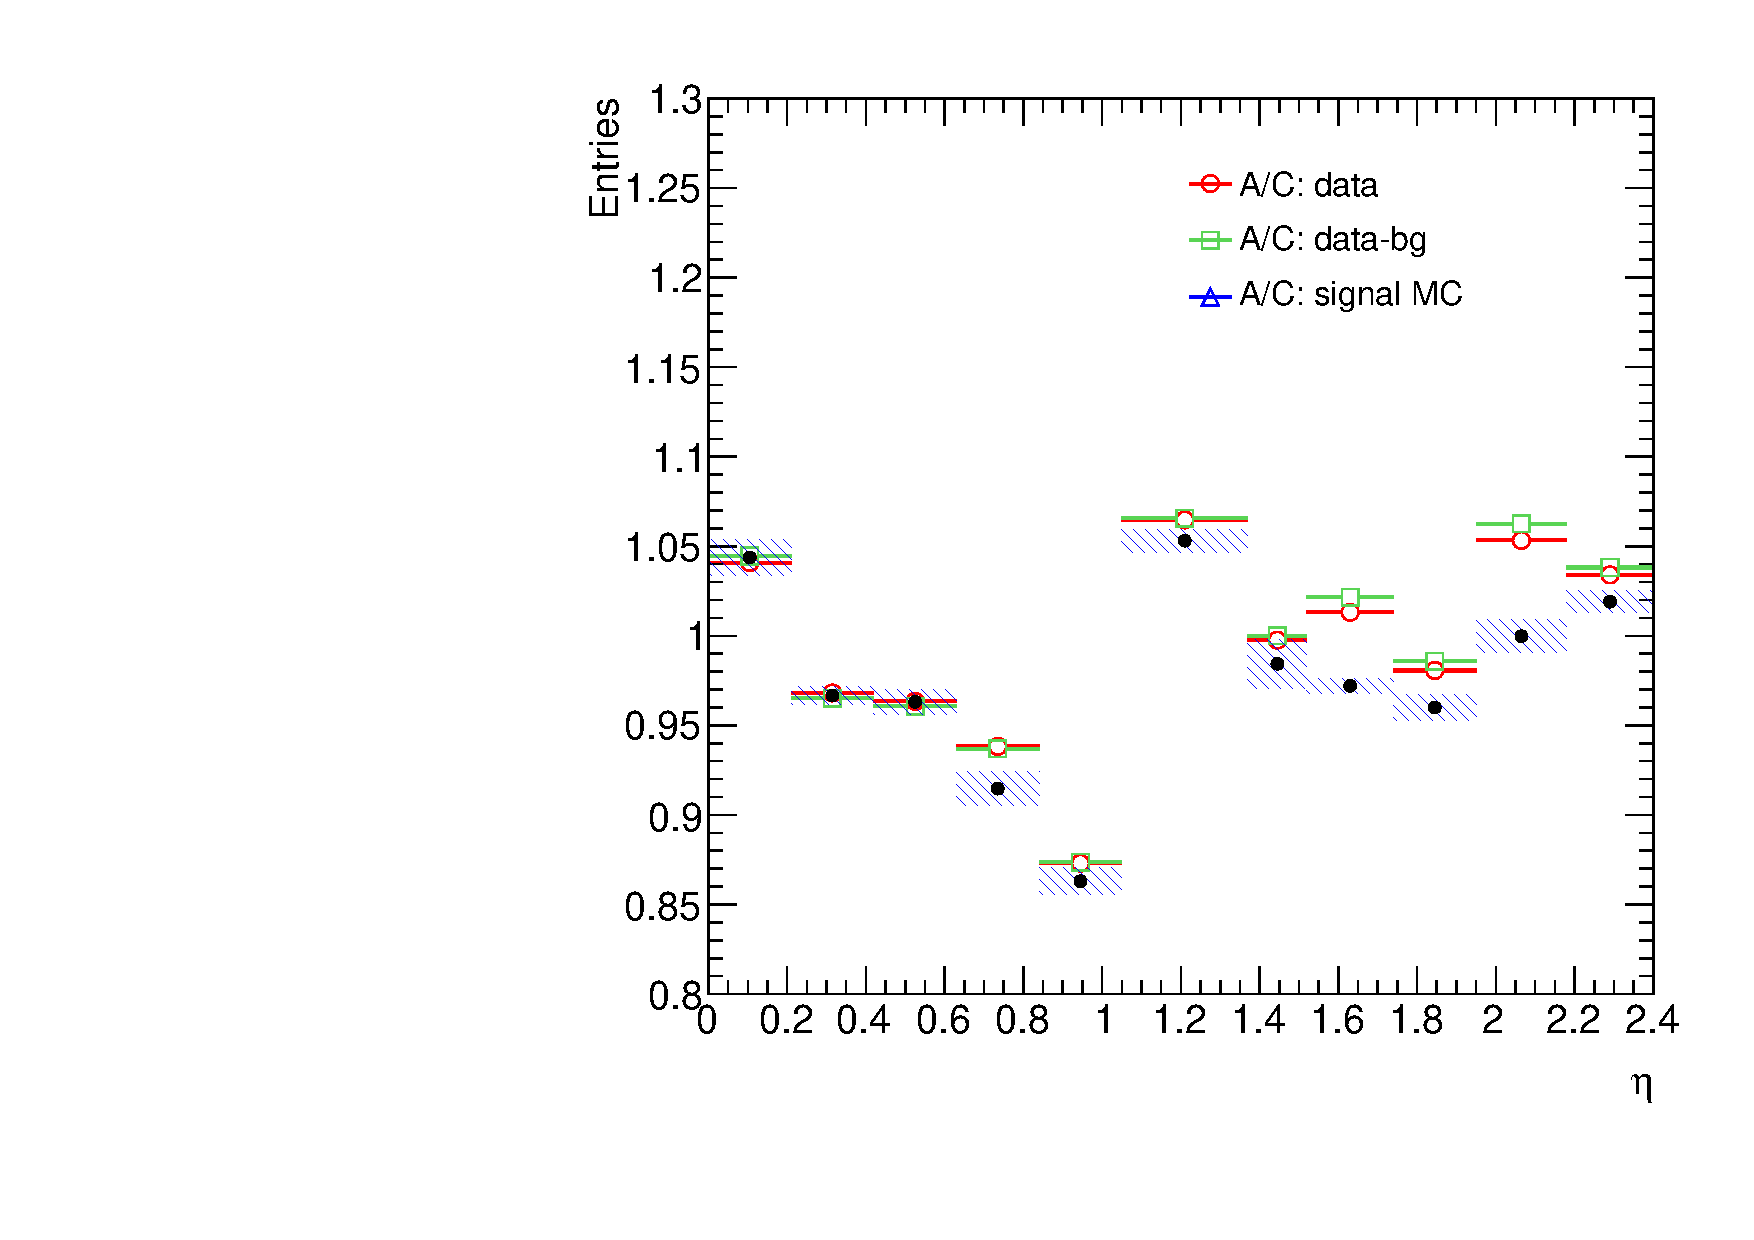
\includegraphics[width=1.0\textwidth]{dates/20130306/figures/both/W_NOM_Q0_stack_d3_eta_lpt_met_y_2__1_z_0__1_POS}
\column{.5\textwidth}
\centering
\small{ W (nominal), $\mu^{-}$}
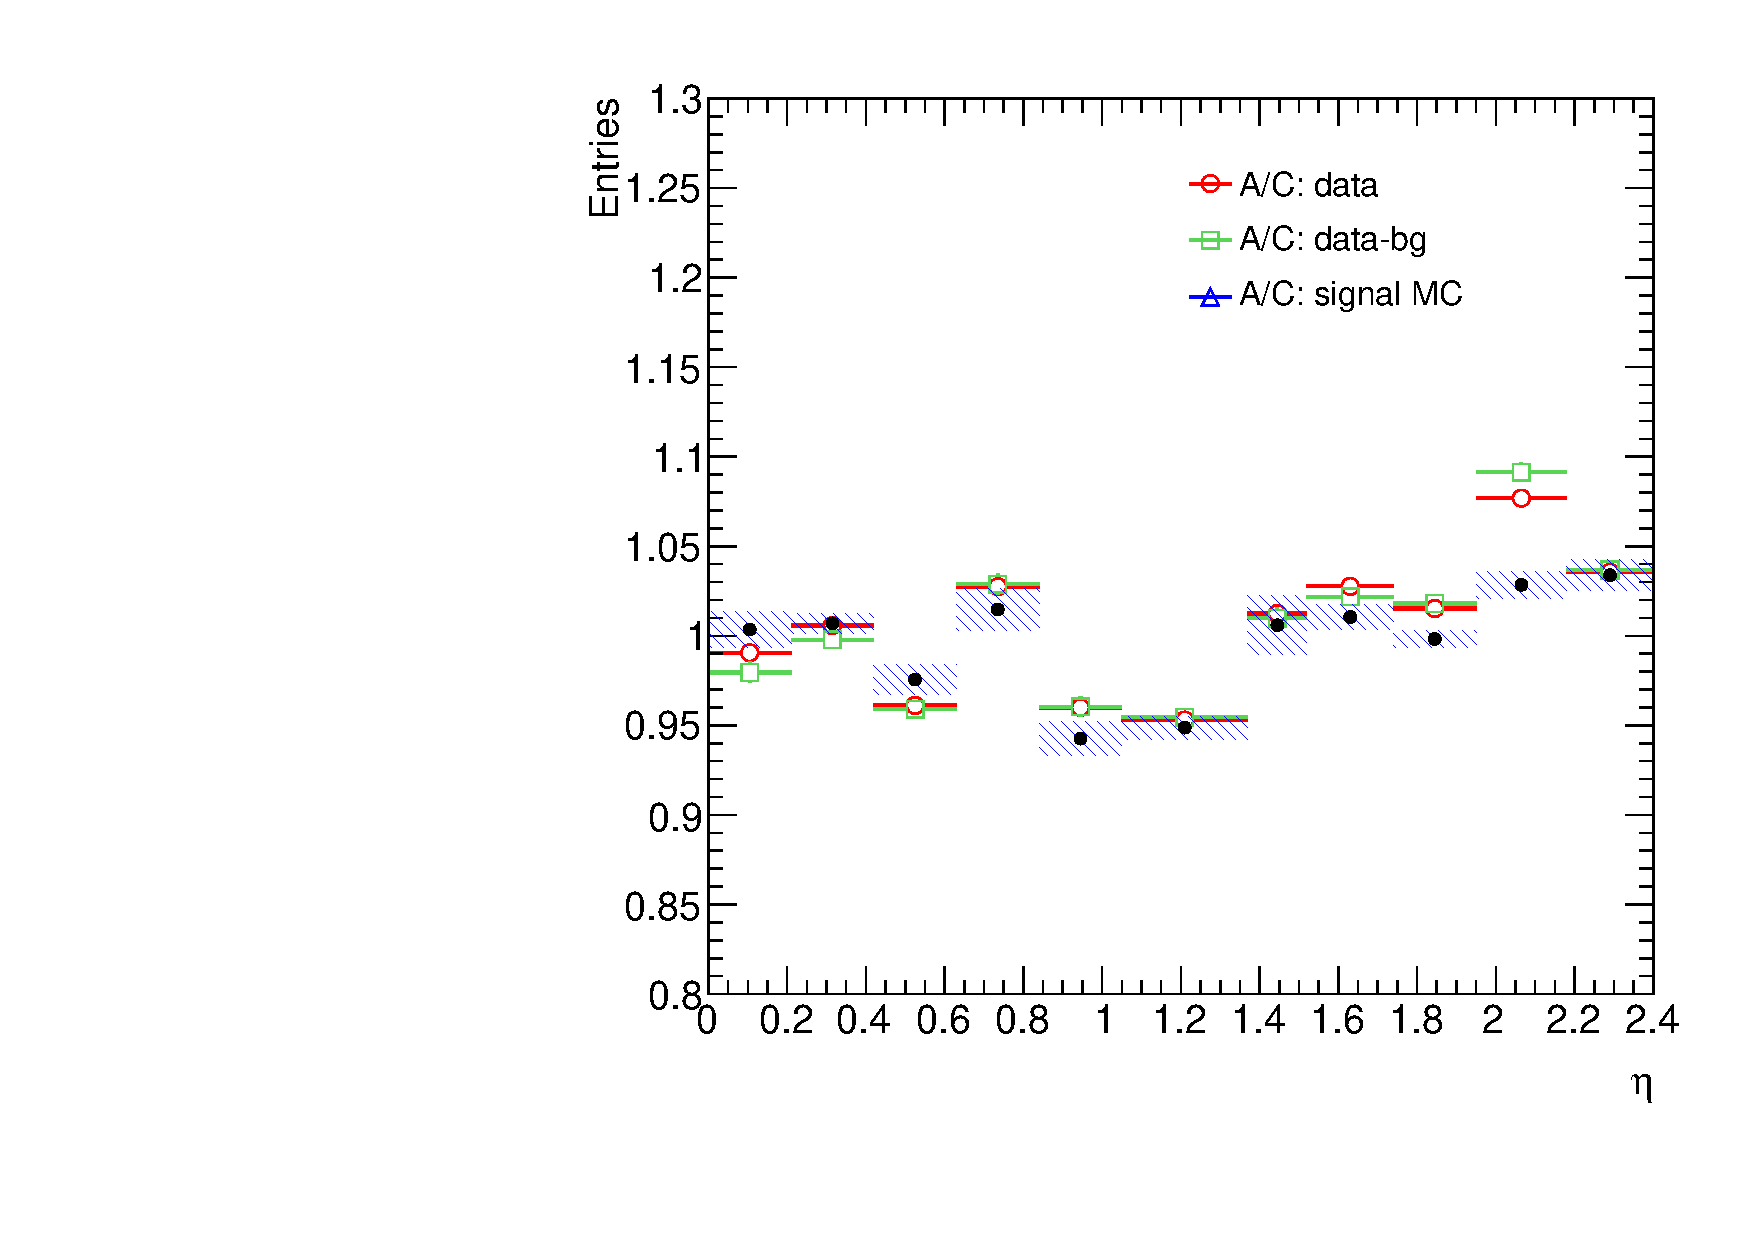
\includegraphics[width=1.0\textwidth]{dates/20130306/figures/both/W_NOM_Q0_stack_d3_eta_lpt_met_y_2__1_z_0__1_NEG}
\cole
}

\slide{ $\mu^{+}$: bin 10 ($1.95<\eta<2.18$) } {
\colb[T]
\column{.5\textwidth}
C-side $\mu^{+}$ (top: W; bottom: Z)
\centering
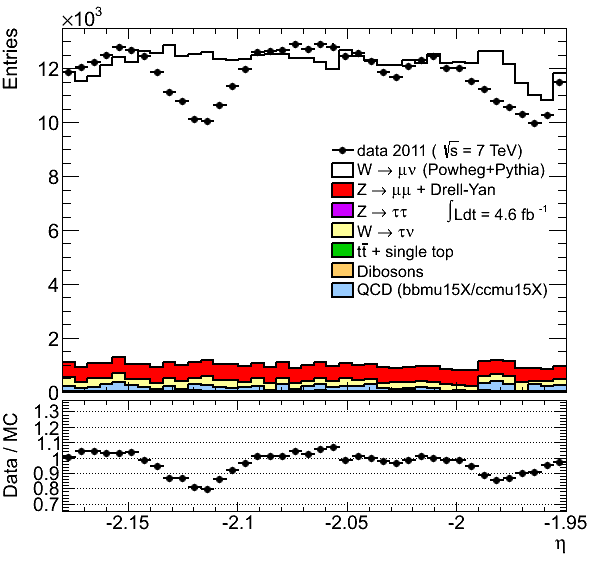
\includegraphics[width=0.66\textwidth]{dates/20130306/figures/both/W_10_C_stack_l_eta_POS} \\
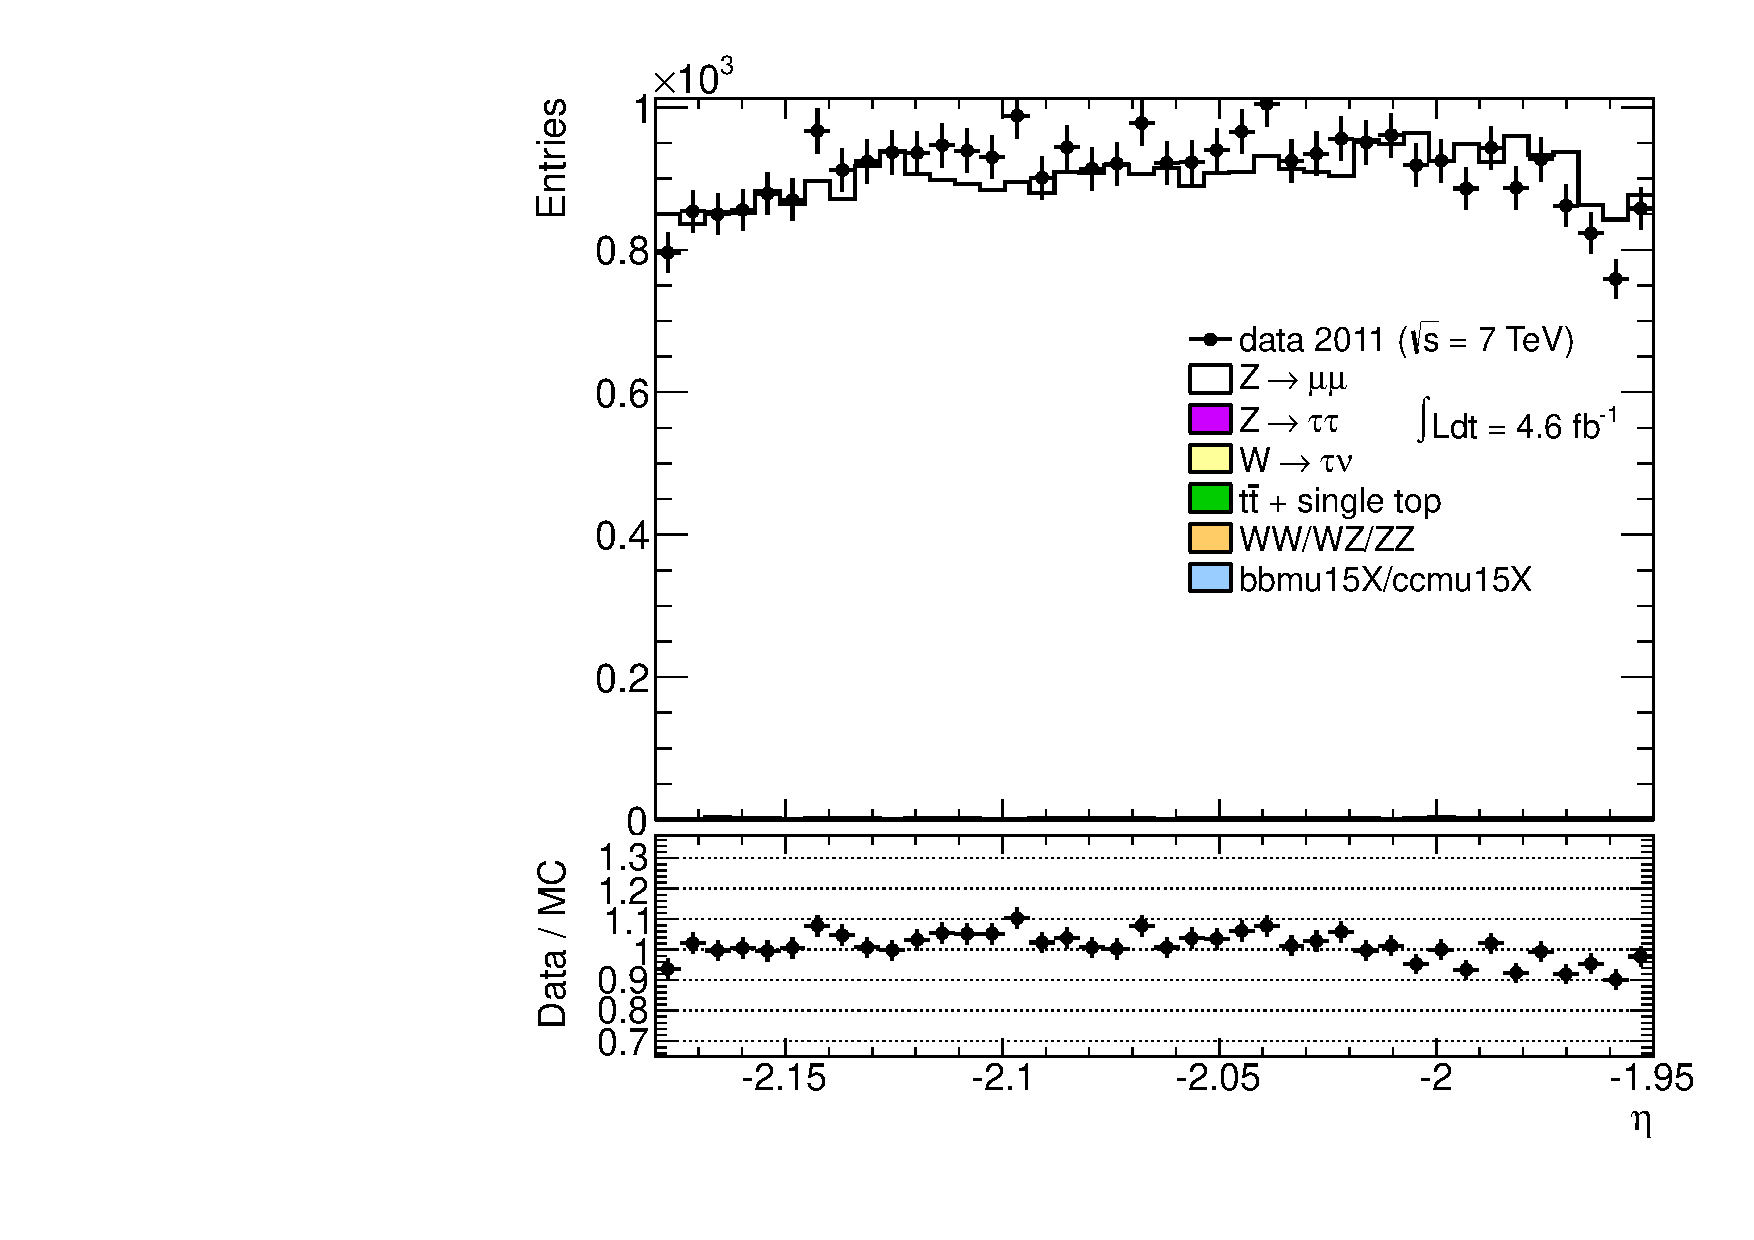
\includegraphics[width=0.66\textwidth]{dates/20130306/figures/both/Z_10_C_stack_lP_eta_ALL.pdf}
\column{.5\textwidth}
A-side $\mu^{+}$ (top: W; bottom: Z)
\centering
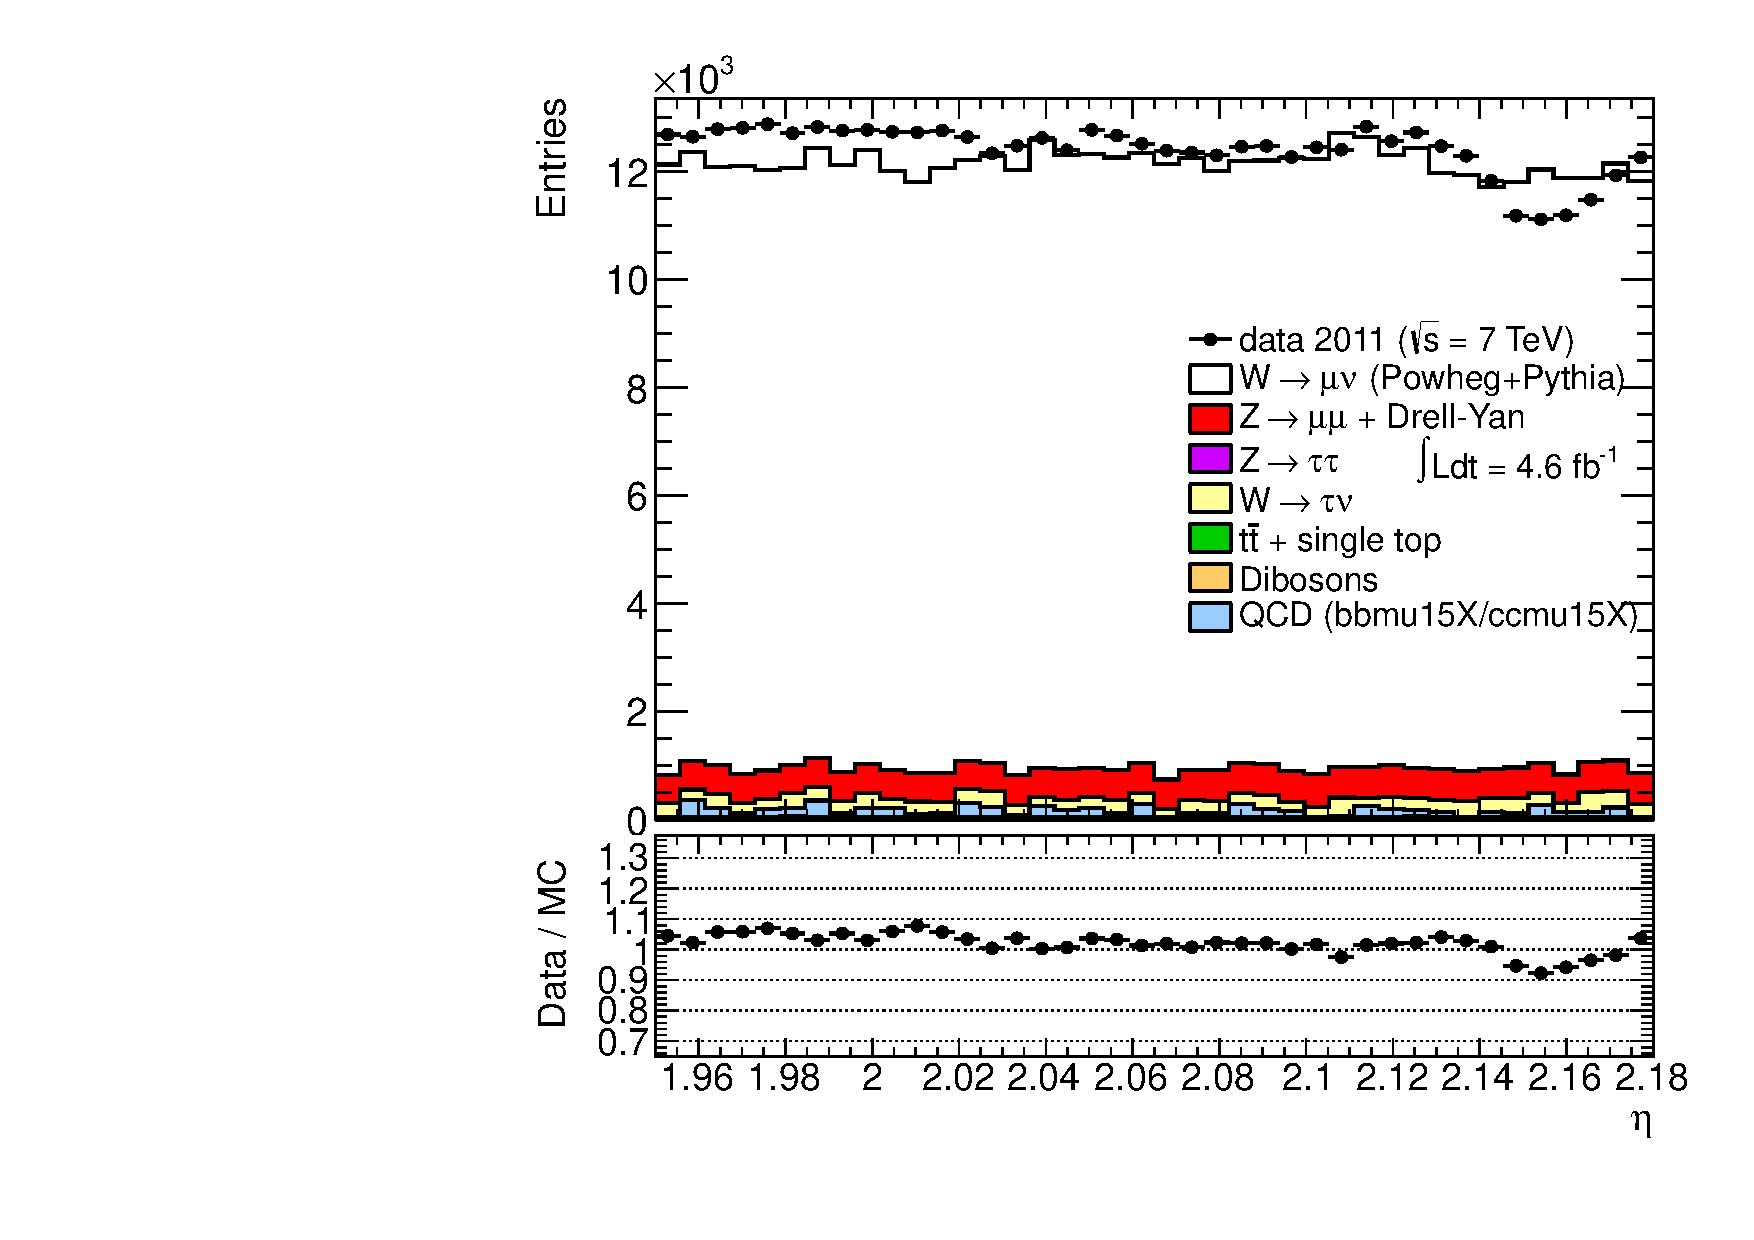
\includegraphics[width=0.66\textwidth]{dates/20130306/figures/both/W_10_A_stack_l_eta_POS} \\
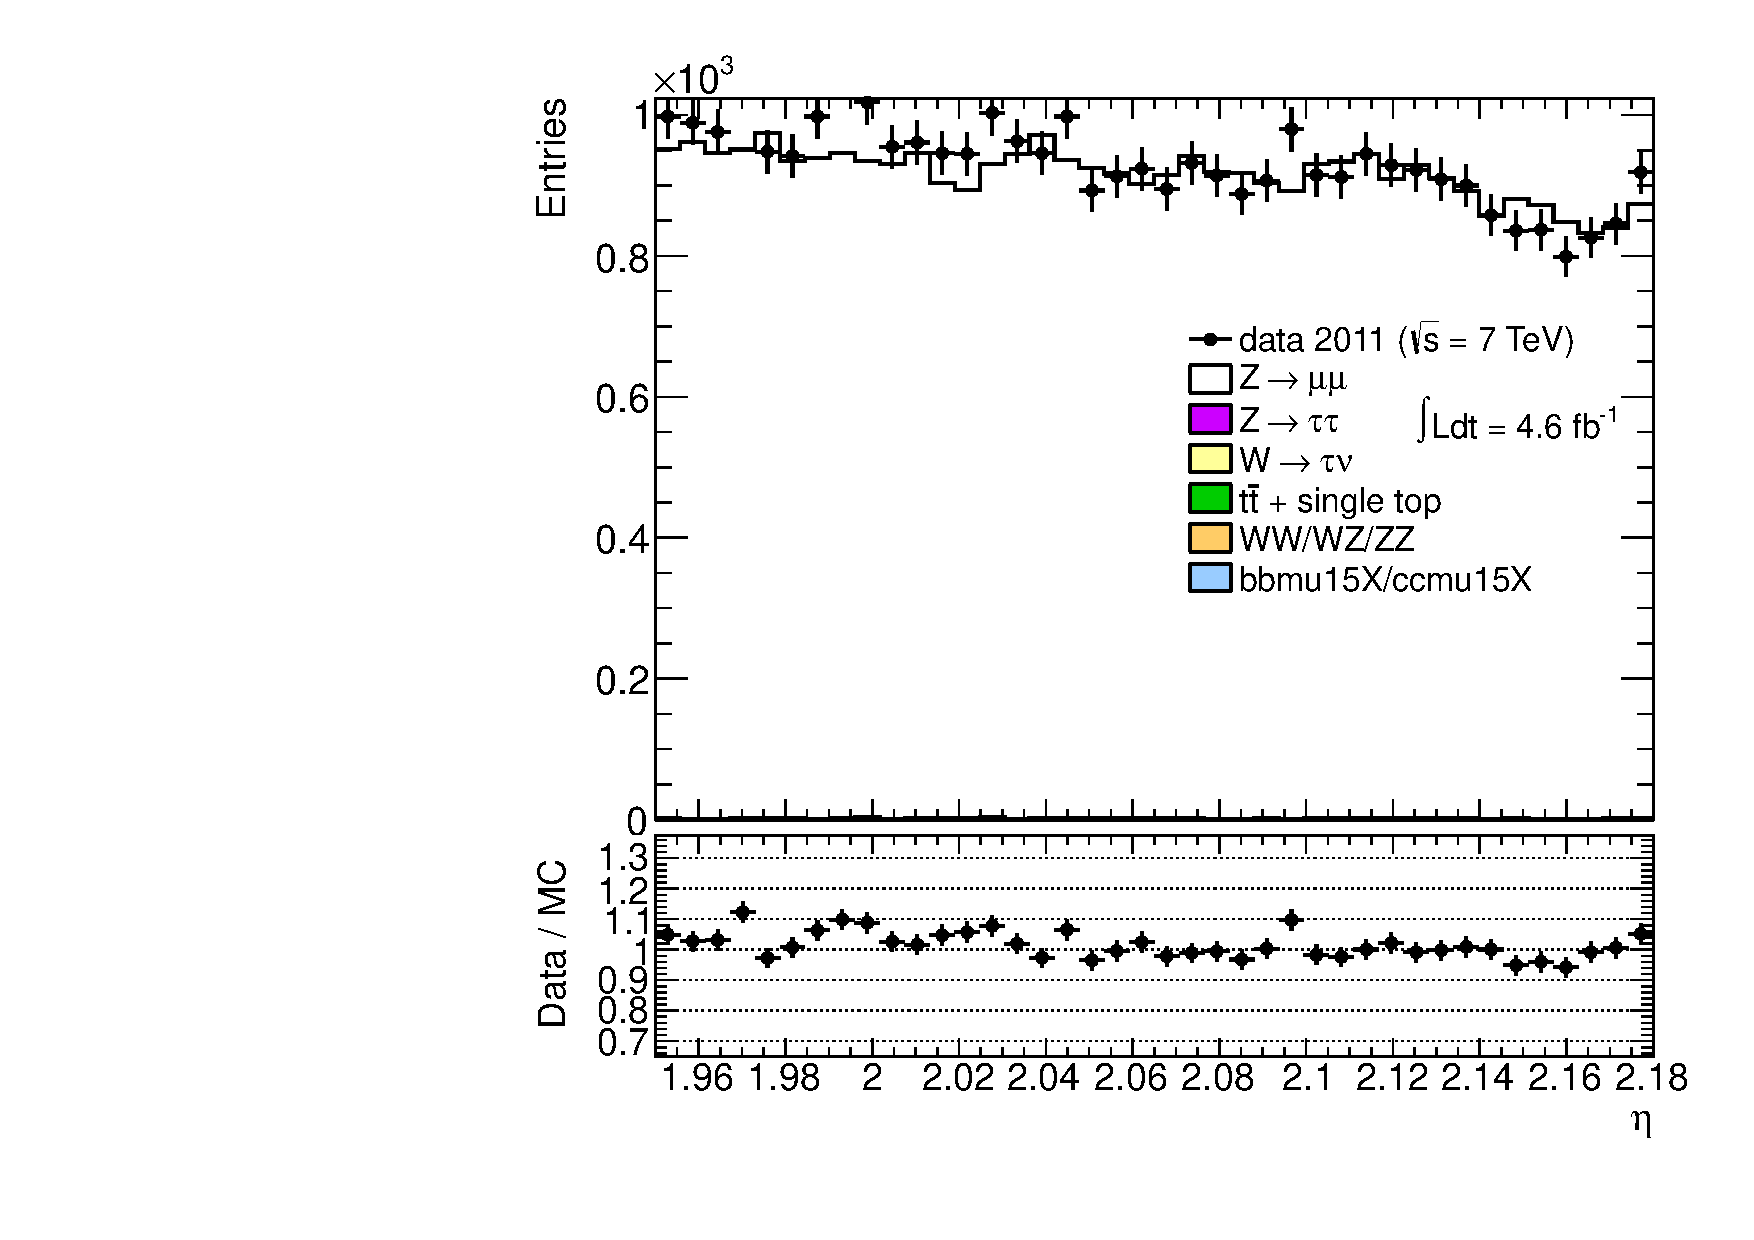
\includegraphics[width=0.66\textwidth]{dates/20130306/figures/both/Z_10_A_stack_lP_eta_ALL.pdf} 
\cole
}

\slide{ $\mu^{-}$: bin 10 ($1.95<\eta<2.18$) } {
\colb[T]
\column{.5\textwidth}
C-side $\mu^{-}$ (top: W; bottom: Z)
\centering
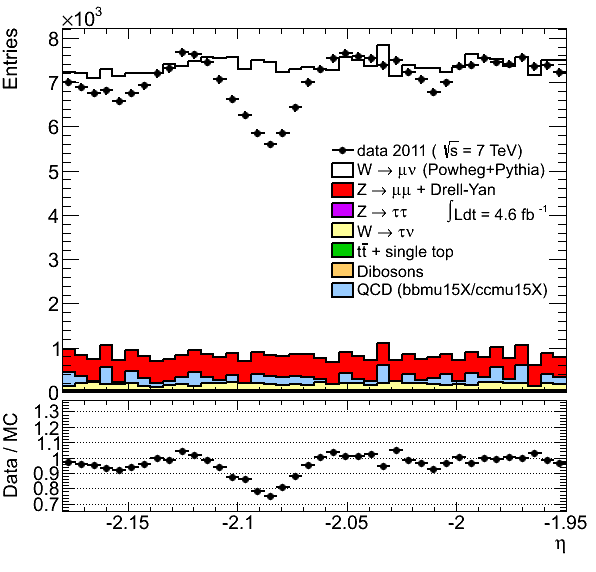
\includegraphics[width=0.66\textwidth]{dates/20130306/figures/both/W_10_C_stack_l_eta_NEG} \\
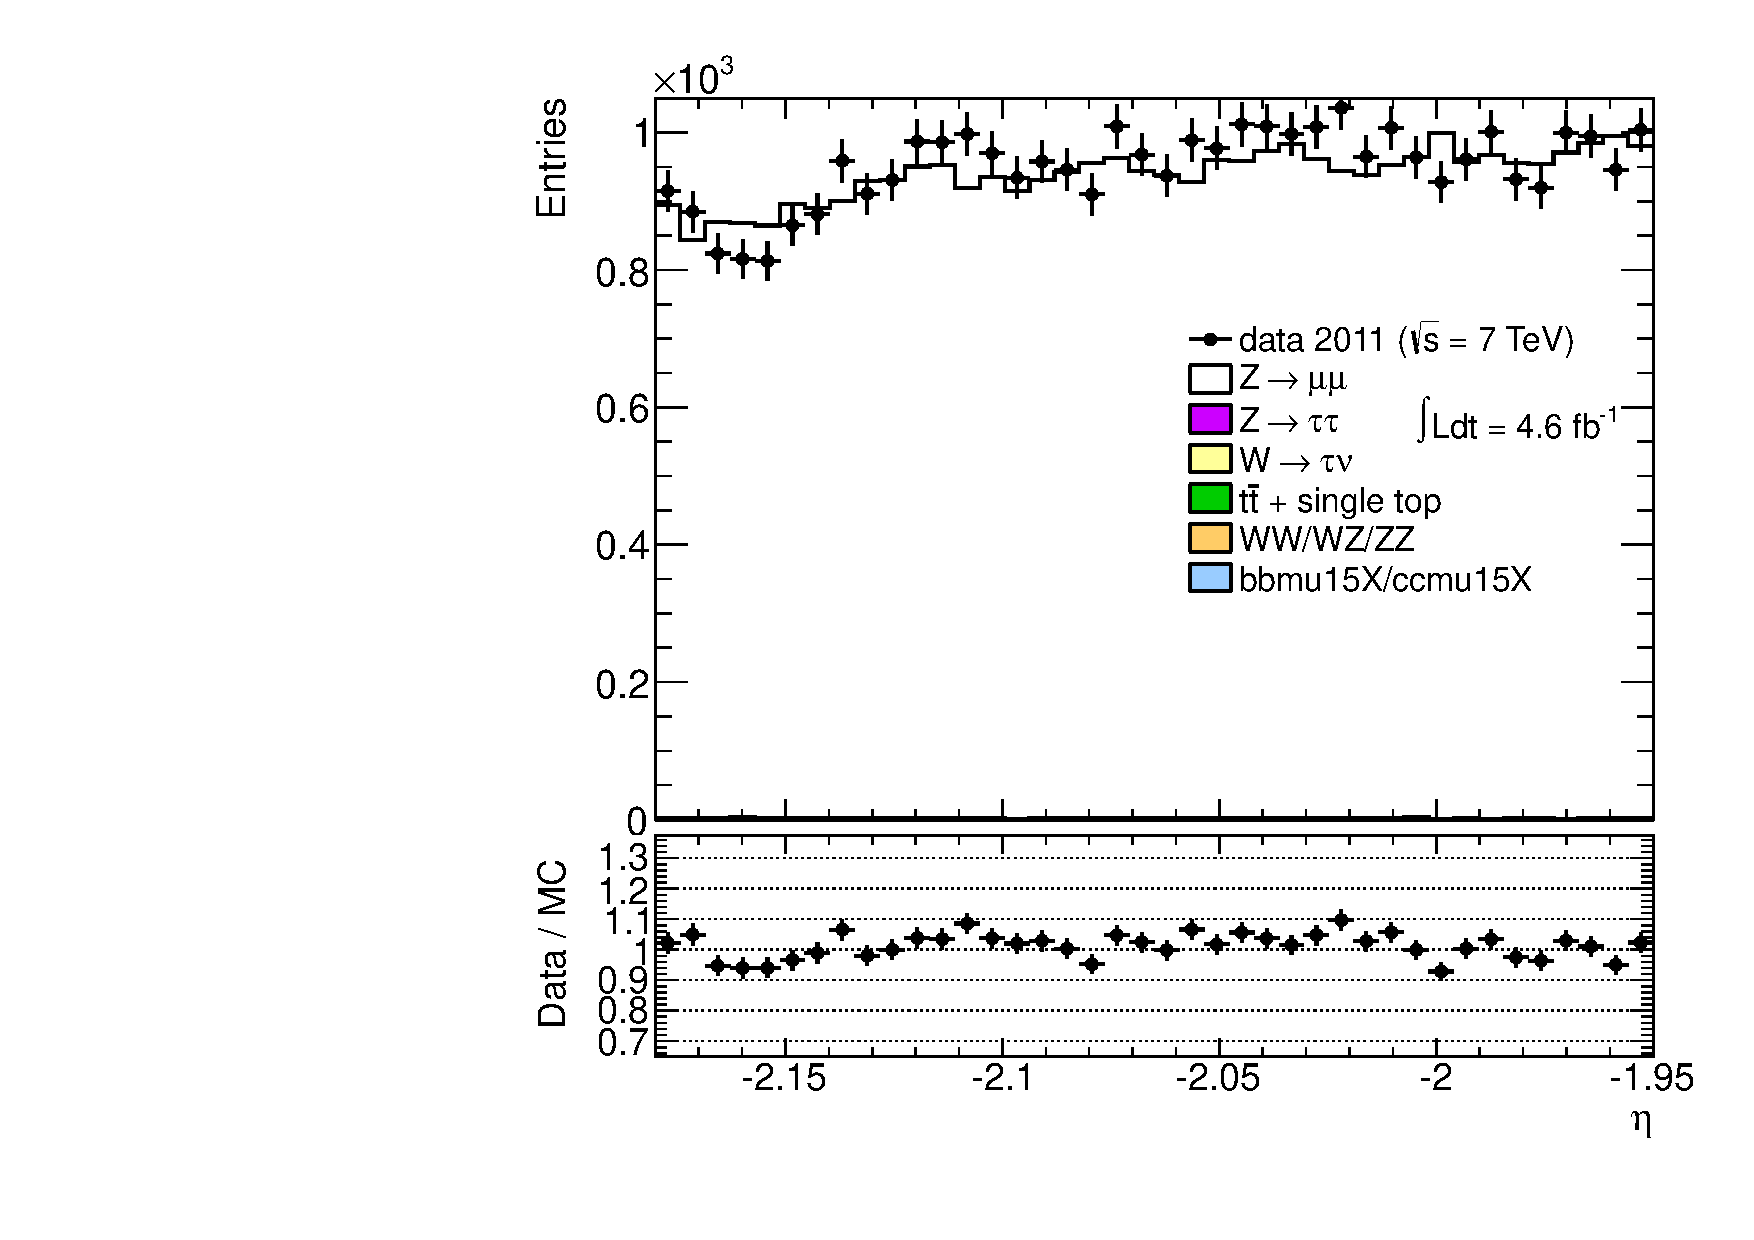
\includegraphics[width=0.66\textwidth]{dates/20130306/figures/both/Z_10_C_stack_lN_eta_ALL.pdf}
\column{.5\textwidth}
A-side $\mu^{-}$ (top: W; bottom: Z)
\centering
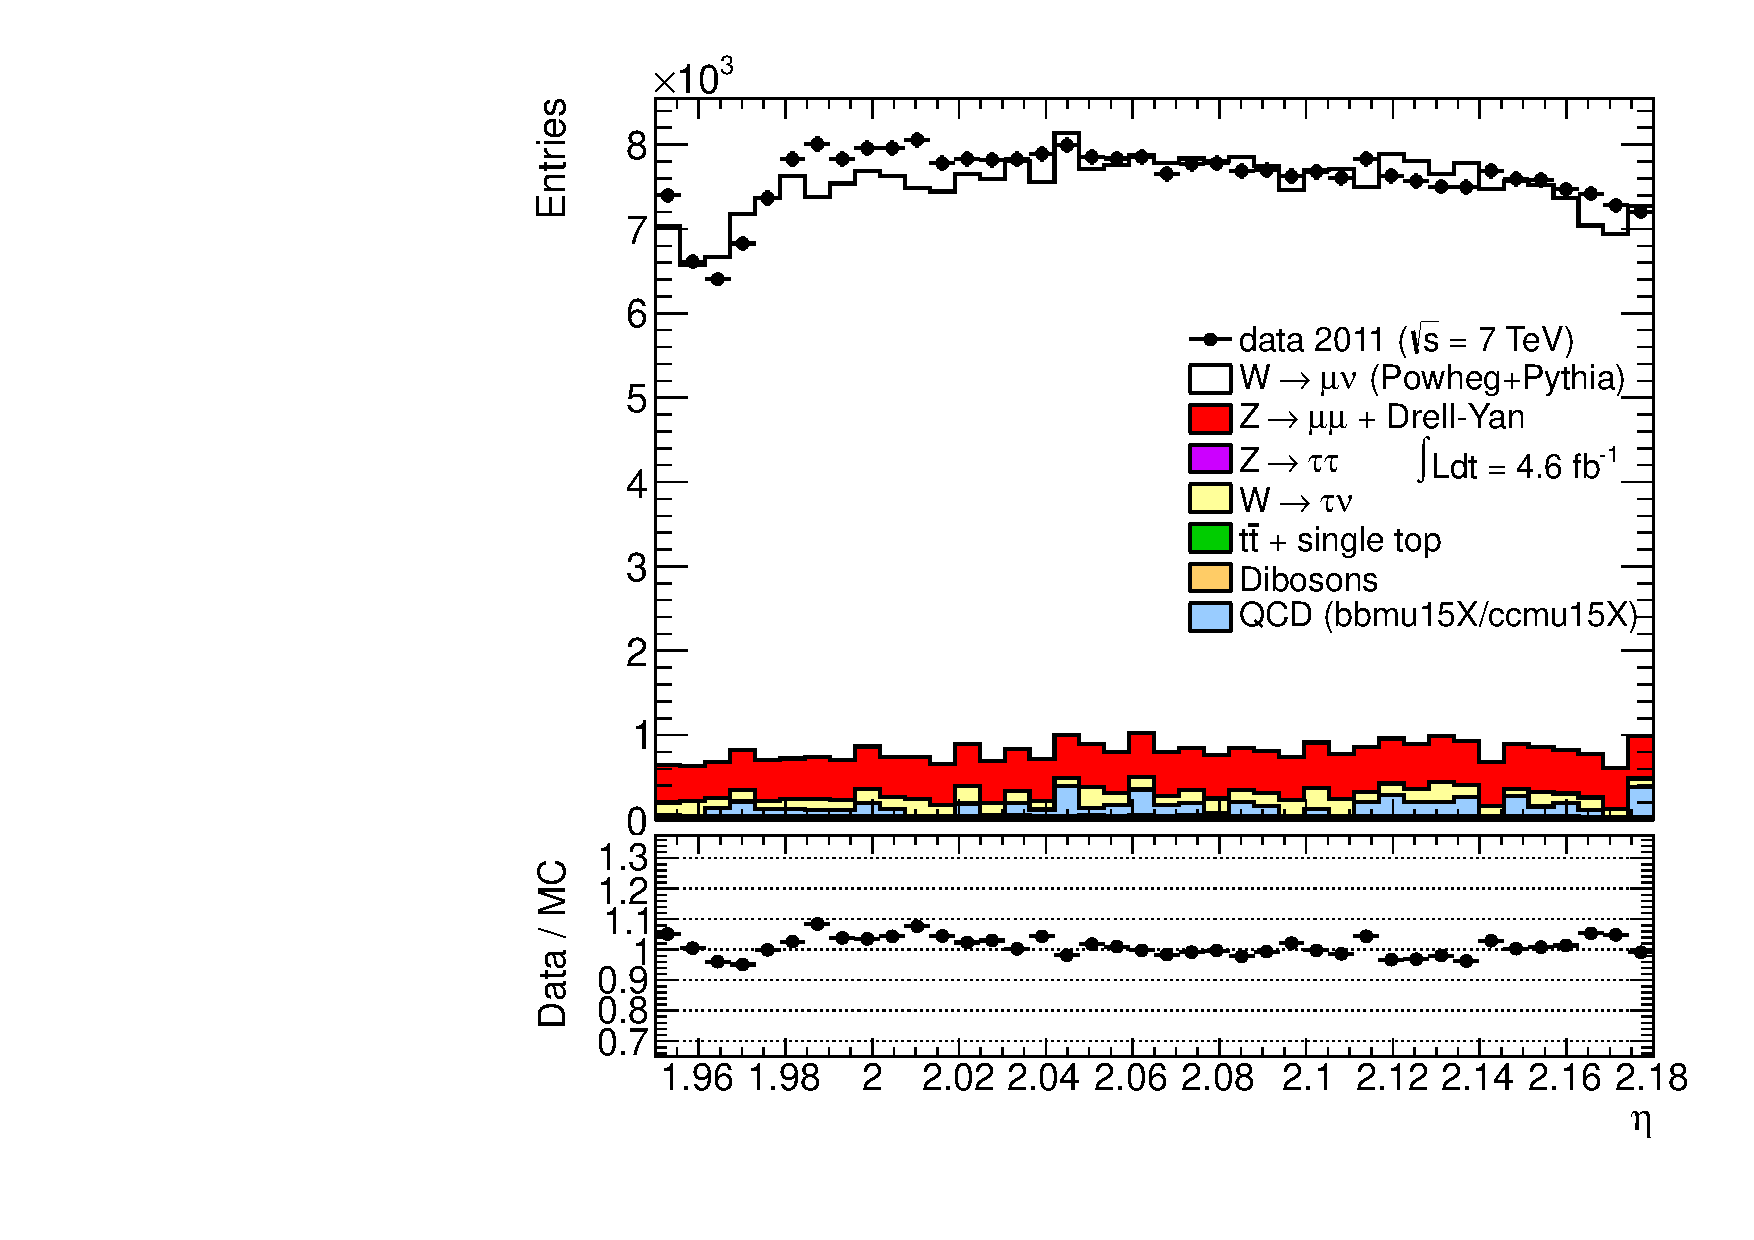
\includegraphics[width=0.66\textwidth]{dates/20130306/figures/both/W_10_A_stack_l_eta_NEG} \\
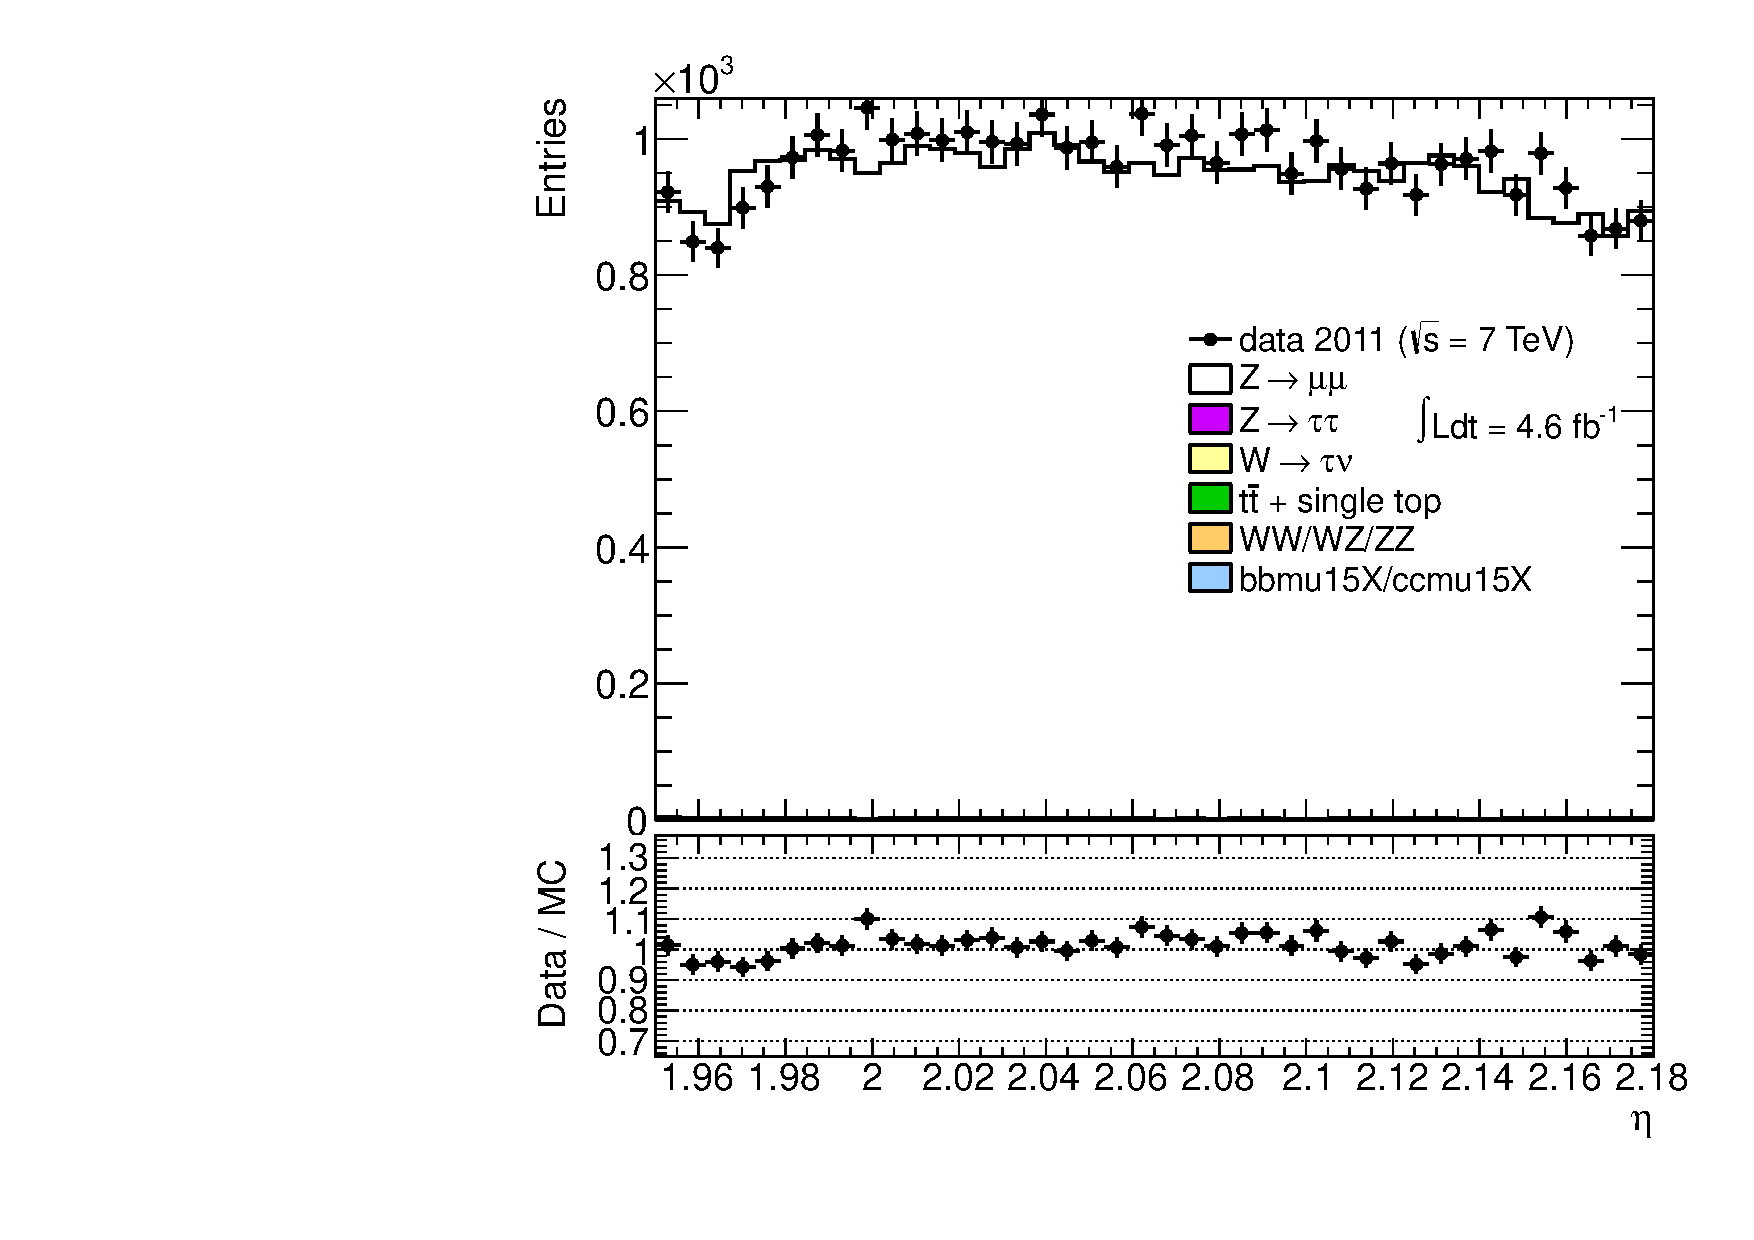
\includegraphics[width=0.66\textwidth]{dates/20130306/figures/both/Z_10_A_stack_lN_eta_ALL.pdf} 
\cole
}

\slide{ $\mu^{-}$: MET } {
Well, W has MET. \\
Let's remove MET and WMT cuts from W. \\
(notice enhanced QCD in the W plots)
}
\slide{ $\mu^{-}$: MET } {
\colb[T]
\column{.5\textwidth}
C-side $\mu^{-}$ (top: W; bottom: Z)
\centering
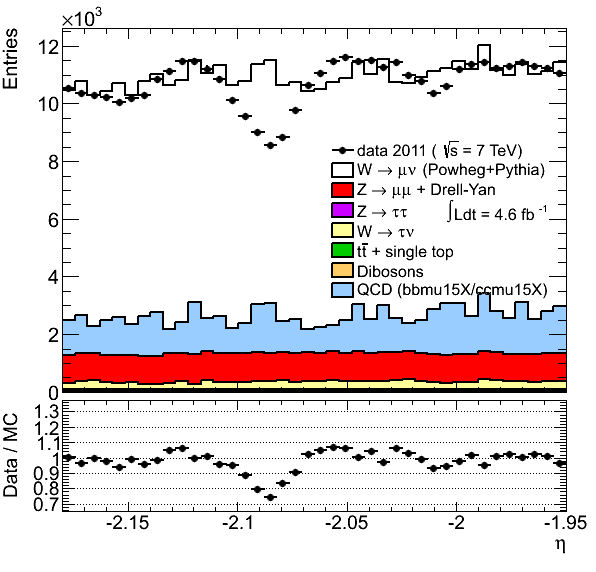
\includegraphics[width=0.66\textwidth]{dates/20130306/figures/both/Wnometmt_10_C_stack_l_eta_NEG} \\
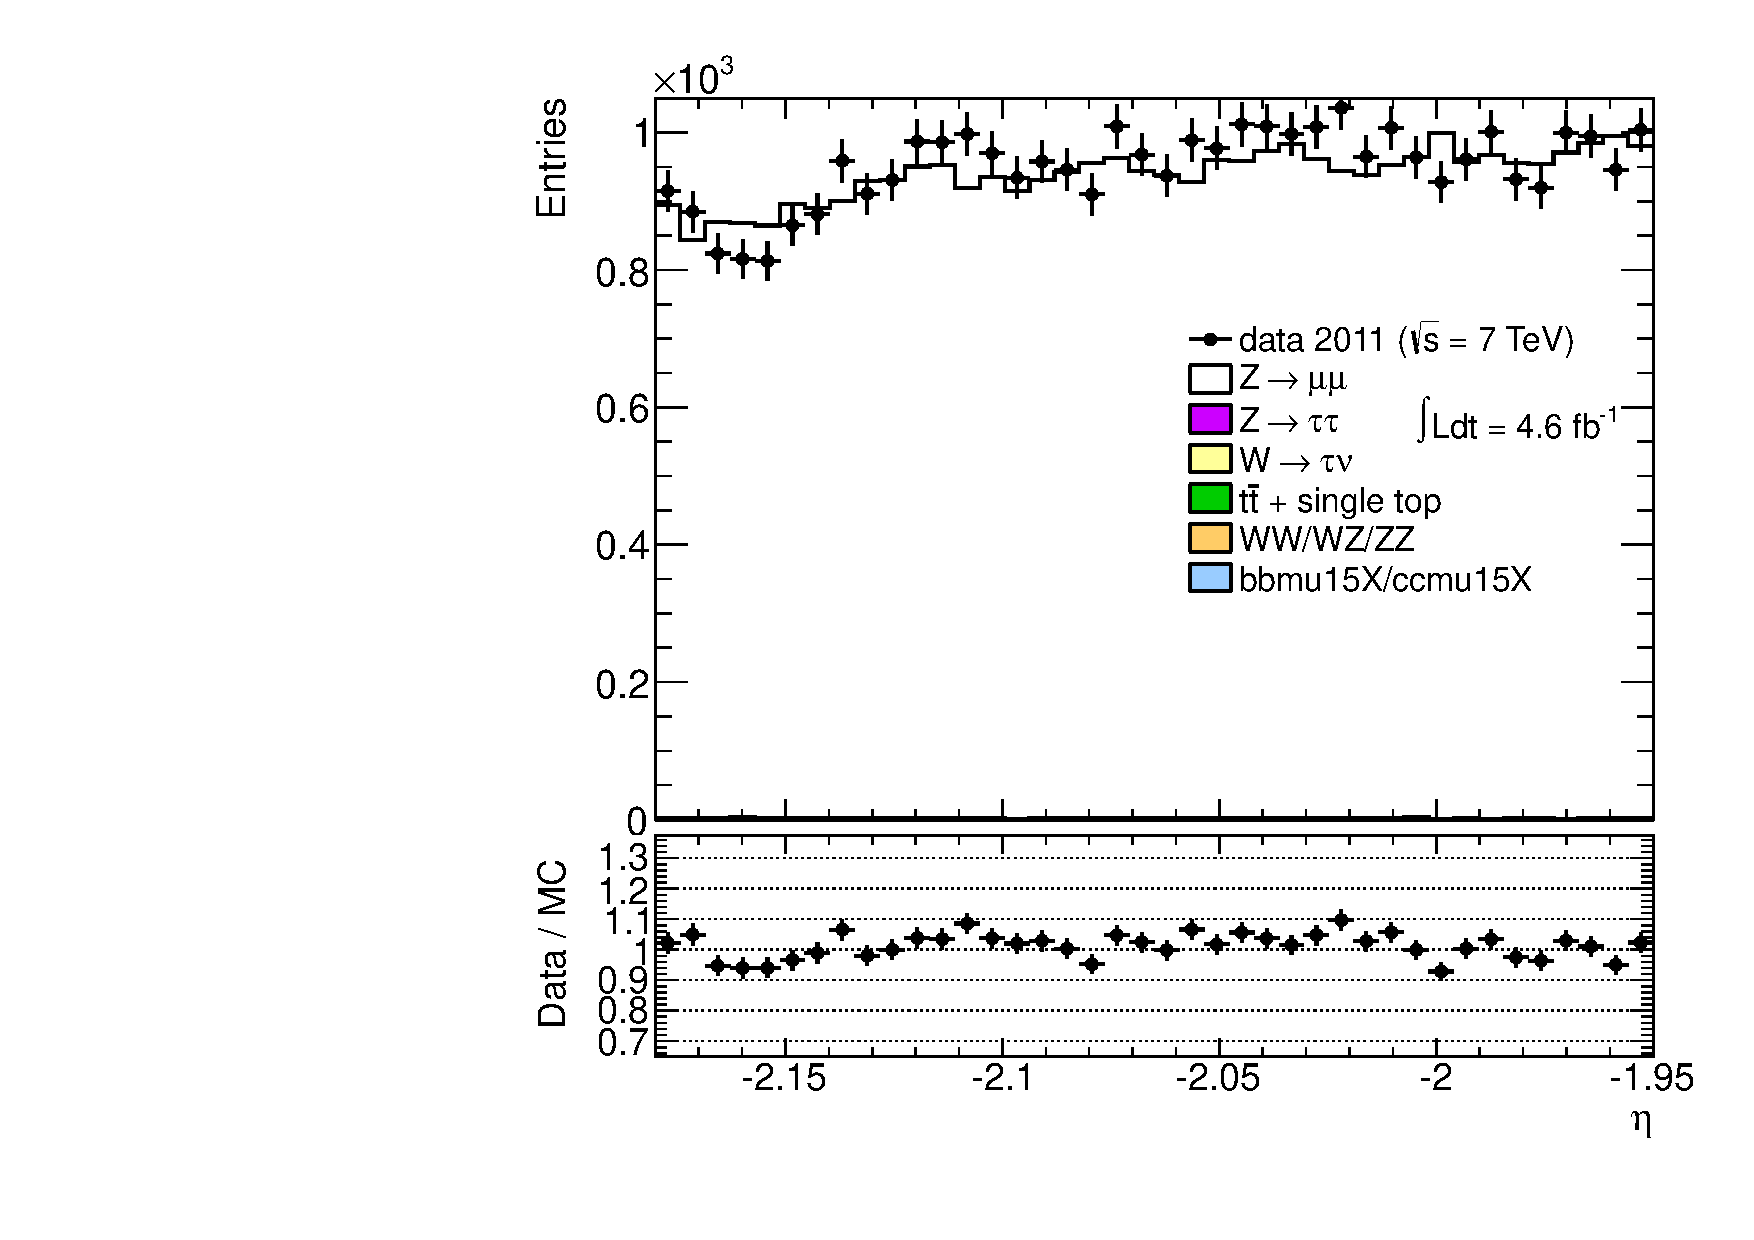
\includegraphics[width=0.66\textwidth]{dates/20130306/figures/both/Z_10_C_stack_lN_eta_ALL.pdf}
\column{.5\textwidth}
A-side $\mu^{-}$ (top: W; bottom: Z)
\centering
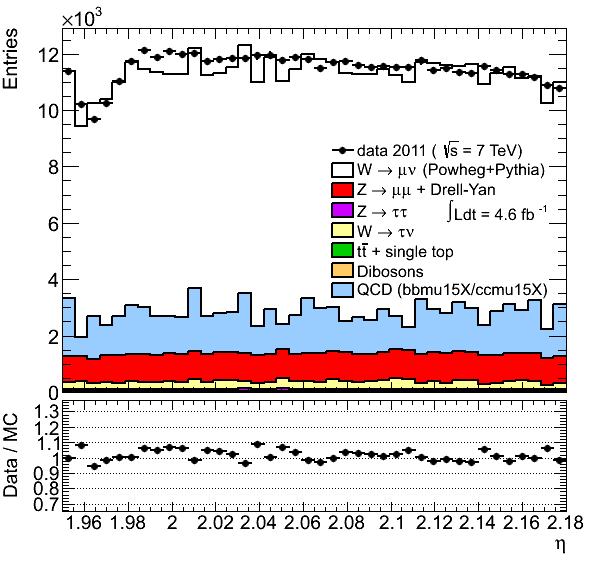
\includegraphics[width=0.66\textwidth]{dates/20130306/figures/both/Wnometmt_10_A_stack_l_eta_NEG} \\
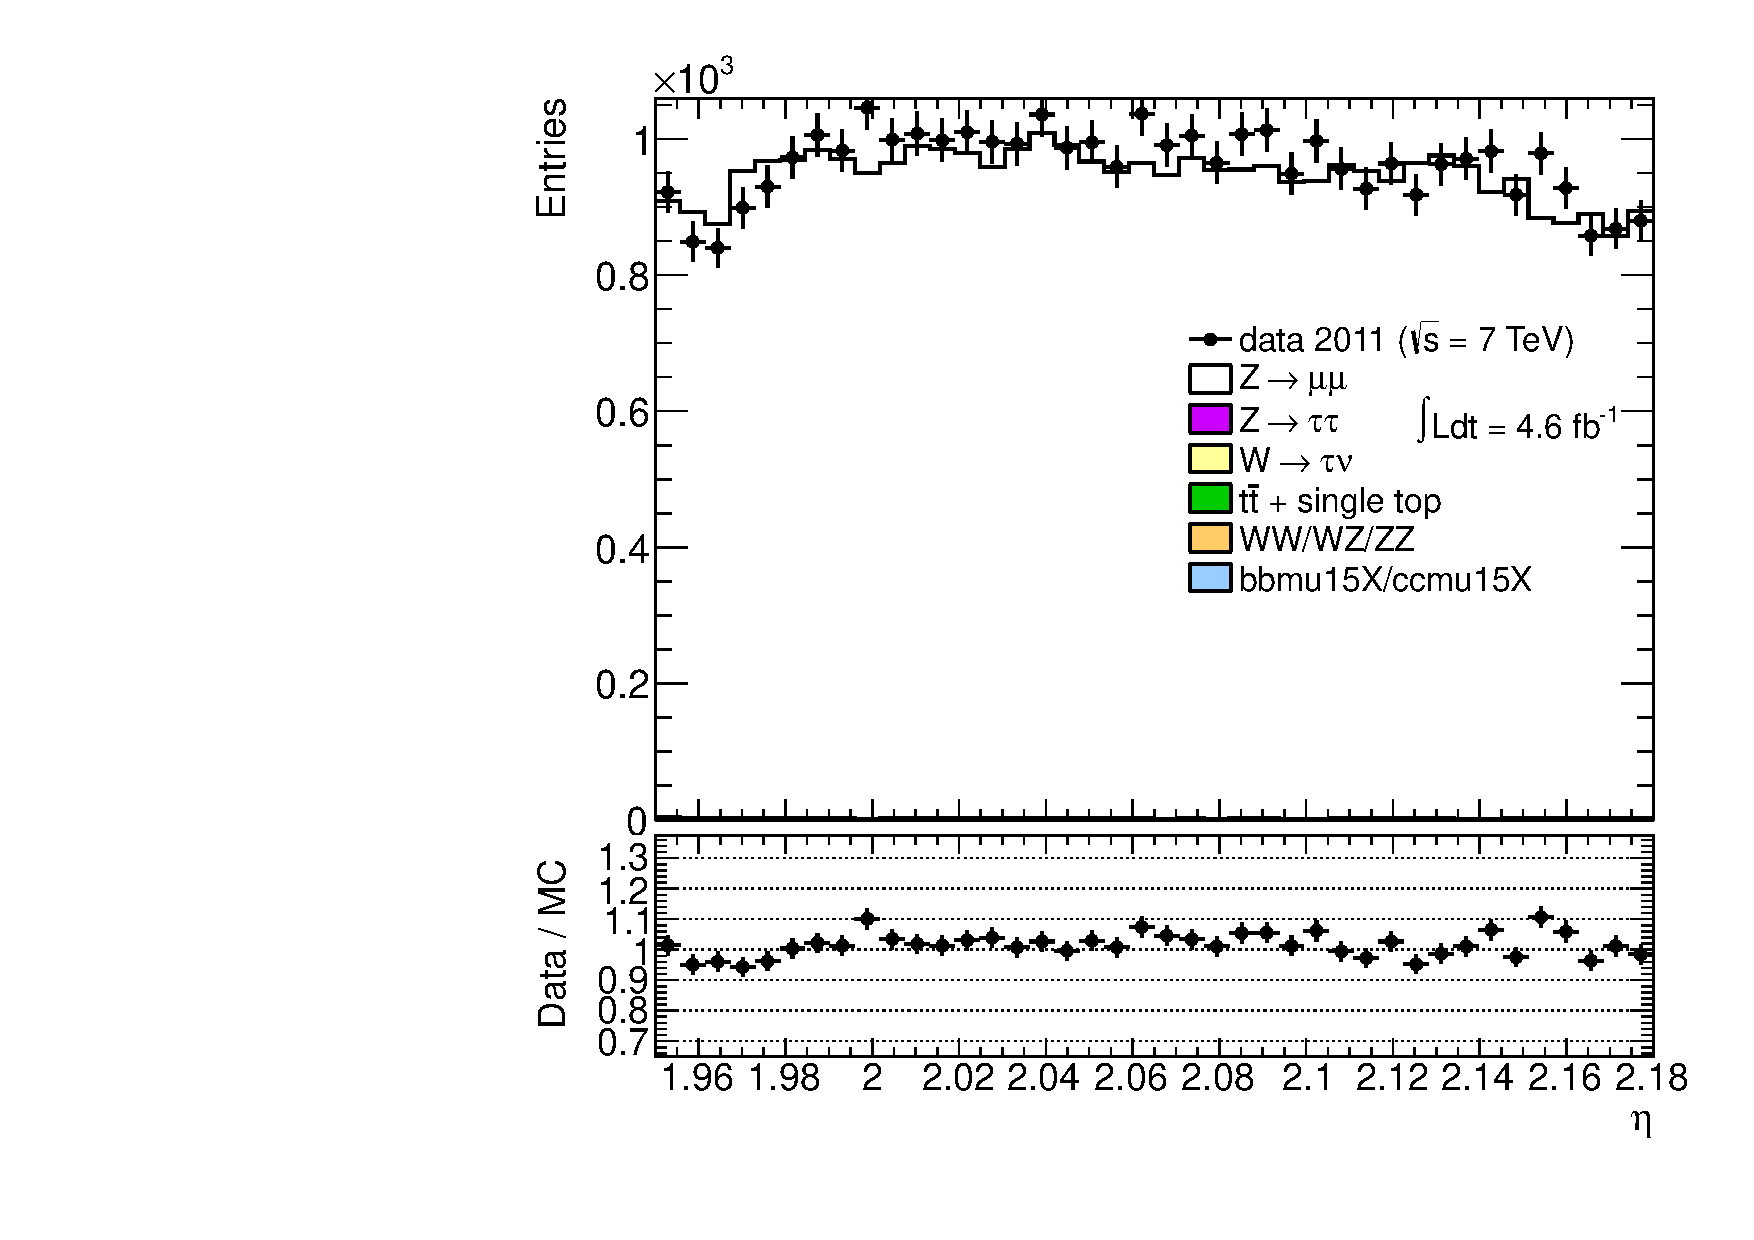
\includegraphics[width=0.66\textwidth]{dates/20130306/figures/both/Z_10_A_stack_lN_eta_ALL.pdf} 
\cole
}

\slide{ $\mu^{-}$: min. pT } {
Z boson is a little heavier and may give off more energetic muons. \\
What if the lower-pT muons in the W channel produce the dip? \\
Let's try to bump up pT cut to 35 GeV on both W and Z muons.
}
\slide{ $\mu^{-}$: min. pT } {
\colb[T]
\column{.5\textwidth}
C-side $\mu^{-}$ (top: W; bottom: Z)
\centering
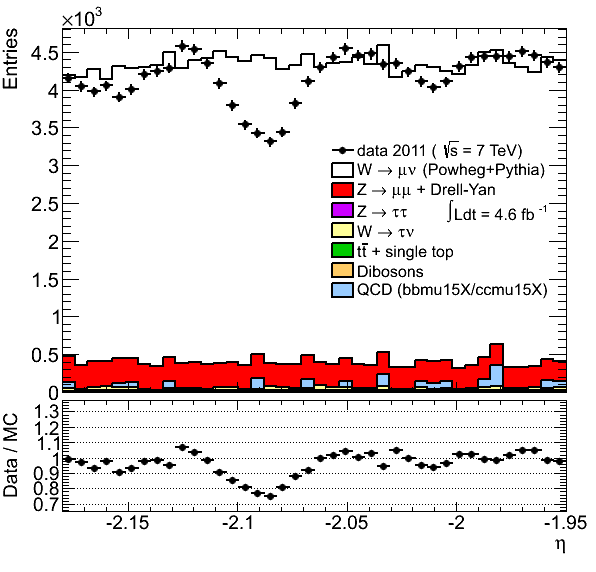
\includegraphics[width=0.66\textwidth]{dates/20130306/figures/both/Wpt35_10_C_stack_l_eta_NEG} \\
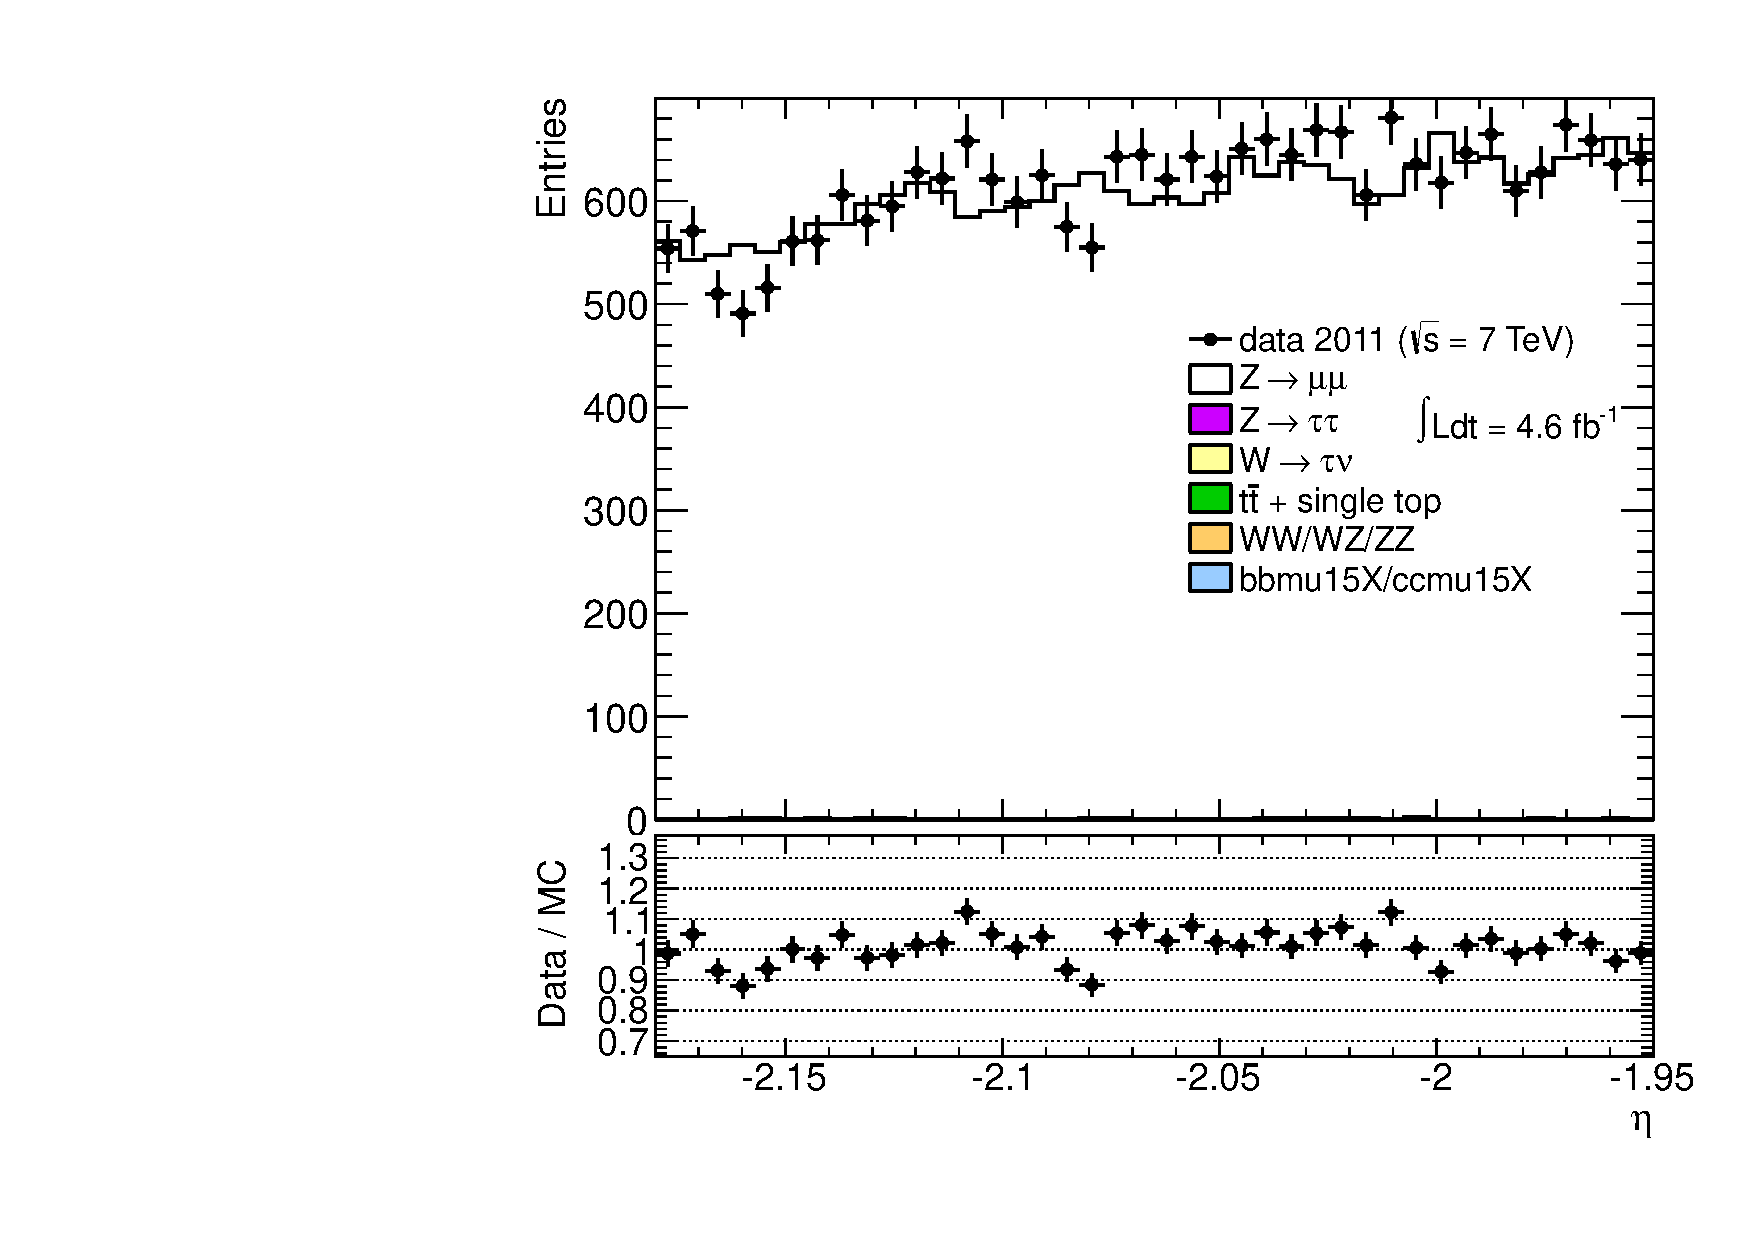
\includegraphics[width=0.66\textwidth]{dates/20130306/figures/both/Zpt35_10_C_stack_lN_eta_ALL.pdf}
\column{.5\textwidth}
A-side $\mu^{-}$ (top: W; bottom: Z)
\centering
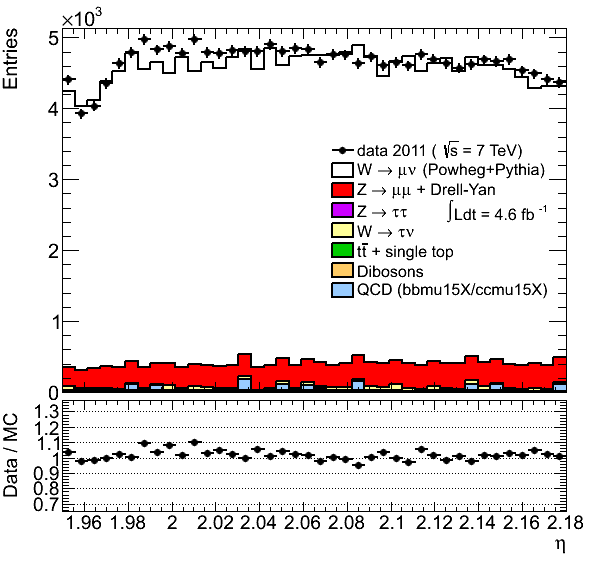
\includegraphics[width=0.66\textwidth]{dates/20130306/figures/both/Wpt35_10_A_stack_l_eta_NEG} \\
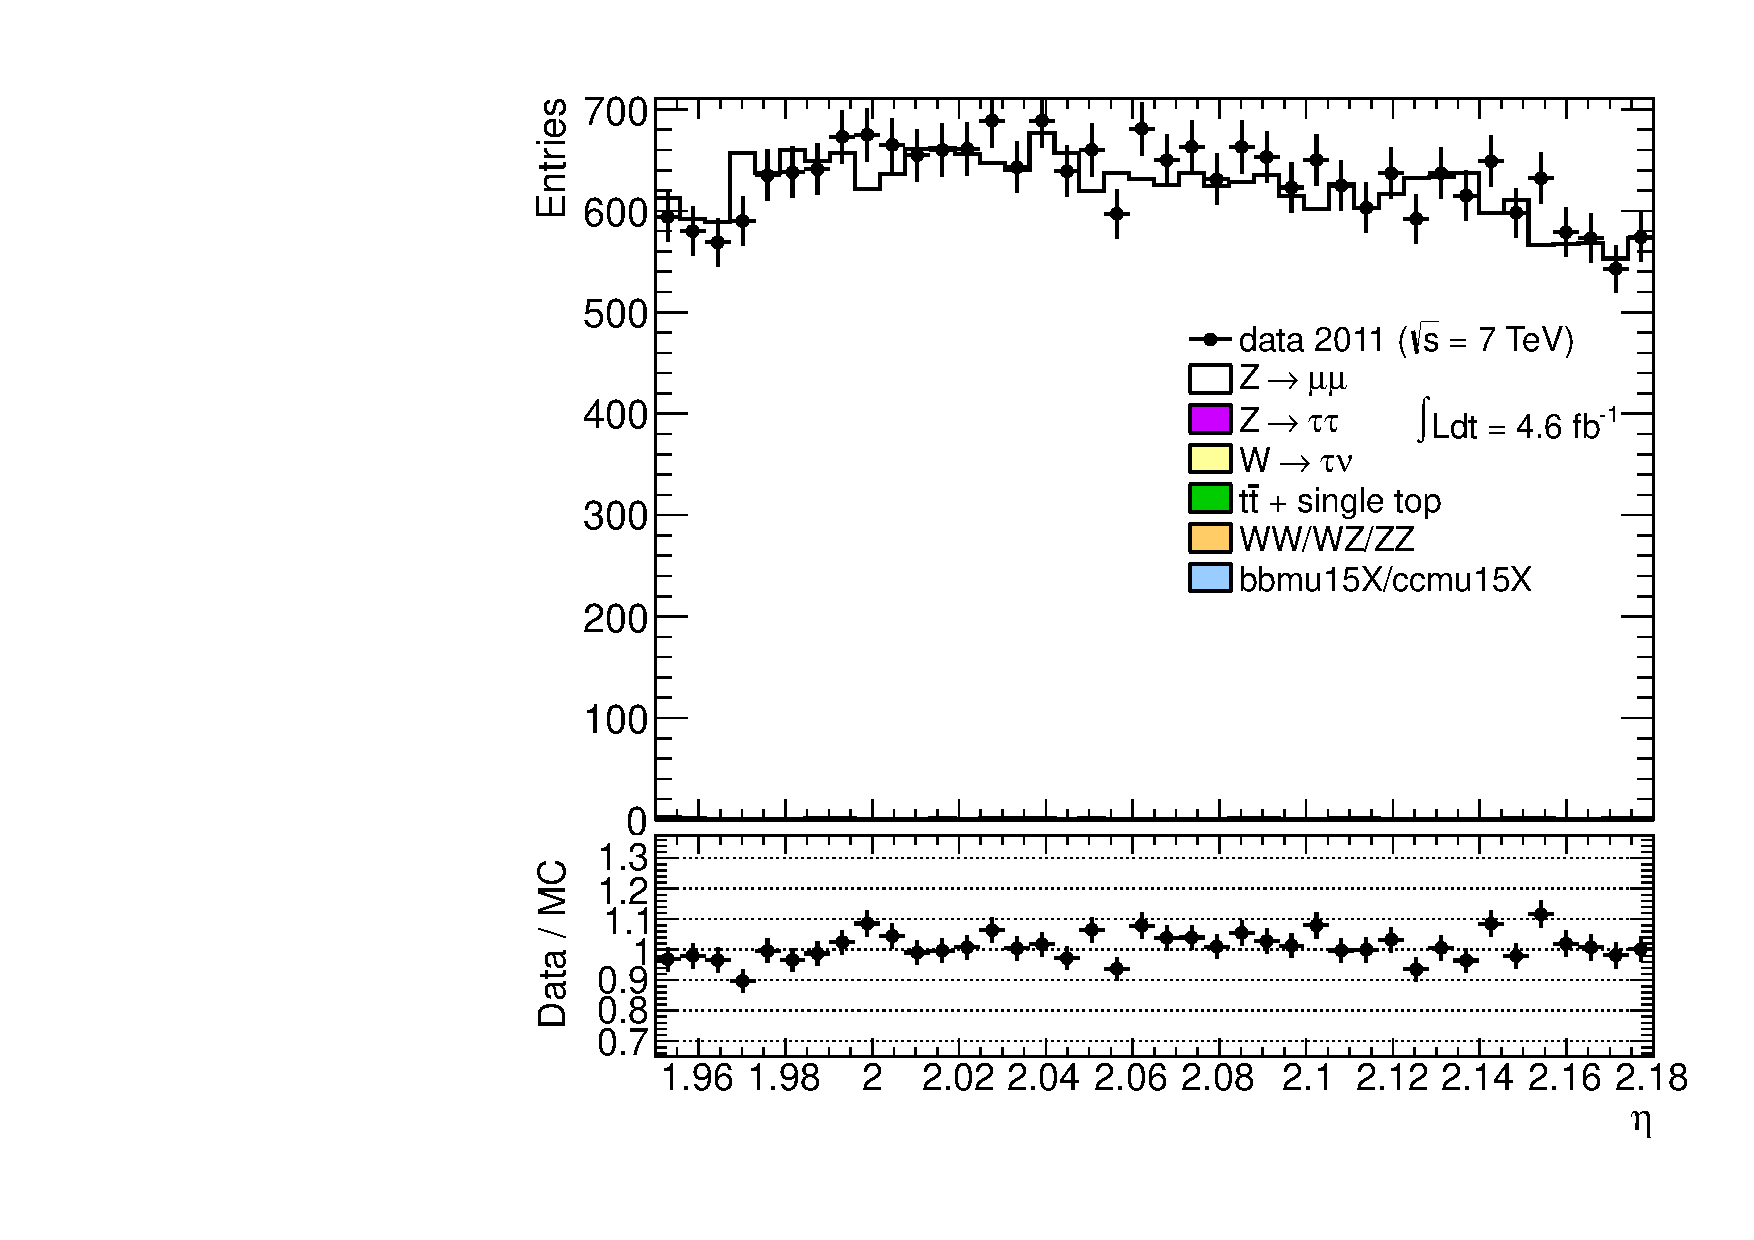
\includegraphics[width=0.66\textwidth]{dates/20130306/figures/both/Zpt35_10_A_stack_lN_eta_ALL.pdf} 
\cole
}

\slide{ $\mu^{-}$: max. pT } {
For completeness, let's try to put an upper cap on pT: \\
Limit pT range to 25-35 GeV for both W and Z muons
}
\slide{ $\mu^{-}$: max. pT } {
\colb[T]
\column{.5\textwidth}
C-side $\mu^{-}$ (top: W; bottom: Z)
\centering
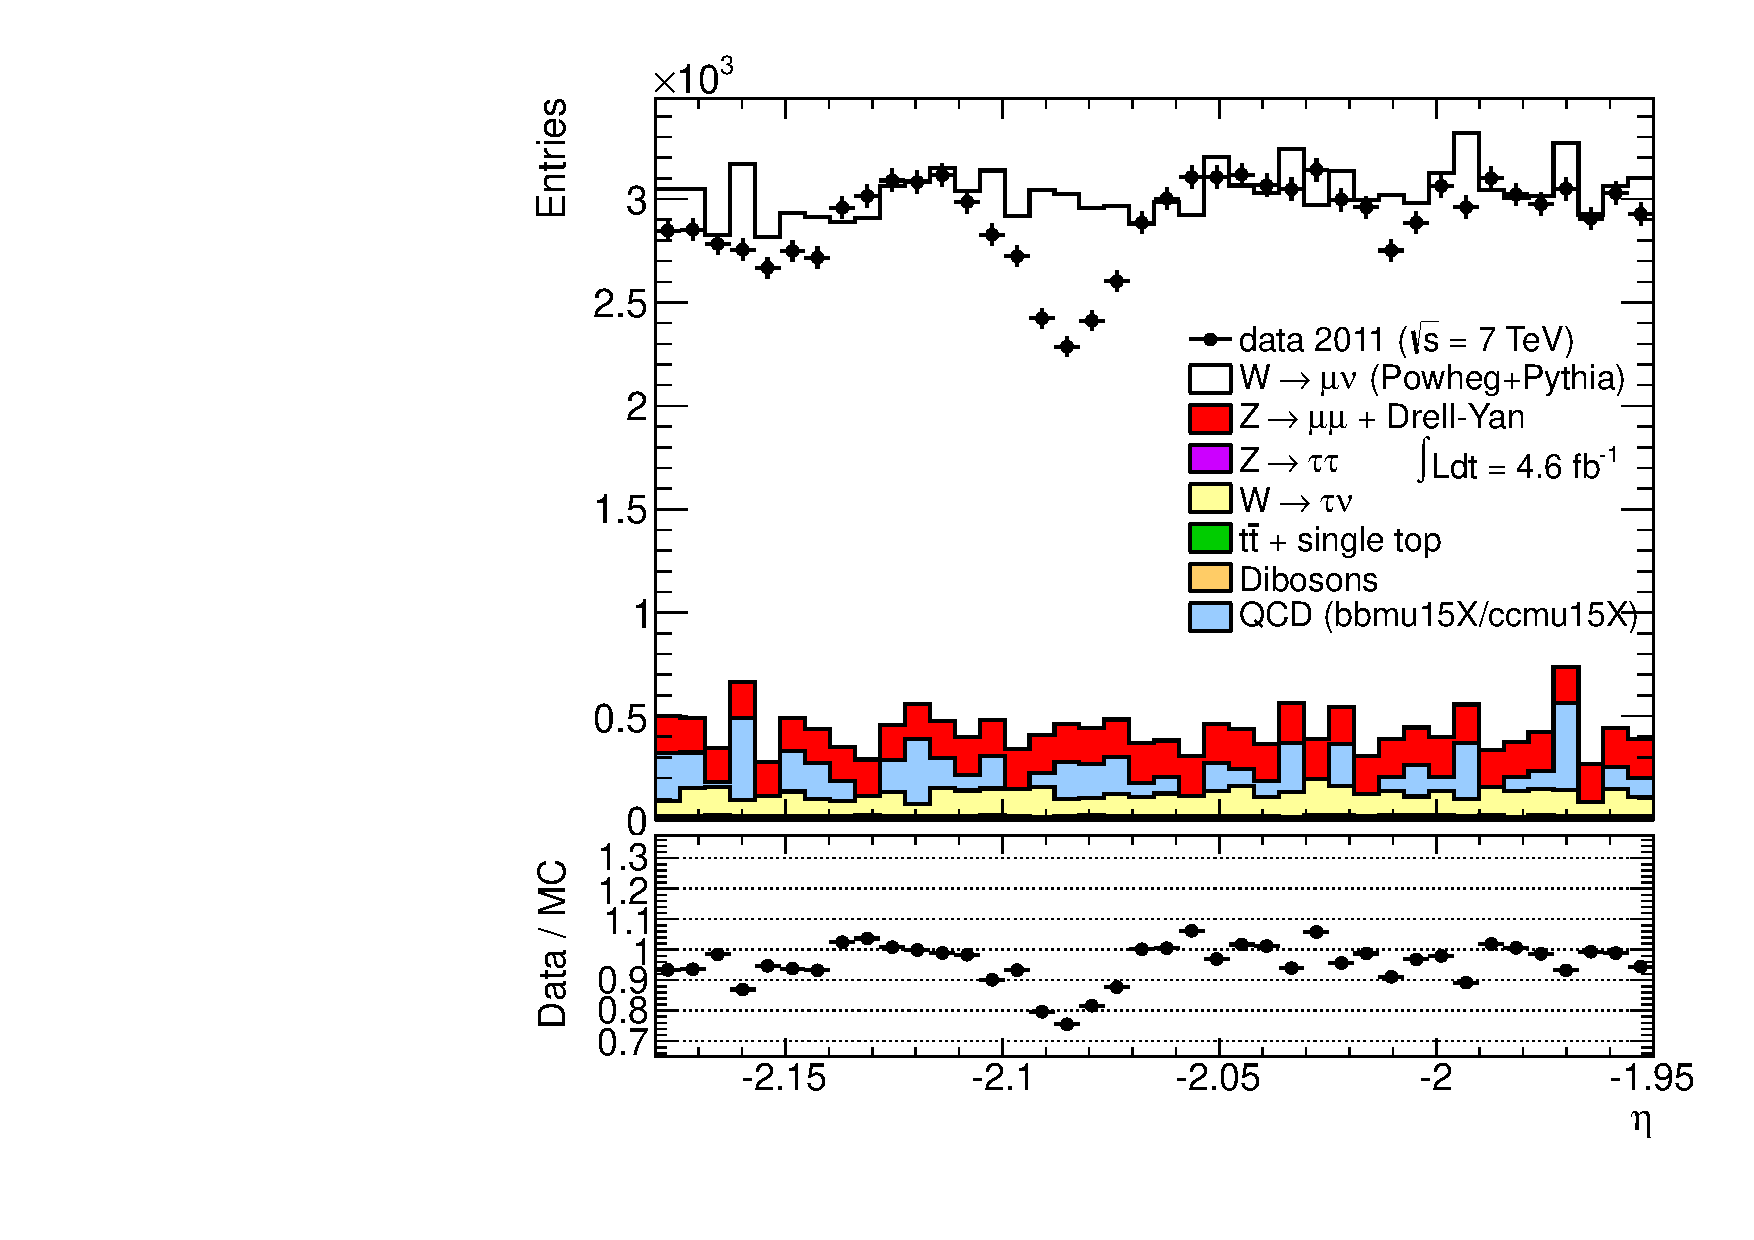
\includegraphics[width=0.66\textwidth]{dates/20130306/figures/both/Wpt2535_10_C_stack_l_eta_NEG} \\
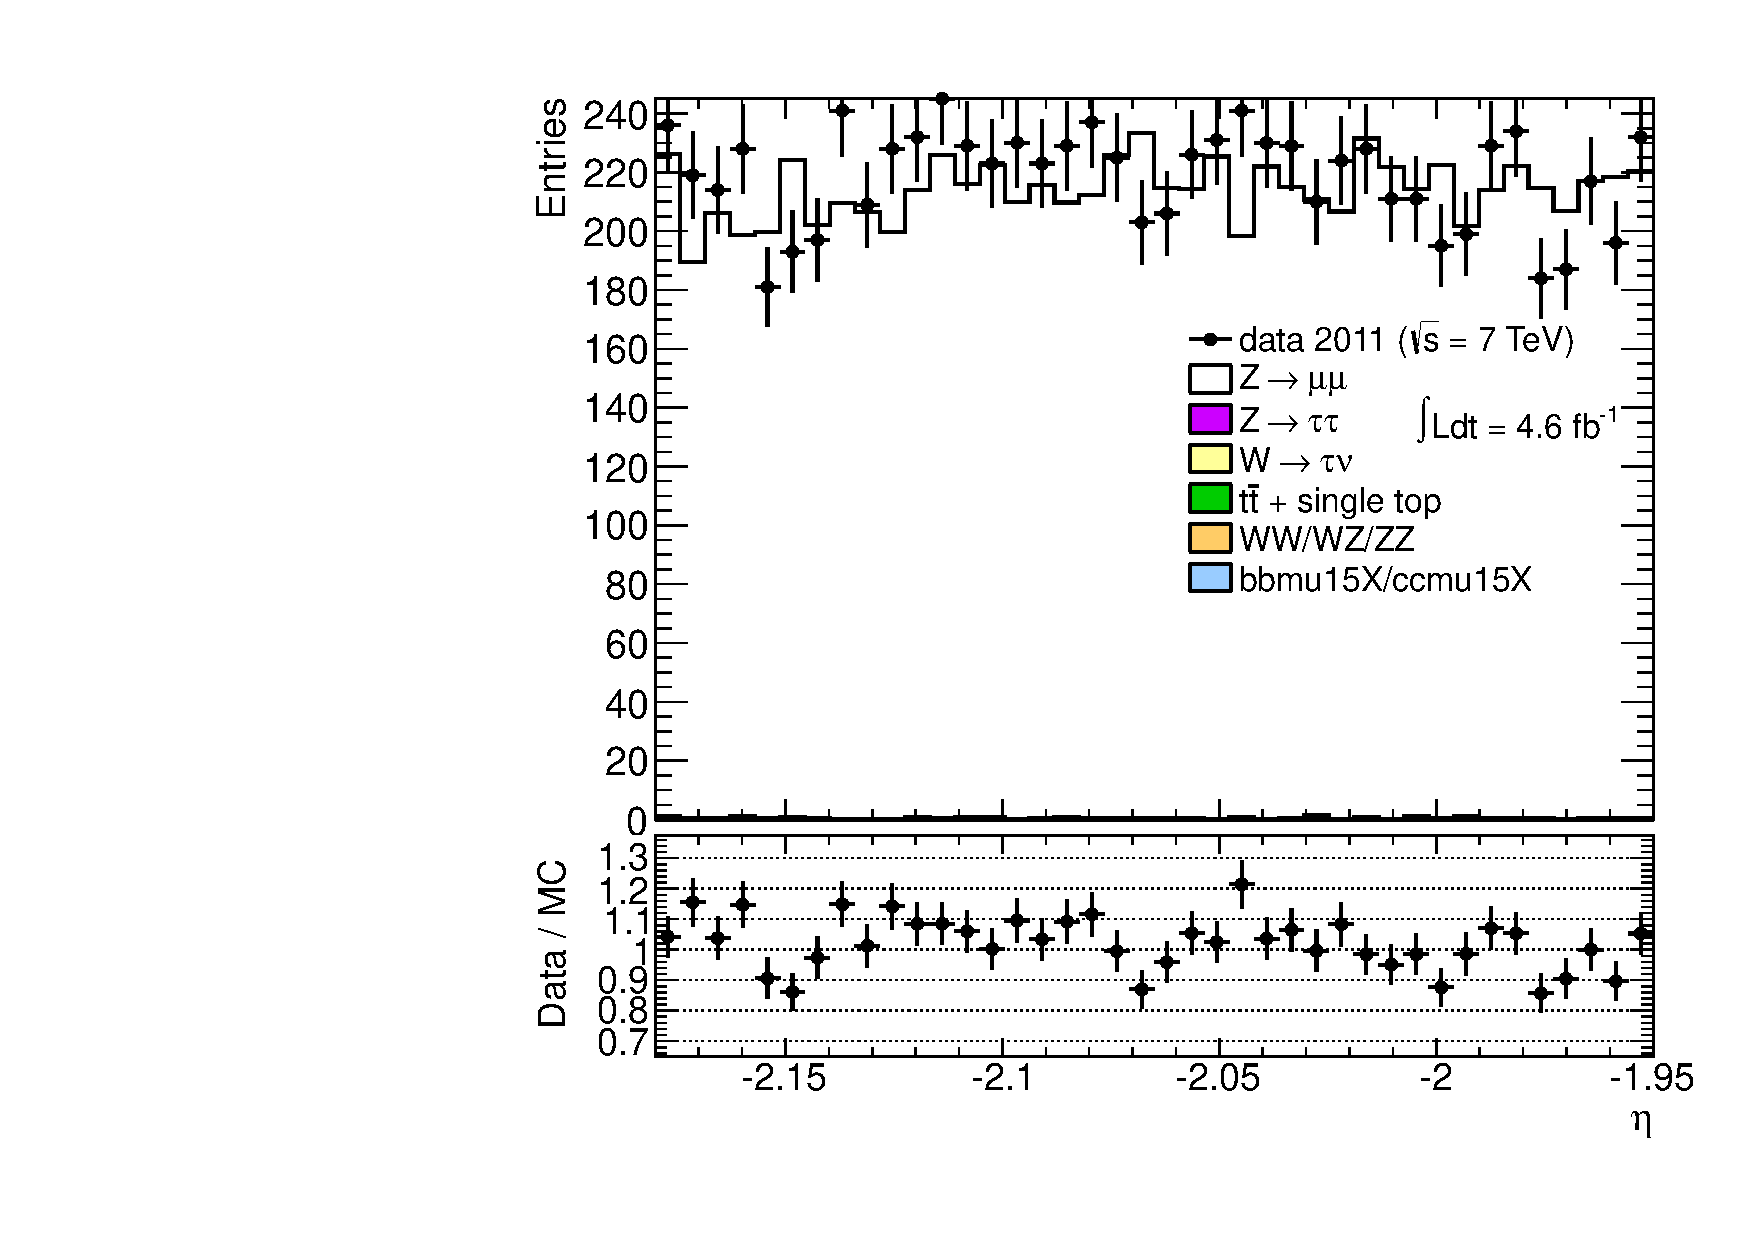
\includegraphics[width=0.66\textwidth]{dates/20130306/figures/both/Zpt2535_10_C_stack_lN_eta_ALL.pdf}
\column{.5\textwidth}
A-side $\mu^{-}$ (top: W; bottom: Z)
\centering
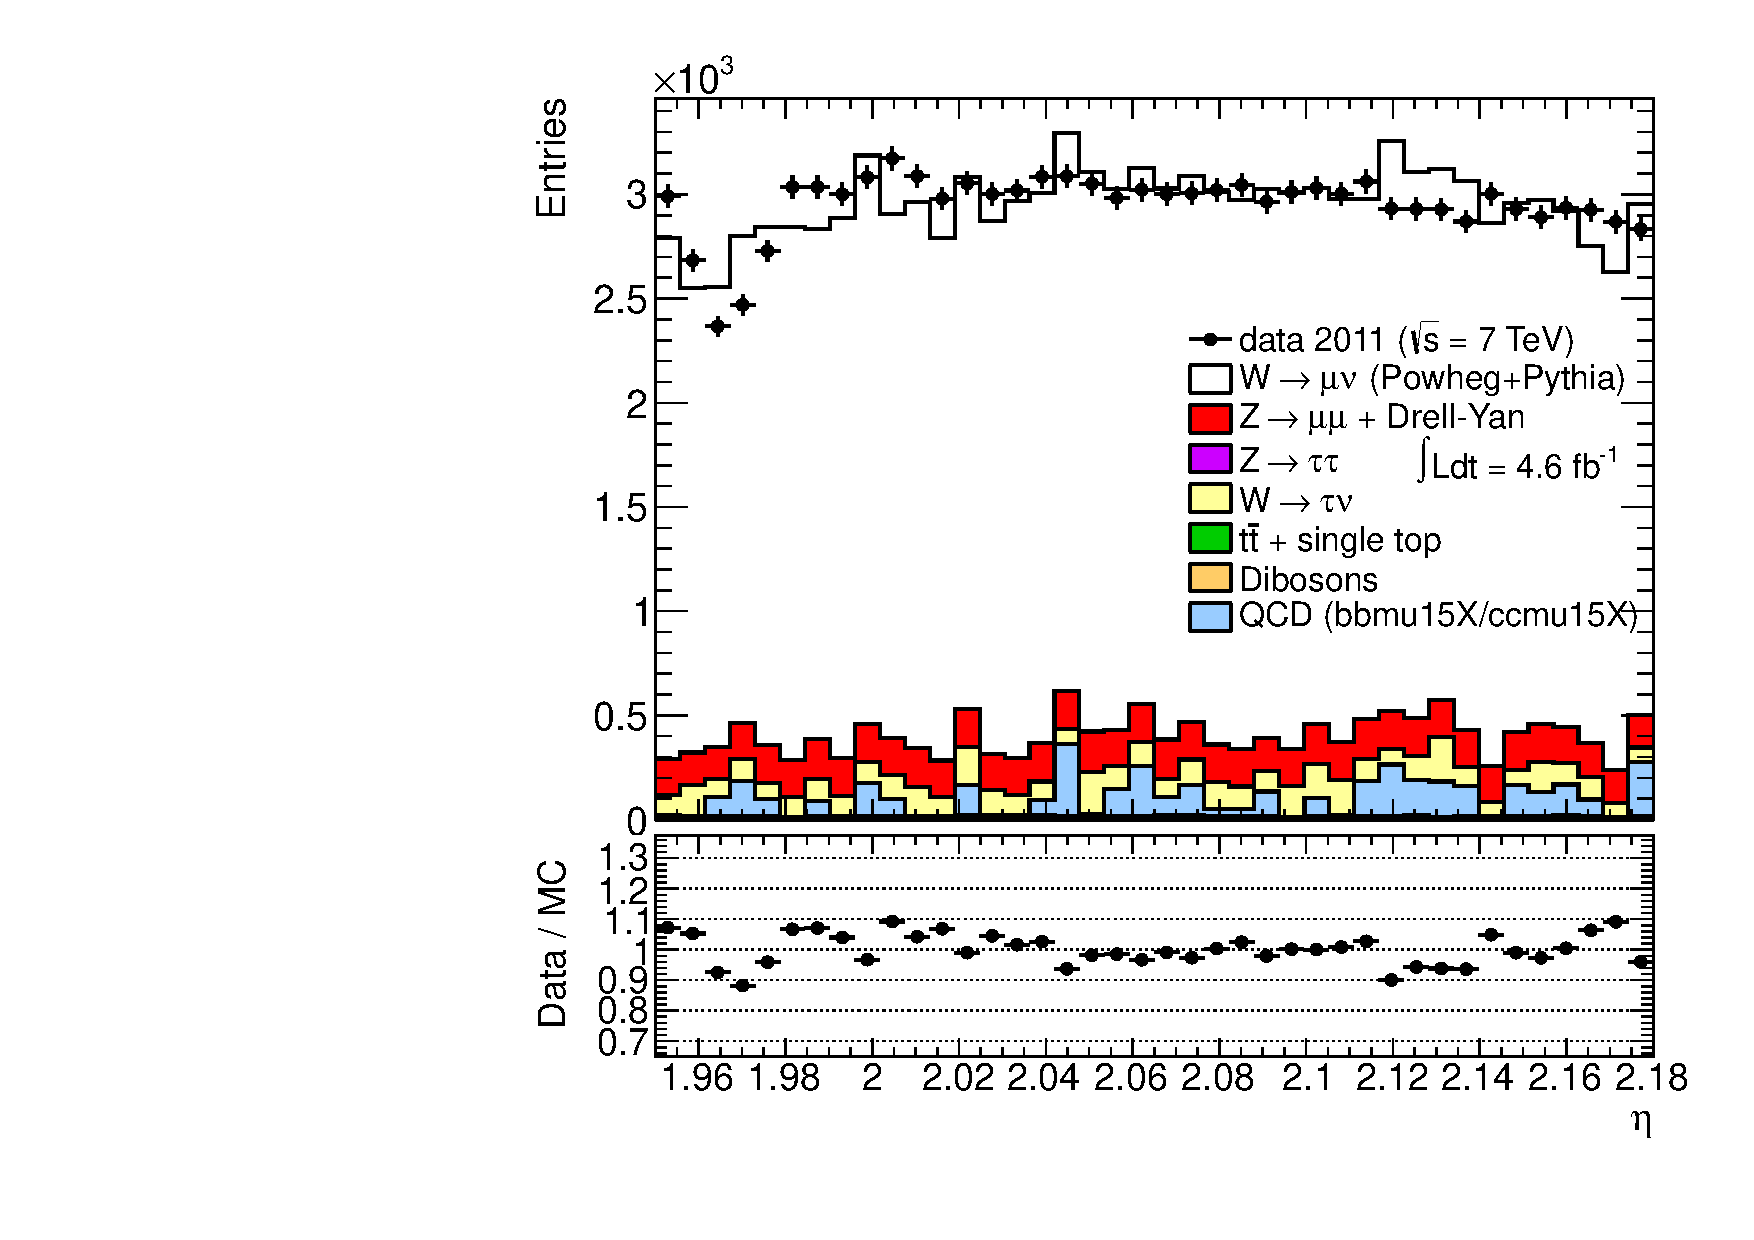
\includegraphics[width=0.66\textwidth]{dates/20130306/figures/both/Wpt2535_10_A_stack_l_eta_NEG} \\
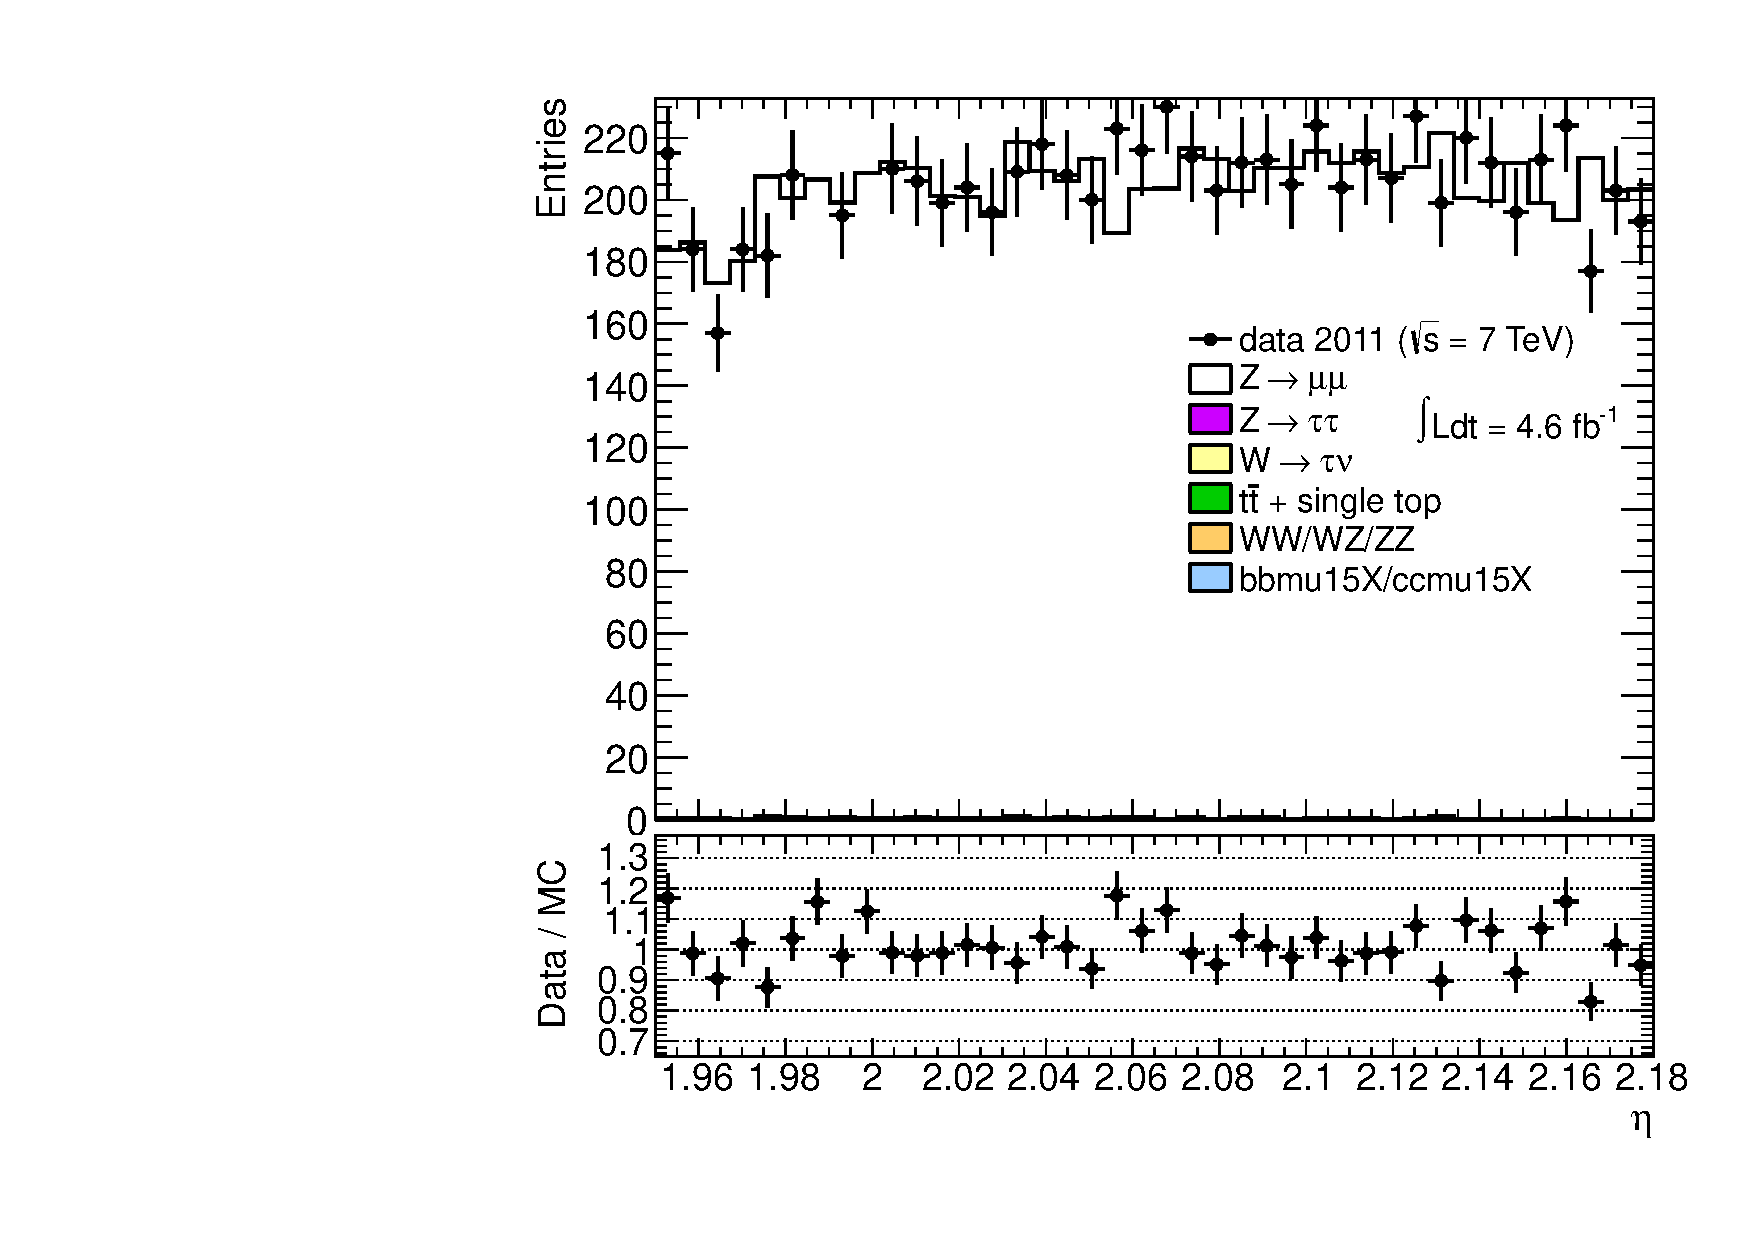
\includegraphics[width=0.66\textwidth]{dates/20130306/figures/both/Zpt2535_10_A_stack_lN_eta_ALL.pdf} 
\cole
}

\slide{ $\mu^{-}$: njets } {
Recall that in the A/C slide, there was a hint that $Z+jets$ may exhibit the dip. \\
(njets cut was added to break the phi correlation between the two Z muons).
Let's look at $\eta$ and $\phi$ with $njets>=1$ for both W and Z muons.
}
\slide{ $\mu^{-}$: njets } {
\colb[T]
\column{.5\textwidth}
C-side $\mu^{-}$ (top: W; bottom: Z)
\centering
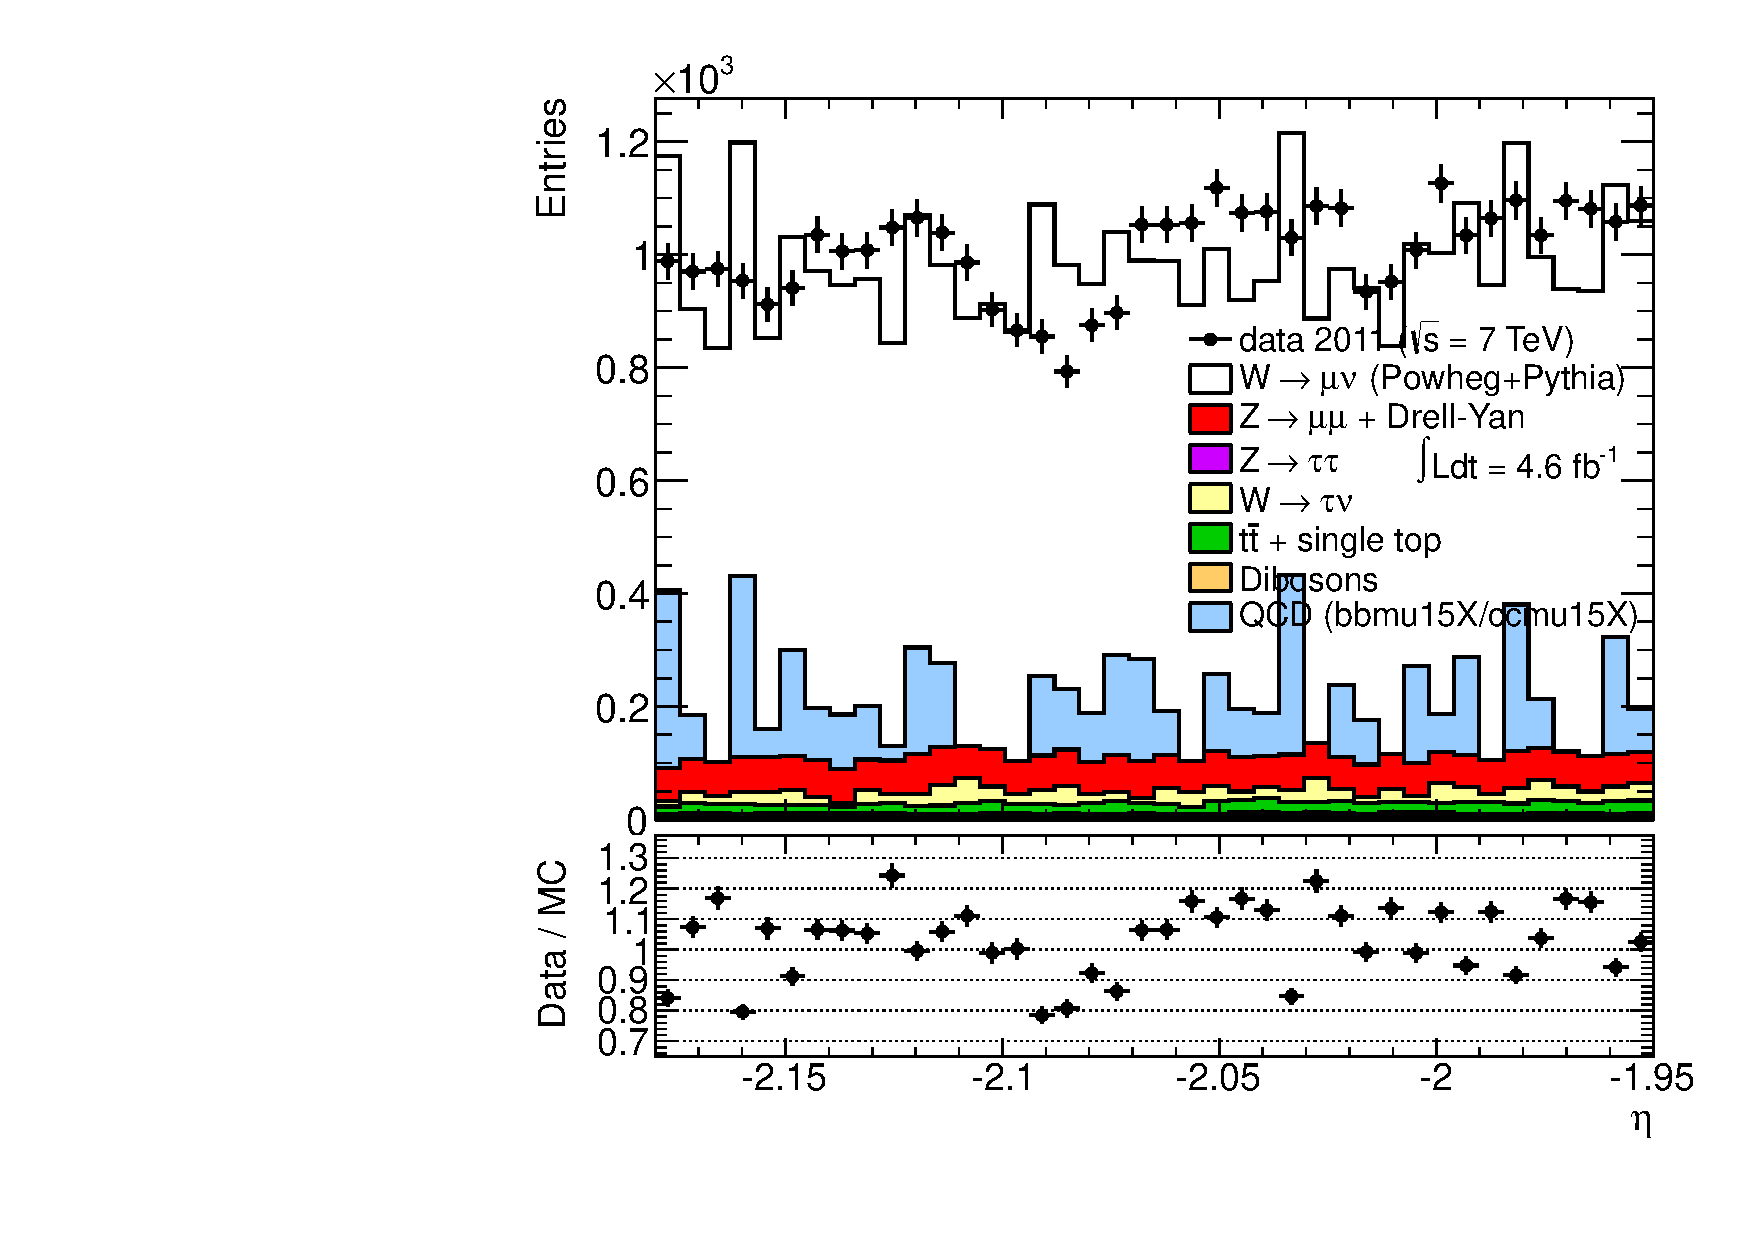
\includegraphics[width=0.66\textwidth]{dates/20130306/figures/both/Wnjets_10_C_stack_l_eta_NEG} \\
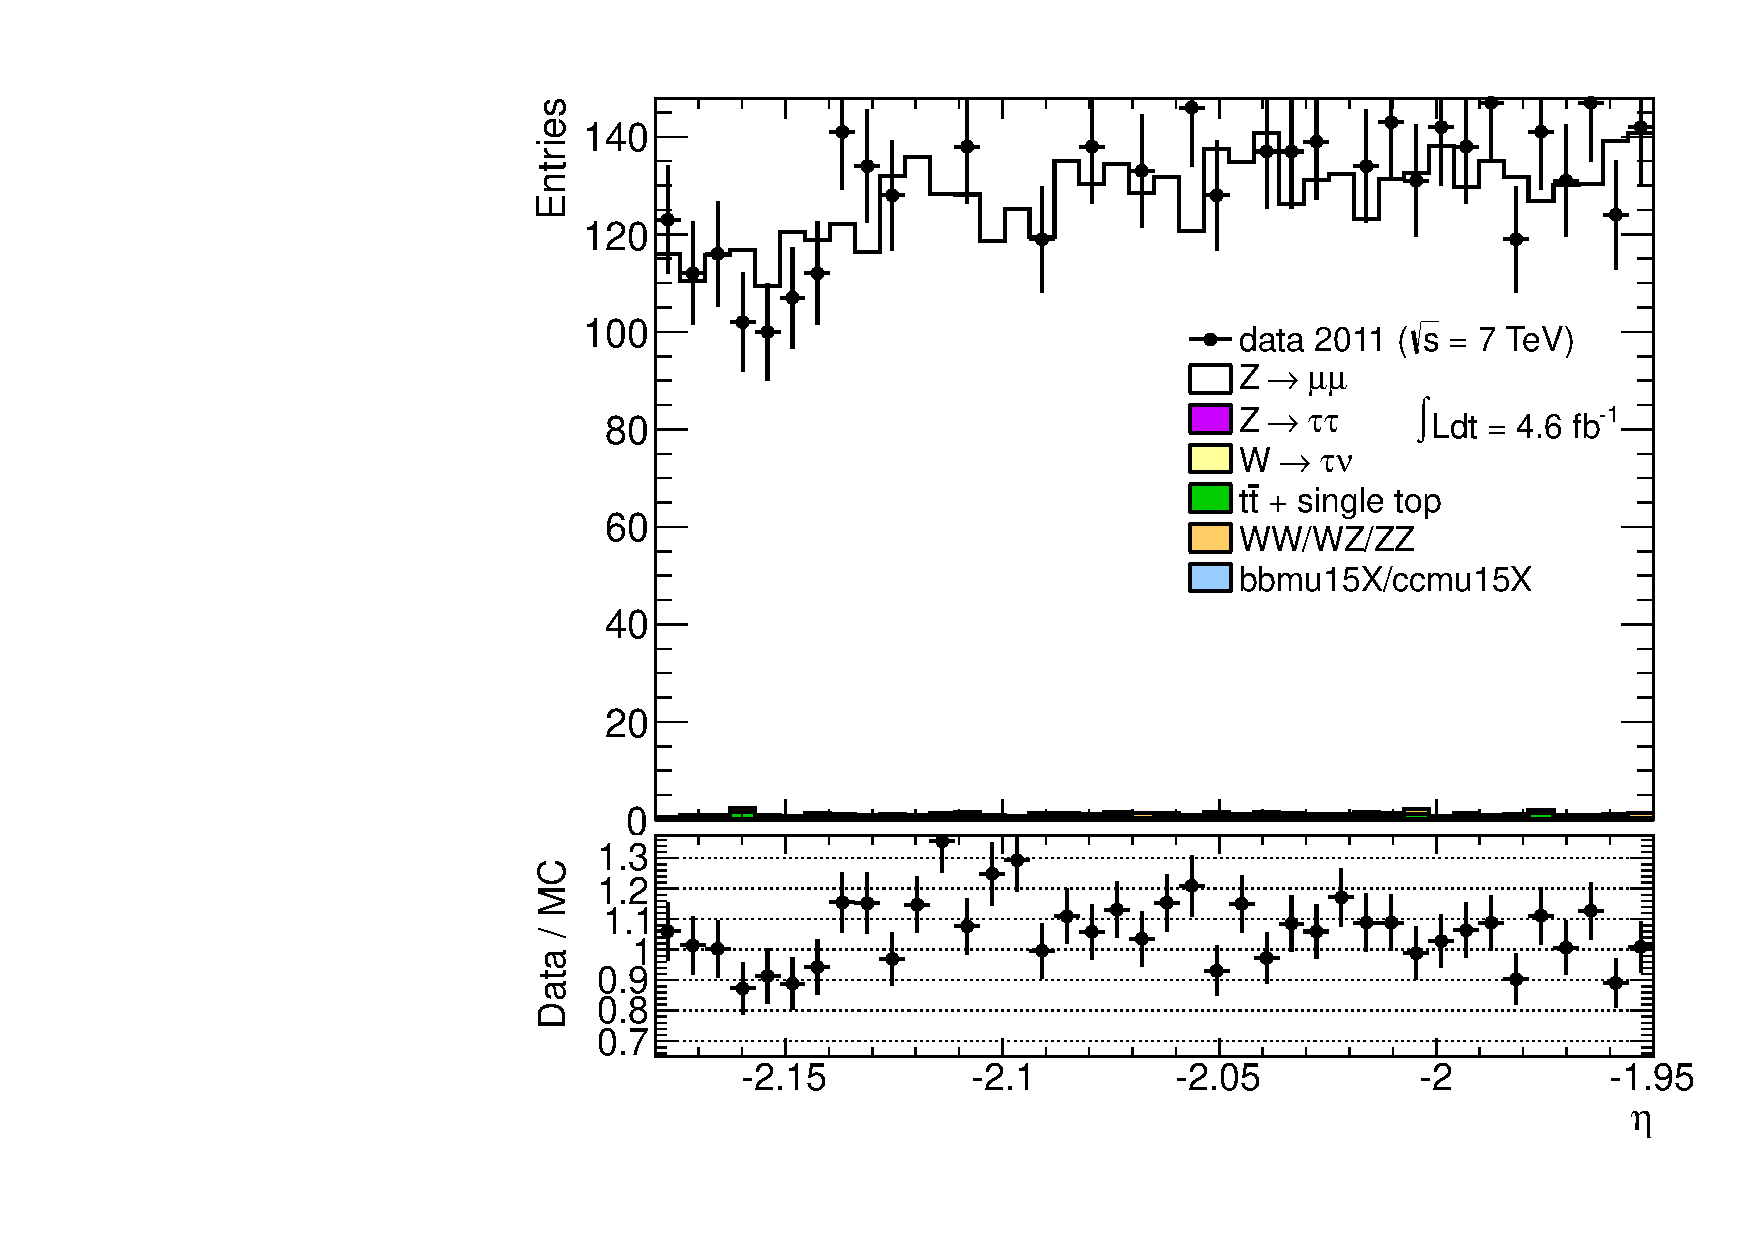
\includegraphics[width=0.66\textwidth]{dates/20130306/figures/both/Znjets_10_C_stack_lN_eta_ALL.pdf}
\column{.5\textwidth}
A-side $\mu^{-}$ (top: W; bottom: Z)
\centering
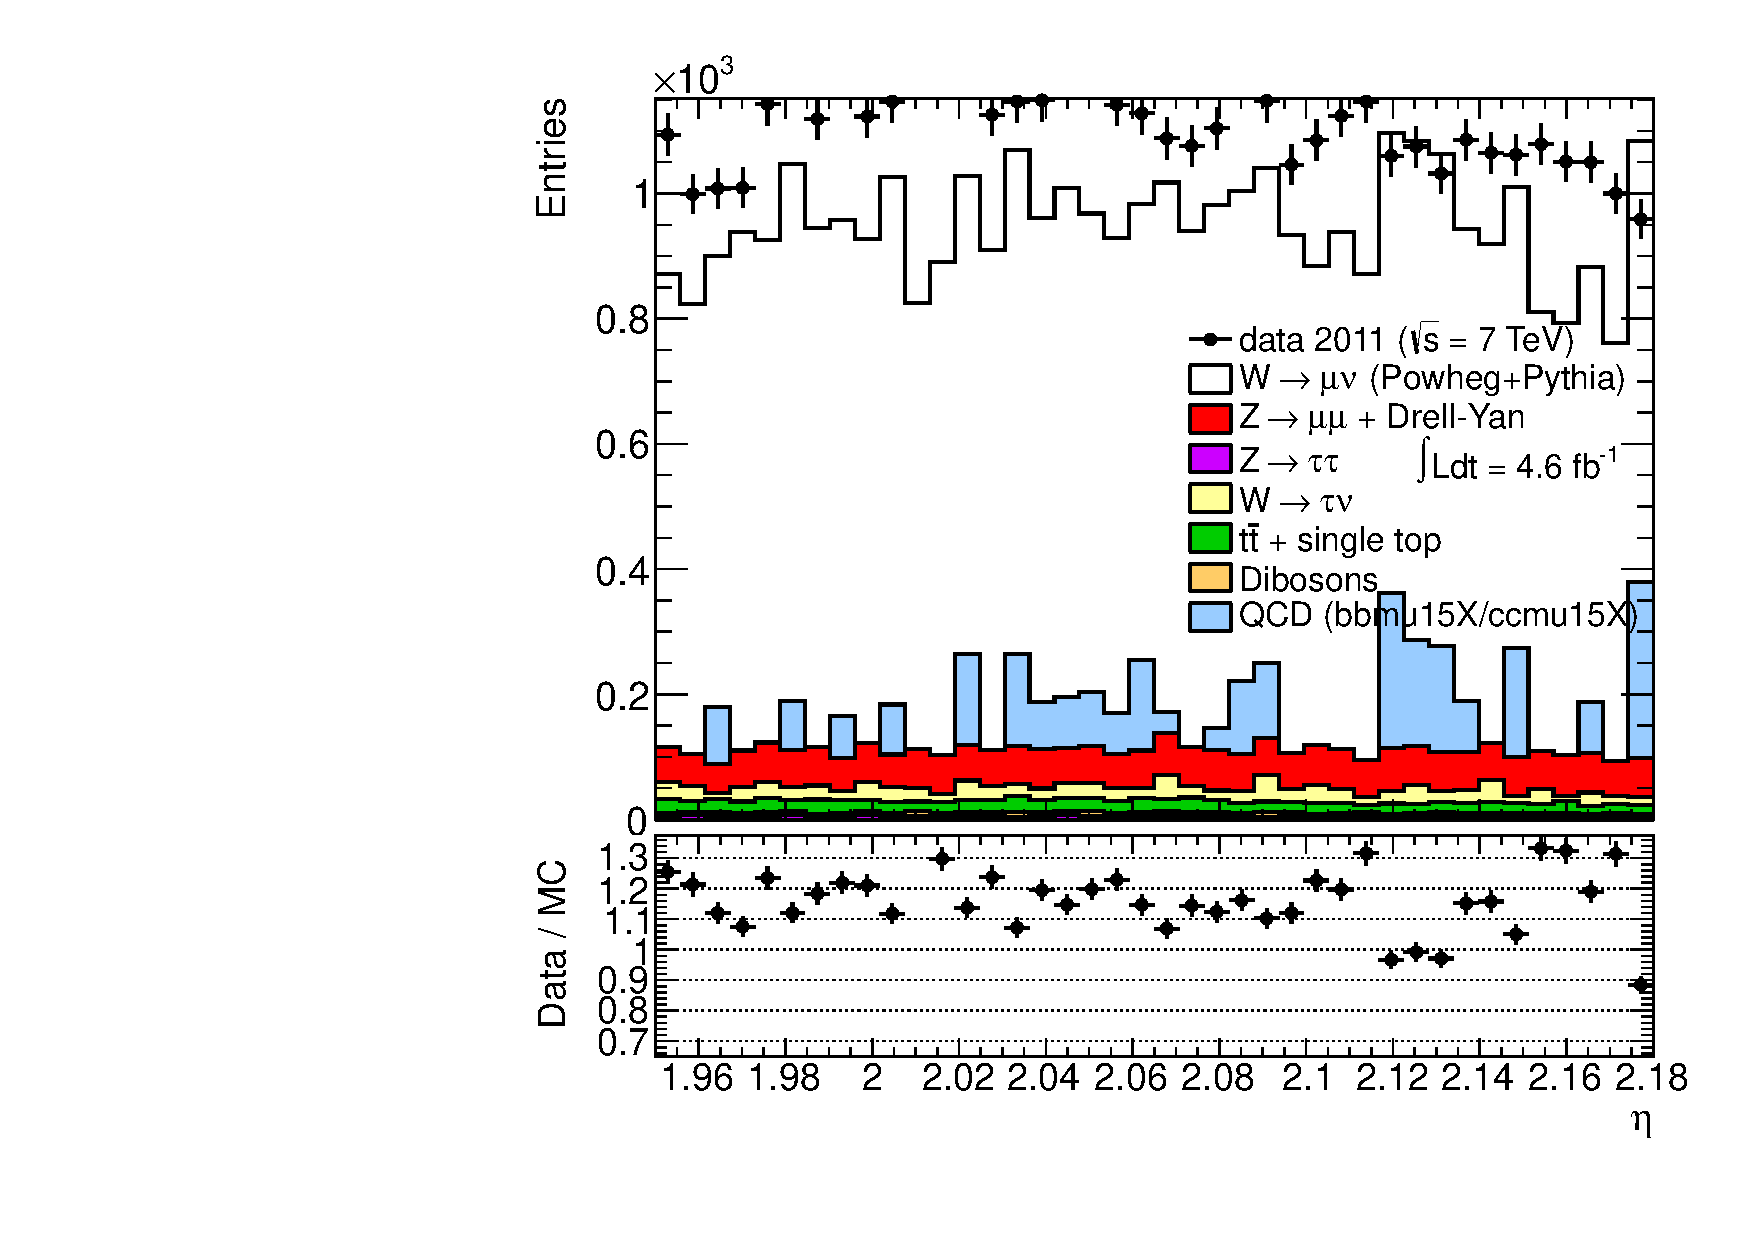
\includegraphics[width=0.66\textwidth]{dates/20130306/figures/both/Wnjets_10_A_stack_l_eta_NEG} \\
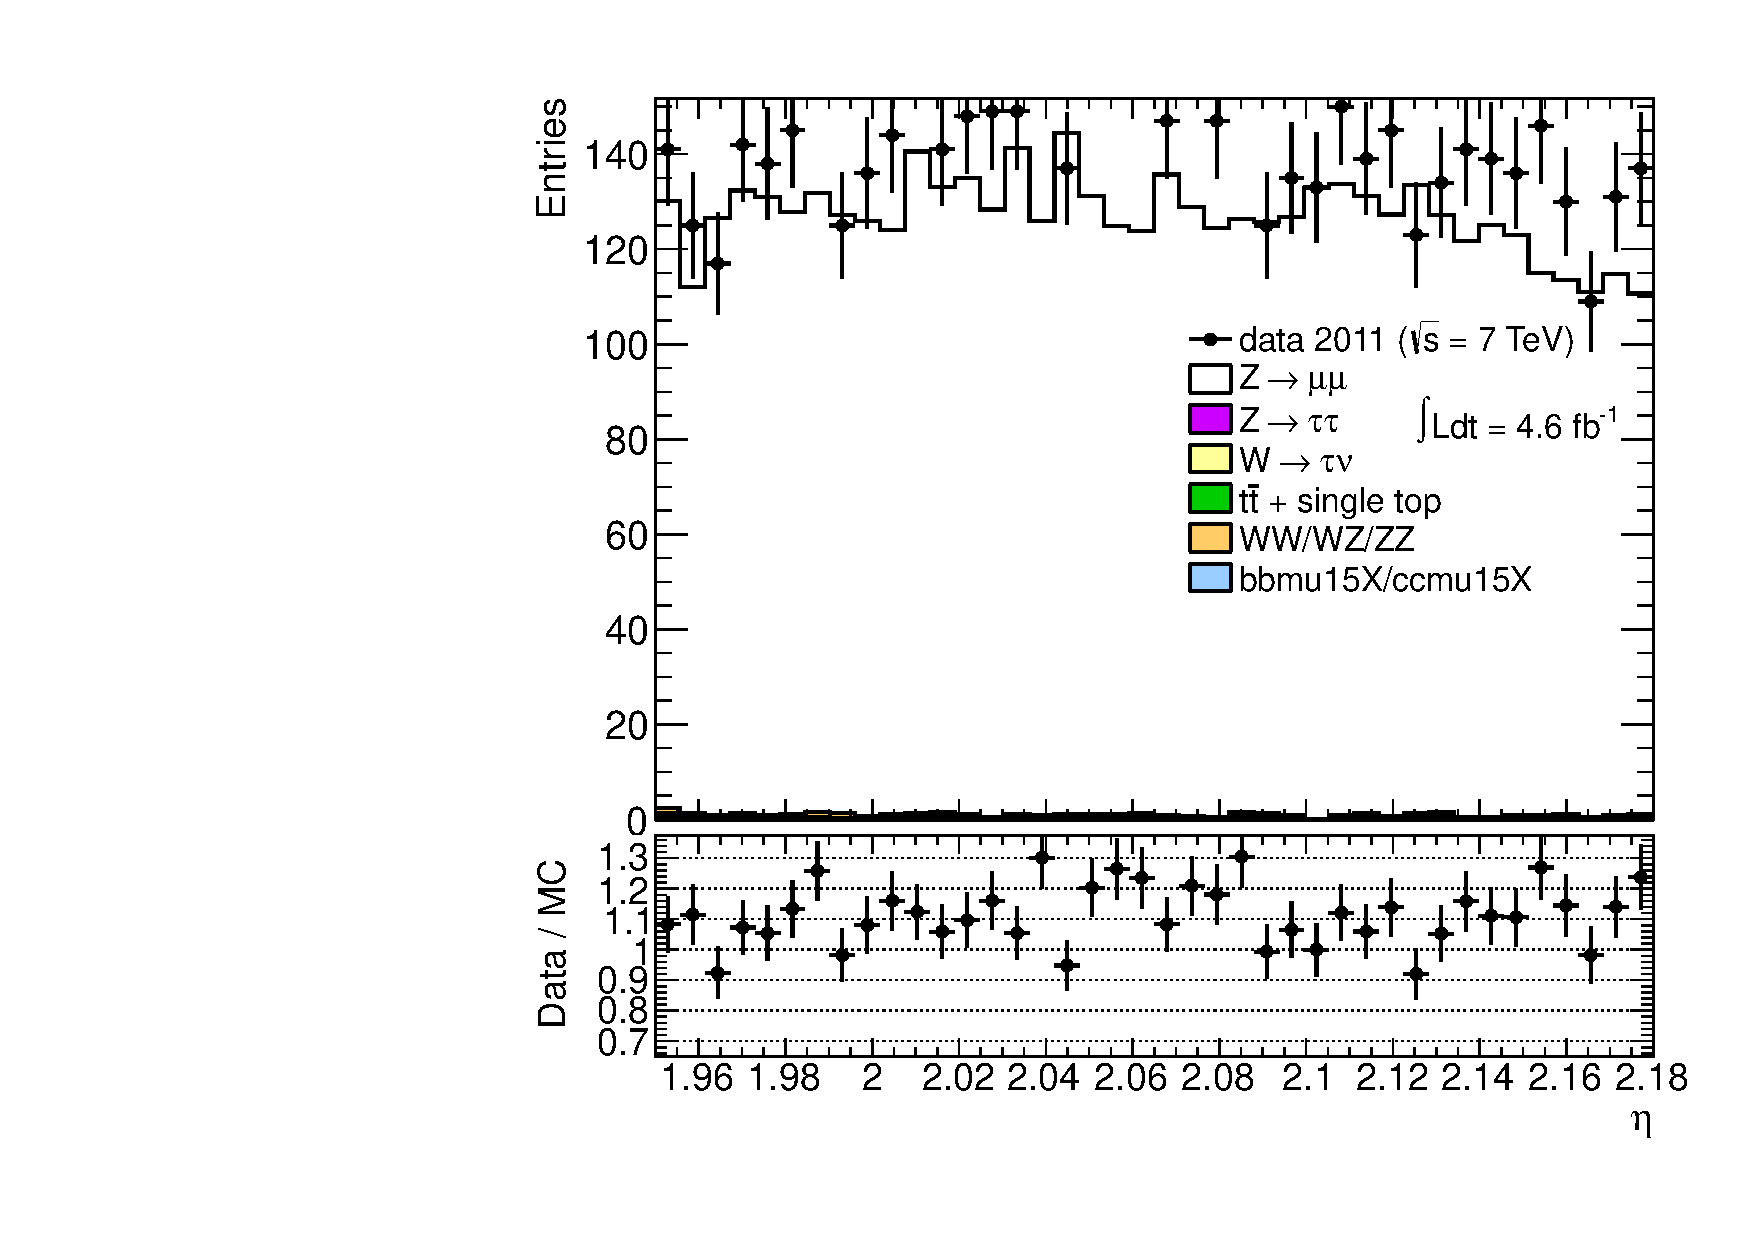
\includegraphics[width=0.66\textwidth]{dates/20130306/figures/both/Znjets_10_A_stack_lN_eta_ALL.pdf} 
\cole
}

\slide{ $\mu^{-}$: tag in barrel } {
Another way to break the Z muon correlations: \\
Force the other (tag) muon to be in the \red{barrel}.
}
\slide{ $\mu^{-}$: tag in barrel } {
\colb[T]
\column{.5\textwidth}
C-side $\mu^{-}$ (top: W; bottom: Z)
\centering
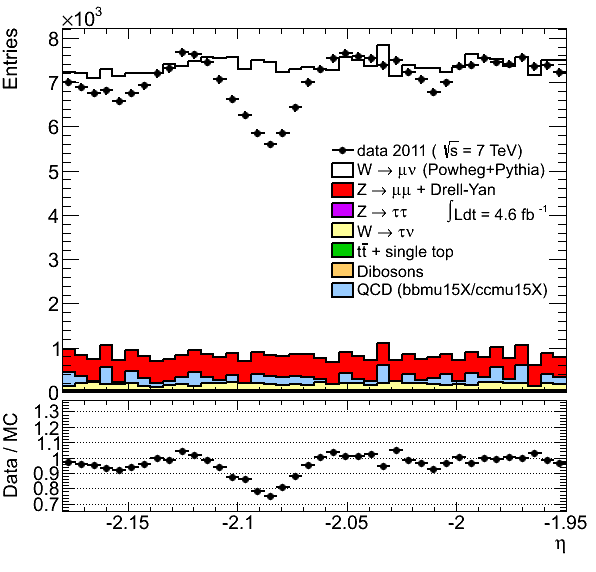
\includegraphics[width=0.66\textwidth]{dates/20130306/figures/both/W_10_C_stack_l_eta_NEG} \\
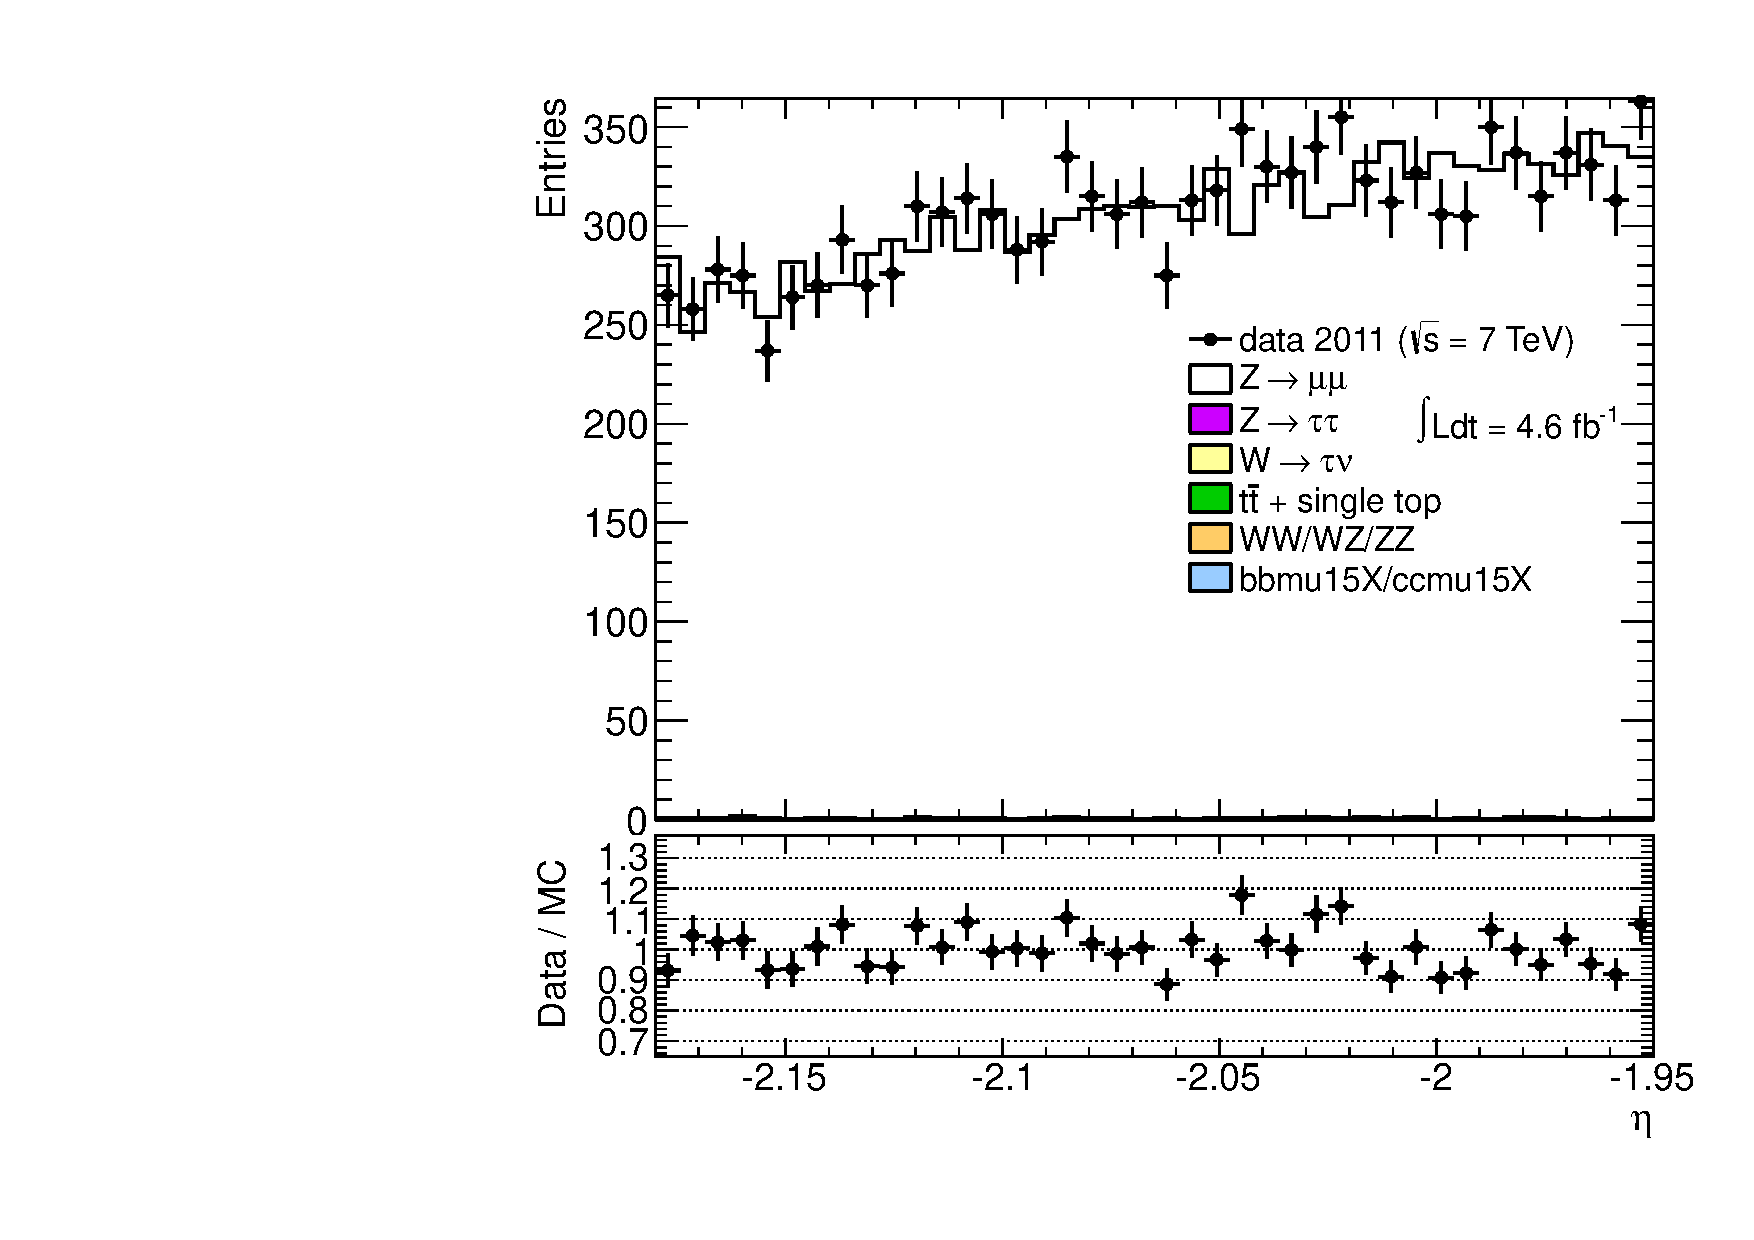
\includegraphics[width=0.66\textwidth]{dates/20130306/figures/both/ZlObarrel_10_C_stack_lN_eta_ALL.pdf}
\column{.5\textwidth}
A-side $\mu^{-}$ (top: W; bottom: Z)
\centering
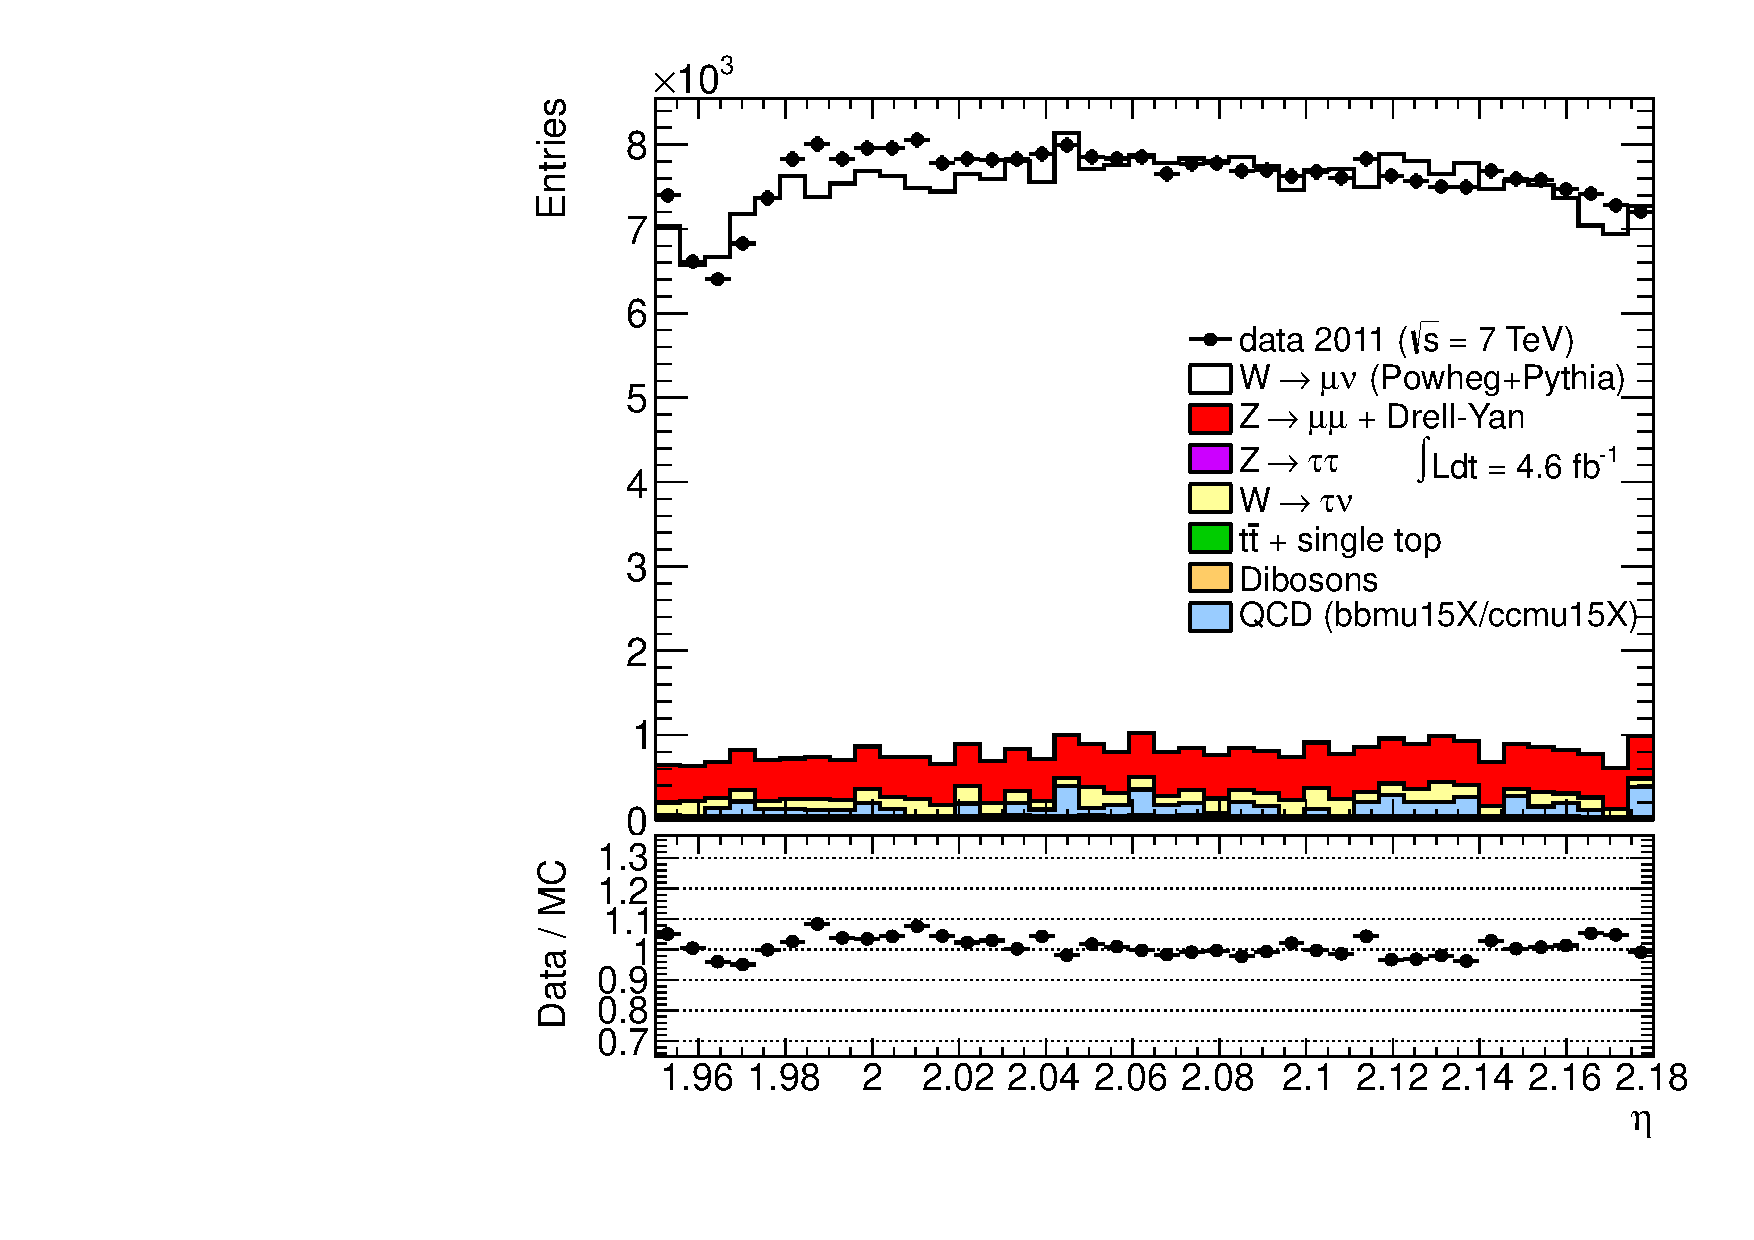
\includegraphics[width=0.66\textwidth]{dates/20130306/figures/both/W_10_A_stack_l_eta_NEG} \\
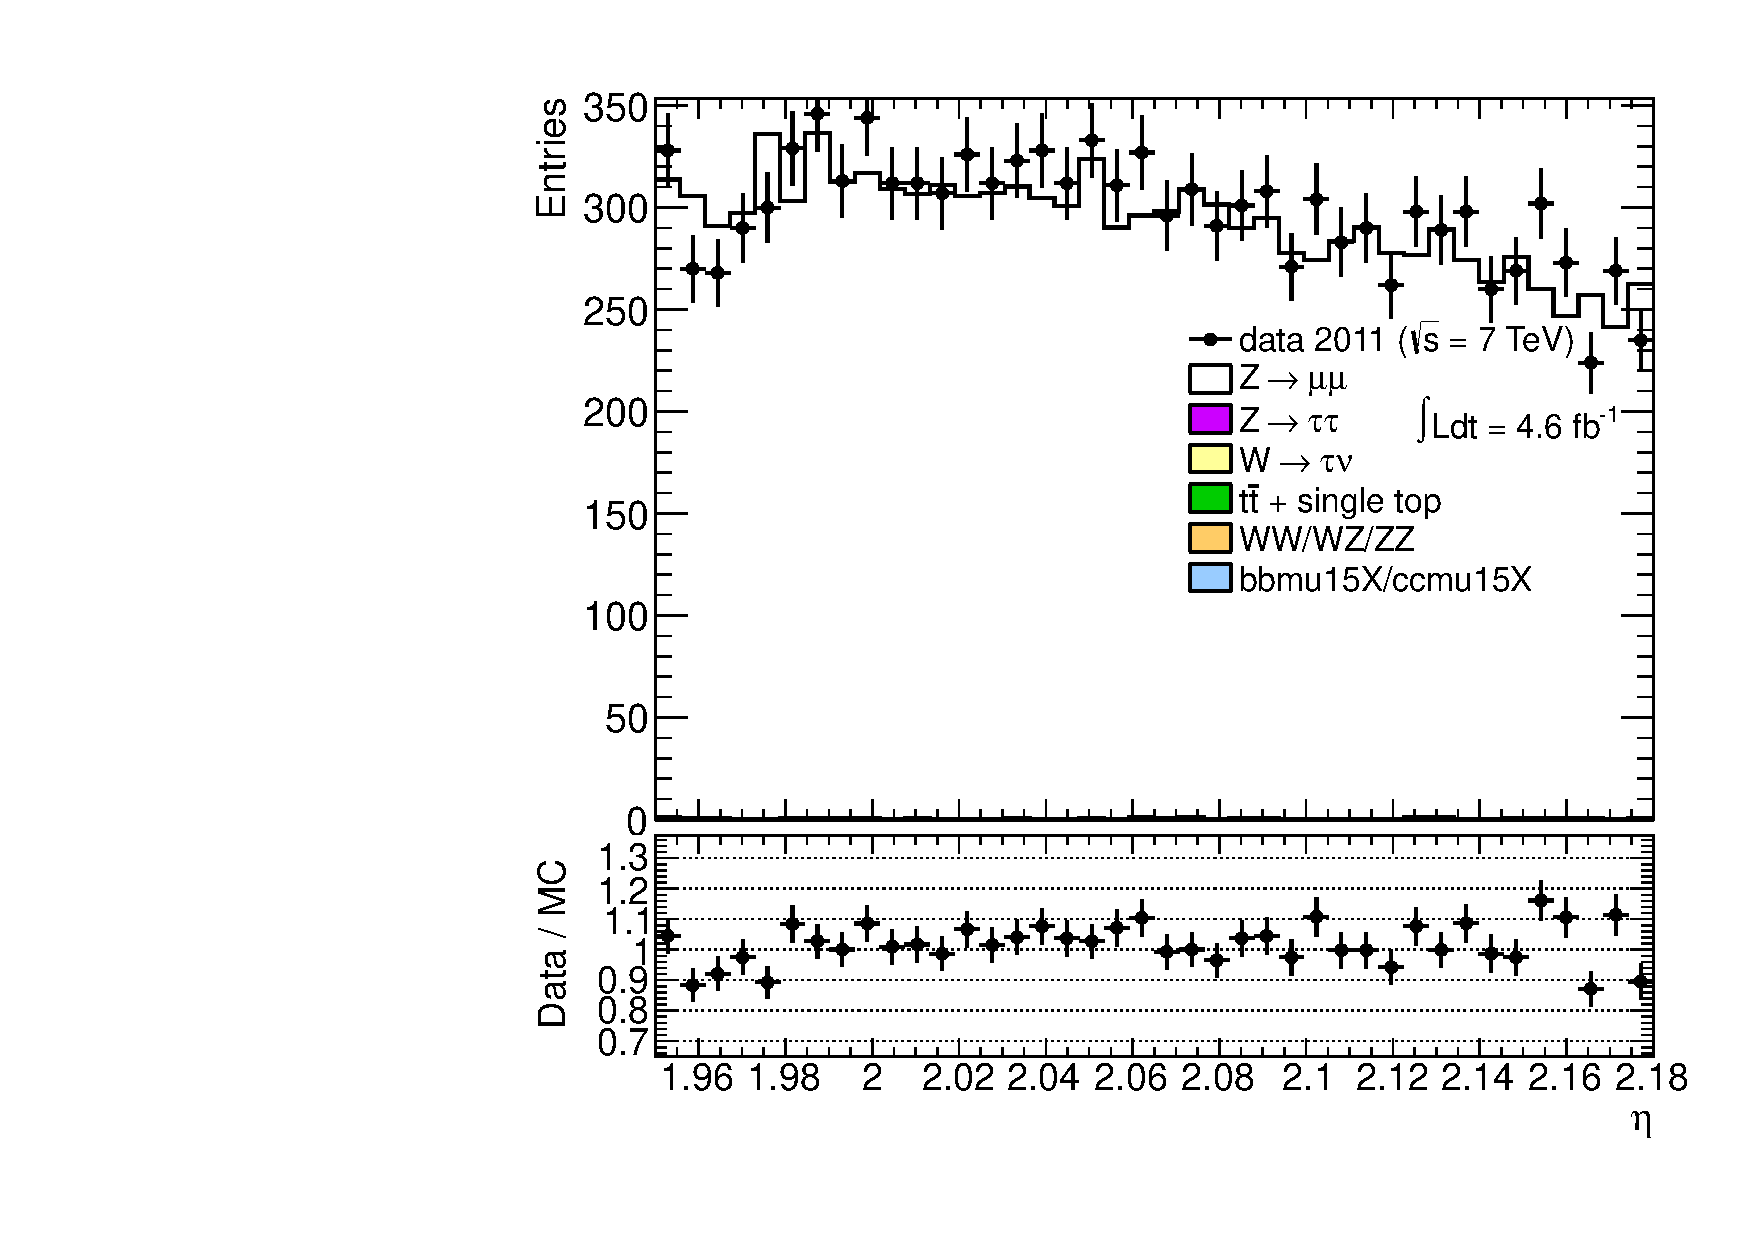
\includegraphics[width=0.66\textwidth]{dates/20130306/figures/both/ZlObarrel_10_A_stack_lN_eta_ALL.pdf} 
\cole
}

\slide{ $\mu^{-}$: tag in endcap } {
For completeness, let's force the other (tag) muon to be in the \red{endcap}.
}
\slide{ $\mu^{-}$: tag in endcap } {
\colb[T]
\column{.5\textwidth}
C-side $\mu^{-}$ (top: W; bottom: Z)
\centering
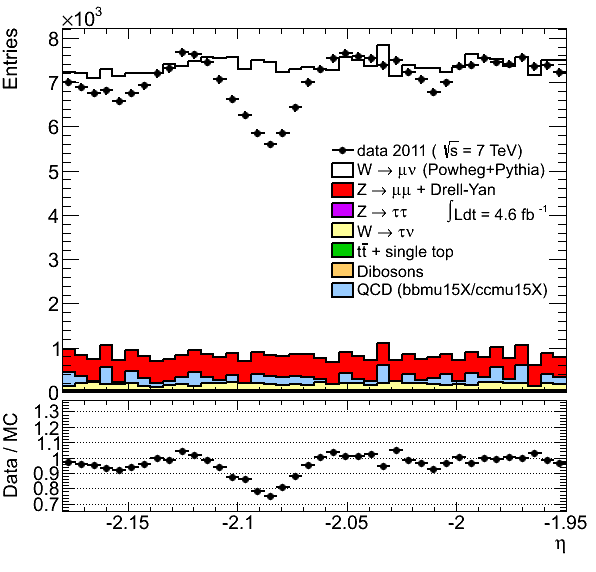
\includegraphics[width=0.66\textwidth]{dates/20130306/figures/both/W_10_C_stack_l_eta_NEG} \\
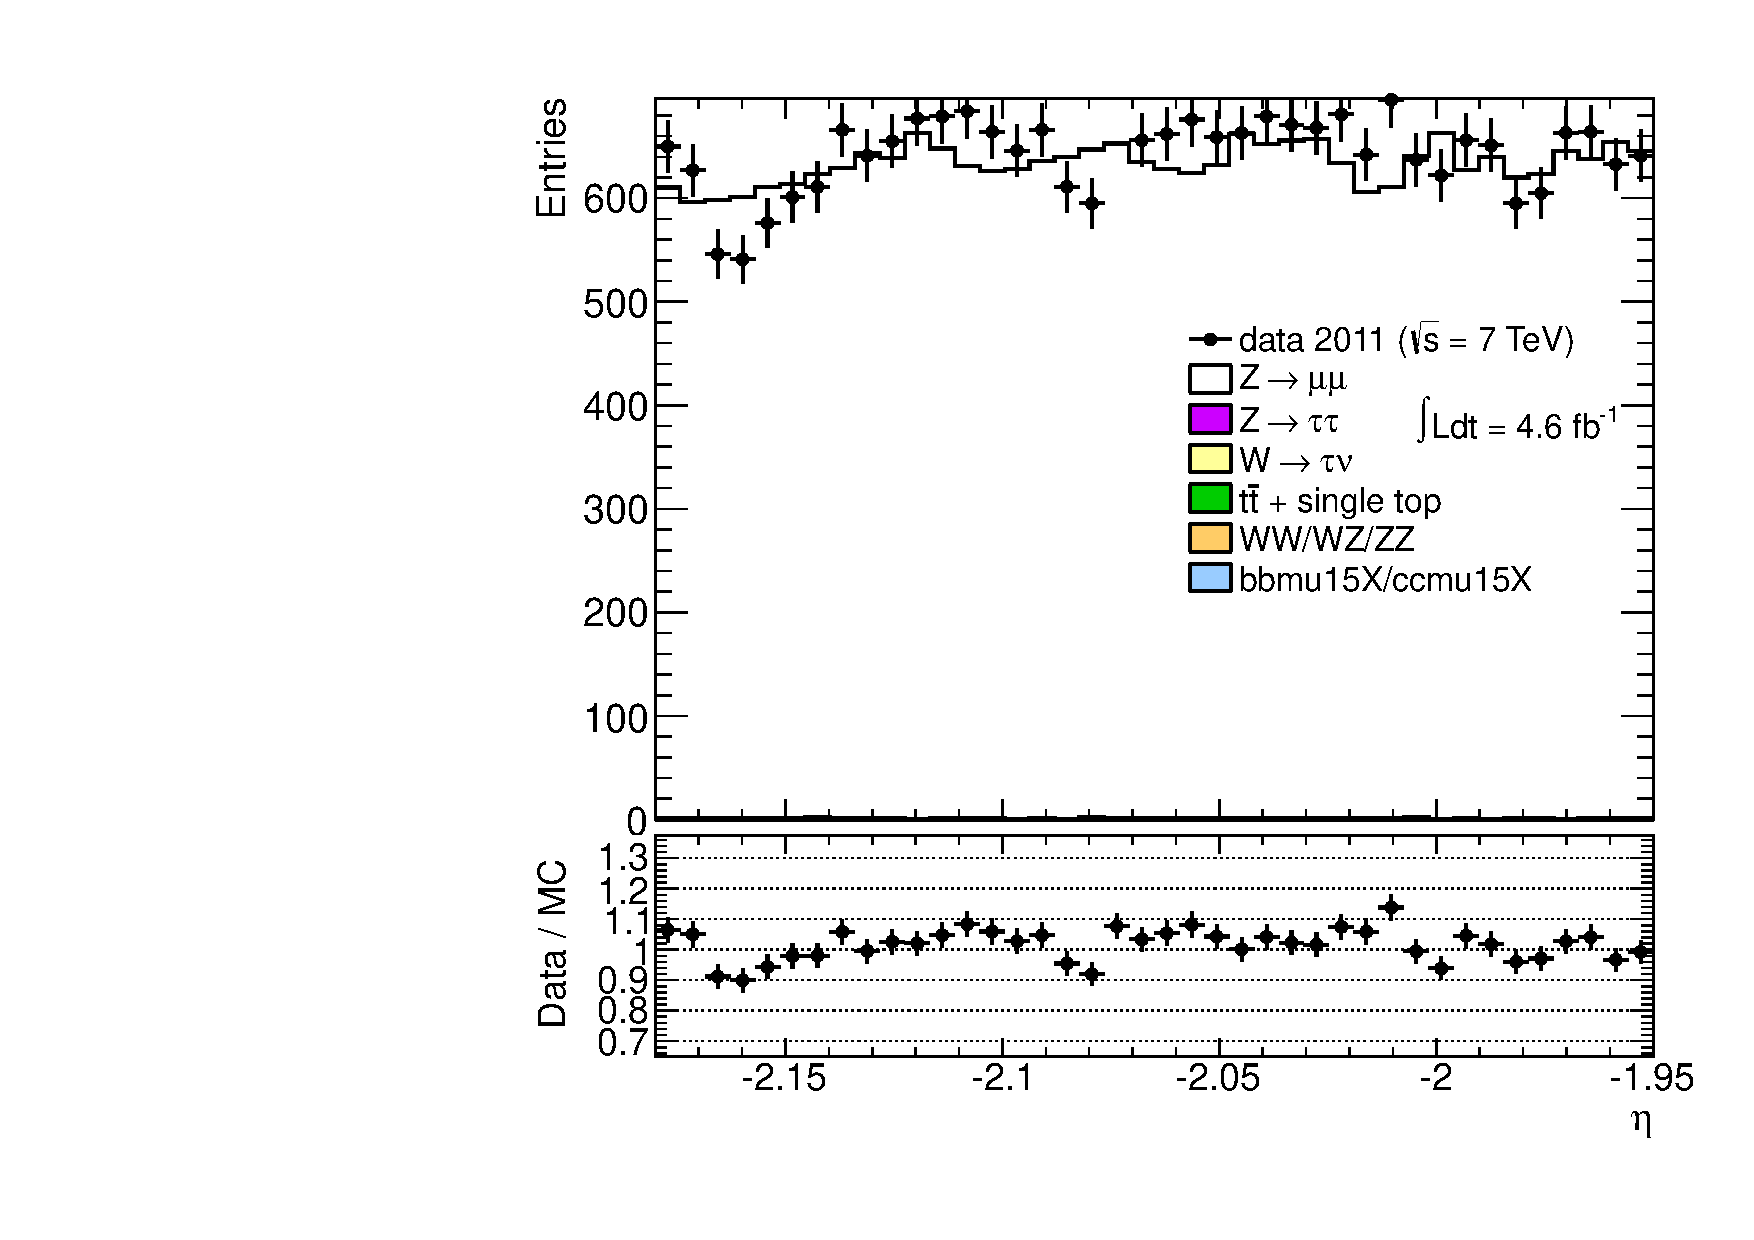
\includegraphics[width=0.66\textwidth]{dates/20130306/figures/both/ZlOendcap_10_C_stack_lN_eta_ALL.pdf}
\column{.5\textwidth}
A-side $\mu^{-}$ (top: W; bottom: Z)
\centering
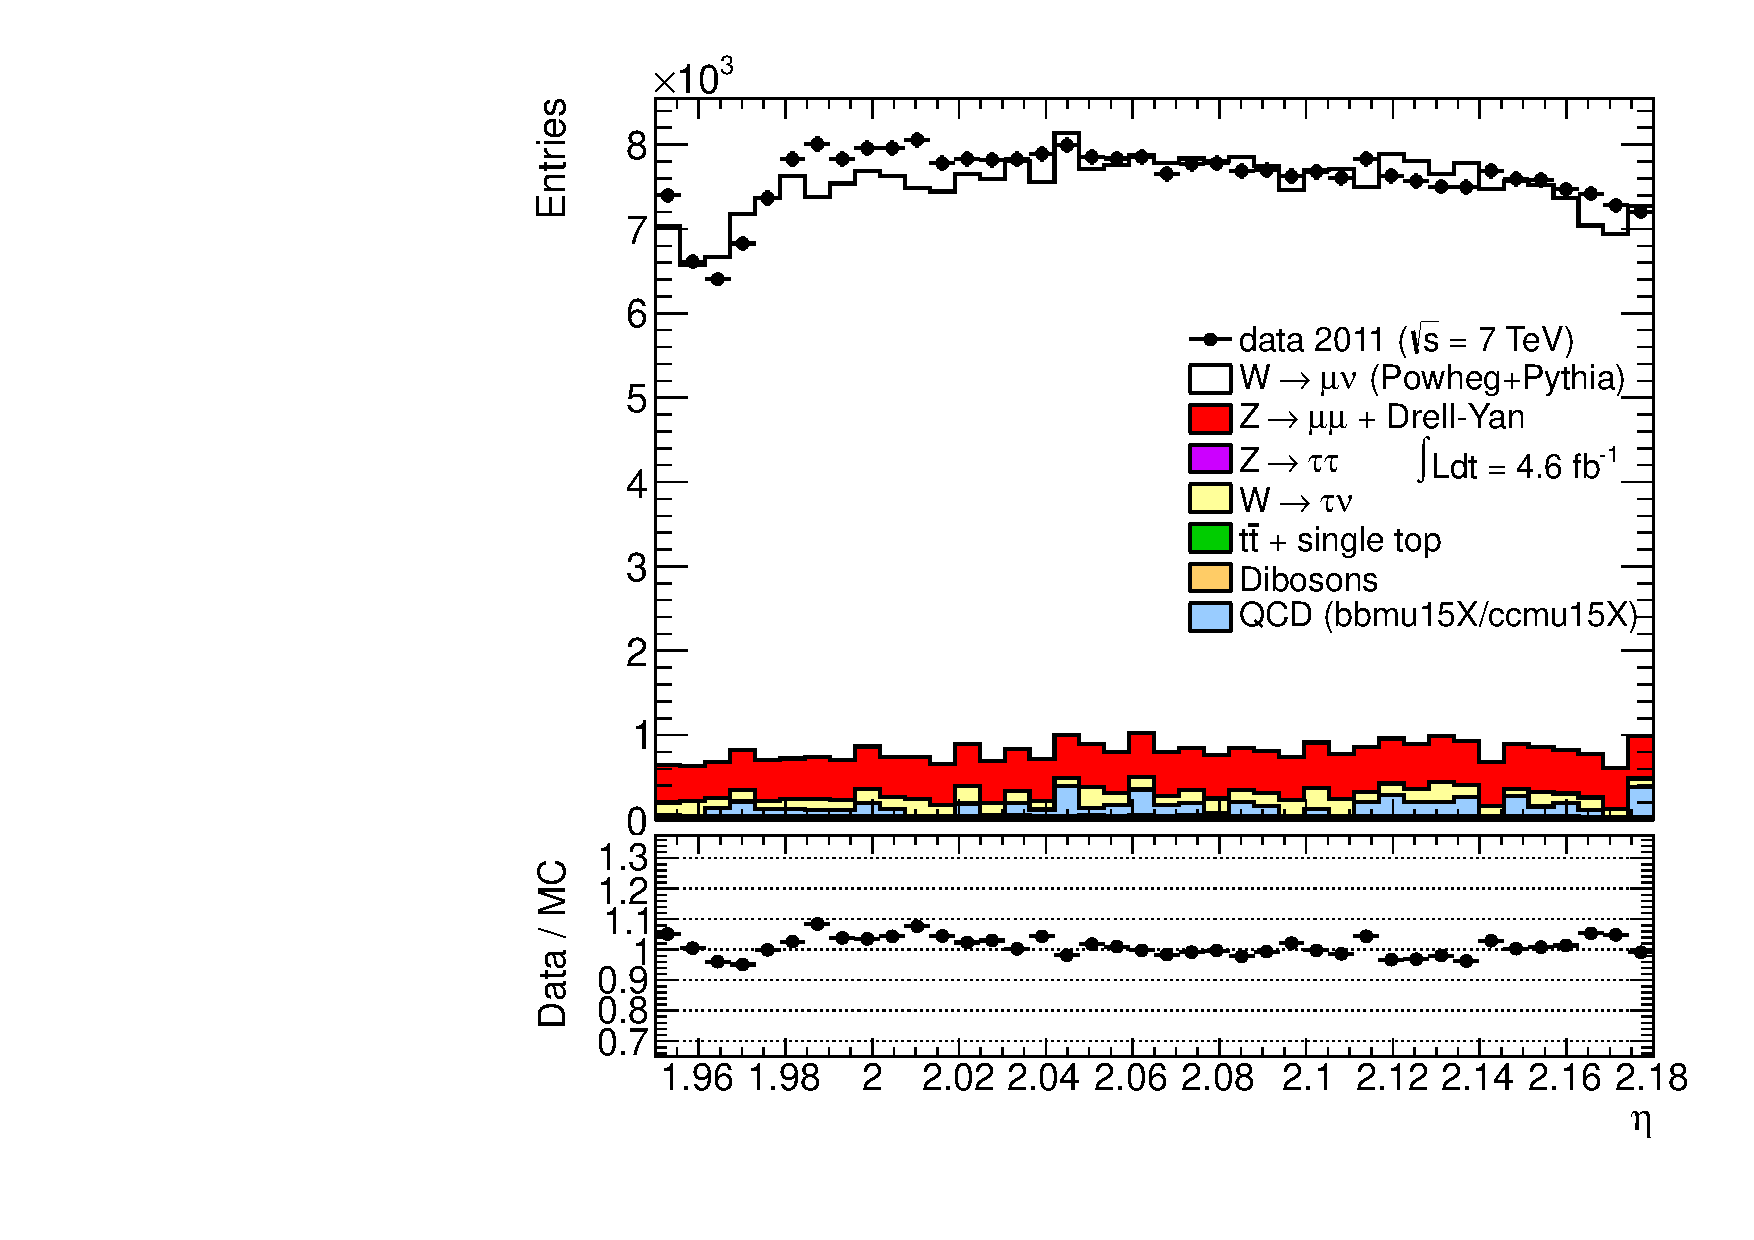
\includegraphics[width=0.66\textwidth]{dates/20130306/figures/both/W_10_A_stack_l_eta_NEG} \\
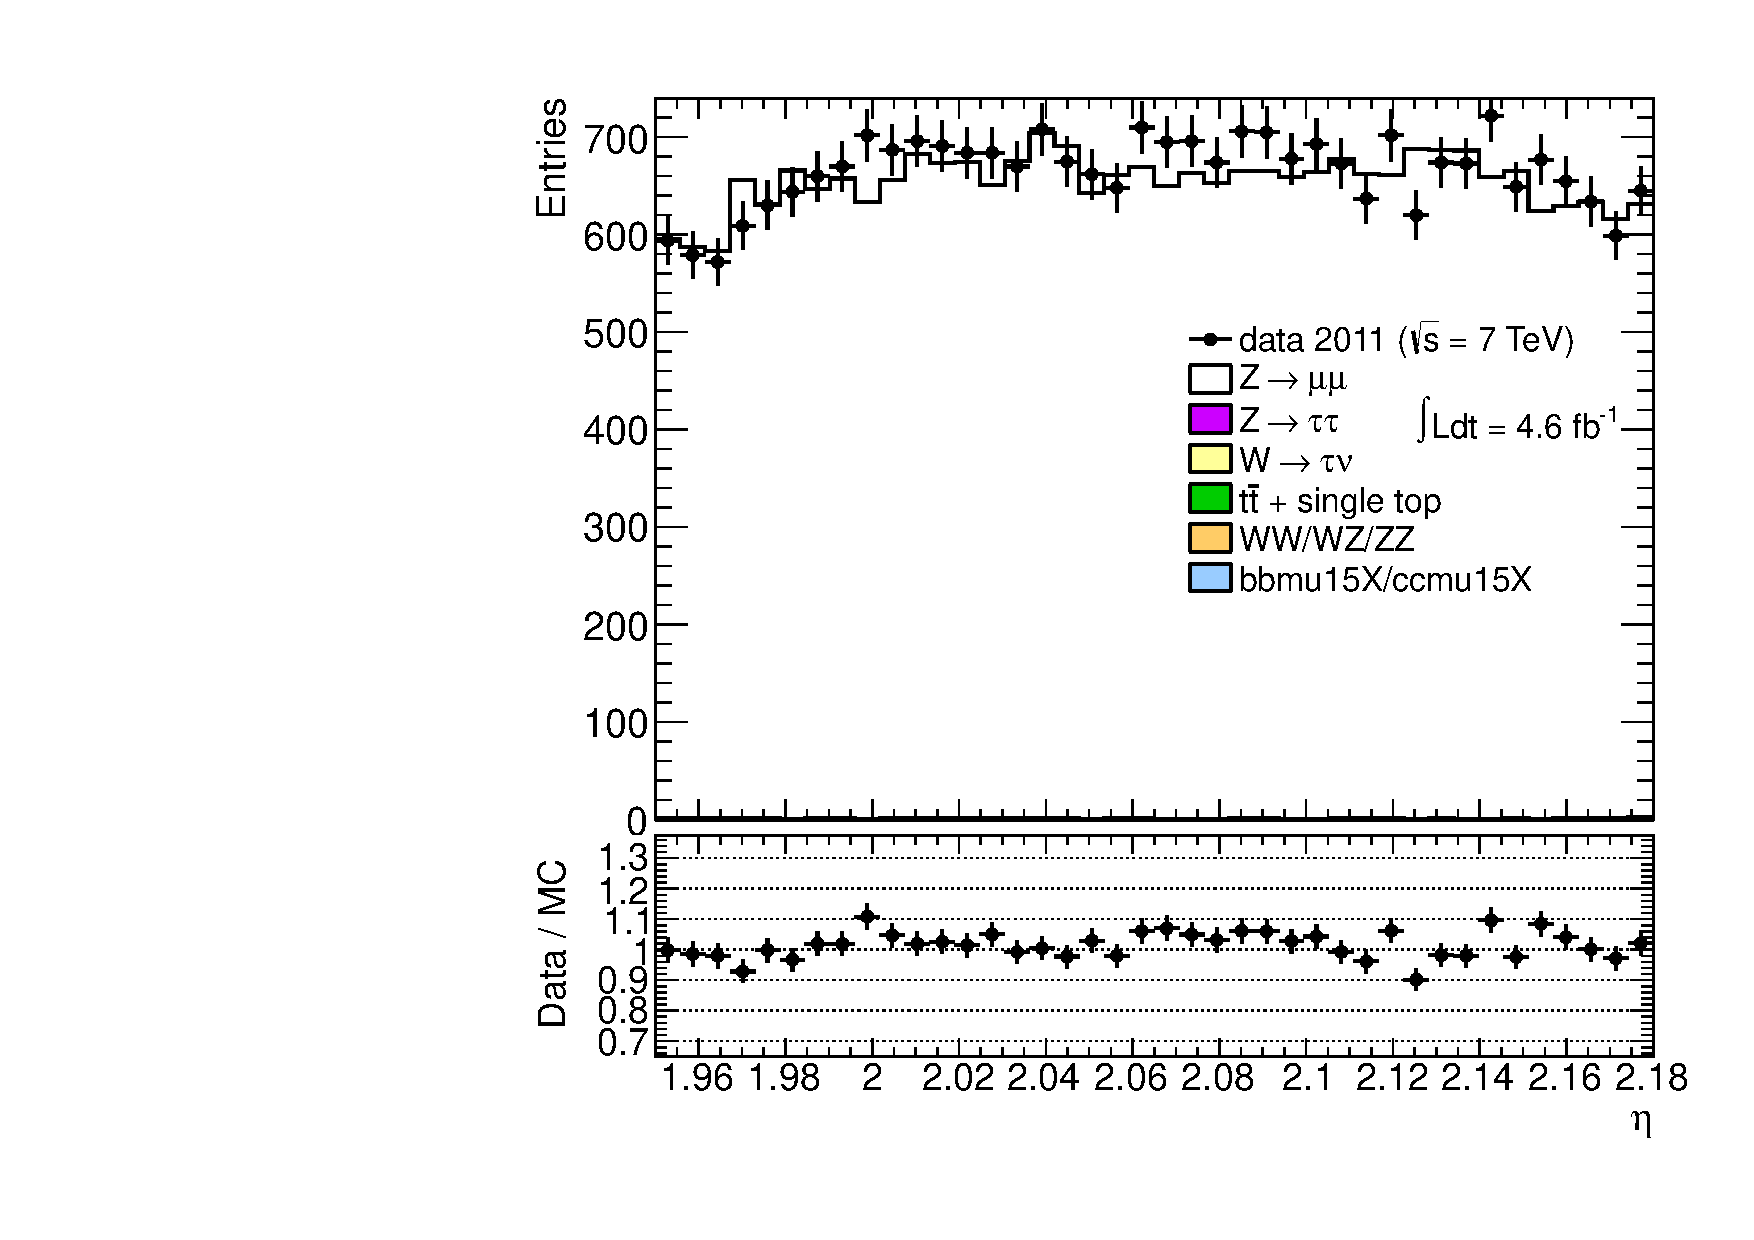
\includegraphics[width=0.66\textwidth]{dates/20130306/figures/both/ZlOendcap_10_A_stack_lN_eta_ALL.pdf} 
\cole
}

\slide{ $\mu^{-}$: ID-MS quality } {
What if we have very poorly reconstructed muons around the dip? \\
In that case, Z tag-and-probe and control plots would not see them \\
(because of the Z mass constraint) \\
Here, we apply a muon \red{ID-MS quality cut} (ID vs MS pT within 0.5\%)
}
\slide{ $\mu^{-}$: ID-MS quality } {
\colb[T]
\column{.5\textwidth}
C-side $\mu^{-}$ (top: W; bottom: Z)
\centering
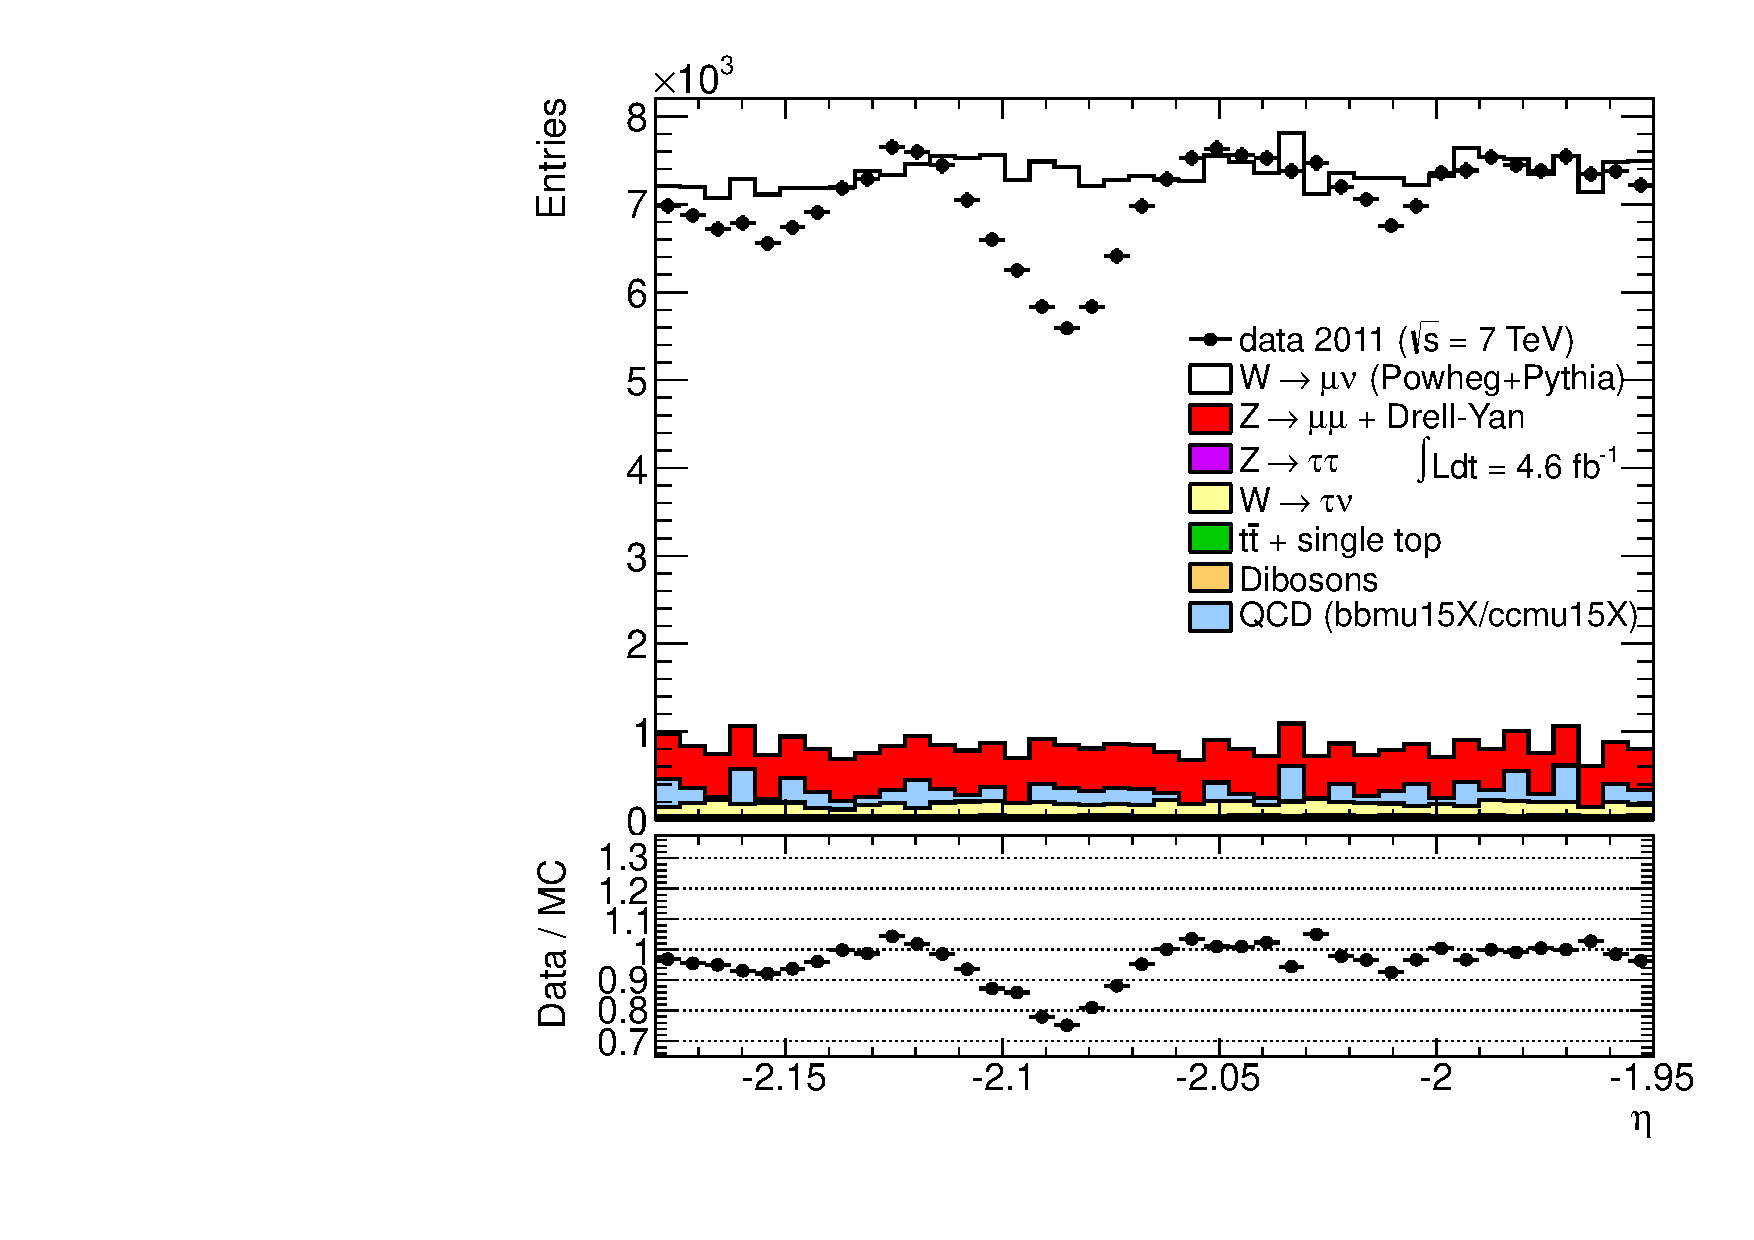
\includegraphics[width=0.66\textwidth]{dates/20130306/figures/both/Widms_10_C_stack_l_eta_NEG} \\
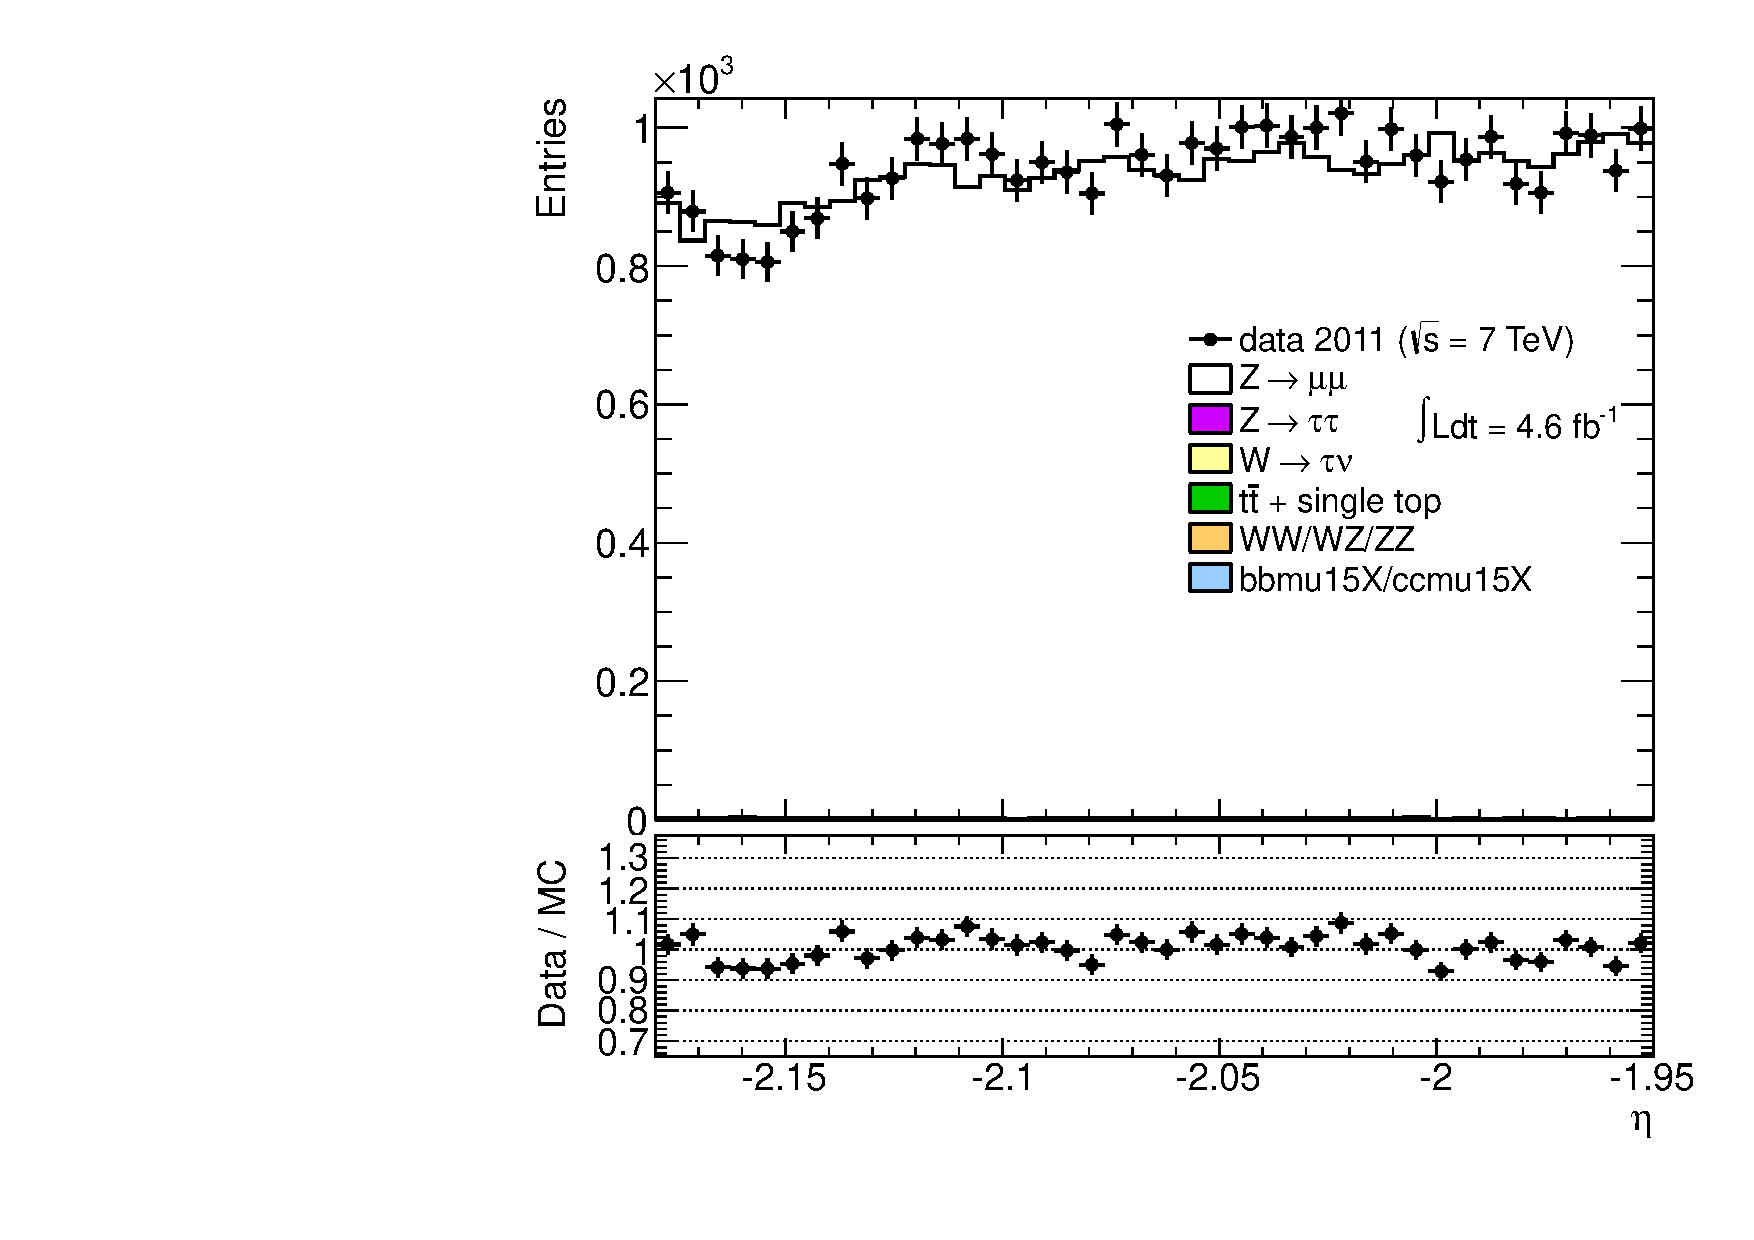
\includegraphics[width=0.66\textwidth]{dates/20130306/figures/both/Zidms_10_C_stack_lN_eta_ALL.pdf}
\column{.5\textwidth}
A-side $\mu^{-}$ (top: W; bottom: Z)
\centering
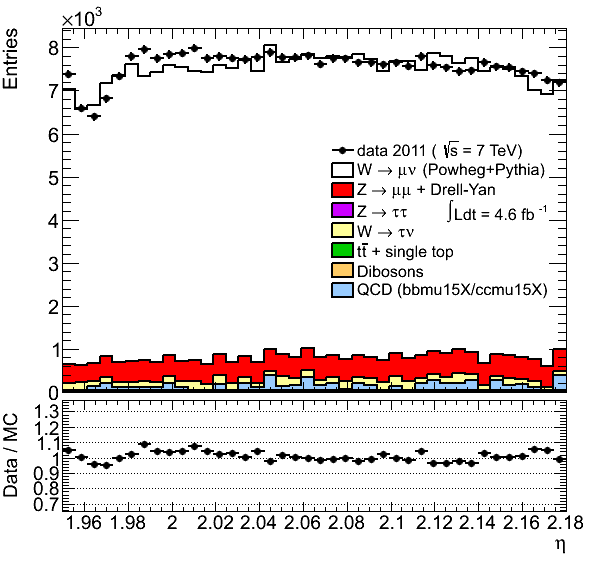
\includegraphics[width=0.66\textwidth]{dates/20130306/figures/both/Widms_10_A_stack_l_eta_NEG} \\
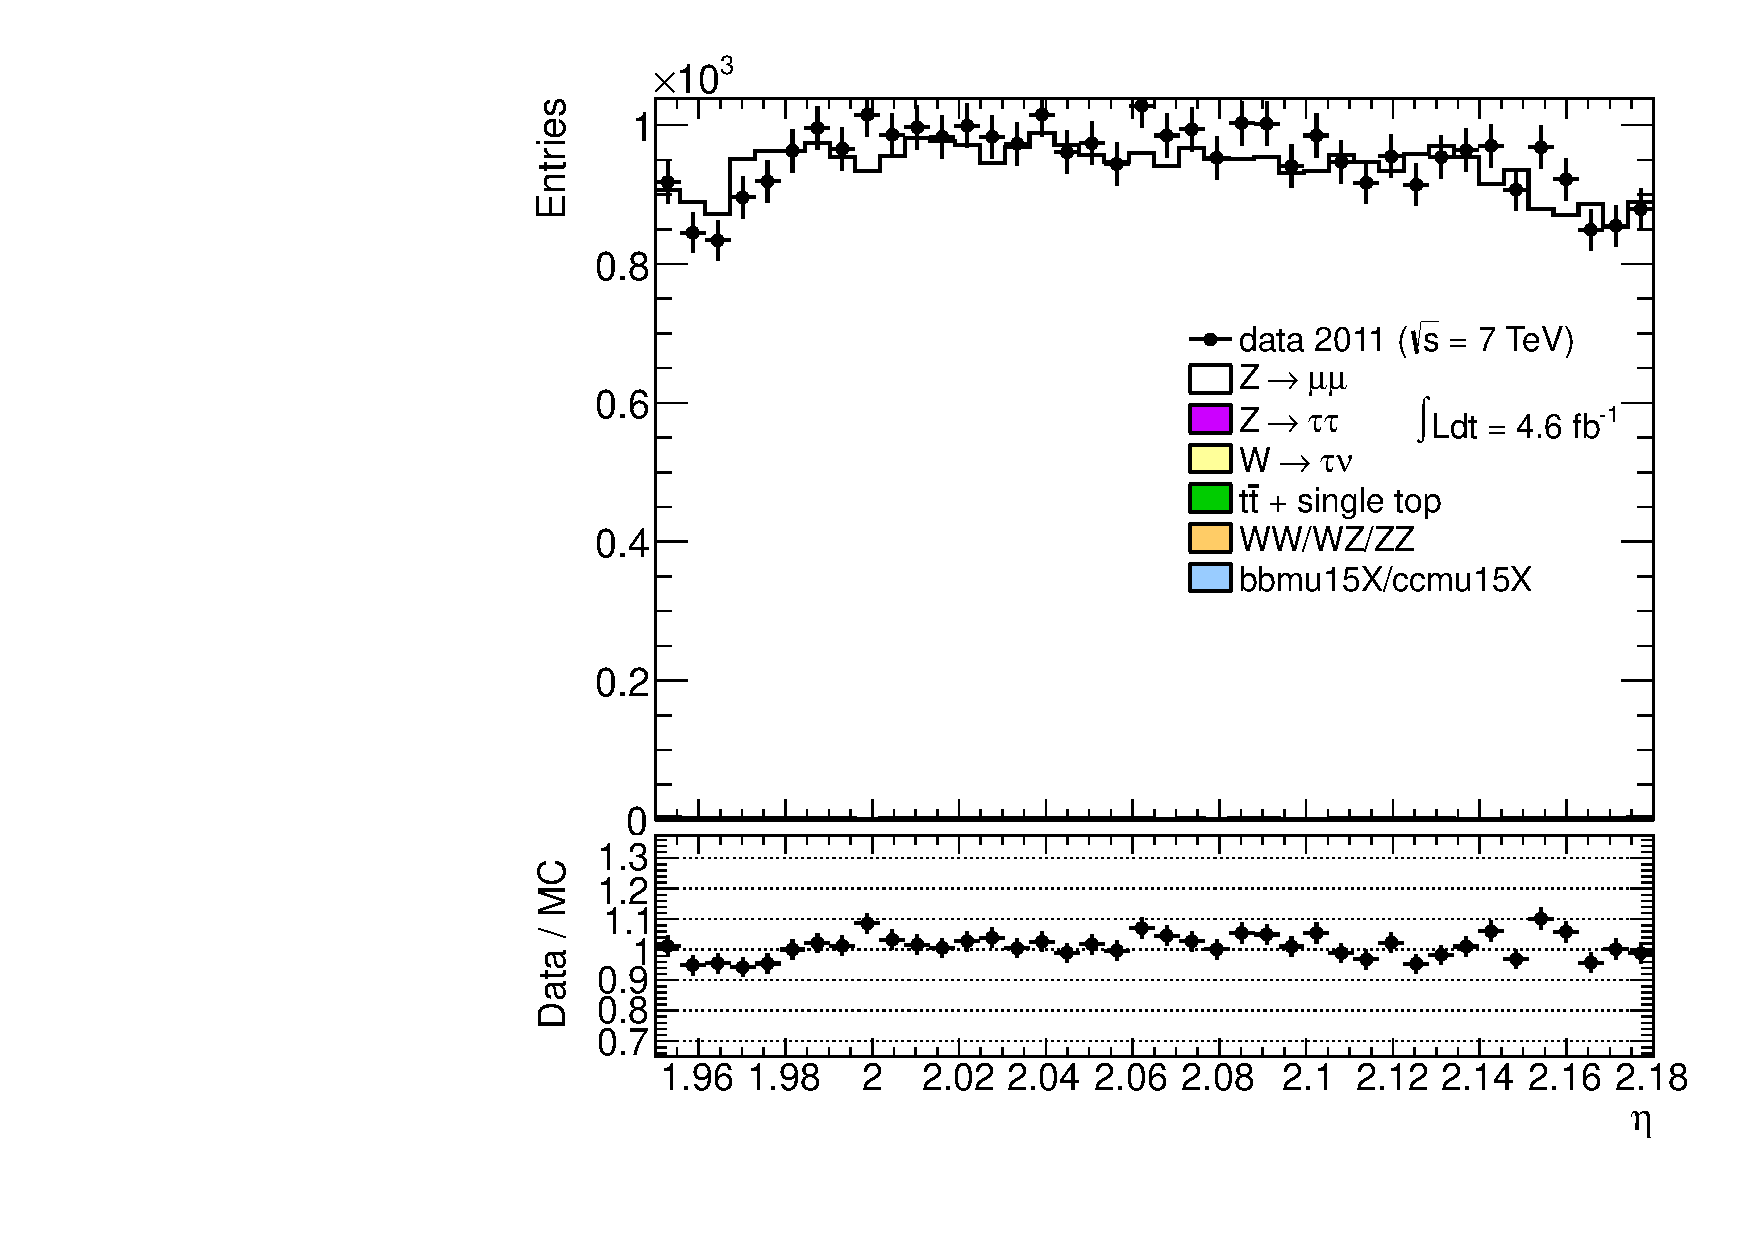
\includegraphics[width=0.66\textwidth]{dates/20130306/figures/both/Zidms_10_A_stack_lN_eta_ALL.pdf} 
\cole
}

\slide{ $\mu^{-}$: using ID pT } {
What if we have very poorly reconstructed muons around the dip? \\
In that case, Z tag-and-probe and control plots would not see them \\
(because of the Z mass constraint) \\
Here, we \red{use the muon pT measurement from ID only} (in W channel)
}
\slide{ $\mu^{-}$: using ID pT } {
\colb[T]
\column{.5\textwidth}
C-side $\mu^{-}$ (top: W; bottom: Z)
\centering
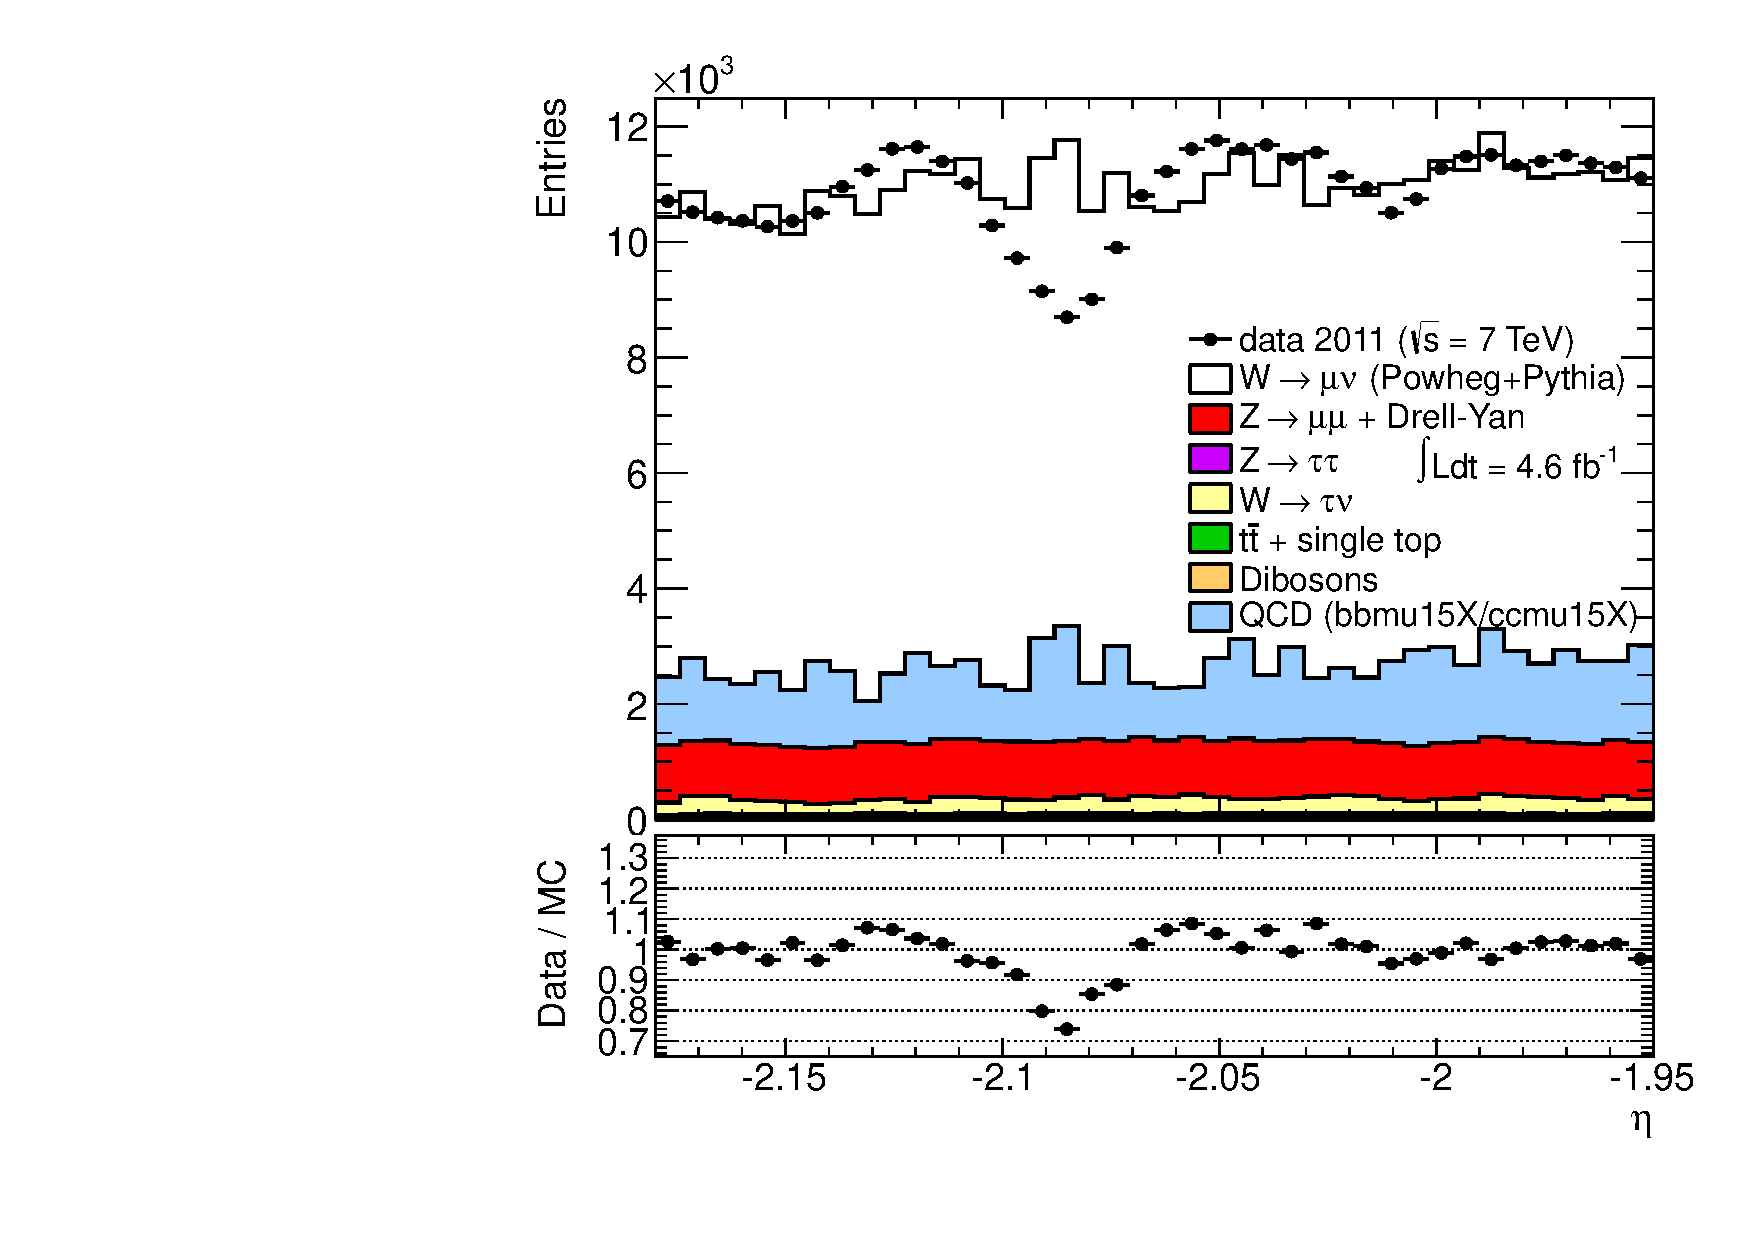
\includegraphics[width=0.66\textwidth]{dates/20130306/figures/both/Wnometmtid_10_C_stack_l_eta_NEG} \\
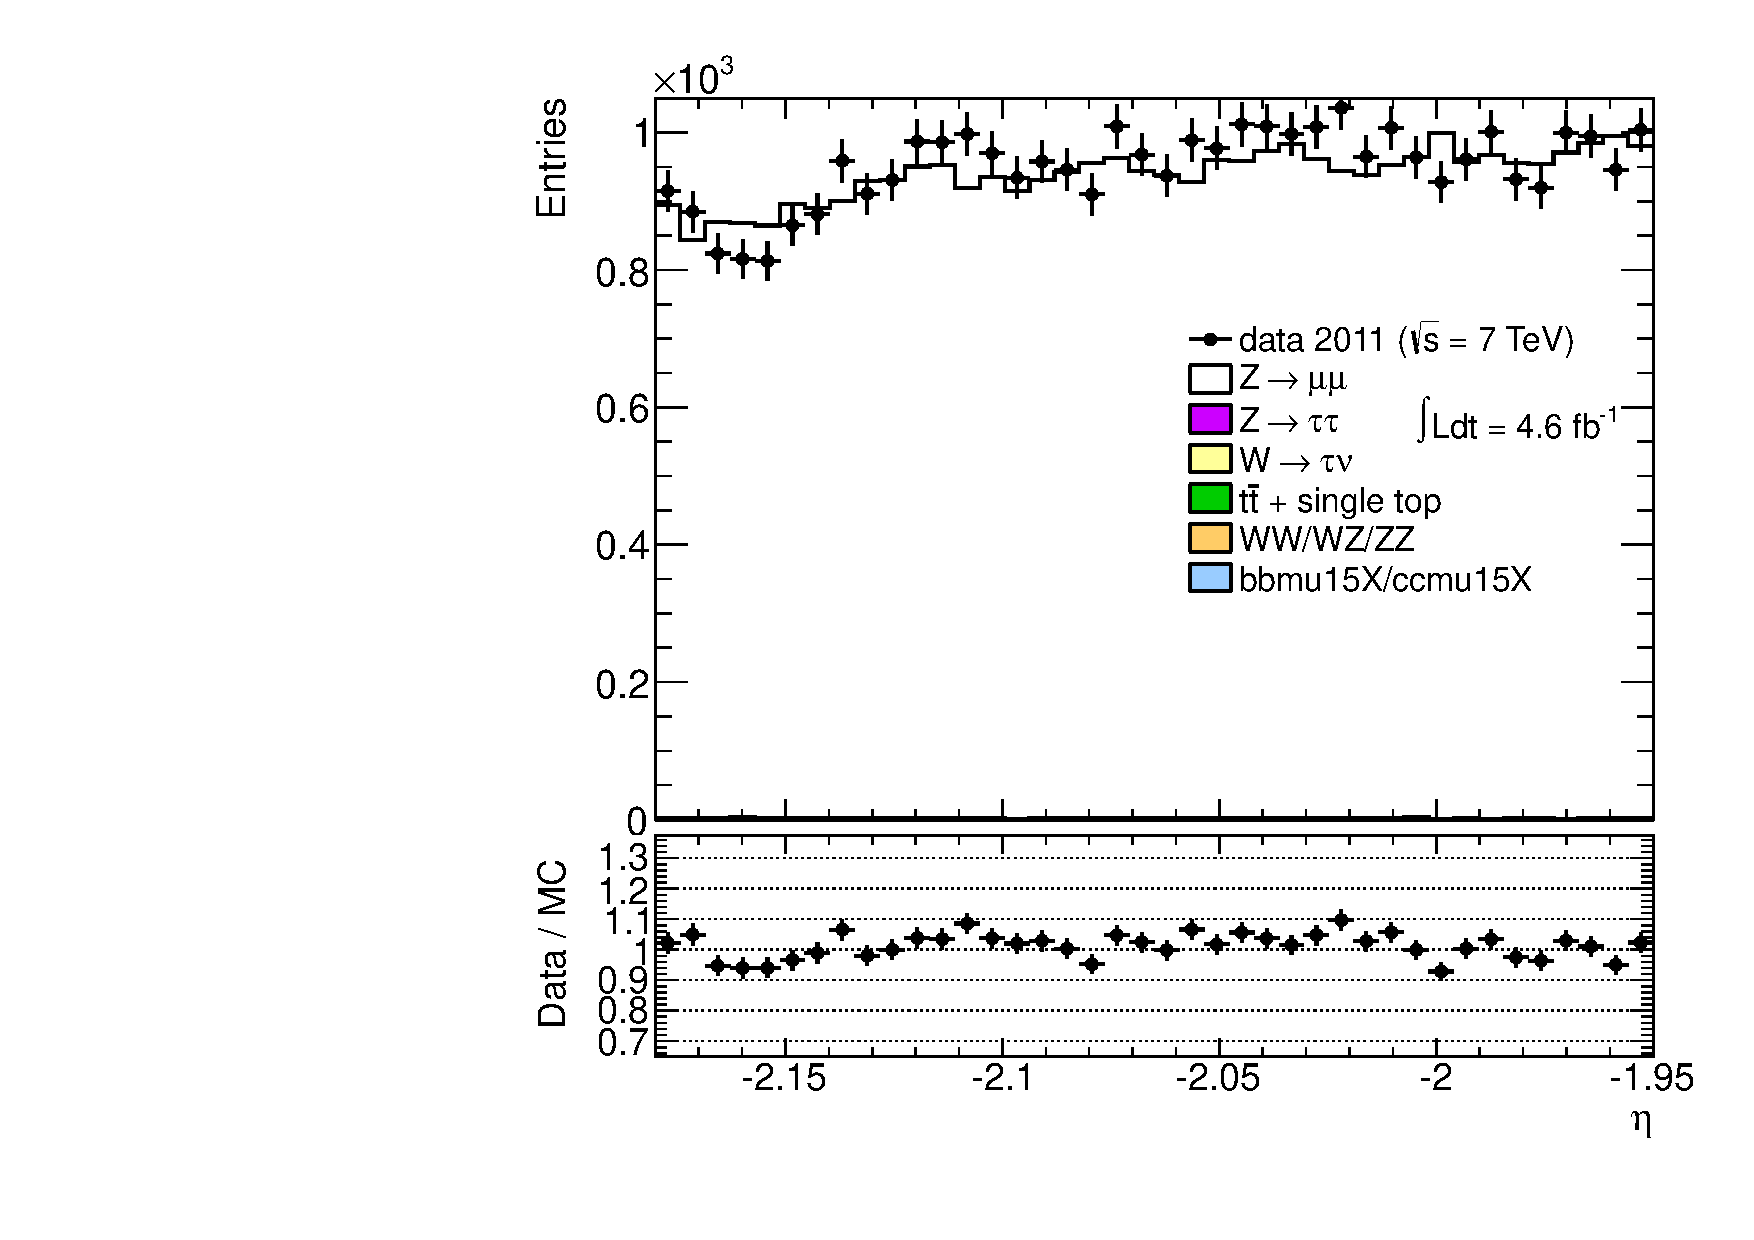
\includegraphics[width=0.66\textwidth]{dates/20130306/figures/both/Z_10_C_stack_lN_eta_ALL.pdf}
\column{.5\textwidth}
A-side $\mu^{-}$ (top: W; bottom: Z)
\centering
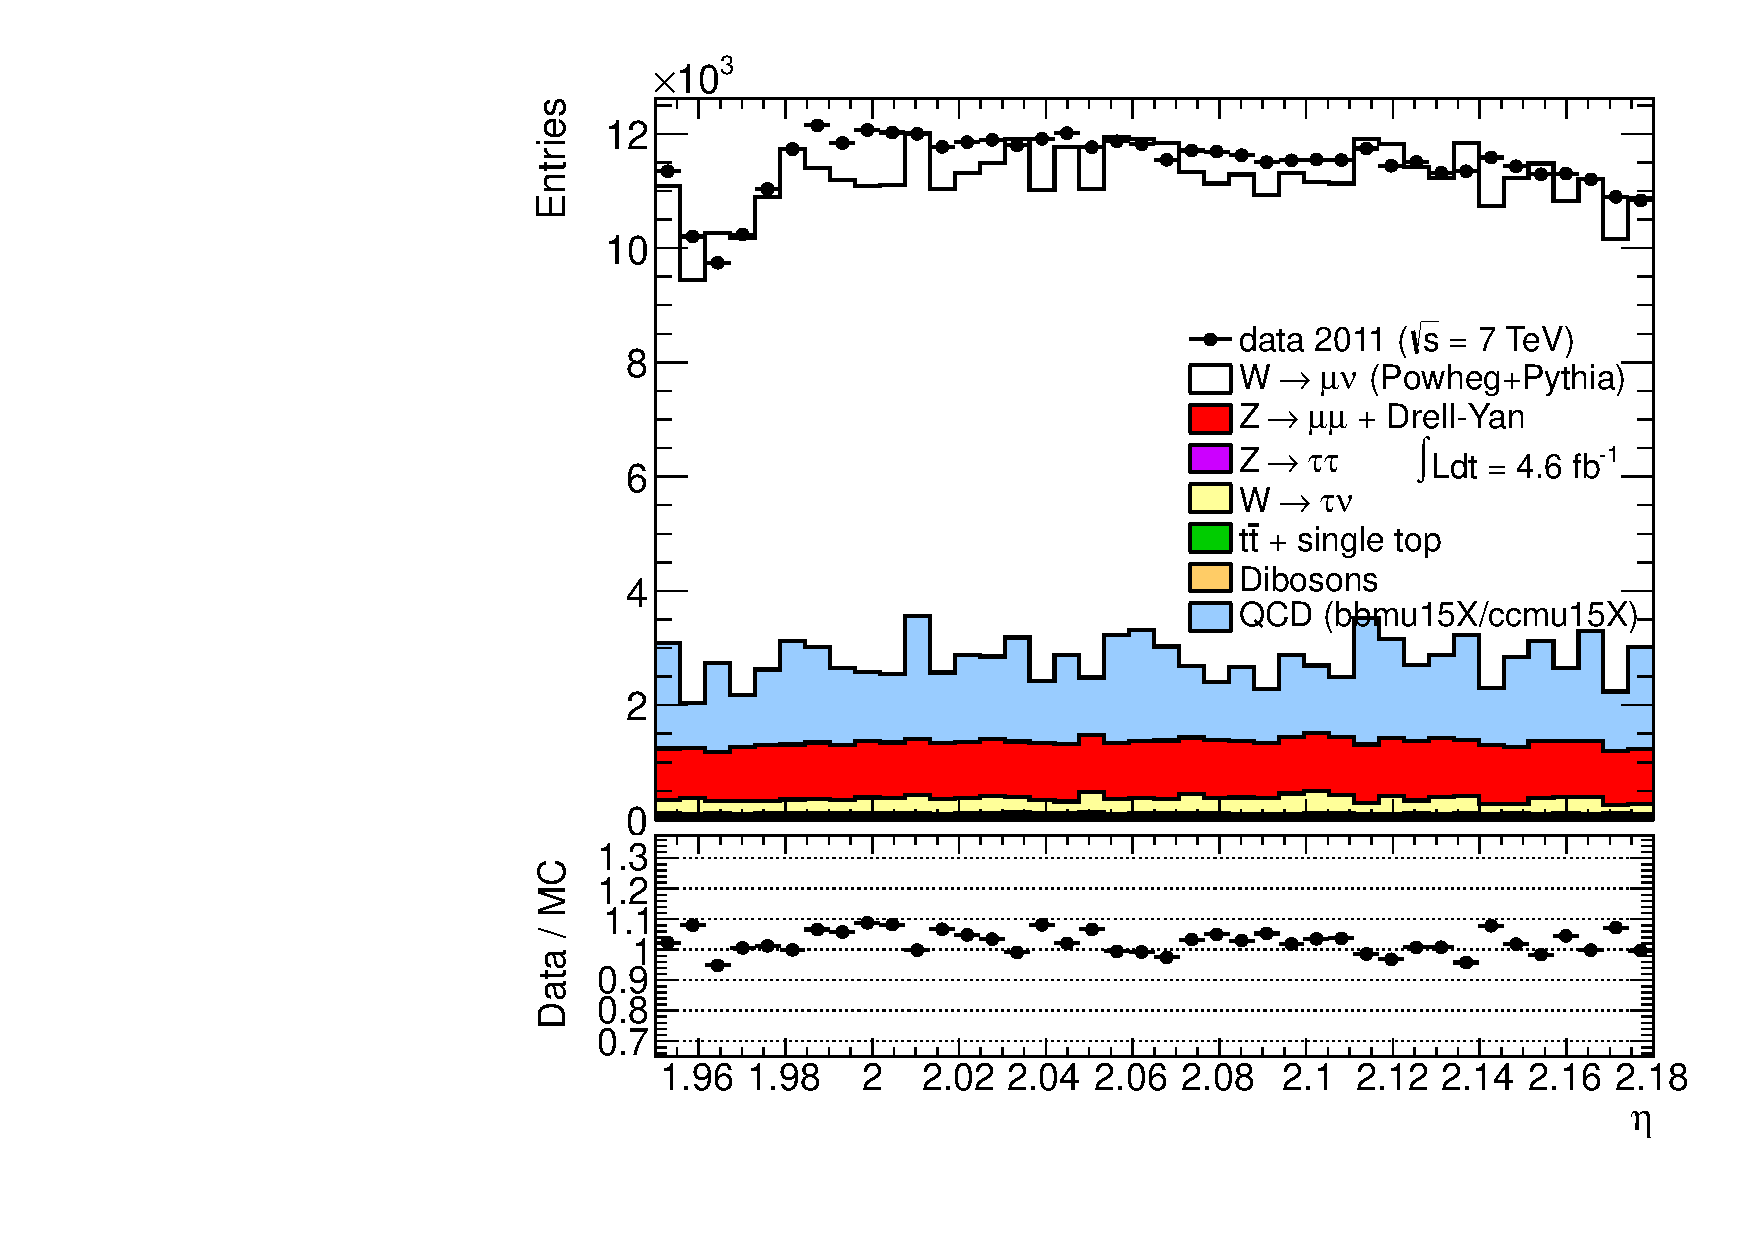
\includegraphics[width=0.66\textwidth]{dates/20130306/figures/both/Wnometmtid_10_A_stack_l_eta_NEG} \\
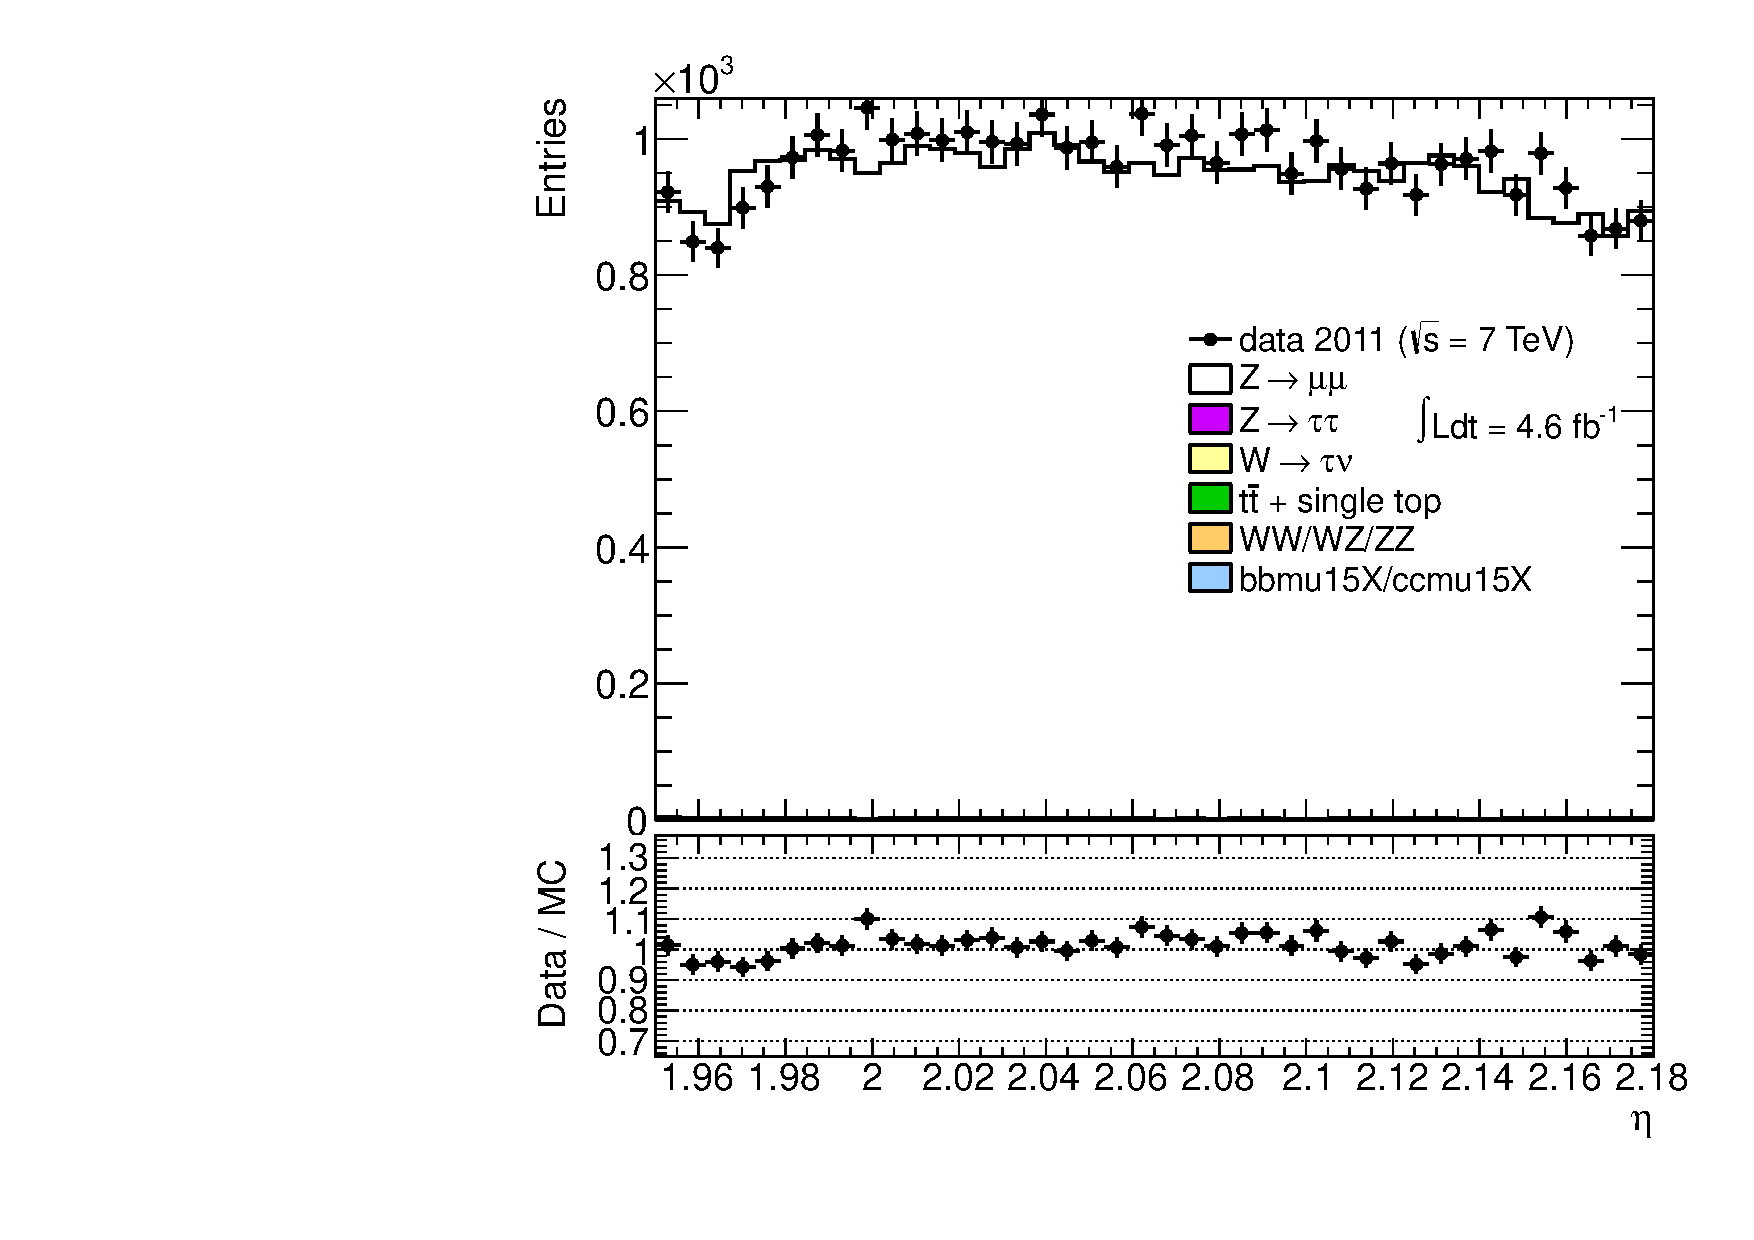
\includegraphics[width=0.66\textwidth]{dates/20130306/figures/both/Z_10_A_stack_lN_eta_ALL.pdf} 
\cole
}

\slide{ $\mu^{-}$: Z without inv. mass } {
What if we have very poorly reconstructed muons around the dip? \\
In that case, Z tag-and-probe and control plots would not see them \\
(because of the Z mass constraint) \\
Here, we \red{completely drop the Z mass constraint}
}
\slide{ $\mu^{-}$: Z without inv. mass } {
\colb[T]
\column{.5\textwidth}
C-side $\mu^{-}$ (top: W; bottom: Z)
\centering
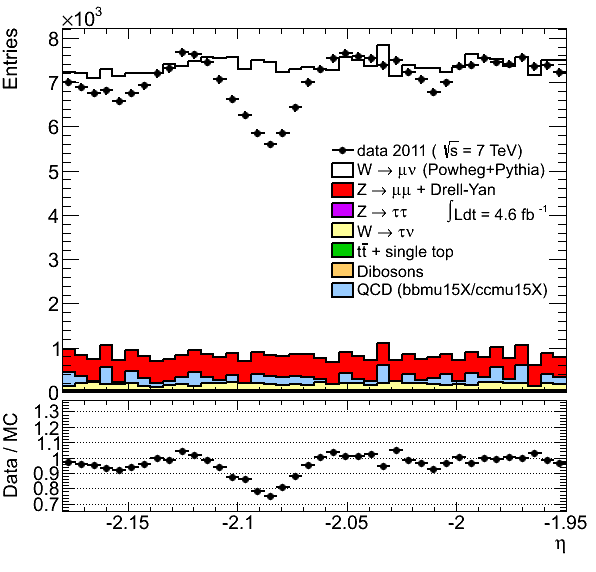
\includegraphics[width=0.66\textwidth]{dates/20130306/figures/both/W_10_C_stack_l_eta_NEG} \\
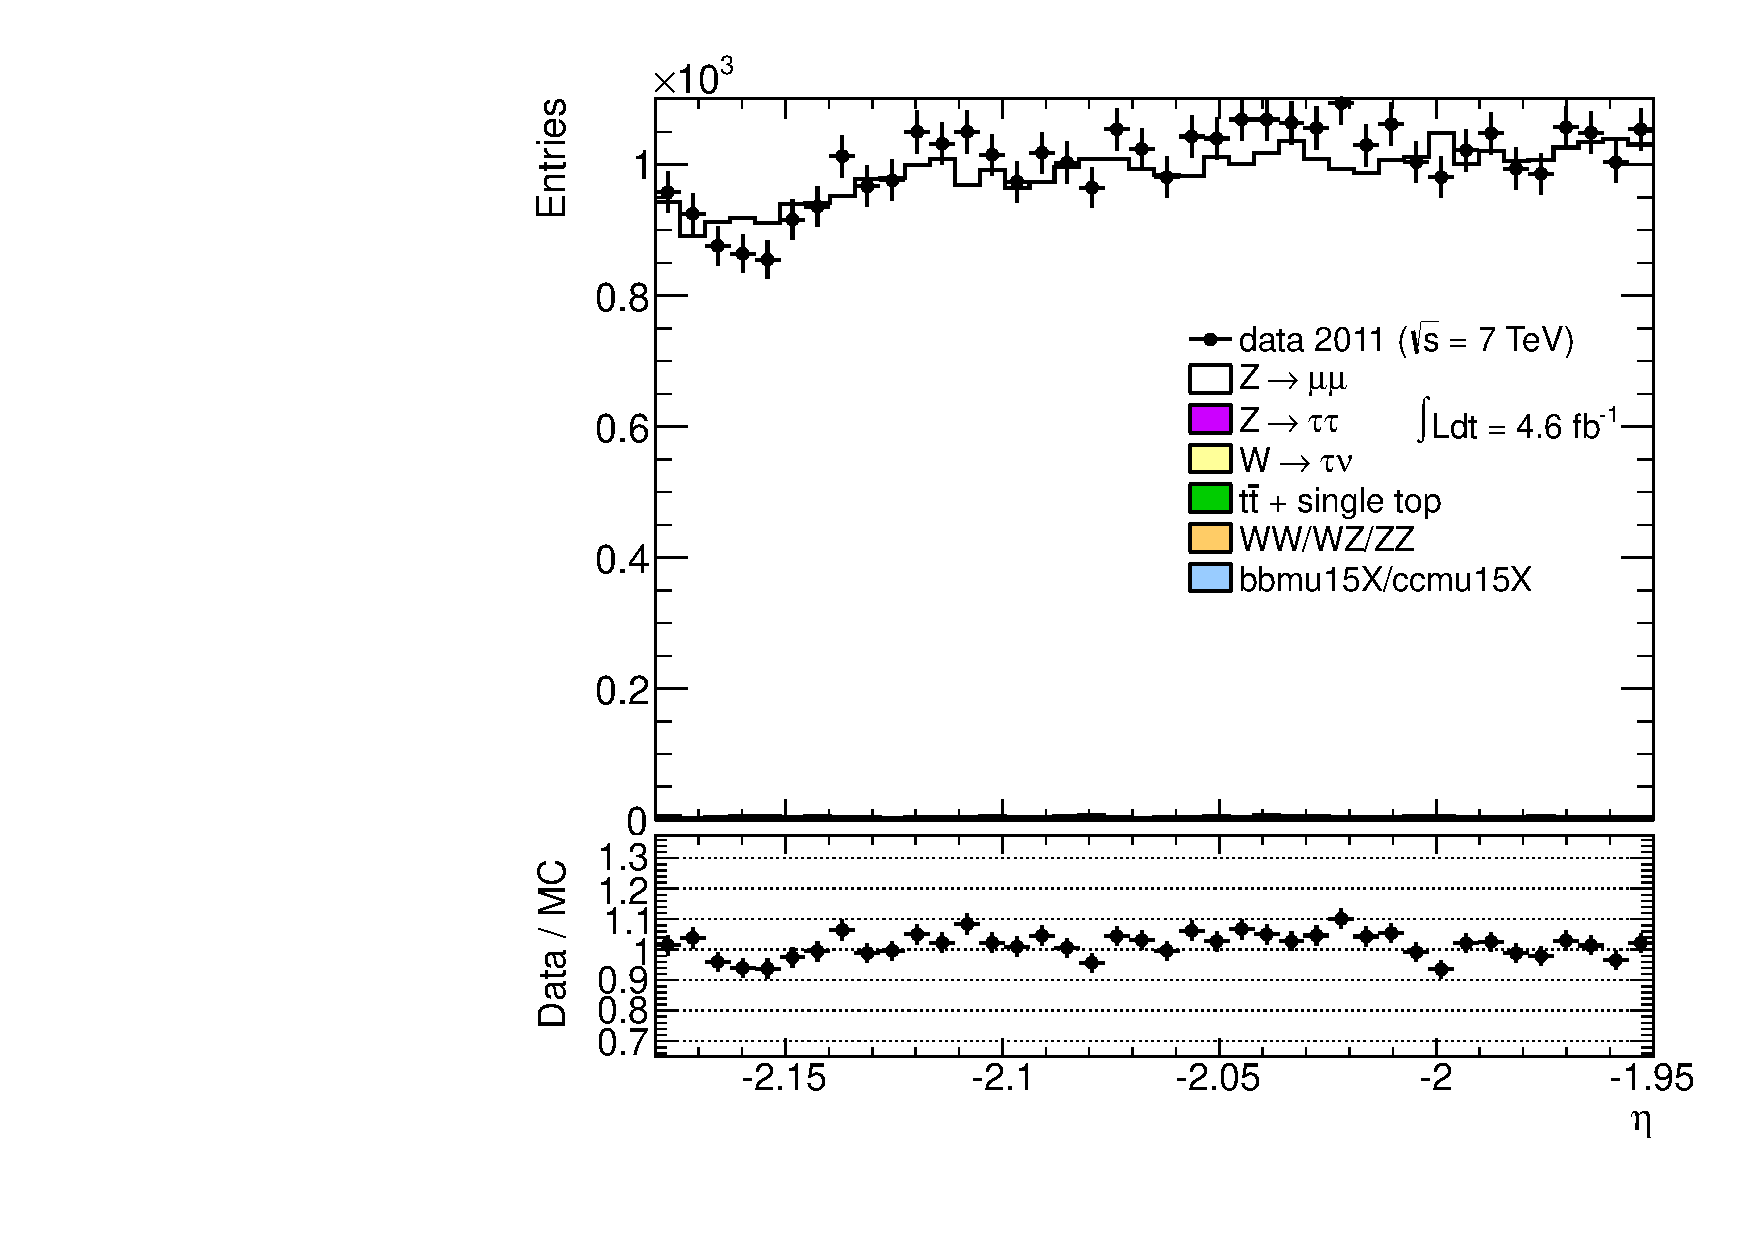
\includegraphics[width=0.66\textwidth]{dates/20130306/figures/both/Znowind_10_C_stack_lN_eta_ALL.pdf}
\column{.5\textwidth}
A-side $\mu^{-}$ (top: W; bottom: Z)
\centering
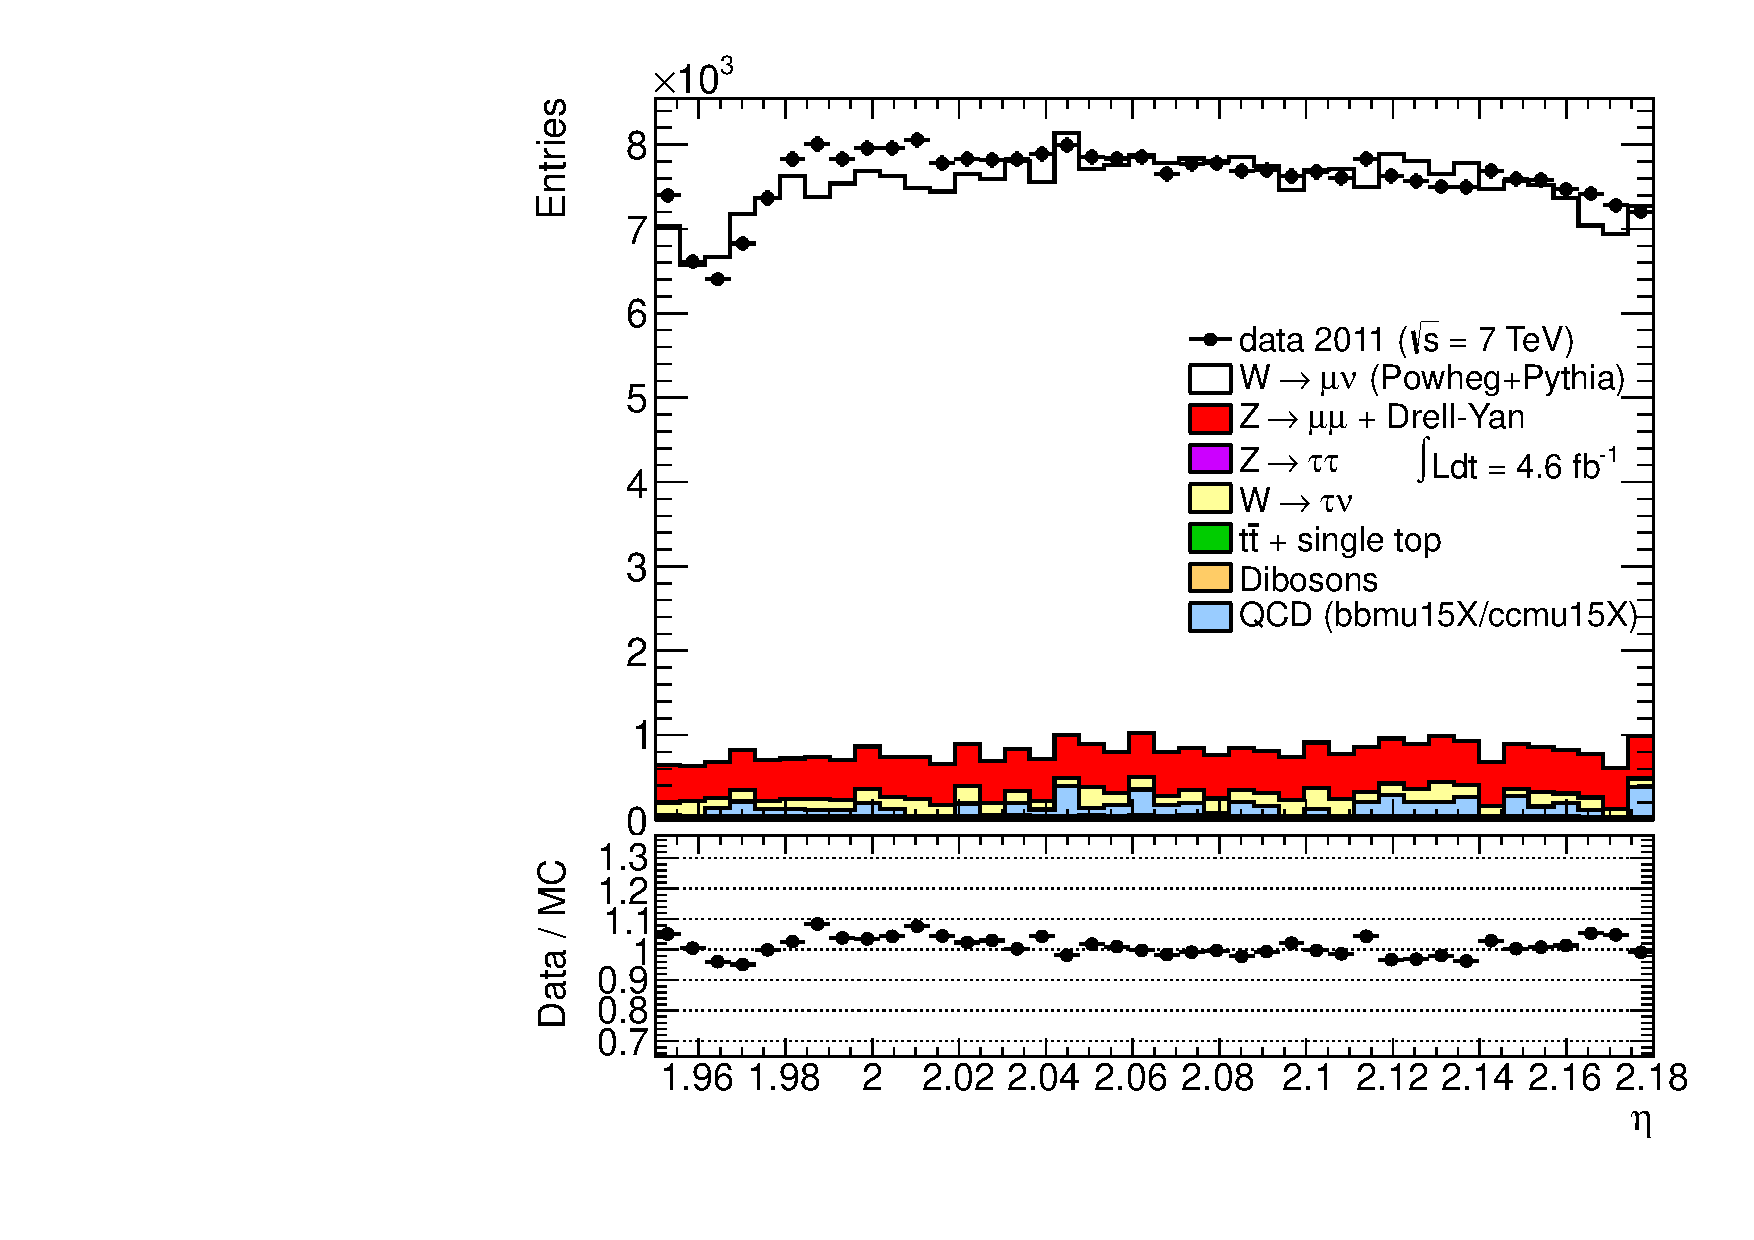
\includegraphics[width=0.66\textwidth]{dates/20130306/figures/both/W_10_A_stack_l_eta_NEG} \\
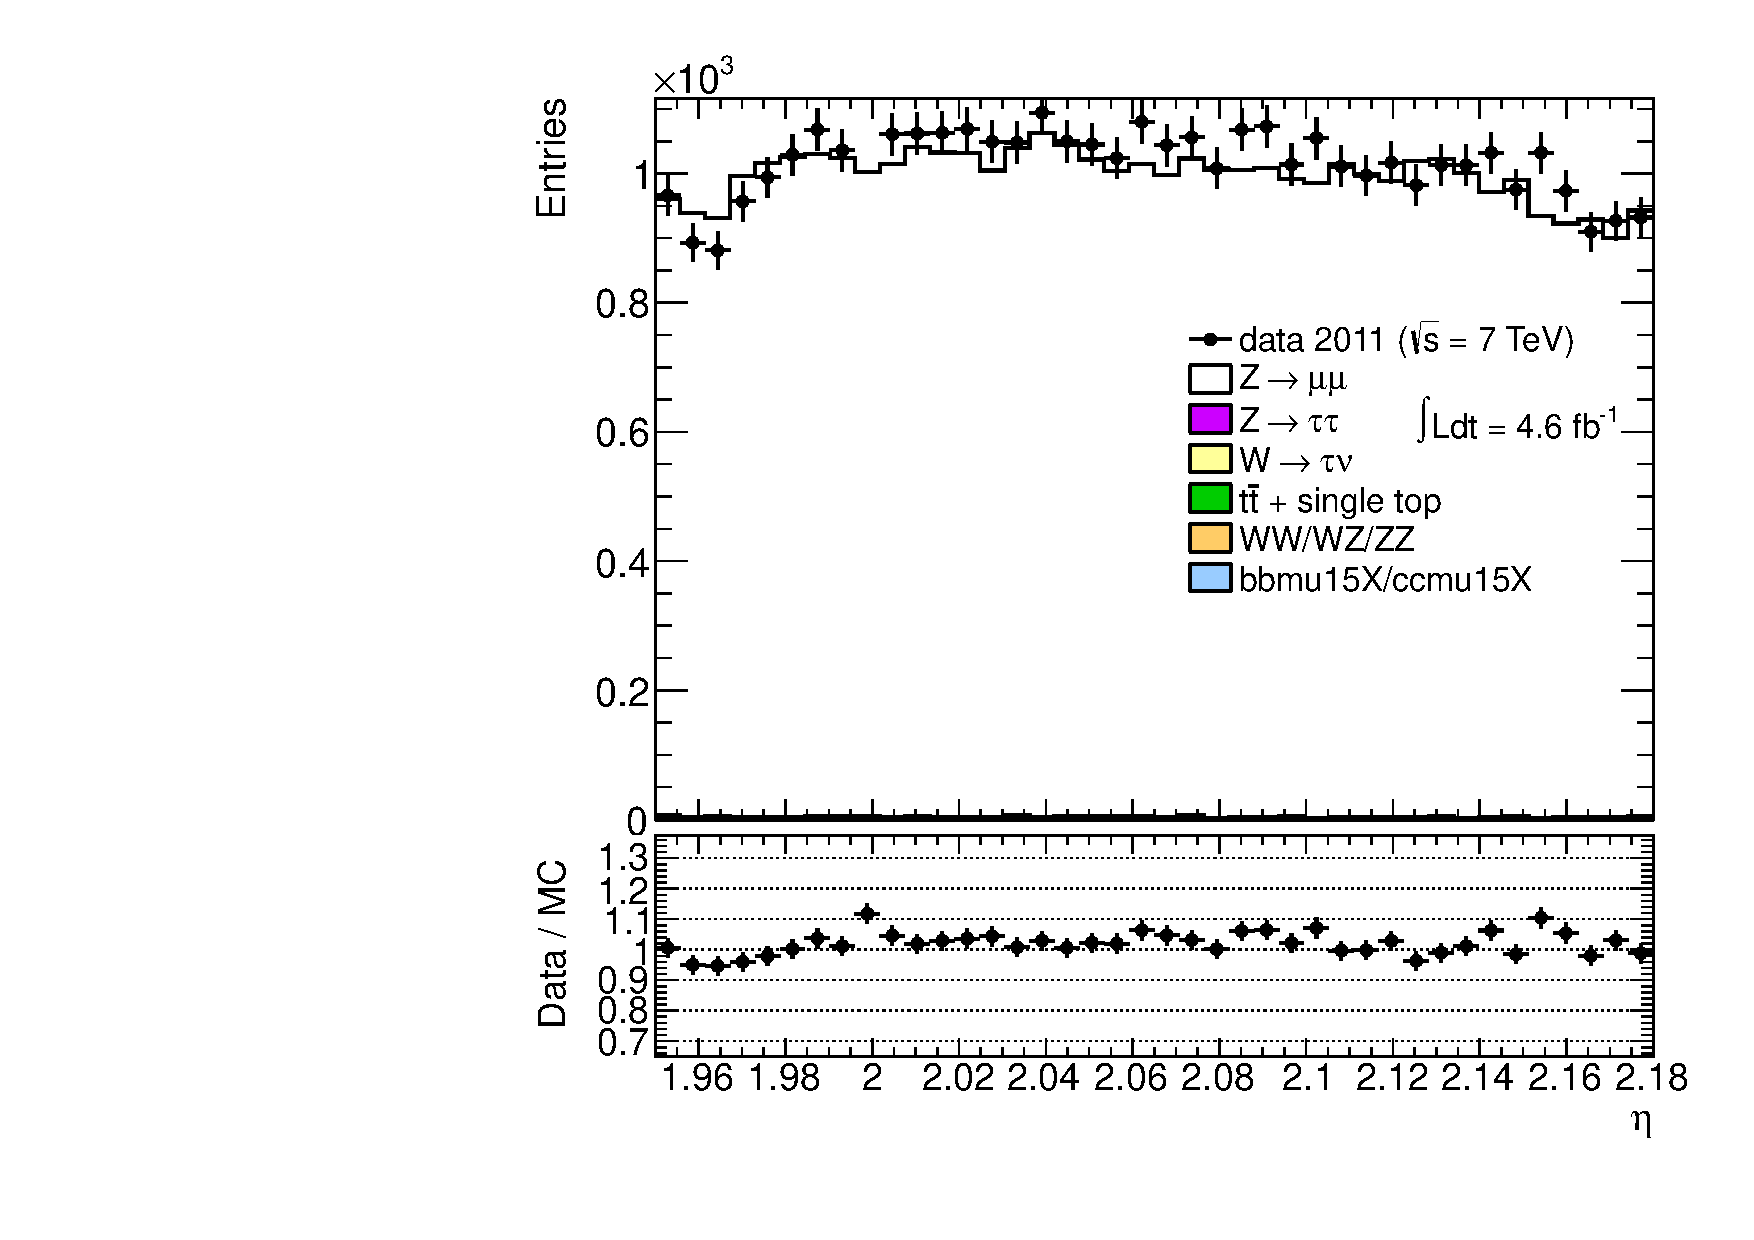
\includegraphics[width=0.66\textwidth]{dates/20130306/figures/both/Znowind_10_A_stack_lN_eta_ALL.pdf} 
\cole
}


\slide{ $\mu^{-}$: W with extra muons } {
What in the world could cause the dip in W selection? \\
Let's try dropping various cuts in the W selection. \\
Drop \red{nmuons==1 cut} (i.e. allow additional muons in an event).
}
\slide{ $\mu^{-}$: W with extra muons } {
\colb[T]
\column{.5\textwidth}
C-side $\mu^{-}$ (top: W; bottom: Z)
\centering
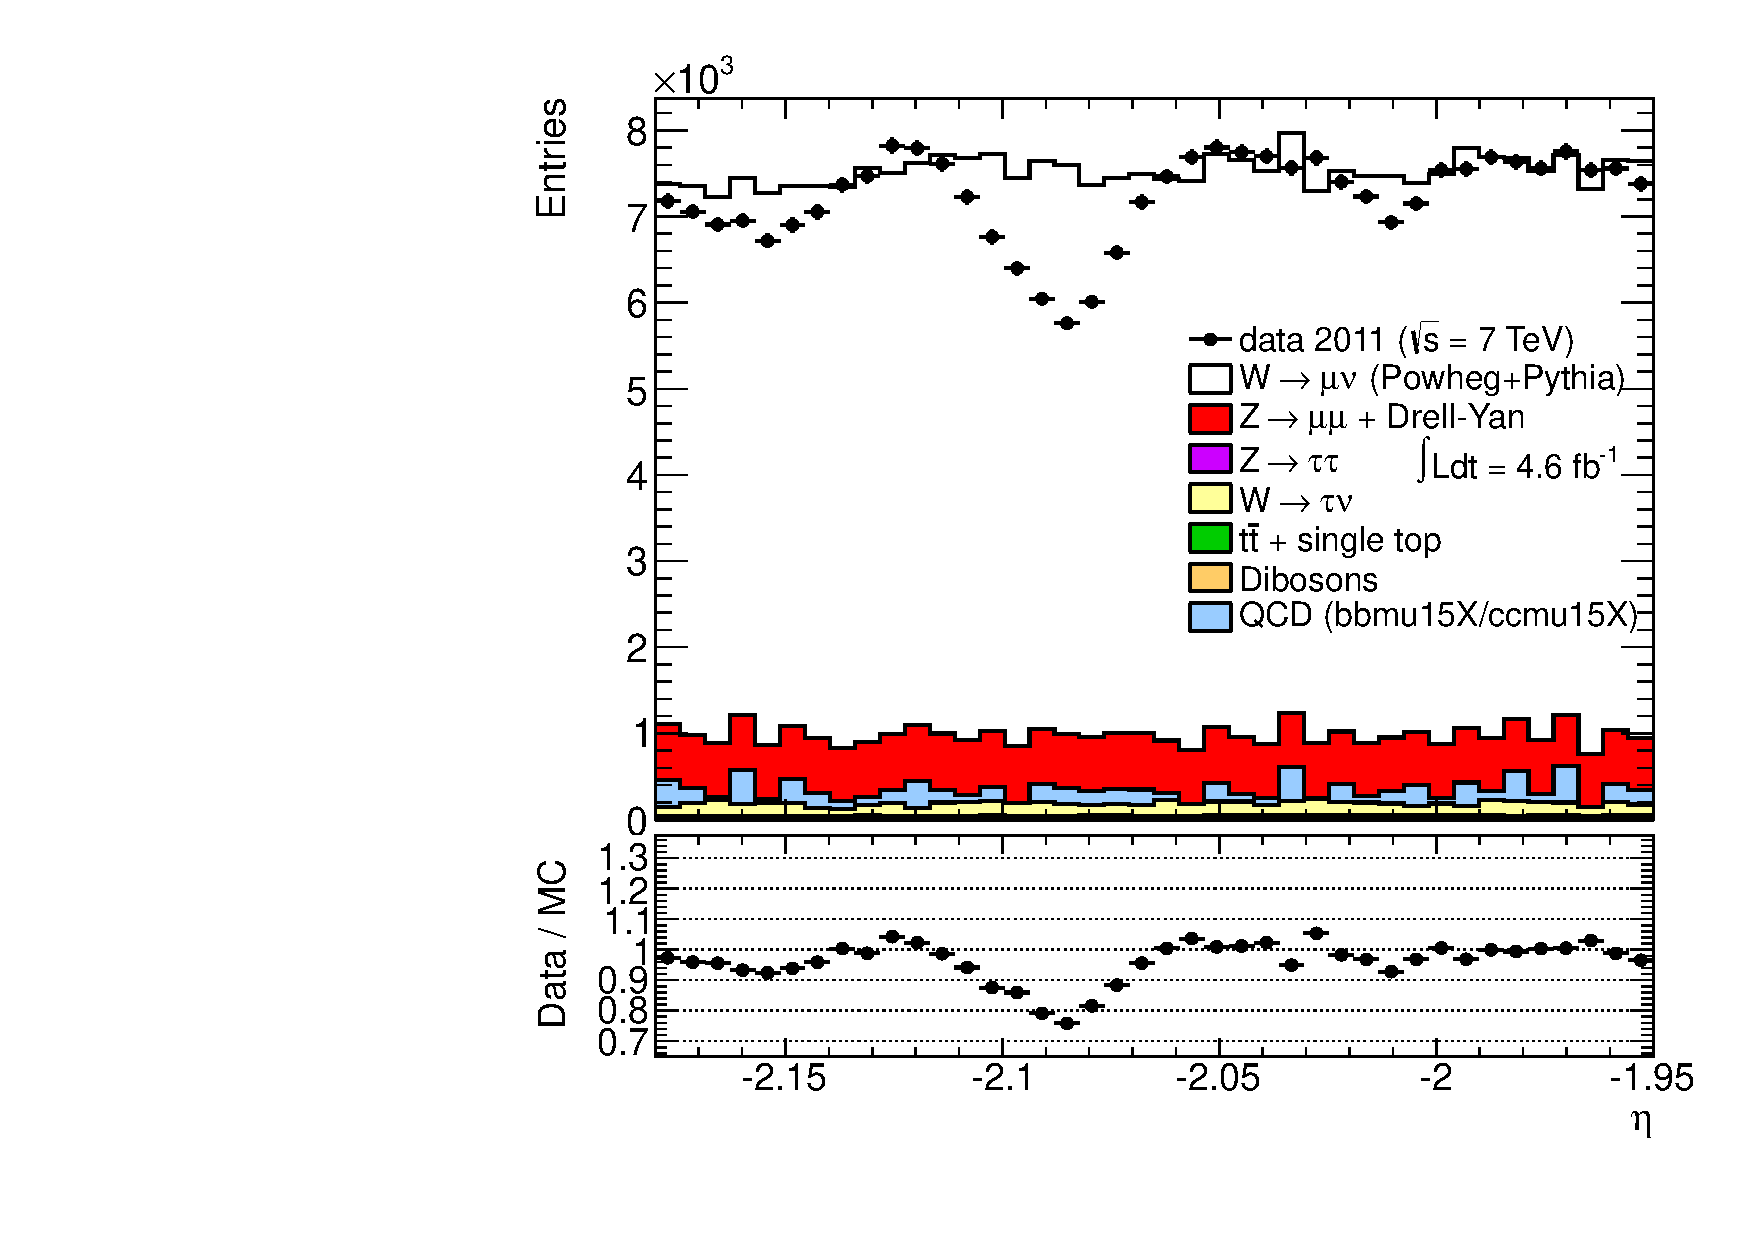
\includegraphics[width=0.66\textwidth]{dates/20130306/figures/both/Wnonmu_10_C_stack_l_eta_NEG} \\
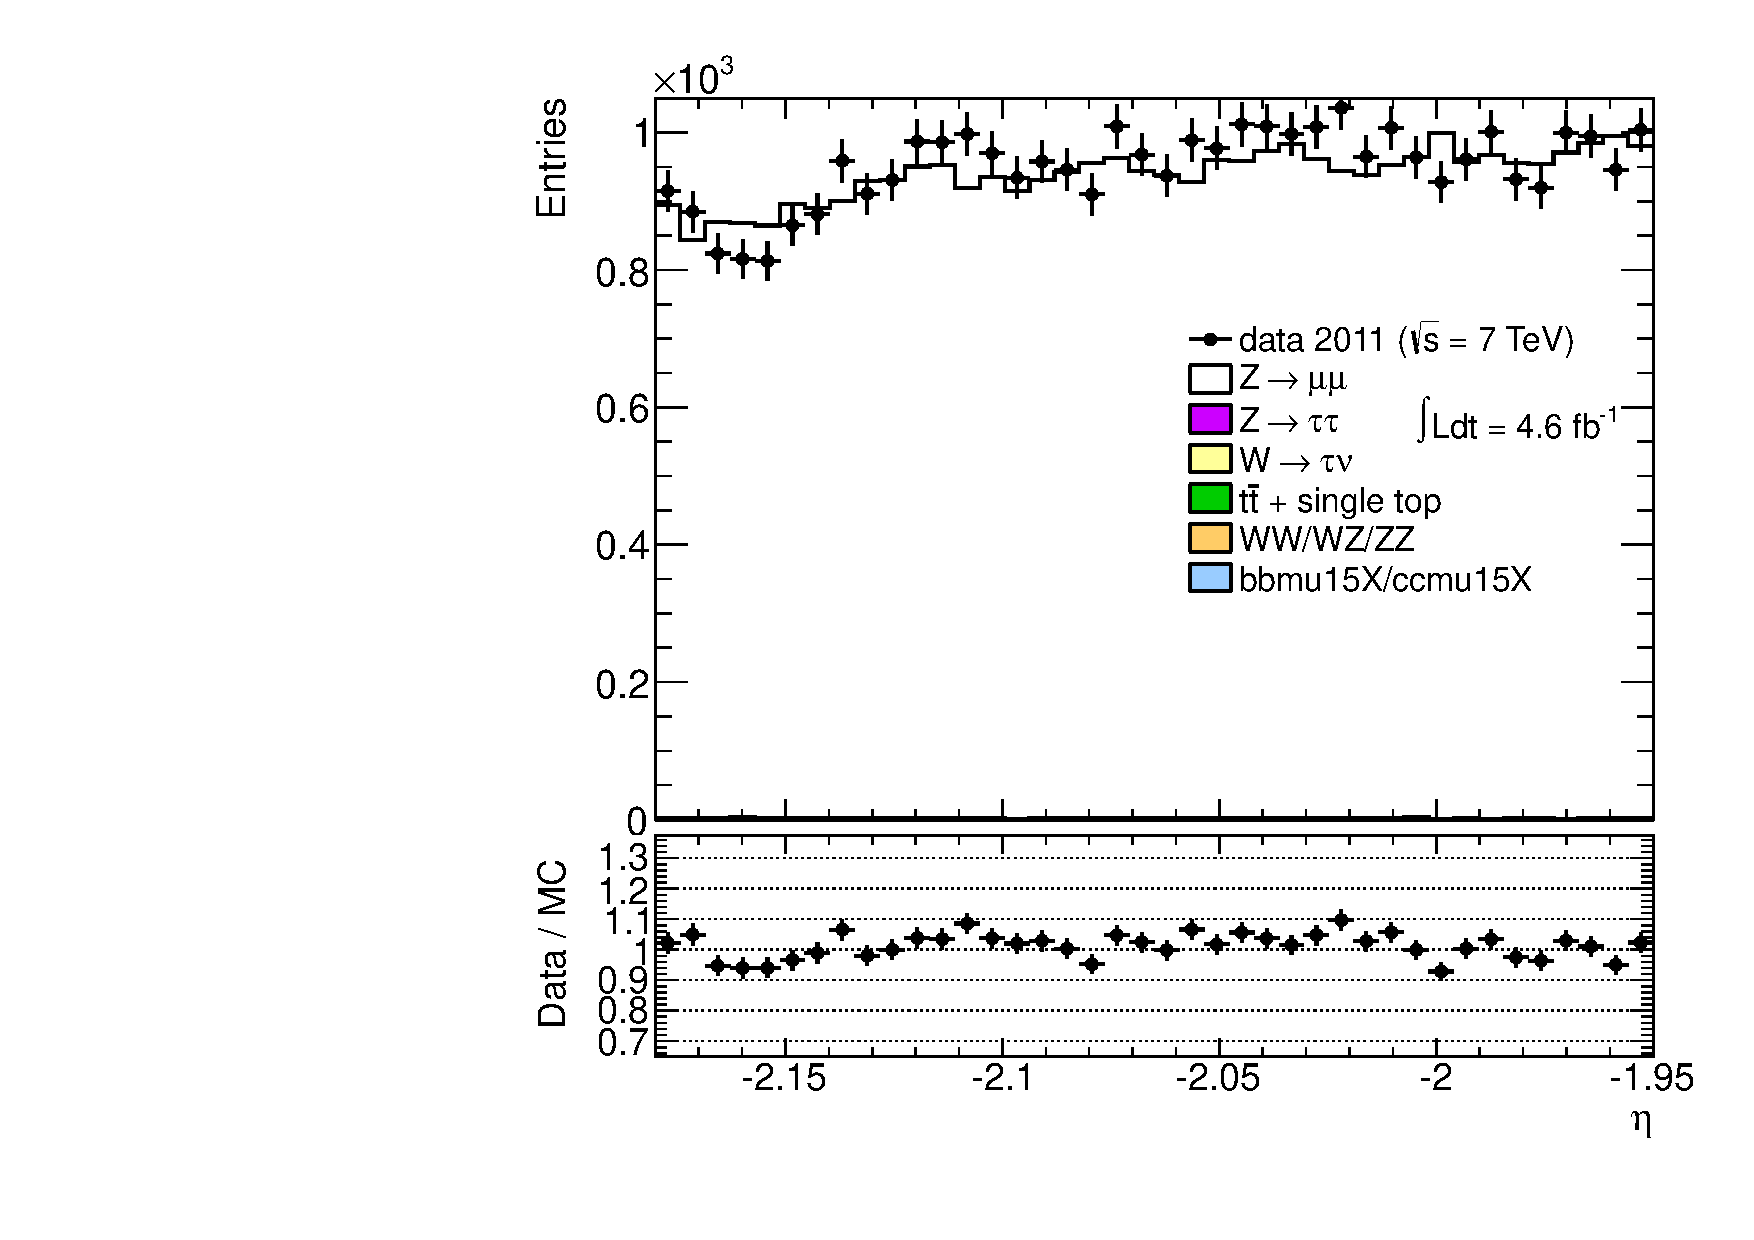
\includegraphics[width=0.66\textwidth]{dates/20130306/figures/both/Z_10_C_stack_lN_eta_ALL.pdf}
\column{.5\textwidth}
A-side $\mu^{-}$ (top: W; bottom: Z)
\centering
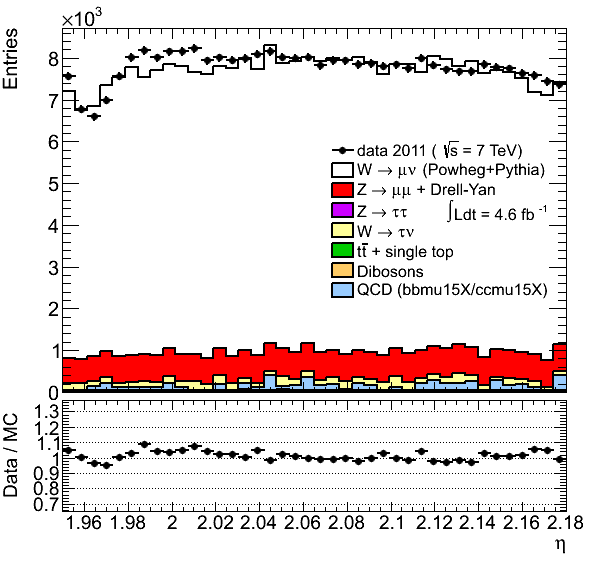
\includegraphics[width=0.66\textwidth]{dates/20130306/figures/both/Wnonmu_10_A_stack_l_eta_NEG} \\
\includegraphics[width=0.66\textwidth]{dates/20130306/figures/both/Z_10_A_stack_lN_eta_ALL.pdf} 
\cole
}

\slide{ $\mu^{-}$: W with extra muons } {
What in the world could cause the dip in W selection? \\
Let's try dropping various cuts in the W selection. \\
Drop \red{all cuts}, except: one 15-GeV muon (MCP-quality)
}
\slide{ $\mu^{-}$: W with extra muons } {
\colb[T]
\column{.5\textwidth}
C-side $\mu^{-}$ (top: W; bottom: Z)
\centering
\includegraphics[width=0.66\textwidth]{dates/20130306/figures/both/Wnocuts_10_C_stack_l_eta_NEG} \\
\includegraphics[width=0.66\textwidth]{dates/20130306/figures/both/Z_10_C_stack_lN_eta_ALL.pdf}
\column{.5\textwidth}
A-side $\mu^{-}$ (top: W; bottom: Z)
\centering
\includegraphics[width=0.66\textwidth]{dates/20130306/figures/both/Wnocuts_10_A_stack_l_eta_NEG} \\
\includegraphics[width=0.66\textwidth]{dates/20130306/figures/both/Z_10_A_stack_lN_eta_ALL.pdf} 
\cole
}

\slide{ $\mu^{-}$: sanity check of W ntuple } {
OK, the dip is still seen. Is there a bug in my W ntuple? \\
Let's use my W ntuple, but force nmuons==2. This should select mostly Z events. \\
(in this test, no Z mass or opposite charges constraint is applied)
}
\slide{ $\mu^{-}$: sanity check of W ntuple } {
\colb[T]
\column{.5\textwidth}
C-side $\mu^{-}$ (top: W; bottom: Z)
\centering
\includegraphics[width=0.66\textwidth]{dates/20130306/figures/both/Wzlike_10_C_stack_l_eta_NEG} \\
\includegraphics[width=0.66\textwidth]{dates/20130306/figures/both/Z_10_C_stack_lN_eta_ALL.pdf}
\column{.5\textwidth}
A-side $\mu^{-}$ (top: W; bottom: Z)
\centering
\includegraphics[width=0.66\textwidth]{dates/20130306/figures/both/Wzlike_10_A_stack_l_eta_NEG} \\
\includegraphics[width=0.66\textwidth]{dates/20130306/figures/both/Z_10_A_stack_lN_eta_ALL.pdf} 
\cole
}

\slide{ $\mu^{-}$: fate of the dip in W vs $\phi$ } {
Let's see what happens with the dip in W in four $\phi$ quadrants.
}
\slide{ $\mu^{-}$: $0 < \phi < PI/2$ } {
\colb[T]
\column{.5\textwidth}
C-side $\mu^{-}$ (top: W; bottom: Z)
\centering
\includegraphics[width=0.66\textwidth]{dates/20130306/figures/both/WlQ1_10_C_stack_l_eta_NEG} \\
\includegraphics[width=0.66\textwidth]{dates/20130306/figures/both/Z_10_C_stack_lN_eta_ALL.pdf}
\column{.5\textwidth}
A-side $\mu^{-}$ (top: W; bottom: Z)
\centering
\includegraphics[width=0.66\textwidth]{dates/20130306/figures/both/WlQ1_10_A_stack_l_eta_NEG} \\
\includegraphics[width=0.66\textwidth]{dates/20130306/figures/both/Z_10_A_stack_lN_eta_ALL.pdf} 
\cole
} %%%
\slide{ $\mu^{-}$: $PI/2 < \phi < PI$ } {
\colb[T]
\column{.5\textwidth}
C-side $\mu^{-}$ (top: W; bottom: Z)
\centering
\includegraphics[width=0.66\textwidth]{dates/20130306/figures/both/WlQ2_10_C_stack_l_eta_NEG} \\
\includegraphics[width=0.66\textwidth]{dates/20130306/figures/both/Z_10_C_stack_lN_eta_ALL.pdf}
\column{.5\textwidth}
A-side $\mu^{-}$ (top: W; bottom: Z)
\centering
\includegraphics[width=0.66\textwidth]{dates/20130306/figures/both/WlQ2_10_A_stack_l_eta_NEG} \\
\includegraphics[width=0.66\textwidth]{dates/20130306/figures/both/Z_10_A_stack_lN_eta_ALL.pdf} 
\cole
} %%%
\slide{ $\mu^{-}$: $-PI < \phi < -PI/2$ } {
\colb[T]
\column{.5\textwidth}
C-side $\mu^{-}$ (top: W; bottom: Z)
\centering
\includegraphics[width=0.66\textwidth]{dates/20130306/figures/both/WlQ3_10_C_stack_l_eta_NEG} \\
\includegraphics[width=0.66\textwidth]{dates/20130306/figures/both/Z_10_C_stack_lN_eta_ALL.pdf}
\column{.5\textwidth}
A-side $\mu^{-}$ (top: W; bottom: Z)
\centering
\includegraphics[width=0.66\textwidth]{dates/20130306/figures/both/WlQ3_10_A_stack_l_eta_NEG} \\
\includegraphics[width=0.66\textwidth]{dates/20130306/figures/both/Z_10_A_stack_lN_eta_ALL.pdf} 
\cole
} %%%
\slide{ $\mu^{-}$: $-PI/2 < \phi < 0$ } {
\colb[T]
\column{.5\textwidth}
C-side $\mu^{-}$ (top: W; bottom: Z)
\centering
\includegraphics[width=0.66\textwidth]{dates/20130306/figures/both/WlQ4_10_C_stack_l_eta_NEG} \\
\includegraphics[width=0.66\textwidth]{dates/20130306/figures/both/Z_10_C_stack_lN_eta_ALL.pdf}
\column{.5\textwidth}
A-side $\mu^{-}$ (top: W; bottom: Z)
\centering
\includegraphics[width=0.66\textwidth]{dates/20130306/figures/both/WlQ4_10_A_stack_l_eta_NEG} \\
\includegraphics[width=0.66\textwidth]{dates/20130306/figures/both/Z_10_A_stack_lN_eta_ALL.pdf} 
\cole
}
\slide{ $\mu^{-}$: fate of the dip in W vs $\phi$ } {
Conclusion: the dip persists in all four quadrants.
}

\slide{ $\mu^{-}$: Z, tag not required to trigger } {
In all Z plots, we require that the tag muon has to trigger, too. \\
(but it's allowed to be anywhere) \\
Let's drop the requirement that the tag muon triggered. \\
We expect (and see) no changes in the Z plot.
}
\slide{ $\mu^{-}$: Z, tag not required to trigger } {
\colb[T]
\column{.5\textwidth}
C-side $\mu^{-}$ (top: W; bottom: Z)
\centering
\includegraphics[width=0.66\textwidth]{dates/20130306/figures/both/W_10_C_stack_l_eta_NEG} \\
\includegraphics[width=0.66\textwidth]{dates/20130306/figures/both/Ztprobe_10_C_stack_lN_eta_ALL.pdf}
\column{.5\textwidth}
A-side $\mu^{-}$ (top: W; bottom: Z)
\centering
\includegraphics[width=0.66\textwidth]{dates/20130306/figures/both/W_10_A_stack_l_eta_NEG} \\
\includegraphics[width=0.66\textwidth]{dates/20130306/figures/both/Ztprobe_10_A_stack_lN_eta_ALL.pdf} 
\cole
}

\slide{ $\mu^{-}$: narrow trigger match cone } {
Here, we require that the Z probe muon (the one we're plotting) \\
matches the trigger in a more narrow cone of 0.05 (vs standard 0.2)
}
\slide{ $\mu^{-}$: narrow trigger match cone } {
\colb[T]
\column{.5\textwidth}
C-side $\mu^{-}$ (top: W; bottom: Z)
\centering
\includegraphics[width=0.66\textwidth]{dates/20130306/figures/both/W_10_C_stack_l_eta_NEG} \\
\includegraphics[width=0.66\textwidth]{dates/20130306/figures/both/Ztprobet_10_C_stack_lN_eta_ALL.pdf}
\column{.5\textwidth}
A-side $\mu^{-}$ (top: W; bottom: Z)
\centering
\includegraphics[width=0.66\textwidth]{dates/20130306/figures/both/W_10_A_stack_l_eta_NEG} \\
\includegraphics[width=0.66\textwidth]{dates/20130306/figures/both/Ztprobet_10_A_stack_lN_eta_ALL.pdf} 
\cole
}

\begin{frame}[label=TAGPROBE]
Next, a few promising developments on understanding the A/C problem. \\
What happens when the tag is asked to FAIL the trigger? \\
Is the dip in W events present in all data periods?
\end{frame}

\slide{ Z: require tag muon to \red{fail} trigger } {
To further check the trigger: \\
Let's look at a sample of Z events where the other muon (tag) fails the trigger \\
I.e., it fell into a crack or a badly instrumented region. \\
(we expect this to happen with about ~20\% of muons). \\
We are effectively forcing the probe muon to be the one that triggers the event. \\
\small{ Note: W plots below are unchanged from nominal }
}

\slide{ Z bin 10 $\mu^{-}$: nominal (for reference) } {
\colb[T]
\column{.5\textwidth}
C-side $\mu^{-}$ (top: W; bottom: Z)
\centering
\includegraphics[width=0.66\textwidth]{dates/20130306/figures/both/W_10_C_stack_l_eta_NEG} \\
\includegraphics[width=0.66\textwidth]{dates/20130306/figures/both/Z_10_C_stack_lN_eta_ALL.pdf}
\column{.5\textwidth}
A-side $\mu^{-}$ (top: W; bottom: Z)
\centering
\includegraphics[width=0.66\textwidth]{dates/20130306/figures/both/W_10_A_stack_l_eta_NEG} \\
\includegraphics[width=0.66\textwidth]{dates/20130306/figures/both/Z_10_A_stack_lN_eta_ALL.pdf} 
\cole
}
\slide{ Z bin 10 $\mu^{-}$: require tag muon to \red{fail} trigger } {
\colb[T]
\column{.5\textwidth}
C-side $\mu^{-}$ (top: W; bottom: Z)
\centering
\includegraphics[width=0.66\textwidth]{dates/20130306/figures/both/W_10_C_stack_l_eta_NEG} \\
\includegraphics[width=0.66\textwidth]{dates/20130306/figures/both/Ztinv_10_C_stack_lN_eta_ALL.pdf}
\column{.5\textwidth}
A-side $\mu^{-}$ (top: W; bottom: Z)
\centering
\includegraphics[width=0.66\textwidth]{dates/20130306/figures/both/W_10_A_stack_l_eta_NEG} \\
\includegraphics[width=0.66\textwidth]{dates/20130306/figures/both/Ztinv_10_A_stack_lN_eta_ALL.pdf} 
\cole
}

\slide{ Z bin 10 $\mu^{+}$: nominal (for reference) } {
\colb[T]
\column{.5\textwidth}
C-side $\mu^{-}$ (top: W; bottom: Z)
\centering
\includegraphics[width=0.66\textwidth]{dates/20130306/figures/both/W_10_C_stack_l_eta_POS} \\
\includegraphics[width=0.66\textwidth]{dates/20130306/figures/both/Z_10_C_stack_lP_eta_ALL.pdf}
\column{.5\textwidth}
A-side $\mu^{-}$ (top: W; bottom: Z)
\centering
\includegraphics[width=0.66\textwidth]{dates/20130306/figures/both/W_10_A_stack_l_eta_POS} \\
\includegraphics[width=0.66\textwidth]{dates/20130306/figures/both/Z_10_A_stack_lP_eta_ALL.pdf} 
\cole
}
\slide{ Z bin 10 $\mu^{+}$: require tag muon to \red{fail} trigger } {
\colb[T]
\column{.5\textwidth}
C-side $\mu^{-}$ (top: W; bottom: Z)
\centering
\includegraphics[width=0.66\textwidth]{dates/20130306/figures/both/W_10_C_stack_l_eta_POS} \\
\includegraphics[width=0.66\textwidth]{dates/20130306/figures/both/Ztinv_10_C_stack_lP_eta_ALL.pdf}
\column{.5\textwidth}
A-side $\mu^{-}$ (top: W; bottom: Z)
\centering
\includegraphics[width=0.66\textwidth]{dates/20130306/figures/both/W_10_A_stack_l_eta_POS} \\
\includegraphics[width=0.66\textwidth]{dates/20130306/figures/both/Ztinv_10_A_stack_lP_eta_ALL.pdf} 
\cole
}

\slide{ Z bin 8 $\mu^{+}$: nominal (for reference) } {
\colb[T]
\column{.5\textwidth}
C-side $\mu^{-}$ (top: W; bottom: Z)
\centering
\includegraphics[width=0.66\textwidth]{dates/20130306/figures/both/W_8_C_stack_l_eta_POS} \\
\includegraphics[width=0.66\textwidth]{dates/20130306/figures/both/Z_8_C_stack_lP_eta_ALL.pdf}
\column{.5\textwidth}
A-side $\mu^{-}$ (top: W; bottom: Z)
\centering
\includegraphics[width=0.66\textwidth]{dates/20130306/figures/both/W_8_A_stack_l_eta_POS} \\
\includegraphics[width=0.66\textwidth]{dates/20130306/figures/both/Z_8_A_stack_lP_eta_ALL.pdf} 
\cole
}
\slide{ Z bin 8 $\mu^{+}$: require tag muon to \red{fail} trigger } {
\colb[T]
\column{.5\textwidth}
C-side $\mu^{-}$ (top: W; bottom: Z)
\centering
\includegraphics[width=0.66\textwidth]{dates/20130306/figures/both/W_8_C_stack_l_eta_POS} \\
\includegraphics[width=0.66\textwidth]{dates/20130306/figures/both/Ztinv_8_C_stack_lP_eta_ALL.pdf}
\column{.5\textwidth}
A-side $\mu^{-}$ (top: W; bottom: Z)
\centering
\includegraphics[width=0.66\textwidth]{dates/20130306/figures/both/W_8_A_stack_l_eta_POS} \\
\includegraphics[width=0.66\textwidth]{dates/20130306/figures/both/Ztinv_8_A_stack_lP_eta_ALL.pdf} 
\cole
}

\slide{ Z: require tag muon to \red{fail} trigger } {
Interpretation:
\iteb
\item If we require that both Z muons match trigger: \red{no dip}
\item If we require that probe muon matches trigger (tag may or may not): \red{no dip}
\item If we require that tag fails trigger (so probe must fire!), we \red{see W-like dip}
\item This is especially true in second-to-last \eta\ bin (not so much in the 8th bin)
\iteb
\item Somehow, requiring the probe muon to match to an EF trigger for muons around the dip \red{at the AOD level} does not actually imply that this muon triggered?
\item Note: the dip in Z (when tag is forced to fail trigger) seems less pronounced than in W.
\item Perhaps a cabling or trigger configuration problem?
\itee
\itee
}

% period, bin 10, -
\slide{ $\mu^{-}$: bin 10 ($1.95<\eta<2.18$), period dependence } {
Let's examine period dependence of the dip in W. \\
\small{ note: Z plots are always full-2011 in plots below }
}
\slide{ $\mu^{-}$: bin 10 ($1.95<\eta<2.18$), all 2011 } {
\colb[T]
\column{.5\textwidth}
C-side (top: W; bottom: Z)
\centering
\includegraphics[width=0.66\textwidth]{dates/20130306/figures/both/W_10_C_stack_l_eta_NEG} \\
\includegraphics[width=0.66\textwidth]{dates/20130306/figures/both/Z_10_C_stack_lN_eta_ALL.pdf}
\column{.5\textwidth}
A-side (top: W; bottom: Z)
\centering
\includegraphics[width=0.66\textwidth]{dates/20130306/figures/both/W_10_A_stack_l_eta_NEG} \\
\includegraphics[width=0.66\textwidth]{dates/20130306/figures/both/Z_10_A_stack_lN_eta_ALL.pdf} 
\cole
}
\slide{ $\mu^{-}$: bin 10 ($1.95<\eta<2.18$), periods D-H } {
\colb[T]
\column{.5\textwidth}
C-side $\mu^{-}$ (top: W; bottom: Z)
\centering
\includegraphics[width=0.66\textwidth]{dates/20130306/figures/both/WpDtoH_10_C_stack_l_eta_NEG} \\
\includegraphics[width=0.66\textwidth]{dates/20130306/figures/both/Z_10_C_stack_lN_eta_ALL.pdf}
\column{.5\textwidth}
A-side $\mu^{-}$ (top: W; bottom: Z)
\centering
\includegraphics[width=0.66\textwidth]{dates/20130306/figures/both/WpDtoH_10_A_stack_l_eta_NEG} \\
\includegraphics[width=0.66\textwidth]{dates/20130306/figures/both/Z_10_A_stack_lN_eta_ALL.pdf} 
\cole
}
\slide{ $\mu^{-}$: bin 10 ($1.95<\eta<2.18$), period I } {
\colb[T]
\column{.5\textwidth}
C-side $\mu^{-}$ (top: W; bottom: Z)
\centering
\includegraphics[width=0.66\textwidth]{dates/20130306/figures/both/WpItoI_10_C_stack_l_eta_NEG} \\
\includegraphics[width=0.66\textwidth]{dates/20130306/figures/both/Z_10_C_stack_lN_eta_ALL.pdf}
\column{.5\textwidth}
A-side $\mu^{-}$ (top: W; bottom: Z)
\centering
\includegraphics[width=0.66\textwidth]{dates/20130306/figures/both/WpItoI_10_A_stack_l_eta_NEG} \\
\includegraphics[width=0.66\textwidth]{dates/20130306/figures/both/Z_10_A_stack_lN_eta_ALL.pdf} 
\cole
}
\slide{ $\mu^{-}$: bin 10 ($1.95<\eta<2.18$), periods I-K } {
\colb[T]
\column{.5\textwidth}
C-side $\mu^{-}$ (top: W; bottom: Z)
\centering
\includegraphics[width=0.66\textwidth]{dates/20130306/figures/both/WpItoK_10_C_stack_l_eta_NEG} \\
\includegraphics[width=0.66\textwidth]{dates/20130306/figures/both/Z_10_C_stack_lN_eta_ALL.pdf}
\column{.5\textwidth}
A-side $\mu^{-}$ (top: W; bottom: Z)
\centering
\includegraphics[width=0.66\textwidth]{dates/20130306/figures/both/WpItoK_10_A_stack_l_eta_NEG} \\
\includegraphics[width=0.66\textwidth]{dates/20130306/figures/both/Z_10_A_stack_lN_eta_ALL.pdf} 
\cole
}
\slide{ $\mu^{-}$: bin 10 ($1.95<\eta<2.18$), period L } {
\colb[T]
\column{.5\textwidth}
C-side $\mu^{-}$ (top: W; bottom: Z)
\centering
\includegraphics[width=0.66\textwidth]{dates/20130306/figures/both/WpLtoL_10_C_stack_l_eta_NEG} \\
\includegraphics[width=0.66\textwidth]{dates/20130306/figures/both/Z_10_C_stack_lN_eta_ALL.pdf}
\column{.5\textwidth}
A-side $\mu^{-}$ (top: W; bottom: Z)
\centering
\includegraphics[width=0.66\textwidth]{dates/20130306/figures/both/WpLtoL_10_A_stack_l_eta_NEG} \\
\includegraphics[width=0.66\textwidth]{dates/20130306/figures/both/Z_10_A_stack_lN_eta_ALL.pdf} 
\cole
}
\slide{ $\mu^{-}$: bin 10 ($1.95<\eta<2.18$), period M} {
\colb[T]
\column{.5\textwidth}
C-side $\mu^{-}$ (top: W; bottom: Z)
\centering
\includegraphics[width=0.66\textwidth]{dates/20130306/figures/both/WpMtoM_10_C_stack_l_eta_NEG} \\
\includegraphics[width=0.66\textwidth]{dates/20130306/figures/both/Z_10_C_stack_lN_eta_ALL.pdf}
\column{.5\textwidth}
A-side $\mu^{-}$ (top: W; bottom: Z)
\centering
\includegraphics[width=0.66\textwidth]{dates/20130306/figures/both/WpMtoM_10_A_stack_l_eta_NEG} \\
\includegraphics[width=0.66\textwidth]{dates/20130306/figures/both/Z_10_A_stack_lN_eta_ALL.pdf} 
\cole
}

% period, bin 10, +
\slide{ $\mu^{+}$: bin 10 ($1.95<\eta<2.18$), period dependence } {
Let's look at another bad bin: $\mu^{+}$ bin 10 ($1.95<\eta<2.18$)
}
\slide{ $\mu^{-}$: bin 10 ($1.95<\eta<2.18$), period dependence } {
\colb[T]
\column{.5\textwidth}
\centering
\small{ W (nominal), $\mu^{+}$}
\includegraphics[width=1.0\textwidth]{dates/20130306/figures/both/W_NOM_Q0_stack_d3_eta_lpt_met_y_2__1_z_0__1_POS}
\column{.5\textwidth}
\centering
\small{ W (nominal), $\mu^{+}$}
\includegraphics[width=1.0\textwidth]{dates/20130306/figures/both/W_NOM_Q0_stack_d3_eta_lpt_met_y_2__1_z_0__1_NEG}
\cole
}
\slide{ $\mu^{+}$: bin 10 ($1.95<\eta<2.18$), all 2011 } {
\colb[T]
\column{.5\textwidth}
C-side (top: W; bottom: Z)
\centering
\includegraphics[width=0.66\textwidth]{dates/20130306/figures/both/W_10_C_stack_l_eta_POS} \\
\includegraphics[width=0.66\textwidth]{dates/20130306/figures/both/Z_10_C_stack_lP_eta_ALL.pdf}
\column{.5\textwidth}
A-side (top: W; bottom: Z)
\centering
\includegraphics[width=0.66\textwidth]{dates/20130306/figures/both/W_10_A_stack_l_eta_POS} \\
\includegraphics[width=0.66\textwidth]{dates/20130306/figures/both/Z_10_A_stack_lP_eta_ALL.pdf} 
\cole
}
\slide{ $\mu^{+}$: bin 10 ($1.95<\eta<2.18$), periods D-H } {
\colb[T]
\column{.5\textwidth}
C-side $\mu^{+}$ (top: W; bottom: Z)
\centering
\includegraphics[width=0.66\textwidth]{dates/20130306/figures/both/WpDtoH_10_C_stack_l_eta_POS} \\
\includegraphics[width=0.66\textwidth]{dates/20130306/figures/both/Z_10_C_stack_lP_eta_ALL.pdf}
\column{.5\textwidth}
A-side $\mu^{+}$ (top: W; bottom: Z)
\centering
\includegraphics[width=0.66\textwidth]{dates/20130306/figures/both/WpDtoH_10_A_stack_l_eta_POS} \\
\includegraphics[width=0.66\textwidth]{dates/20130306/figures/both/Z_10_A_stack_lP_eta_ALL.pdf} 
\cole
}
\slide{ $\mu^{+}$: bin 10 ($1.95<\eta<2.18$), period I } {
\colb[T]
\column{.5\textwidth}
C-side $\mu^{+}$ (top: W; bottom: Z)
\centering
\includegraphics[width=0.66\textwidth]{dates/20130306/figures/both/WpItoI_10_C_stack_l_eta_POS} \\
\includegraphics[width=0.66\textwidth]{dates/20130306/figures/both/Z_10_C_stack_lP_eta_ALL.pdf}
\column{.5\textwidth}
A-side $\mu^{+}$ (top: W; bottom: Z)
\centering
\includegraphics[width=0.66\textwidth]{dates/20130306/figures/both/WpItoI_10_A_stack_l_eta_POS} \\
\includegraphics[width=0.66\textwidth]{dates/20130306/figures/both/Z_10_A_stack_lP_eta_ALL.pdf} 
\cole
}


%% period, bin 8, +
\slide{ $\mu^{+}$: bin 8 ($1.52<\eta<1.74$), period dependence } {
Let's look at another bad bin: $\mu^{+}$ bin 8 ($1.52<\eta<1.74$)
}
\slide{ $\mu^{+}$: bin 8 ($1.52<\eta<1.74$), period dependence } {
\colb[T]
\column{.5\textwidth}
\centering
\small{ W (nominal), $\mu^{+}$}
\includegraphics[width=1.0\textwidth]{dates/20130306/figures/both/W_NOM_Q0_stack_d3_eta_lpt_met_y_2__1_z_0__1_POS}
\column{.5\textwidth}
\centering
\small{ W (nominal), $\mu^{+}$}
\includegraphics[width=1.0\textwidth]{dates/20130306/figures/both/W_NOM_Q0_stack_d3_eta_lpt_met_y_2__1_z_0__1_NEG}
\cole
}
\slide{ $\mu^{+}$: bin 8 ($1.52<\eta<1.74$), all 2011 } {
\colb[T]
\column{.5\textwidth}
C-side (top: W; bottom: Z)
\centering
\includegraphics[width=0.66\textwidth]{dates/20130306/figures/both/W_8_C_stack_l_eta_POS} \\
\includegraphics[width=0.66\textwidth]{dates/20130306/figures/both/Z_8_C_stack_lP_eta_ALL.pdf}
\column{.5\textwidth}
A-side (top: W; bottom: Z)
\centering
\includegraphics[width=0.66\textwidth]{dates/20130306/figures/both/W_8_A_stack_l_eta_POS} \\
\includegraphics[width=0.66\textwidth]{dates/20130306/figures/both/Z_8_A_stack_lP_eta_ALL.pdf} 
\cole
}
\slide{ $\mu^{+}$: bin 8 ($1.52<\eta<1.74$), periods D-H } {
\colb[T]
\column{.5\textwidth}
C-side $\mu^{+}$ (top: W; bottom: Z)
\centering
\includegraphics[width=0.66\textwidth]{dates/20130306/figures/both/WpDtoH_8_C_stack_l_eta_POS} \\
\includegraphics[width=0.66\textwidth]{dates/20130306/figures/both/Z_8_C_stack_lP_eta_ALL.pdf}
\column{.5\textwidth}
A-side $\mu^{+}$ (top: W; bottom: Z)
\centering
\includegraphics[width=0.66\textwidth]{dates/20130306/figures/both/WpDtoH_8_A_stack_l_eta_POS} \\
\includegraphics[width=0.66\textwidth]{dates/20130306/figures/both/Z_8_A_stack_lP_eta_ALL.pdf} 
\cole
}
\slide{ $\mu^{+}$: bin 8 ($1.52<\eta<1.74$), period I } {
\colb[T]
\column{.5\textwidth}
C-side $\mu^{+}$ (top: W; bottom: Z)
\centering
\includegraphics[width=0.66\textwidth]{dates/20130306/figures/both/WpItoI_8_C_stack_l_eta_POS} \\
\includegraphics[width=0.66\textwidth]{dates/20130306/figures/both/Z_8_C_stack_lP_eta_ALL.pdf}
\column{.5\textwidth}
A-side $\mu^{+}$ (top: W; bottom: Z)
\centering
\includegraphics[width=0.66\textwidth]{dates/20130306/figures/both/WpItoI_8_A_stack_l_eta_POS} \\
\includegraphics[width=0.66\textwidth]{dates/20130306/figures/both/Z_8_A_stack_lP_eta_ALL.pdf} 
\cole
}


% pileup, bin 10, -
\slide{ $\mu^{-}$: bin 10 ($1.95<\eta<2.18$), pileup dependence } {
Let's examine dependence \red{on pileup} (avgmu) of the dip in W. \\
\small{ note: Z plots are always full-2011 in plots below }
}
\slide{ $\mu^{-}$: bin 10 ($1.95<\eta<2.18$), all 2011 } {
\colb[T]
\column{.5\textwidth}
C-side (top: W; bottom: Z)
\centering
\includegraphics[width=0.66\textwidth]{dates/20130306/figures/both/W_10_C_stack_l_eta_NEG} \\
\includegraphics[width=0.66\textwidth]{dates/20130306/figures/both/Z_10_C_stack_lN_eta_ALL.pdf}
\column{.5\textwidth}
A-side (top: W; bottom: Z)
\centering
\includegraphics[width=0.66\textwidth]{dates/20130306/figures/both/W_10_A_stack_l_eta_NEG} \\
\includegraphics[width=0.66\textwidth]{dates/20130306/figures/both/Z_10_A_stack_lN_eta_ALL.pdf} 
\cole
}
\slide{ $\mu^{-}$: bin 10 ($1.95<\eta<2.18$), avgmu 0-6 } {
\colb[T]
\column{.5\textwidth}
C-side $\mu^{-}$ (top: W; bottom: Z)
\centering
\includegraphics[width=0.66\textwidth]{dates/20130306/figures/avgmu/Wavgmu0_6_10_C_stack_l_eta_NEG} \\
\includegraphics[width=0.66\textwidth]{dates/20130306/figures/both/Z_10_C_stack_lN_eta_ALL.pdf}
\column{.5\textwidth}
A-side $\mu^{-}$ (top: W; bottom: Z)
\centering
\includegraphics[width=0.66\textwidth]{dates/20130306/figures/avgmu/Wavgmu0_6_10_A_stack_l_eta_NEG} \\
\includegraphics[width=0.66\textwidth]{dates/20130306/figures/both/Z_10_A_stack_lN_eta_ALL.pdf} 
\cole
}
\slide{ $\mu^{-}$: bin 10 ($1.95<\eta<2.18$), avgmu 7-10 } {
\colb[T]
\column{.5\textwidth}
C-side $\mu^{-}$ (top: W; bottom: Z)
\centering
\includegraphics[width=0.66\textwidth]{dates/20130306/figures/avgmu/Wavgmu7_10_10_C_stack_l_eta_NEG} \\
\includegraphics[width=0.66\textwidth]{dates/20130306/figures/both/Z_10_C_stack_lN_eta_ALL.pdf}
\column{.5\textwidth}
A-side $\mu^{-}$ (top: W; bottom: Z)
\centering
\includegraphics[width=0.66\textwidth]{dates/20130306/figures/avgmu/Wavgmu7_10_10_A_stack_l_eta_NEG} \\
\includegraphics[width=0.66\textwidth]{dates/20130306/figures/both/Z_10_A_stack_lN_eta_ALL.pdf} 
\cole
}
\slide{ $\mu^{-}$: bin 10 ($1.95<\eta<2.18$), avgmu 11-30 } {
\colb[T]
\column{.5\textwidth}
C-side $\mu^{-}$ (top: W; bottom: Z)
\centering
\includegraphics[width=0.66\textwidth]{dates/20130306/figures/avgmu/Wavgmu11_10_C_stack_l_eta_NEG} \\
\includegraphics[width=0.66\textwidth]{dates/20130306/figures/both/Z_10_C_stack_lN_eta_ALL.pdf}
\column{.5\textwidth}
A-side $\mu^{-}$ (top: W; bottom: Z)
\centering
\includegraphics[width=0.66\textwidth]{dates/20130306/figures/avgmu/Wavgmu11_10_A_stack_l_eta_NEG} \\
\includegraphics[width=0.66\textwidth]{dates/20130306/figures/both/Z_10_A_stack_lN_eta_ALL.pdf} 
\cole
}
\slide{ $\mu^{-}$: bin 10 ($1.95<\eta<2.18$), pileup dependence } {
 Consistent with per-period plots, we see that the dip is more prominent in higher-pileup conditions. \\
 But this is likely NOT due to diffferences in trigger performance under various pileup conditions,
 but some change in trigger configuration between period H and I.
}

\slide{ Conclusions } {
 \iteb
 \item A/C disagreements in a particular bin are associated with a funny $\eta$ dip
 \item (See plots inside all other measurements $\eta$ bins are in the appendix)
 \item Made attempts to introduce the dip in Z events, or remove in W events
 \iteb
 \item All kinematic and quality cuts have no effect
 \item Dips in W are \red{absent before period I}, but present thereafter
 \iteb
 \item Doesn't quite align with shift from mu18MG to mu18MGmedium, which happened \red{in the end of period I}.
 \item However, it aligns with the \red{technical stop}, which happened between period H and I.
 \itee
 \item Dip disappears whenever there is a second tag muon (even if the probe is required to match trigger!)
 \iteb
 \item However, the dip re-appears in Z events if the other muon (tag) is explicitly required to fail trigger.
 \itee
 \itee
 \itee
}


%%%%%%%%%%%%%%%%%%%%%%%%%%%%%%%%%%%%%%%%%%%%%%%%%%%%%
%%%%%%%%%%%%%%%%%%%%%%%%%%%%%%%%%%%%%%%%%%%%%%%%%%%%%
% UPDATES
%%%%%%%%%%%%%%%%%%%%%%%%%%%%%%%%%%%%%%%%%%%%%%%%%%%%%
%%%%%%%%%%%%%%%%%%%%%%%%%%%%%%%%%%%%%%%%%%%%%%%%%%%%%

\begin{frame}[label=D3PD]
Recall that I use AOD-based trigger matching. \\
Max checked if he could reproduce the C-side W dips using standard D3PD matching. \\
For his plots, both Z legs (probe and tag) are required to match the trigger.
\end{frame}
% slice 10
\slide{ $\mu^{-}$: bin 10 ($1.95<\eta<2.18$), Max } {
\colb[T]
\column{.5\textwidth}
C-side (top: $W^+$; bottom: $W^-$)
\centering
\includegraphics[width=0.66\textwidth]{dates/20130306/figures/max/mueta_Wp} \\
\includegraphics[width=0.66\textwidth]{dates/20130306/figures/max/mueta_Wm}
\column{.5\textwidth}
C-side (Z) \\
\centering
\includegraphics[width=0.80\textwidth]{dates/20130306/figures/max/mueta_Z} \\
Max confirms that D3PD matching also fails to reproduce eta dips in Z events.
\cole
}

\begin{frame}[label=WTRIG]
Let's take a look at what happens under these trigger conditions:
\iteb
\item Explicitly requiring that there is a trigger match in W events
\item Triggering the W event with mu18 and mu18medium (non-MG version)
\iteb
\item Note that we do not have the trigger scale factors for these triggers yet
\itee
\itee
\end{frame}

\slide{ A-C ratios: effect of trigger match on W selection }
{
\only<3>{
 Conclusion: \\
 \iteb
 \item As expected, an explicit trigger match has virtually no effect on W selection.
 \itee
}
\colb[T]
\column{.5\textwidth}
\centering
\only<1>{ \small{ $W^{+}$, no explicit trigger match}}
\only<2>{ \small{ $W^{+}$, explicit trigger match}}
\includegraphics[width=1.0\textwidth]<1>{dates/20130306/figures/wfix/WNT_NOM_stack_lepton_etav_POS}
\includegraphics[width=1.0\textwidth]<2>{dates/20130306/figures/wfix/WNT_TMATCH_stack_lepton_etav_POS}

\column{.5\textwidth}
\centering
\only<1>{ \small{ $W^{-}$, no explicit trigger match}}
\only<2>{ \small{ $W^{-}$, explicit trigger match}}
\includegraphics[width=1.0\textwidth]<1>{dates/20130306/figures/wfix/WNT_NOM_stack_lepton_etav_NEG}
\includegraphics[width=1.0\textwidth]<2>{dates/20130306/figures/wfix/WNT_TMATCH_stack_lepton_etav_NEG}
\cole
}

% a more detailed look at mu18 vs mu18_MG
\slide{ MG trigger: matching distance  } {
Consider the profile plot of the trigger matching distance vs eta.
}
\slide{ MG trigger: matching distance  } {
\colb[T]
\column{.5\textwidth}
W $\mu^+$: period L(top) and D(bottom)
\centering
\includegraphics[width=0.66\textwidth]{dates/20130306/figures/tcone/prof_dataL_w_POS} \\
\includegraphics[width=0.66\textwidth]{dates/20130306/figures/tcone/prof_dataD_w_POS}
\column{.5\textwidth}
W $\mu^-$: period L(top) and D(bottom)
\centering
\includegraphics[width=0.66\textwidth]{dates/20130306/figures/tcone/prof_dataL_w_NEG} \\
\includegraphics[width=0.66\textwidth]{dates/20130306/figures/tcone/prof_dataD_w_NEG}
\cole
}
\slide{ MG trigger: matching distance  } {
\colb[T]
\column{.5\textwidth}
Z $\mu^+$: period L(top) and D(bottom)
\centering
\includegraphics[width=0.66\textwidth]{dates/20130306/figures/tcone/prof_dataL_z_POS} \\
\includegraphics[width=0.66\textwidth]{dates/20130306/figures/tcone/prof_dataD_z_POS}
\column{.5\textwidth}
Z $\mu^-$: period L(top) and D(bottom)
\centering
\includegraphics[width=0.66\textwidth]{dates/20130306/figures/tcone/prof_dataL_z_NEG} \\
\includegraphics[width=0.66\textwidth]{dates/20130306/figures/tcone/prof_dataD_z_NEG}
\cole
}
\slide{ MG trigger: matching distance} {
  Conclusion: \\
  There is a large difference in trigger matching distance in the endcap between A-side and C-side. In particular, it looks like the \red{EF eta-phi resolution is about 30\% worse than offline on the C-side}. BUT: these plots do not reveal any meaningful differences between W and Z selection (where both muons are required to match the trigger in Zs).
}

% mu18mg vs mu18
\slide{ mu18MG vs mu18 trigger} {
 We use mu18MG in the nominal analysis. \\
 What happens if we use the non-MG (muid) version instead of MuGirl?
}

\slide{ $\mu^{-}$: bin 10 ($1.95<\eta<2.18$), mu18MG (nominal)} {
\colb[T]
\column{.5\textwidth}
C-side (top: W; bottom: Z)
\centering
\includegraphics[width=0.66\textwidth]{dates/20130306/figures/mu18/WMU18_MG_10_C_stack_l_eta_NEG} \\
\includegraphics[width=0.66\textwidth]{dates/20130306/figures/mu18/ZMU18_MG_10_C_stack_lN_eta_ALL.pdf}
\column{.5\textwidth}
A-side (top: W; bottom: Z)
\centering
\includegraphics[width=0.66\textwidth]{dates/20130306/figures/mu18/WMU18_MG_10_A_stack_l_eta_NEG} \\
\includegraphics[width=0.66\textwidth]{dates/20130306/figures/mu18/ZMU18_MG_10_A_stack_lN_eta_ALL.pdf} 
\cole
}
\slide{ $\mu^{-}$: bin 10 ($1.95<\eta<2.18$), mu18 } {
\colb[T]
\column{.5\textwidth}
C-side (top: W; bottom: Z)
\centering
\includegraphics[width=0.66\textwidth]{dates/20130306/figures/mu18/WMU18_10_C_stack_l_eta_NEG} \\
\includegraphics[width=0.66\textwidth]{dates/20130306/figures/mu18/ZMU18_10_C_stack_lN_eta_ALL.pdf}
\column{.5\textwidth}
A-side (top: W; bottom: Z)
\centering
\includegraphics[width=0.66\textwidth]{dates/20130306/figures/mu18/WMU18_10_A_stack_l_eta_NEG} \\
\includegraphics[width=0.66\textwidth]{dates/20130306/figures/mu18/ZMU18_10_A_stack_lN_eta_ALL.pdf} 
\cole
}

% mu18 vs mu18 MG - 2d plots
\slide{ mu18 vs mu18MG  } {
 Below, 2D eta-phi plots for full W selection, where:
 \iteb
 \item mu18MG trigger succeeds, but mu18 fails
 \item mu18MG trigger fails, but mu18 succeeds
 \itee
}
% p.1
\slide{ mu18MG vs mu18: mu18MG succeeds  } {
\colb[T]
\column{.5\textwidth}
$\mu^+$: Period D
\centering
\includegraphics[width=0.95\textwidth]{dates/20130306/figures/mu18/dump_MG_dataD_w_POS.dat__MG_NOT_MUID}
\column{.5\textwidth}
$\mu^-$: Period D
\centering
\includegraphics[width=0.95\textwidth]{dates/20130306/figures/mu18/dump_MG_dataD_w_NEG.dat__MG_NOT_MUID}
\cole
}
\slide{ mu18MG vs mu18: mu18MG succeeds  } {
\colb[T]
\column{.5\textwidth}
$\mu^+$: Period L
\centering
\includegraphics[width=0.95\textwidth]{dates/20130306/figures/mu18/dump_MG_dataL_w_POS.dat__MG_NOT_MUID}
\column{.5\textwidth}
$\mu^-$: Period L
\centering
\includegraphics[width=0.95\textwidth]{dates/20130306/figures/mu18/dump_MG_dataL_w_NEG.dat__MG_NOT_MUID}
\cole
}
% p.2
\slide{ mu18MG vs mu18: mu18 succeeds  } {
\colb[T]
\column{.5\textwidth}
$\mu^+$: Period D
\centering
\includegraphics[width=0.95\textwidth]{dates/20130306/figures/mu18/dump_MG_dataD_w_POS.dat__MUID_NOT_MG}
\column{.5\textwidth}
$\mu^-$: Period D
\centering
\includegraphics[width=0.95\textwidth]{dates/20130306/figures/mu18/dump_MG_dataD_w_NEG.dat__MUID_NOT_MG}
\cole
}
\slide{ mu18MG vs mu18: mu18MG succeeds  } {
\colb[T]
\column{.5\textwidth}
$\mu^+$: Period L
\centering
\includegraphics[width=0.95\textwidth]{dates/20130306/figures/mu18/dump_MG_dataL_w_POS.dat__MUID_NOT_MG}
\column{.5\textwidth}
$\mu^-$: Period L
\centering
\includegraphics[width=0.95\textwidth]{dates/20130306/figures/mu18/dump_MG_dataL_w_NEG.dat__MUID_NOT_MG}
\cole
}
\slide{ mu18 vs mu18MG  } {
  Conclusions: \\
  Remember that these plots do not rely on trigger matching - we simply use W selection with 1 muon, which HAD to trigger.
  We see that \red{something happened to the MG trigger on the C-side in later data periods}. The mu18 trigger is not affected.
}


\begin{frame}[label=CUTOUT]
Let's try to manually cut out the narrow regions containing the eta dip. \\
PS - we only cut out on the C side, where the dip is present. \\
The idea is then to extrapolate over the cut-out region as part of unfolding.
\end{frame}
% slice 10
\slide{ $\mu^{-}$: bin 10 ($1.95<\eta<2.18$), nominal } {
\colb[T]
\column{.5\textwidth}
C-side (top: W; bottom: Z)
\centering
\includegraphics[width=0.66\textwidth]{dates/20130306/figures/wfix/WNOM_10_C_stack_l_eta_NEG} \\
\includegraphics[width=0.66\textwidth]{dates/20130306/figures/both/Z_10_C_stack_lN_eta_ALL.pdf}
\column{.5\textwidth}
A-side (top: W; bottom: Z)
\centering
\includegraphics[width=0.66\textwidth]{dates/20130306/figures/wfix/WNOM_10_A_stack_l_eta_NEG} \\
\includegraphics[width=0.66\textwidth]{dates/20130306/figures/both/Z_10_A_stack_lN_eta_ALL.pdf} 
\cole
}
\slide{ $\mu^{-}$: bin 10 ($1.95<\eta<2.18$), dip cut out } {
\colb[T]
\column{.5\textwidth}
C-side (top: W; bottom: Z)
\centering
\includegraphics[width=0.66\textwidth]{dates/20130306/figures/wfix/WFIX_10_C_stack_l_eta_NEG} \\
\includegraphics[width=0.66\textwidth]{dates/20130306/figures/both/Z_10_C_stack_lN_eta_ALL.pdf}
\column{.5\textwidth}
A-side (top: W; bottom: Z)
\centering
\includegraphics[width=0.66\textwidth]{dates/20130306/figures/wfix/WFIX_10_A_stack_l_eta_NEG} \\
\includegraphics[width=0.66\textwidth]{dates/20130306/figures/both/Z_10_A_stack_lN_eta_ALL.pdf} 
\cole
}
% slice 8
\slide{ $\mu^{+}$: bin 8 ($1.52<\eta<1.74$), nominal } {
\colb[T]
\column{.5\textwidth}
C-side (top: W; bottom: Z)
\centering
\includegraphics[width=0.66\textwidth]{dates/20130306/figures/wfix/WNOM_8_C_stack_l_eta_POS} \\
\includegraphics[width=0.66\textwidth]{dates/20130306/figures/both/Z_8_C_stack_lP_eta_ALL.pdf}
\column{.5\textwidth}
A-side (top: W; bottom: Z)
\centering
\includegraphics[width=0.66\textwidth]{dates/20130306/figures/wfix/WNOM_8_A_stack_l_eta_POS} \\
\includegraphics[width=0.66\textwidth]{dates/20130306/figures/both/Z_8_A_stack_lP_eta_ALL.pdf} 
\cole
}
\slide{ $\mu^{+}$: bin 8 ($1.52<\eta<1.74$), dip cut out } {
\colb[T]
\column{.5\textwidth}
C-side (top: W; bottom: Z)
\centering
\includegraphics[width=0.66\textwidth]{dates/20130306/figures/wfix/WFIX_8_C_stack_l_eta_POS} \\
\includegraphics[width=0.66\textwidth]{dates/20130306/figures/both/Z_8_C_stack_lP_eta_ALL.pdf}
\column{.5\textwidth}
A-side (top: W; bottom: Z)
\centering
\includegraphics[width=0.66\textwidth]{dates/20130306/figures/wfix/WFIX_8_A_stack_l_eta_POS} \\
\includegraphics[width=0.66\textwidth]{dates/20130306/figures/both/Z_8_A_stack_lP_eta_ALL.pdf} 
\cole
}
% result
\slide{ Effect of the cut-out dip on A/C ratios }
{
\only<3>{
 On the first look, cutting out the dip (and re-using the existing trigger scale factors) does quite fix the A/C problem. BUT: here, we are looking at the absolute difference of A/C between data and Monte-Carlo. What matters is the relative difference. Next slide shows a better check: \red{the effect on the final (unfolded) cross-sections on A vs C sides}.
}
\colb[T]
\column{.5\textwidth}
\centering
\only<1>{ \small{ $W^{+}$, nominal}}
\only<2>{ \small{ $W^{+}$, dip cut out}}
\includegraphics[width=1.0\textwidth]<1>{dates/20130306/figures/wfix/WNT_NOM_ZOOM_stack_lepton_etav_POS}
\includegraphics[width=1.0\textwidth]<2>{dates/20130306/figures/wfix/WNT_FIX_stack_lepton_etav_POS}

\column{.5\textwidth}
\centering
\only<1>{ \small{ $W^{-}$, nominal}}
\only<2>{ \small{ $W^{-}$, dip cut out}}
\includegraphics[width=1.0\textwidth]<1>{dates/20130306/figures/wfix/WNT_NOM_ZOOM_stack_lepton_etav_NEG}
\includegraphics[width=1.0\textwidth]<2>{dates/20130306/figures/wfix/WNT_FIX_stack_lepton_etav_NEG}
\cole
}
% cross-check with final cross-sections
\slide{ Effect of the cut-out: unfolded xsec for $W^-$ }
{
\small{
\begin{table}[tbph]
\centering
\begin{tabular}{lccccc}
\hline
\hline
$\eta$ bin & $XSEC_{|\eta|}^{ele}$ & $XSEC_{|\eta|}^{\mu}$ & $\delta$ & $XSEC_{Aside} - XSEC_{Cside}$ & $(A-C)/\delta$ \\
\hline

$0.00 < |\eta| <0.21$ & 433.0 & 432.6 & 4.1 & -9.4 & -2.3 \\
$0.21 < |\eta| <0.42$ & 428.9 & 431.3 & 4.2 & -2.2 & -0.5 \\
$0.42 < |\eta| <0.63$ & 423.8 & 425.6 & 4.7 & -7.0 & -1.5 \\
$0.63 < |\eta| <0.84$ & 418.8 & 419.7 & 3.8 & 6.8 & 1.8 \\
$0.84 < |\eta| <1.05$ & 412.0 & 408.7 & 5.1 & 11.3 & 2.2 \\
$1.05 < |\eta| <1.37$ & 406.2 & 399.9 & 5.1 & 1.4 & 0.3 \\
$1.37 < |\eta| <1.52$ & XXX.X & 382.0 & 4.5 & 1.5 & 0.3 \\
$1.52 < |\eta| <1.74$ & XXX.X & 372.9 & 4.1 & 4.9 & 1.2 \\
$1.74 < |\eta| <1.95$ & 360.4 & 358.9 & 5.2 & 4.4 & 0.9 \\
$1.95 < |\eta| <2.18$ & 339.9 & 332.4 & 3.9 & 19.5 & \color{red}{5.0} \\
$2.18 < |\eta| <2.40$ & XXX.X & 317.2 & 3.7 & -0.4 & -0.1 \\

\hline
\end{tabular}
\caption{ A-side vs C-side differences for $W^{-} \rightarrow \mu^{-} \nu$: \red{before the cutout}.}
\label{tab:NEG}
\end{table}
}
}
\slide{ Effect of the cut-out: unfolded xsec for $W^-$ }
{
\small{
\begin{table}[tbph]
\centering
\begin{tabular}{lccccc}
\hline
\hline
$\eta$ bin & $XSEC_{|\eta|}^{ele}$ & $XSEC_{|\eta|}^{\mu}$ & $\delta$ & $XSEC_{Aside} - XSEC_{Cside}$ & $(A-C)/\delta$ \\
\hline

$0.00 < |\eta| <0.21$ & 433.0 & 432.6 & 4.1 & -9.3 & -2.3 \\
$0.21 < |\eta| <0.42$ & 428.9 & 431.3 & 4.2 & -2.2 & -0.5 \\
$0.42 < |\eta| <0.63$ & 423.8 & 425.6 & 4.8 & -6.9 & -1.4 \\
$0.63 < |\eta| <0.84$ & 418.8 & 419.7 & 3.8 & 6.9 & 1.8 \\
$0.84 < |\eta| <1.05$ & 412.0 & 408.7 & 5.0 & 11.4 & 2.3 \\
$1.05 < |\eta| <1.37$ & 406.2 & 399.9 & 5.1 & 1.3 & 0.2 \\
$1.37 < |\eta| <1.52$ & XXX.X & 382.0 & 4.5 & 1.5 & 0.3 \\
$1.52 < |\eta| <1.74$ & XXX.X & 372.9 & 4.1 & 4.8 & 1.2 \\
$1.74 < |\eta| <1.95$ & 360.4 & 359.0 & 5.1 & 4.4 & 0.9 \\
$1.95 < |\eta| <2.18$ & 339.9 & 337.1 & 4.1 & 11.4 & 2.8 \\
$2.18 < |\eta| <2.40$ & XXX.X & 317.2 & 3.6 & -0.4 & -0.1 \\

\hline
\end{tabular}
\caption{ A-side vs C-side differences for $W^{-} \rightarrow \mu^{-} \nu$: \red{after the cutout}.}
\label{tab:NEG}
\end{table}
}
}
%% W+ next
\slide{ Effect of the cut-out: unfolded xsec for $W^-$ }
{
\small{
\begin{table}[tbph]
\centering
\begin{tabular}{lccccc}
\hline
\hline
$\eta$ bin & $XSEC_{|\eta|}^{ele}$ & $XSEC_{|\eta|}^{\mu}$ & $\delta$ & $XSEC_{Aside} - XSEC_{Cside}$ & $(A-C)/\delta$ \\
\hline

$0.00 < |\eta| <0.21$ & 572.5 & 572.0 & 4.7 & 1.9 & 0.4 \\
$0.21 < |\eta| <0.42$ & 571.4 & 575.4 & 4.6 & -1.9 & -0.4 \\
$0.42 < |\eta| <0.63$ & 572.5 & 574.4 & 7.0 & 0.7 & 0.1 \\
$0.63 < |\eta| <0.84$ & 579.0 & 579.5 & 4.6 & 14.2 & \color{red}{3.1} \\
$0.84 < |\eta| <1.05$ & 582.6 & 579.3 & 5.3 & 7.1 & 1.3 \\
$1.05 < |\eta| <1.37$ & 596.2 & 591.0 & 5.9 & 8.9 & 1.5 \\
$1.37 < |\eta| <1.52$ & XXX.X & 588.0 & 6.4 & 7.3 & 1.1 \\
$1.52 < |\eta| <1.74$ & XXX.X & 588.7 & 5.6 & 26.6 & \color{red}{4.7} \\
$1.74 < |\eta| <1.95$ & 596.9 & 593.0 & 4.4 & 13.4 & \color{red}{3.1} \\
$1.95 < |\eta| <2.18$ & 584.8 & 572.4 & 7.1 & 32.5 & \color{red}{4.6} \\
$2.18 < |\eta| <2.40$ & XXX.X & 560.0 & 6.4 & 10.1 & 1.6 \\

\hline
\end{tabular}
\caption{ A-side vs C-side differences for $W^{-} \rightarrow \mu^{-} \nu$: \red{before the cutout}.}
\label{tab:NEG}
\end{table}
}
}
\slide{ Effect of the cut-out: unfolded xsec for $W^-$ }
{
\small{
\begin{table}[tbph]
\centering
\begin{tabular}{lccccc}
\hline
\hline
$\eta$ bin & $XSEC_{|\eta|}^{ele}$ & $XSEC_{|\eta|}^{\mu}$ & $\delta$ & $XSEC_{Aside} - XSEC_{Cside}$ & $(A-C)/\delta$ \\
\hline

$0.00 < |\eta| <0.21$ & 572.5 & 572.0 & 4.7 & 1.7 & 0.4 \\
$0.21 < |\eta| <0.42$ & 571.4 & 575.4 & 4.6 & -1.9 & -0.4 \\
$0.42 < |\eta| <0.63$ & 572.5 & 574.3 & 7.1 & 0.7 & 0.1 \\
$0.63 < |\eta| <0.84$ & 579.0 & 579.6 & 4.6 & 14.3 & \color{red}{3.1} \\
$0.84 < |\eta| <1.05$ & 582.6 & 579.4 & 5.3 & 7.0 & 1.3 \\
$1.05 < |\eta| <1.37$ & 596.2 & 591.0 & 5.9 & 9.0 & 1.5 \\
$1.37 < |\eta| <1.52$ & XXX.X & 588.0 & 6.3 & 7.3 & 1.2 \\
$1.52 < |\eta| <1.74$ & XXX.X & 596.8 & 7.1 & 12.8 & 1.8 \\
$1.74 < |\eta| <1.95$ & 596.9 & 593.0 & 4.4 & 13.4 & \color{red}{3.1} \\
$1.95 < |\eta| <2.18$ & 584.8 & 580.4 & 6.6 & 19.5 & 3.0 \\
$2.18 < |\eta| <2.40$ & XXX.X & 560.0 & 6.4 & 10.1 & 1.6 \\

\hline
\end{tabular}
\caption{ A-side vs C-side differences for $W^{-} \rightarrow \mu^{-} \nu$: \red{after the cutout}.}
\label{tab:NEG}
\end{table}
}
}
% conclusions
\slide{ Summary of the dip cut-out study } {
The A/C disagreement improves substantially if the dip is explicitly cut out. \\
The new $W \rightarrow \mu \nu$ numbers move closer to $W \rightarrow e \nu$. \\
However, it seems that there is still some A/C tension remaining...
}

\slide{ What to do next } {
 It's fairly clear that there is a \red{bug in trigger matching for MG chains}. \\
 I see a few options:
 \iteb
 \item \red{Wait} until trigger experts understand and fix the problem
 \iteb
 \item May take long; not clear if there is an easy solution.
 \itee
 \item \red{Cut out} the problematic regions that have eta dips
 \iteb
 \item This helps a lot, but my mu18 vs mu18MG study suggests that the \red{dips do not account for the full extent of the MG problems on C-side}.
 \itee
 \item \red{Switch} to the mu18 chain, or even better: (mu18 OR mu18MG)
 \iteb
 \item Get new trigger scale factors
 \item Use them to check what happens to A/C ratios
 \itee
 \itee
}


%%%%%%% Back-up slides %%%%%%%%%%
\appendix
\newcounter{finalframe}
\setcounter{finalframe}{\value{framenumber}}

\slide{}
{

\centering
\Huge Back-up slides
}

\slide{}
{
\centering
\Huge Final cross-sections
}

\slide{ Final numbers: A/C for $W^-$ }
{
\small{
\begin{table}[tbph]
\centering
\begin{tabular}{lccccc}
\hline
\hline
$\eta$ bin & $XSEC_{|\eta|}^{ele}$ & $XSEC_{|\eta|}^{\mu}$ & $\delta$ & $XSEC_{Aside} - XSEC_{Cside}$ & $(A-C)/\delta$ \\
\hline

$0 < |\eta| <0.21$ & 433.0 & 431.5 & 4.0 & -9.4 & -2.3 \\
$0.21 < |\eta| <0.42$ & 428.9 & 430.3 & 4.1 & -2.1 & -0.5 \\
$0.42 < |\eta| <0.63$ & 423.8 & 424.6 & 4.7 & -6.8 & -1.5 \\
$0.63 < |\eta| <0.84$ & 418.8 & 418.7 & 3.7 & 6.8 & 1.8 \\
$0.84 < |\eta| <1.05$ & 412.0 & 407.8 & 5.1 & 11.5 & 2.3 \\
$1.05 < |\eta| <1.37$ & 406.2 & 398.8 & 5.1 & 1.4 & 0.3 \\
$1.37 < |\eta| <1.52$ & XXX.X & 380.9 & 4.5 & 1.3 & 0.3 \\
$1.52 < |\eta| <1.74$ & XXX.X & 371.9 & 4.1 & 4.9 & 1.2 \\
$1.74 < |\eta| <1.95$ & 360.4 & 358.0 & 5.1 & 4.3 & 0.9 \\
$1.95 < |\eta| <2.18$ & 339.9 & 331.5 & 3.9 & 19.4 & \color{red}{5.0} \\
$2.18 < |\eta| <2.4$ & XXX.X & 316.4 & 3.6 & -0.5 & -0.1 \\

\hline
\end{tabular}
\caption{Studying A-side vs C-side differences for $W^{-} \rightarrow \mu^{-} \nu$.}
\label{tab:NEG}
\end{table}
}
}

\slide{ Final numbers: A/C for $W^+$ }
{
\small{
\begin{table}[tbph]
\centering
\begin{tabular}{lccccc}
\hline
\hline
$\eta$ bin & $XSEC_{|\eta|}^{ele}$ & $XSEC_{|\eta|}^{\mu}$ & $\delta$ & $XSEC_{Aside} - XSEC_{Cside}$ & $(A-C)/\delta$ \\
\hline

$0 < |\eta| <0.21$ & 572.5 & 570.5 & 4.6 & 1.9 & 0.4 \\
$0.21 < |\eta| <0.42$ & 571.4 & 573.9 & 4.6 & -1.7 & -0.4 \\
$0.42 < |\eta| <0.63$ & 572.5 & 572.9 & 6.9 & 0.8 & 0.1 \\
$0.63 < |\eta| <0.84$ & 579.0 & 578.0 & 4.5 & 14.3 & \color{red}{3.2} \\
$0.84 < |\eta| <1.05$ & 582.6 & 577.9 & 5.2 & 7.1 & 1.4 \\
$1.05 < |\eta| <1.37$ & 596.2 & 589.2 & 5.7 & 8.9 & 1.6 \\
$1.37 < |\eta| <1.52$ & XXX.X & 586.2 & 6.2 & 7.3 & 1.2 \\
$1.52 < |\eta| <1.74$ & XXX.X & 586.9 & 5.4 & 26.5 & \color{red}{4.9} \\
$1.74 < |\eta| <1.95$ & 596.9 & 591.2 & 4.2 & 13.3 & \color{red}{3.1} \\
$1.95 < |\eta| <2.18$ & 584.8 & 570.7 & 7.0 & 32.4 & \color{red}{4.6} \\
$2.18 < |\eta| <2.4$ & XXX.X & 558.3 & 6.4 & 10.2 & 1.6 \\

\hline
\end{tabular}
\caption{Studying A-side vs C-side differences for $W^{+} \rightarrow \mu^{+} \nu$.}
\label{tab:POS}
\end{table}
}
}


\slide{ $\eta\ plots$ }
{
\Huge ETA plots
}


\slide{ $\mu^{+}$: bin 1 ($0.00<\eta<0.21$) }
{

\colb[T]

\column{.5\textwidth}
C-side (top: W; bottom: Z)
\centering
\includegraphics[width=0.66\textwidth]{dates/20130306/figures/etaphi/W_1_C_stack_l_eta_POS} \\
\includegraphics[width=0.66\textwidth]{dates/20130306/figures/etaphi/Z_1_C_stack_lP_eta_ALL.pdf}

\column{.5\textwidth}
A-side (top: W; bottom: Z)
\centering
\includegraphics[width=0.66\textwidth]{dates/20130306/figures/etaphi/W_1_A_stack_l_eta_POS} \\
\includegraphics[width=0.66\textwidth]{dates/20130306/figures/etaphi/Z_1_A_stack_lP_eta_ALL.pdf} 

\cole
}


\slide{ $\mu^{-}$: bin 1 ($0.00<\eta<0.21$) }
{

\colb[T]

\column{.5\textwidth}
C-side (top: W; bottom: Z)
\centering
\includegraphics[width=0.66\textwidth]{dates/20130306/figures/etaphi/W_1_C_stack_l_eta_NEG} \\
\includegraphics[width=0.66\textwidth]{dates/20130306/figures/etaphi/Z_1_C_stack_lN_eta_ALL.pdf}

\column{.5\textwidth}
A-side (top: W; bottom: Z)
\centering
\includegraphics[width=0.66\textwidth]{dates/20130306/figures/etaphi/W_1_A_stack_l_eta_NEG} \\
\includegraphics[width=0.66\textwidth]{dates/20130306/figures/etaphi/Z_1_A_stack_lN_eta_ALL.pdf} 

\cole
}


\slide{ $\mu^{+}$: bin 2 ($0.21<\eta<0.42$) }
{

\colb[T]

\column{.5\textwidth}
C-side (top: W; bottom: Z)
\centering
\includegraphics[width=0.66\textwidth]{dates/20130306/figures/etaphi/W_2_C_stack_l_eta_POS} \\
\includegraphics[width=0.66\textwidth]{dates/20130306/figures/etaphi/Z_2_C_stack_lP_eta_ALL.pdf}

\column{.5\textwidth}
A-side (top: W; bottom: Z)
\centering
\includegraphics[width=0.66\textwidth]{dates/20130306/figures/etaphi/W_2_A_stack_l_eta_POS} \\
\includegraphics[width=0.66\textwidth]{dates/20130306/figures/etaphi/Z_2_A_stack_lP_eta_ALL.pdf} 

\cole
}


\slide{ $\mu^{-}$: bin 2 ($0.21<\eta<0.42$) }
{

\colb[T]

\column{.5\textwidth}
C-side (top: W; bottom: Z)
\centering
\includegraphics[width=0.66\textwidth]{dates/20130306/figures/etaphi/W_2_C_stack_l_eta_NEG} \\
\includegraphics[width=0.66\textwidth]{dates/20130306/figures/etaphi/Z_2_C_stack_lN_eta_ALL.pdf}

\column{.5\textwidth}
A-side (top: W; bottom: Z)
\centering
\includegraphics[width=0.66\textwidth]{dates/20130306/figures/etaphi/W_2_A_stack_l_eta_NEG} \\
\includegraphics[width=0.66\textwidth]{dates/20130306/figures/etaphi/Z_2_A_stack_lN_eta_ALL.pdf} 

\cole
}


\slide{ $\mu^{+}$: bin 3 ($0.42<\eta<0.63$) }
{

\colb[T]

\column{.5\textwidth}
C-side (top: W; bottom: Z)
\centering
\includegraphics[width=0.66\textwidth]{dates/20130306/figures/etaphi/W_3_C_stack_l_eta_POS} \\
\includegraphics[width=0.66\textwidth]{dates/20130306/figures/etaphi/Z_3_C_stack_lP_eta_ALL.pdf}

\column{.5\textwidth}
A-side (top: W; bottom: Z)
\centering
\includegraphics[width=0.66\textwidth]{dates/20130306/figures/etaphi/W_3_A_stack_l_eta_POS} \\
\includegraphics[width=0.66\textwidth]{dates/20130306/figures/etaphi/Z_3_A_stack_lP_eta_ALL.pdf} 

\cole
}


\slide{ $\mu^{-}$: bin 3 ($0.42<\eta<0.63$) }
{

\colb[T]

\column{.5\textwidth}
C-side (top: W; bottom: Z)
\centering
\includegraphics[width=0.66\textwidth]{dates/20130306/figures/etaphi/W_3_C_stack_l_eta_NEG} \\
\includegraphics[width=0.66\textwidth]{dates/20130306/figures/etaphi/Z_3_C_stack_lN_eta_ALL.pdf}

\column{.5\textwidth}
A-side (top: W; bottom: Z)
\centering
\includegraphics[width=0.66\textwidth]{dates/20130306/figures/etaphi/W_3_A_stack_l_eta_NEG} \\
\includegraphics[width=0.66\textwidth]{dates/20130306/figures/etaphi/Z_3_A_stack_lN_eta_ALL.pdf} 

\cole
}


\slide{ $\mu^{+}$: bin 4 ($0.63<\eta<0.84$) }
{

\colb[T]

\column{.5\textwidth}
C-side (top: W; bottom: Z)
\centering
\includegraphics[width=0.66\textwidth]{dates/20130306/figures/etaphi/W_4_C_stack_l_eta_POS} \\
\includegraphics[width=0.66\textwidth]{dates/20130306/figures/etaphi/Z_4_C_stack_lP_eta_ALL.pdf}

\column{.5\textwidth}
A-side (top: W; bottom: Z)
\centering
\includegraphics[width=0.66\textwidth]{dates/20130306/figures/etaphi/W_4_A_stack_l_eta_POS} \\
\includegraphics[width=0.66\textwidth]{dates/20130306/figures/etaphi/Z_4_A_stack_lP_eta_ALL.pdf} 

\cole
}


\slide{ $\mu^{-}$: bin 4 ($0.63<\eta<0.84$) }
{

\colb[T]

\column{.5\textwidth}
C-side (top: W; bottom: Z)
\centering
\includegraphics[width=0.66\textwidth]{dates/20130306/figures/etaphi/W_4_C_stack_l_eta_NEG} \\
\includegraphics[width=0.66\textwidth]{dates/20130306/figures/etaphi/Z_4_C_stack_lN_eta_ALL.pdf}

\column{.5\textwidth}
A-side (top: W; bottom: Z)
\centering
\includegraphics[width=0.66\textwidth]{dates/20130306/figures/etaphi/W_4_A_stack_l_eta_NEG} \\
\includegraphics[width=0.66\textwidth]{dates/20130306/figures/etaphi/Z_4_A_stack_lN_eta_ALL.pdf} 

\cole
}


\slide{ $\mu^{+}$: bin 5 ($0.84<\eta<1.05$) }
{

\colb[T]

\column{.5\textwidth}
C-side (top: W; bottom: Z)
\centering
\includegraphics[width=0.66\textwidth]{dates/20130306/figures/etaphi/W_5_C_stack_l_eta_POS} \\
\includegraphics[width=0.66\textwidth]{dates/20130306/figures/etaphi/Z_5_C_stack_lP_eta_ALL.pdf}

\column{.5\textwidth}
A-side (top: W; bottom: Z)
\centering
\includegraphics[width=0.66\textwidth]{dates/20130306/figures/etaphi/W_5_A_stack_l_eta_POS} \\
\includegraphics[width=0.66\textwidth]{dates/20130306/figures/etaphi/Z_5_A_stack_lP_eta_ALL.pdf} 

\cole
}


\slide{ $\mu^{-}$: bin 5 ($0.84<\eta<1.05$) }
{

\colb[T]

\column{.5\textwidth}
C-side (top: W; bottom: Z)
\centering
\includegraphics[width=0.66\textwidth]{dates/20130306/figures/etaphi/W_5_C_stack_l_eta_NEG} \\
\includegraphics[width=0.66\textwidth]{dates/20130306/figures/etaphi/Z_5_C_stack_lN_eta_ALL.pdf}

\column{.5\textwidth}
A-side (top: W; bottom: Z)
\centering
\includegraphics[width=0.66\textwidth]{dates/20130306/figures/etaphi/W_5_A_stack_l_eta_NEG} \\
\includegraphics[width=0.66\textwidth]{dates/20130306/figures/etaphi/Z_5_A_stack_lN_eta_ALL.pdf} 

\cole
}


\slide{ $\mu^{+}$: bin 6 ($1.05<\eta<1.37$) }
{

\colb[T]

\column{.5\textwidth}
C-side (top: W; bottom: Z)
\centering
\includegraphics[width=0.66\textwidth]{dates/20130306/figures/etaphi/W_6_C_stack_l_eta_POS} \\
\includegraphics[width=0.66\textwidth]{dates/20130306/figures/etaphi/Z_6_C_stack_lP_eta_ALL.pdf}

\column{.5\textwidth}
A-side (top: W; bottom: Z)
\centering
\includegraphics[width=0.66\textwidth]{dates/20130306/figures/etaphi/W_6_A_stack_l_eta_POS} \\
\includegraphics[width=0.66\textwidth]{dates/20130306/figures/etaphi/Z_6_A_stack_lP_eta_ALL.pdf} 

\cole
}


\slide{ $\mu^{-}$: bin 6 ($1.05<\eta<1.37$) }
{

\colb[T]

\column{.5\textwidth}
C-side (top: W; bottom: Z)
\centering
\includegraphics[width=0.66\textwidth]{dates/20130306/figures/etaphi/W_6_C_stack_l_eta_NEG} \\
\includegraphics[width=0.66\textwidth]{dates/20130306/figures/etaphi/Z_6_C_stack_lN_eta_ALL.pdf}

\column{.5\textwidth}
A-side (top: W; bottom: Z)
\centering
\includegraphics[width=0.66\textwidth]{dates/20130306/figures/etaphi/W_6_A_stack_l_eta_NEG} \\
\includegraphics[width=0.66\textwidth]{dates/20130306/figures/etaphi/Z_6_A_stack_lN_eta_ALL.pdf} 

\cole
}


\slide{ $\mu^{+}$: bin 7 ($1.37<\eta<1.52$) }
{

\colb[T]

\column{.5\textwidth}
C-side (top: W; bottom: Z)
\centering
\includegraphics[width=0.66\textwidth]{dates/20130306/figures/etaphi/W_7_C_stack_l_eta_POS} \\
\includegraphics[width=0.66\textwidth]{dates/20130306/figures/etaphi/Z_7_C_stack_lP_eta_ALL.pdf}

\column{.5\textwidth}
A-side (top: W; bottom: Z)
\centering
\includegraphics[width=0.66\textwidth]{dates/20130306/figures/etaphi/W_7_A_stack_l_eta_POS} \\
\includegraphics[width=0.66\textwidth]{dates/20130306/figures/etaphi/Z_7_A_stack_lP_eta_ALL.pdf} 

\cole
}


\slide{ $\mu^{-}$: bin 7 ($1.37<\eta<1.52$) }
{

\colb[T]

\column{.5\textwidth}
C-side (top: W; bottom: Z)
\centering
\includegraphics[width=0.66\textwidth]{dates/20130306/figures/etaphi/W_7_C_stack_l_eta_NEG} \\
\includegraphics[width=0.66\textwidth]{dates/20130306/figures/etaphi/Z_7_C_stack_lN_eta_ALL.pdf}

\column{.5\textwidth}
A-side (top: W; bottom: Z)
\centering
\includegraphics[width=0.66\textwidth]{dates/20130306/figures/etaphi/W_7_A_stack_l_eta_NEG} \\
\includegraphics[width=0.66\textwidth]{dates/20130306/figures/etaphi/Z_7_A_stack_lN_eta_ALL.pdf} 

\cole
}


\slide{ $\mu^{+}$: bin 8 ($1.52<\eta<1.74$) }
{

\colb[T]

\column{.5\textwidth}
C-side (top: W; bottom: Z)
\centering
\includegraphics[width=0.66\textwidth]{dates/20130306/figures/etaphi/W_8_C_stack_l_eta_POS} \\
\includegraphics[width=0.66\textwidth]{dates/20130306/figures/etaphi/Z_8_C_stack_lP_eta_ALL.pdf}

\column{.5\textwidth}
A-side (top: W; bottom: Z)
\centering
\includegraphics[width=0.66\textwidth]{dates/20130306/figures/etaphi/W_8_A_stack_l_eta_POS} \\
\includegraphics[width=0.66\textwidth]{dates/20130306/figures/etaphi/Z_8_A_stack_lP_eta_ALL.pdf} 

\cole
}


\slide{ $\mu^{-}$: bin 8 ($1.52<\eta<1.74$) }
{

\colb[T]

\column{.5\textwidth}
C-side (top: W; bottom: Z)
\centering
\includegraphics[width=0.66\textwidth]{dates/20130306/figures/etaphi/W_8_C_stack_l_eta_NEG} \\
\includegraphics[width=0.66\textwidth]{dates/20130306/figures/etaphi/Z_8_C_stack_lN_eta_ALL.pdf}

\column{.5\textwidth}
A-side (top: W; bottom: Z)
\centering
\includegraphics[width=0.66\textwidth]{dates/20130306/figures/etaphi/W_8_A_stack_l_eta_NEG} \\
\includegraphics[width=0.66\textwidth]{dates/20130306/figures/etaphi/Z_8_A_stack_lN_eta_ALL.pdf} 

\cole
}


\slide{ $\mu^{+}$: bin 9 ($1.74<\eta<1.95$) }
{

\colb[T]

\column{.5\textwidth}
C-side (top: W; bottom: Z)
\centering
\includegraphics[width=0.66\textwidth]{dates/20130306/figures/etaphi/W_9_C_stack_l_eta_POS} \\
\includegraphics[width=0.66\textwidth]{dates/20130306/figures/etaphi/Z_9_C_stack_lP_eta_ALL.pdf}

\column{.5\textwidth}
A-side (top: W; bottom: Z)
\centering
\includegraphics[width=0.66\textwidth]{dates/20130306/figures/etaphi/W_9_A_stack_l_eta_POS} \\
\includegraphics[width=0.66\textwidth]{dates/20130306/figures/etaphi/Z_9_A_stack_lP_eta_ALL.pdf} 

\cole
}


\slide{ $\mu^{-}$: bin 9 ($1.74<\eta<1.95$) }
{

\colb[T]

\column{.5\textwidth}
C-side (top: W; bottom: Z)
\centering
\includegraphics[width=0.66\textwidth]{dates/20130306/figures/etaphi/W_9_C_stack_l_eta_NEG} \\
\includegraphics[width=0.66\textwidth]{dates/20130306/figures/etaphi/Z_9_C_stack_lN_eta_ALL.pdf}

\column{.5\textwidth}
A-side (top: W; bottom: Z)
\centering
\includegraphics[width=0.66\textwidth]{dates/20130306/figures/etaphi/W_9_A_stack_l_eta_NEG} \\
\includegraphics[width=0.66\textwidth]{dates/20130306/figures/etaphi/Z_9_A_stack_lN_eta_ALL.pdf} 

\cole
}


\slide{ $\mu^{+}$: bin 10 ($1.95<\eta<2.18$) }
{

\colb[T]

\column{.5\textwidth}
C-side (top: W; bottom: Z)
\centering
\includegraphics[width=0.66\textwidth]{dates/20130306/figures/etaphi/W_10_C_stack_l_eta_POS} \\
\includegraphics[width=0.66\textwidth]{dates/20130306/figures/etaphi/Z_10_C_stack_lP_eta_ALL.pdf}

\column{.5\textwidth}
A-side (top: W; bottom: Z)
\centering
\includegraphics[width=0.66\textwidth]{dates/20130306/figures/etaphi/W_10_A_stack_l_eta_POS} \\
\includegraphics[width=0.66\textwidth]{dates/20130306/figures/etaphi/Z_10_A_stack_lP_eta_ALL.pdf} 

\cole
}


\slide{ $\mu^{-}$: bin 10 ($1.95<\eta<2.18$) }
{

\colb[T]

\column{.5\textwidth}
C-side (top: W; bottom: Z)
\centering
\includegraphics[width=0.66\textwidth]{dates/20130306/figures/etaphi/W_10_C_stack_l_eta_NEG} \\
\includegraphics[width=0.66\textwidth]{dates/20130306/figures/etaphi/Z_10_C_stack_lN_eta_ALL.pdf}

\column{.5\textwidth}
A-side (top: W; bottom: Z)
\centering
\includegraphics[width=0.66\textwidth]{dates/20130306/figures/etaphi/W_10_A_stack_l_eta_NEG} \\
\includegraphics[width=0.66\textwidth]{dates/20130306/figures/etaphi/Z_10_A_stack_lN_eta_ALL.pdf} 

\cole
}


\slide{ $\mu^{+}$: bin 11 ($2.18<\eta<2.40$) }
{

\colb[T]

\column{.5\textwidth}
C-side (top: W; bottom: Z)
\centering
\includegraphics[width=0.66\textwidth]{dates/20130306/figures/etaphi/W_11_C_stack_l_eta_POS} \\
\includegraphics[width=0.66\textwidth]{dates/20130306/figures/etaphi/Z_11_C_stack_lP_eta_ALL.pdf}

\column{.5\textwidth}
A-side (top: W; bottom: Z)
\centering
\includegraphics[width=0.66\textwidth]{dates/20130306/figures/etaphi/W_11_A_stack_l_eta_POS} \\
\includegraphics[width=0.66\textwidth]{dates/20130306/figures/etaphi/Z_11_A_stack_lP_eta_ALL.pdf} 

\cole
}


\slide{ $\mu^{-}$: bin 11 ($2.18<\eta<2.40$) }
{

\colb[T]

\column{.5\textwidth}
C-side (top: W; bottom: Z)
\centering
\includegraphics[width=0.66\textwidth]{dates/20130306/figures/etaphi/W_11_C_stack_l_eta_NEG} \\
\includegraphics[width=0.66\textwidth]{dates/20130306/figures/etaphi/Z_11_C_stack_lN_eta_ALL.pdf}

\column{.5\textwidth}
A-side (top: W; bottom: Z)
\centering
\includegraphics[width=0.66\textwidth]{dates/20130306/figures/etaphi/W_11_A_stack_l_eta_NEG} \\
\includegraphics[width=0.66\textwidth]{dates/20130306/figures/etaphi/Z_11_A_stack_lN_eta_ALL.pdf} 

\cole
}


\slide{ $\phi\ plots$ }
{
\Huge PHI plots
}


\slide{ $\mu^{+}$: bin 1 ($0.00<\phi<0.21$) }
{

\colb[T]

\column{.5\textwidth}
C-side (top: W; bottom: Z)
\centering
\includegraphics[width=0.66\textwidth]{dates/20130306/figures/etaphi/W_1_C_stack_l_phi_POS} \\
\includegraphics[width=0.66\textwidth]{dates/20130306/figures/etaphi/Z_1_C_stack_lP_phi_ALL.pdf}

\column{.5\textwidth}
A-side (top: W; bottom: Z)
\centering
\includegraphics[width=0.66\textwidth]{dates/20130306/figures/etaphi/W_1_A_stack_l_phi_POS} \\
\includegraphics[width=0.66\textwidth]{dates/20130306/figures/etaphi/Z_1_A_stack_lP_phi_ALL.pdf} 

\cole
}


\slide{ $\mu^{-}$: bin 1 ($0.00<\phi<0.21$) }
{

\colb[T]

\column{.5\textwidth}
C-side (top: W; bottom: Z)
\centering
\includegraphics[width=0.66\textwidth]{dates/20130306/figures/etaphi/W_1_C_stack_l_phi_NEG} \\
\includegraphics[width=0.66\textwidth]{dates/20130306/figures/etaphi/Z_1_C_stack_lN_phi_ALL.pdf}

\column{.5\textwidth}
A-side (top: W; bottom: Z)
\centering
\includegraphics[width=0.66\textwidth]{dates/20130306/figures/etaphi/W_1_A_stack_l_phi_NEG} \\
\includegraphics[width=0.66\textwidth]{dates/20130306/figures/etaphi/Z_1_A_stack_lN_phi_ALL.pdf} 

\cole
}


\slide{ $\mu^{+}$: bin 2 ($0.21<\phi<0.42$) }
{

\colb[T]

\column{.5\textwidth}
C-side (top: W; bottom: Z)
\centering
\includegraphics[width=0.66\textwidth]{dates/20130306/figures/etaphi/W_2_C_stack_l_phi_POS} \\
\includegraphics[width=0.66\textwidth]{dates/20130306/figures/etaphi/Z_2_C_stack_lP_phi_ALL.pdf}

\column{.5\textwidth}
A-side (top: W; bottom: Z)
\centering
\includegraphics[width=0.66\textwidth]{dates/20130306/figures/etaphi/W_2_A_stack_l_phi_POS} \\
\includegraphics[width=0.66\textwidth]{dates/20130306/figures/etaphi/Z_2_A_stack_lP_phi_ALL.pdf} 

\cole
}


\slide{ $\mu^{-}$: bin 2 ($0.21<\phi<0.42$) }
{

\colb[T]

\column{.5\textwidth}
C-side (top: W; bottom: Z)
\centering
\includegraphics[width=0.66\textwidth]{dates/20130306/figures/etaphi/W_2_C_stack_l_phi_NEG} \\
\includegraphics[width=0.66\textwidth]{dates/20130306/figures/etaphi/Z_2_C_stack_lN_phi_ALL.pdf}

\column{.5\textwidth}
A-side (top: W; bottom: Z)
\centering
\includegraphics[width=0.66\textwidth]{dates/20130306/figures/etaphi/W_2_A_stack_l_phi_NEG} \\
\includegraphics[width=0.66\textwidth]{dates/20130306/figures/etaphi/Z_2_A_stack_lN_phi_ALL.pdf} 

\cole
}


\slide{ $\mu^{+}$: bin 3 ($0.42<\phi<0.63$) }
{

\colb[T]

\column{.5\textwidth}
C-side (top: W; bottom: Z)
\centering
\includegraphics[width=0.66\textwidth]{dates/20130306/figures/etaphi/W_3_C_stack_l_phi_POS} \\
\includegraphics[width=0.66\textwidth]{dates/20130306/figures/etaphi/Z_3_C_stack_lP_phi_ALL.pdf}

\column{.5\textwidth}
A-side (top: W; bottom: Z)
\centering
\includegraphics[width=0.66\textwidth]{dates/20130306/figures/etaphi/W_3_A_stack_l_phi_POS} \\
\includegraphics[width=0.66\textwidth]{dates/20130306/figures/etaphi/Z_3_A_stack_lP_phi_ALL.pdf} 

\cole
}


\slide{ $\mu^{-}$: bin 3 ($0.42<\phi<0.63$) }
{

\colb[T]

\column{.5\textwidth}
C-side (top: W; bottom: Z)
\centering
\includegraphics[width=0.66\textwidth]{dates/20130306/figures/etaphi/W_3_C_stack_l_phi_NEG} \\
\includegraphics[width=0.66\textwidth]{dates/20130306/figures/etaphi/Z_3_C_stack_lN_phi_ALL.pdf}

\column{.5\textwidth}
A-side (top: W; bottom: Z)
\centering
\includegraphics[width=0.66\textwidth]{dates/20130306/figures/etaphi/W_3_A_stack_l_phi_NEG} \\
\includegraphics[width=0.66\textwidth]{dates/20130306/figures/etaphi/Z_3_A_stack_lN_phi_ALL.pdf} 

\cole
}


\slide{ $\mu^{+}$: bin 4 ($0.63<\phi<0.84$) }
{

\colb[T]

\column{.5\textwidth}
C-side (top: W; bottom: Z)
\centering
\includegraphics[width=0.66\textwidth]{dates/20130306/figures/etaphi/W_4_C_stack_l_phi_POS} \\
\includegraphics[width=0.66\textwidth]{dates/20130306/figures/etaphi/Z_4_C_stack_lP_phi_ALL.pdf}

\column{.5\textwidth}
A-side (top: W; bottom: Z)
\centering
\includegraphics[width=0.66\textwidth]{dates/20130306/figures/etaphi/W_4_A_stack_l_phi_POS} \\
\includegraphics[width=0.66\textwidth]{dates/20130306/figures/etaphi/Z_4_A_stack_lP_phi_ALL.pdf} 

\cole
}


\slide{ $\mu^{-}$: bin 4 ($0.63<\phi<0.84$) }
{

\colb[T]

\column{.5\textwidth}
C-side (top: W; bottom: Z)
\centering
\includegraphics[width=0.66\textwidth]{dates/20130306/figures/etaphi/W_4_C_stack_l_phi_NEG} \\
\includegraphics[width=0.66\textwidth]{dates/20130306/figures/etaphi/Z_4_C_stack_lN_phi_ALL.pdf}

\column{.5\textwidth}
A-side (top: W; bottom: Z)
\centering
\includegraphics[width=0.66\textwidth]{dates/20130306/figures/etaphi/W_4_A_stack_l_phi_NEG} \\
\includegraphics[width=0.66\textwidth]{dates/20130306/figures/etaphi/Z_4_A_stack_lN_phi_ALL.pdf} 

\cole
}


\slide{ $\mu^{+}$: bin 5 ($0.84<\phi<1.05$) }
{

\colb[T]

\column{.5\textwidth}
C-side (top: W; bottom: Z)
\centering
\includegraphics[width=0.66\textwidth]{dates/20130306/figures/etaphi/W_5_C_stack_l_phi_POS} \\
\includegraphics[width=0.66\textwidth]{dates/20130306/figures/etaphi/Z_5_C_stack_lP_phi_ALL.pdf}

\column{.5\textwidth}
A-side (top: W; bottom: Z)
\centering
\includegraphics[width=0.66\textwidth]{dates/20130306/figures/etaphi/W_5_A_stack_l_phi_POS} \\
\includegraphics[width=0.66\textwidth]{dates/20130306/figures/etaphi/Z_5_A_stack_lP_phi_ALL.pdf} 

\cole
}


\slide{ $\mu^{-}$: bin 5 ($0.84<\phi<1.05$) }
{

\colb[T]

\column{.5\textwidth}
C-side (top: W; bottom: Z)
\centering
\includegraphics[width=0.66\textwidth]{dates/20130306/figures/etaphi/W_5_C_stack_l_phi_NEG} \\
\includegraphics[width=0.66\textwidth]{dates/20130306/figures/etaphi/Z_5_C_stack_lN_phi_ALL.pdf}

\column{.5\textwidth}
A-side (top: W; bottom: Z)
\centering
\includegraphics[width=0.66\textwidth]{dates/20130306/figures/etaphi/W_5_A_stack_l_phi_NEG} \\
\includegraphics[width=0.66\textwidth]{dates/20130306/figures/etaphi/Z_5_A_stack_lN_phi_ALL.pdf} 

\cole
}


\slide{ $\mu^{+}$: bin 6 ($1.05<\phi<1.37$) }
{

\colb[T]

\column{.5\textwidth}
C-side (top: W; bottom: Z)
\centering
\includegraphics[width=0.66\textwidth]{dates/20130306/figures/etaphi/W_6_C_stack_l_phi_POS} \\
\includegraphics[width=0.66\textwidth]{dates/20130306/figures/etaphi/Z_6_C_stack_lP_phi_ALL.pdf}

\column{.5\textwidth}
A-side (top: W; bottom: Z)
\centering
\includegraphics[width=0.66\textwidth]{dates/20130306/figures/etaphi/W_6_A_stack_l_phi_POS} \\
\includegraphics[width=0.66\textwidth]{dates/20130306/figures/etaphi/Z_6_A_stack_lP_phi_ALL.pdf} 

\cole
}


\slide{ $\mu^{-}$: bin 6 ($1.05<\phi<1.37$) }
{

\colb[T]

\column{.5\textwidth}
C-side (top: W; bottom: Z)
\centering
\includegraphics[width=0.66\textwidth]{dates/20130306/figures/etaphi/W_6_C_stack_l_phi_NEG} \\
\includegraphics[width=0.66\textwidth]{dates/20130306/figures/etaphi/Z_6_C_stack_lN_phi_ALL.pdf}

\column{.5\textwidth}
A-side (top: W; bottom: Z)
\centering
\includegraphics[width=0.66\textwidth]{dates/20130306/figures/etaphi/W_6_A_stack_l_phi_NEG} \\
\includegraphics[width=0.66\textwidth]{dates/20130306/figures/etaphi/Z_6_A_stack_lN_phi_ALL.pdf} 

\cole
}


\slide{ $\mu^{+}$: bin 7 ($1.37<\phi<1.52$) }
{

\colb[T]

\column{.5\textwidth}
C-side (top: W; bottom: Z)
\centering
\includegraphics[width=0.66\textwidth]{dates/20130306/figures/etaphi/W_7_C_stack_l_phi_POS} \\
\includegraphics[width=0.66\textwidth]{dates/20130306/figures/etaphi/Z_7_C_stack_lP_phi_ALL.pdf}

\column{.5\textwidth}
A-side (top: W; bottom: Z)
\centering
\includegraphics[width=0.66\textwidth]{dates/20130306/figures/etaphi/W_7_A_stack_l_phi_POS} \\
\includegraphics[width=0.66\textwidth]{dates/20130306/figures/etaphi/Z_7_A_stack_lP_phi_ALL.pdf} 

\cole
}


\slide{ $\mu^{-}$: bin 7 ($1.37<\phi<1.52$) }
{

\colb[T]

\column{.5\textwidth}
C-side (top: W; bottom: Z)
\centering
\includegraphics[width=0.66\textwidth]{dates/20130306/figures/etaphi/W_7_C_stack_l_phi_NEG} \\
\includegraphics[width=0.66\textwidth]{dates/20130306/figures/etaphi/Z_7_C_stack_lN_phi_ALL.pdf}

\column{.5\textwidth}
A-side (top: W; bottom: Z)
\centering
\includegraphics[width=0.66\textwidth]{dates/20130306/figures/etaphi/W_7_A_stack_l_phi_NEG} \\
\includegraphics[width=0.66\textwidth]{dates/20130306/figures/etaphi/Z_7_A_stack_lN_phi_ALL.pdf} 

\cole
}


\slide{ $\mu^{+}$: bin 8 ($1.52<\phi<1.74$) }
{

\colb[T]

\column{.5\textwidth}
C-side (top: W; bottom: Z)
\centering
\includegraphics[width=0.66\textwidth]{dates/20130306/figures/etaphi/W_8_C_stack_l_phi_POS} \\
\includegraphics[width=0.66\textwidth]{dates/20130306/figures/etaphi/Z_8_C_stack_lP_phi_ALL.pdf}

\column{.5\textwidth}
A-side (top: W; bottom: Z)
\centering
\includegraphics[width=0.66\textwidth]{dates/20130306/figures/etaphi/W_8_A_stack_l_phi_POS} \\
\includegraphics[width=0.66\textwidth]{dates/20130306/figures/etaphi/Z_8_A_stack_lP_phi_ALL.pdf} 

\cole
}


\slide{ $\mu^{-}$: bin 8 ($1.52<\phi<1.74$) }
{

\colb[T]

\column{.5\textwidth}
C-side (top: W; bottom: Z)
\centering
\includegraphics[width=0.66\textwidth]{dates/20130306/figures/etaphi/W_8_C_stack_l_phi_NEG} \\
\includegraphics[width=0.66\textwidth]{dates/20130306/figures/etaphi/Z_8_C_stack_lN_phi_ALL.pdf}

\column{.5\textwidth}
A-side (top: W; bottom: Z)
\centering
\includegraphics[width=0.66\textwidth]{dates/20130306/figures/etaphi/W_8_A_stack_l_phi_NEG} \\
\includegraphics[width=0.66\textwidth]{dates/20130306/figures/etaphi/Z_8_A_stack_lN_phi_ALL.pdf} 

\cole
}


\slide{ $\mu^{+}$: bin 9 ($1.74<\phi<1.95$) }
{

\colb[T]

\column{.5\textwidth}
C-side (top: W; bottom: Z)
\centering
\includegraphics[width=0.66\textwidth]{dates/20130306/figures/etaphi/W_9_C_stack_l_phi_POS} \\
\includegraphics[width=0.66\textwidth]{dates/20130306/figures/etaphi/Z_9_C_stack_lP_phi_ALL.pdf}

\column{.5\textwidth}
A-side (top: W; bottom: Z)
\centering
\includegraphics[width=0.66\textwidth]{dates/20130306/figures/etaphi/W_9_A_stack_l_phi_POS} \\
\includegraphics[width=0.66\textwidth]{dates/20130306/figures/etaphi/Z_9_A_stack_lP_phi_ALL.pdf} 

\cole
}


\slide{ $\mu^{-}$: bin 9 ($1.74<\phi<1.95$) }
{

\colb[T]

\column{.5\textwidth}
C-side (top: W; bottom: Z)
\centering
\includegraphics[width=0.66\textwidth]{dates/20130306/figures/etaphi/W_9_C_stack_l_phi_NEG} \\
\includegraphics[width=0.66\textwidth]{dates/20130306/figures/etaphi/Z_9_C_stack_lN_phi_ALL.pdf}

\column{.5\textwidth}
A-side (top: W; bottom: Z)
\centering
\includegraphics[width=0.66\textwidth]{dates/20130306/figures/etaphi/W_9_A_stack_l_phi_NEG} \\
\includegraphics[width=0.66\textwidth]{dates/20130306/figures/etaphi/Z_9_A_stack_lN_phi_ALL.pdf} 

\cole
}


\slide{ $\mu^{+}$: bin 10 ($1.95<\phi<2.18$) }
{

\colb[T]

\column{.5\textwidth}
C-side (top: W; bottom: Z)
\centering
\includegraphics[width=0.66\textwidth]{dates/20130306/figures/etaphi/W_10_C_stack_l_phi_POS} \\
\includegraphics[width=0.66\textwidth]{dates/20130306/figures/etaphi/Z_10_C_stack_lP_phi_ALL.pdf}

\column{.5\textwidth}
A-side (top: W; bottom: Z)
\centering
\includegraphics[width=0.66\textwidth]{dates/20130306/figures/etaphi/W_10_A_stack_l_phi_POS} \\
\includegraphics[width=0.66\textwidth]{dates/20130306/figures/etaphi/Z_10_A_stack_lP_phi_ALL.pdf} 

\cole
}


\slide{ $\mu^{-}$: bin 10 ($1.95<\phi<2.18$) }
{

\colb[T]

\column{.5\textwidth}
C-side (top: W; bottom: Z)
\centering
\includegraphics[width=0.66\textwidth]{dates/20130306/figures/etaphi/W_10_C_stack_l_phi_NEG} \\
\includegraphics[width=0.66\textwidth]{dates/20130306/figures/etaphi/Z_10_C_stack_lN_phi_ALL.pdf}

\column{.5\textwidth}
A-side (top: W; bottom: Z)
\centering
\includegraphics[width=0.66\textwidth]{dates/20130306/figures/etaphi/W_10_A_stack_l_phi_NEG} \\
\includegraphics[width=0.66\textwidth]{dates/20130306/figures/etaphi/Z_10_A_stack_lN_phi_ALL.pdf} 

\cole
}


\slide{ $\mu^{+}$: bin 11 ($2.18<\phi<2.40$) }
{

\colb[T]

\column{.5\textwidth}
C-side (top: W; bottom: Z)
\centering
\includegraphics[width=0.66\textwidth]{dates/20130306/figures/etaphi/W_11_C_stack_l_phi_POS} \\
\includegraphics[width=0.66\textwidth]{dates/20130306/figures/etaphi/Z_11_C_stack_lP_phi_ALL.pdf}

\column{.5\textwidth}
A-side (top: W; bottom: Z)
\centering
\includegraphics[width=0.66\textwidth]{dates/20130306/figures/etaphi/W_11_A_stack_l_phi_POS} \\
\includegraphics[width=0.66\textwidth]{dates/20130306/figures/etaphi/Z_11_A_stack_lP_phi_ALL.pdf} 

\cole
}


\slide{ $\mu^{-}$: bin 11 ($2.18<\phi<2.40$) }
{

\colb[T]

\column{.5\textwidth}
C-side (top: W; bottom: Z)
\centering
\includegraphics[width=0.66\textwidth]{dates/20130306/figures/etaphi/W_11_C_stack_l_phi_NEG} \\
\includegraphics[width=0.66\textwidth]{dates/20130306/figures/etaphi/Z_11_C_stack_lN_phi_ALL.pdf}

\column{.5\textwidth}
A-side (top: W; bottom: Z)
\centering
\includegraphics[width=0.66\textwidth]{dates/20130306/figures/etaphi/W_11_A_stack_l_phi_NEG} \\
\includegraphics[width=0.66\textwidth]{dates/20130306/figures/etaphi/Z_11_A_stack_lN_phi_ALL.pdf} 

\cole
}



%\slide{ A-C ratios: looking at Zs }
{
  Uncertainty on double-differential W charge asymmetry
}


\slide{ $20 < p_T < 25$ }
{
\only<1> {
\centering
Unsmoothed
}
\only<2> {
\centering
Smoothed
}

\centering
\includegraphics[width=0.65\textwidth]<1>{dates/20130306/figures/asym/Wmn_ASYM_2D_PT20_POS_Unc_2d_Slice_1}
\includegraphics[width=0.65\textwidth]<2>{dates/20130306/figures/asym/Wmn_ASYMSM_2D_PT20_POS_Unc_2d_Slice_1}

}

\slide{ $25 < p_T < 30$ }
{
\only<1> {
\centering
Unsmoothed
}
\only<2> {
\centering
Smoothed
}

\centering
\includegraphics[width=0.65\textwidth]<1>{dates/20130306/figures/asym/Wmn_ASYM_2D_PT20_POS_Unc_2d_Slice_2}
\includegraphics[width=0.65\textwidth]<2>{dates/20130306/figures/asym/Wmn_ASYMSM_2D_PT20_POS_Unc_2d_Slice_2}

}

\slide{ $30 < p_T < 35$ }
{
\only<1> {
\centering
Unsmoothed
}
\only<2> {
\centering
Smoothed
}

\centering
\includegraphics[width=0.65\textwidth]<1>{dates/20130306/figures/asym/Wmn_ASYM_2D_PT20_POS_Unc_2d_Slice_3}
\includegraphics[width=0.65\textwidth]<2>{dates/20130306/figures/asym/Wmn_ASYMSM_2D_PT20_POS_Unc_2d_Slice_3}

}

\slide{ $35 < p_T < 40$ }
{
\only<1> {
\centering
Unsmoothed
}
\only<2> {
\centering
Smoothed
}

\centering
\includegraphics[width=0.65\textwidth]<1>{dates/20130306/figures/asym/Wmn_ASYM_2D_PT20_POS_Unc_2d_Slice_4}
\includegraphics[width=0.65\textwidth]<2>{dates/20130306/figures/asym/Wmn_ASYMSM_2D_PT20_POS_Unc_2d_Slice_4}

}

\slide{ $40 < p_T < 45$ }
{
\only<1> {
\centering
Unsmoothed
}
\only<2> {
\centering
Smoothed
}

\centering
\includegraphics[width=0.65\textwidth]<1>{dates/20130306/figures/asym/Wmn_ASYM_2D_PT20_POS_Unc_2d_Slice_5}
\includegraphics[width=0.65\textwidth]<2>{dates/20130306/figures/asym/Wmn_ASYMSM_2D_PT20_POS_Unc_2d_Slice_5}

}

\slide{ $45 < p_T < 50$ }
{
\only<1> {
\centering
Unsmoothed
}
\only<2> {
\centering
Smoothed
}

\centering
\includegraphics[width=0.65\textwidth]<1>{dates/20130306/figures/asym/Wmn_ASYM_2D_PT20_POS_Unc_2d_Slice_6}
\includegraphics[width=0.65\textwidth]<2>{dates/20130306/figures/asym/Wmn_ASYMSM_2D_PT20_POS_Unc_2d_Slice_6}

}

\slide{ $p_T > 50$ }
{
\only<1> {
\centering
Unsmoothed
}
\only<2> {
\centering
Smoothed
}

\centering
\includegraphics[width=0.65\textwidth]<1>{dates/20130306/figures/asym/Wmn_ASYM_2D_PT20_POS_Unc_2d_Slice_7}
\includegraphics[width=0.65\textwidth]<2>{dates/20130306/figures/asym/Wmn_ASYMSM_2D_PT20_POS_Unc_2d_Slice_7}

}



%%%%%%%%%%%%%%%%%%%%%%%%%%%%%%%%%%%%%%%%%%%%%%%%%%%%%%%%%%%%
%%%%%%%%%%%%%%%%%%%%%%%%%%%%%%%%%%%%%%%%%%%%%%%%%%%%%%%%%%%%
%%%%%%%%%%%%%%%%%%%%%%%%%%%%%%%%%%%%%%%%%%%%%%%%%%%%%%%%%%%%

\slide{ A-C ratios: looking at Zs }
{
  Now looking at actual W charge asymmetry compared to three NLO predictions. \\
  In these plots, MC is NOT normalized to data. \\
  Caveat: just made this a few minutes ago, may be buggy.
}


\slide{ $20 < p_T < 25$ }
{
\centering
\includegraphics[width=0.65\textwidth]{dates/20130306/figures/asym/Wmn_NORASYM_2D_PT20_POS_Unf_2d_Slice_1}

}

\slide{ $25 < p_T < 30$ }
{

\centering
\includegraphics[width=0.65\textwidth]{dates/20130306/figures/asym/Wmn_NORASYM_2D_PT20_POS_Unf_2d_Slice_2}

}

\slide{ $30 < p_T < 35$ }
{

\centering
\includegraphics[width=0.65\textwidth]{dates/20130306/figures/asym/Wmn_NORASYM_2D_PT20_POS_Unf_2d_Slice_3}

}

\slide{ $35 < p_T < 40$ }
{

\centering
\includegraphics[width=0.65\textwidth]{dates/20130306/figures/asym/Wmn_NORASYM_2D_PT20_POS_Unf_2d_Slice_4}

}

\slide{ $40 < p_T < 45$ }
{

\centering
\includegraphics[width=0.65\textwidth]{dates/20130306/figures/asym/Wmn_NORASYM_2D_PT20_POS_Unf_2d_Slice_5}

}

\slide{ $45 < p_T < 50$ }
{

\centering
\includegraphics[width=0.65\textwidth]{dates/20130306/figures/asym/Wmn_NORASYM_2D_PT20_POS_Unf_2d_Slice_6}

}

\slide{ $p_T > 50$ }
{

\centering
\includegraphics[width=0.65\textwidth]{dates/20130306/figures/asym/Wmn_NORASYM_2D_PT20_POS_Unf_2d_Slice_7}

}


%%%%%%% Back-up slides %%%%%%%%%%
\appendix
\newcounter{finalframe}
\setcounter{finalframe}{\value{framenumber}}

\slide{}
{

\centering
\Huge Back-up slides
}

%\documentclass[10pt]{beamer}
\setbeamertemplate{navigation symbols}{}

%===========================================
%  Preamble
%===========================================
\usepackage{MnSymbol}
\usepackage{atlasphysics}
\usepackage{rotating}
\usepackage{booktabs}
\usepackage{MnSymbol} 
\usepackage{multirow}
\usepackage[multidot]{grffile}
\usepackage{verbatim}
\usepackage[absolute,overlay]{textpos}
\TPGrid[0.5cm,0.5cm]{20}{20}
\usetheme{Boadilla}
\usecolortheme{rose}
\setbeamertemplate{bibliography item}[text]
\setbeamertemplate{section in toc}[circle]{}
\setbeamertemplate{subsection in toc}[ball]{}
\setbeamertemplate{itemize item}{\Large\raise0.0pt\hbox{\donotcoloroutermaths$\star$}}
\setbeamertemplate{itemize subitem}{\tiny\raise1.25pt\hbox{\donotcoloroutermaths$\surd$}}
\setbeamertemplate{itemize subsubitem}{\tiny\raise1.25pt\hbox{\donotcoloroutermaths$\hookrightarrow$}}
\DefineNamedColor{named}{DarkGreen}     {cmyk}{0.704,0.197,0.946,0.483}
\DefineNamedColor{named}{DarkGray}      {cmyk}{0.687,0.601,0.557,0.101}
\DefineNamedColor{named}{Blue}            {cmyk}{1,1,0,0}
\DefineNamedColor{named}{BrickRed}      {cmyk}{0,0.89,0.94,0.28}
\DefineNamedColor{named}{Brown}         {cmyk}{0,0.81,1,0.60}
\DefineNamedColor{named}{ForestGreen}   {cmyk}{0.91,0,0.88,0.12}
\DefineNamedColor{named}{Purple}          {cmyk}{0.45,0.86,0,0}
\DefineNamedColor{named}{Red}             {cmyk}{0,1,1,0}
\DefineNamedColor{named}{Black}           {cmyk}{0,0,0,1}
\DefineNamedColor{named}{RoyalBlue}     {cmyk}{0.939,0.754,0.001,0.003}
\DefineNamedColor{named}{Orange}        {cmyk}{0.000,0.451,0.864,0.001}
\newcommand{\pho}{\phantom{0}}
\newcommand{\red}[1]{{\color{red}#1}}
\newcommand{\blue}[1]{{\color{blue}#1}}
\newcommand{\green}[1]{{\color{DarkGreen}#1}}
\newcommand{\purple}[1]{{\color{Purple}#1}}
\newcommand{\orange}[1]{{\color{Orange}#1}}
\newcommand{\brown}[1]{{\color{Brown}#1}}
\newcommand{\iteb}{\begin{itemize}}
\newcommand{\itee}{\end{itemize}}
\newcommand{\colb}{\begin{columns}}
\newcommand{\cole}{\end{columns}}
\newcommand{\col}[1]{\column{#1\textwidth}}
\newcommand{\plot}[2]{\includegraphics[width=#2]{#1}}
\renewcommand{\thefootnote}{}
\newcommand{\link}[2]{{\color{cyan}\underline{\href{#1}{#2}}}}
\newcommand<>{\ovspace}[1]{\only#2{\vspace{#1}}}
\newcommand{\lumlt}[1]{$L < #1$~cm$^{-2}$s$^{-1}$}
\newcommand{\lumgt}[1]{$L > #1$~cm$^{-2}$s$^{-1}$}
\newcommand{\lumeq}[1]{$L = #1$~cm$^{-2}$s$^{-1}$}
\newcommand{\lumsim}[1]{$L \sim #1$~cm$^{-2}$s$^{-1}$}
\newcommand{\lumrange}[2]{$#1 < L < #2$~cm$^{-2}$s$^{-1}$}
\newcommand{\intlumnb}[1]{$\mathcal{L} \sim #1$~nb$^{-1}$}
\newcommand{\intlumpb}[1]{$\mathcal{L} \sim #1$~pb$^{-1}$}
\newcommand{\raw}[0]{\purple{$\Rightarrow$}}
\setbeamercolor{frametitle}{fg=red}
\setbeamercolor{itemize/enumerate subbody}{fg=Blue,bg=white}
\setbeamercolor{itemize subitem}{fg=Blue}
\setbeamercolor{itemize/enumerate subsubbody}{fg=DarkGreen,bg=white}
\setbeamercolor{itemize subsubitem}{fg=DarkGreen}
\def\a'{\`a}
\def\e'{\`e}
\def\i'{\`i}
\def\o'{\`o}
\def\u'{\`u} 
\newcommand{\mybox}[3]
{
\begin{textblock}{5}(#1,#2)
\begin{flushleft} 
#3%
\end{flushleft} 
\end{textblock}
}
% e.g. \mybox{3}{18}{Pythia}

\AtBeginSection[]
{
  \begin{frame}
    \frametitle{Outline}
    \tableofcontents[currentsection]
  \end{frame}
}

\newcommand{\slide}[2]
{
\addtocounter{framenumber}{-1}
\frame{\frametitle{#1}
\addtocounter{framenumber}{\value{beamerpauses}}
#2
}
}

\DeclareTextFontCommand{\helv}{\fontfamily{phv}\selectfont}

%===========================================
%  Tips and tricks
%===========================================

%%%% Font side modifiers
%% \tiny, \scriptsize, \footnotesize, \small, \normalsize
%% \large, \Large, \LARGE, \huge, \Huge.
%%
%% \iteb, \itee are shortcuts for \begin{itemize}, \end{itemize}
%% \colb, \cole are shortcuts for \begin{column}, \end{column}
%% \col{x.y} is a shortcut for \column{x.y\textwidth}
%%

%===========================================
%  Title page
%===========================================

%% \title[]{$\Wboson \rightarrow \mu\nu$ status update}
%% \author {A.~Kapliy\inst{1} \and M.~Bellomo\inst{2} }
%% \institute {
%% \inst{1} University of Chicago \and
%% \inst{2} CERN
%% }

%% \date{\today}

\begin{document}

%% \frame{
%% \titlepage
%% \centering
%% \red{W/Z inslusive}   \\
%% }


\section{ Trigger corrections }

\slide{Effect of new $\eta-\phi$ muon trigger corrections}
{
\centering
\alt<1,3>{\purple{Old} corrections in $\eta-p_{T}$ only}{\purple{New} corrections in $\eta-p_{T}$ x $\eta-phi$}

\colb[T]
\column{.5\textwidth}
\centering
Muon $\Wminus$ \alt<1,2>{$eta$}{$phi$} \\
\includegraphics[width=1.0\textwidth]<1>{dates/20121119/figures/trig/old_eta_NEG.pdf}
\includegraphics[width=1.0\textwidth]<2>{dates/20121119/figures/trig/new_eta_NEG.pdf}
\includegraphics[width=1.0\textwidth]<3>{dates/20121119/figures/trig/old_phi_NEG.pdf}
\includegraphics[width=1.0\textwidth]<4>{dates/20121119/figures/trig/new_phi_NEG.pdf}

\column{.5\textwidth}
\centering
Muon $\Wplus$ \alt<1,2>{$eta$}{$phi$} \\
\includegraphics[width=1.0\textwidth]<1>{dates/20121119/figures/trig/old_eta_POS.pdf}
\includegraphics[width=1.0\textwidth]<2>{dates/20121119/figures/trig/new_eta_POS.pdf}
\includegraphics[width=1.0\textwidth]<3>{dates/20121119/figures/trig/old_phi_POS.pdf}
\includegraphics[width=1.0\textwidth]<4>{dates/20121119/figures/trig/new_phi_POS.pdf}
\cole
\only<1>{\footnotesize{Positive-negative $\eta$ appears asymmetric: even ignoring choppiness, A-side seems higher. }}
\only<2>{\footnotesize{No obvious improvement. In fact, the \red{last eta bin} seems to have gotten worse.}}
\only<3>{\footnotesize{A lot of structure in $\phi$. The structure is mostly charge-symmetric. }}
\only<4>{\footnotesize{But adding the new $\phi$ corrections \red{does not seem to make it better}. Bug? }}
}

\slide{Plotting event trigger weights in signal MC }
{
\centering
\alt<1,2>{Old corrections in $\eta-p_{T}$ only}{New corrections in $\eta-p_{T}$ x $\eta-phi$}
\colb[T]
\column{.5\textwidth}
\centering
Muon $\Wminus$ trigger weight \\
\includegraphics[width=0.8\textwidth]<1>{dates/20121119/figures/trig/old_trigw_NEG.pdf}
\includegraphics[width=0.8\textwidth]<2>{dates/20121119/figures/trig/new_trigw_NEG.pdf}

\column{.5\textwidth}
\centering
Muon $\Wplus$ trigger weight \\
\includegraphics[width=0.9\textwidth]<1>{dates/20121119/figures/trig/old_trigw_POS.pdf}
\includegraphics[width=0.9\textwidth]<2>{dates/20121119/figures/trig/new_trigw_POS.pdf}
\cole

\only<1>{\footnotesize{``Choppiness'' is due to binned nature of the trigger scale factors. }}
\only<2>{\footnotesize{Note a higher RMS and more smoothness due to large phase space of corrections.}}
}


%%\setcounter{framenumber}{\value{finalframe}}
\end{document}



%% %%
%% %% INTRO
%% %%

\slide{ A vs C side asymmetry: W vs Z }
{

\only<1>{
 \iteb
 \item The plots below show A-side to C-side ratios for data, background-subtracted data, and signal MC.
 \item Standard selection for inclusive W analysis: $p_T^{\mu}>20$, $E_T^{Miss}>25$, $m_T^{W}>40$, iso $p_{T}^{R=40}/p_{T}<0.1$
 \item Single-muon trigger (18 GeV) used both for Ws and Zs
 \item Reconstruction, trigger, isolation scale factors are computed in bins of measurement.
 \item The shaded error bands (on the W plots) include all detector systematics.
 \item We expect that A/C ratio agrees between data and MC within the error bands.
 \item  But... (focus on last 4 \eta\ bins)
 \itee
}
\only<6>{
  \iteb
  \item The overall ``funny'' A/C structure seen in Ws is caused by the trigger and confirmed in Zs.
  \item In Zs, this structure is reasonably well-modeled by the Monte-Carlo.
  \item In Ws, there are multi-sigma A/C disagreements (e.g., last 4 bins in $W^{+}$)
  \item Source of disagreements is not clear: see backup slides for detailed cross-checks.
  \itee
}

\colb[T]

\column{.5\textwidth}
\centering
\only<2>{ \small{ $W^{+}$}}
\only<3>{ \small{ Z, trigger match, 2nd muon anywhere ($\mu^{+}$)}}
\only<4>{ \small{ Z, trigger match, same \eta\ bin ($\mu^{+}$)}}
\only<5>{ \small{ Z, no trigger match ($\mu^{+}$)}}
\includegraphics[width=1.0\textwidth]<2>{dates/20130214/figures/AC/W_NOM_Q4_stack_d3_eta_lpt_met_y_2__1_z_0__1_POS}
\includegraphics[width=1.0\textwidth]<3>{dates/20130214/figures/AC/ZNT_TMATCHBOTH_stack_leptonP_etav_ALL}
\includegraphics[width=1.0\textwidth]<4>{dates/20130214/figures/AC/ZNT_SAME_TMATCHBOTH_stack_leptonP_etav_ALL}
\includegraphics[width=1.0\textwidth]<5>{dates/20130214/figures/AC/ZNT_NOM_stack_leptonP_etav_ALL}

\column{.5\textwidth}
\centering
\only<2>{ \small{ $W^{-}$}}
\only<3>{ \small{ Z, trigger match, 2nd muon anywhere ($\mu^{-}$)}}
\only<4>{ \small{ Z, trigger match, same \eta\ bin ($\mu^{-}$)}}
\only<5>{ \small{ Z, no trigger match ($\mu^{-}$)}}
\includegraphics[width=1.0\textwidth]<2>{dates/20130214/figures/AC/W_NOM_Q4_stack_d3_eta_lpt_met_y_2__1_z_0__1_NEG}
\includegraphics[width=1.0\textwidth]<3>{dates/20130214/figures/AC/ZNT_TMATCHBOTH_stack_leptonN_etav_ALL}
\includegraphics[width=1.0\textwidth]<4>{dates/20130214/figures/AC/ZNT_SAME_TMATCHBOTH_stack_leptonN_etav_ALL}
\includegraphics[width=1.0\textwidth]<5>{dates/20130214/figures/AC/ZNT_NOM_stack_leptonN_etav_ALL}

\cole
}

%%%%%%% Back-up slides %%%%%%%%%%
\appendix
\newcounter{finalframe}
\setcounter{finalframe}{\value{framenumber}}

\slide{}
{

\centering
\Huge Back-up slides
}



%%
%% A/C side differences
%%
\slide{A-C side differences}
{
\centering
\Huge A-C side differences

}

\slide{ Final numbers: A/C for $W^-$ }
{
\small{
\begin{table}[tbph]
\centering
\begin{tabular}{lccccc}
\hline
\hline
$\eta$ bin & $XSEC_{|\eta|}^{ele}$ & $XSEC_{|\eta|}^{\mu}$ & $\delta$ & $XSEC_{Aside} - XSEC_{Cside}$ & $(A-C)/\delta$ \\
\hline

$0 < |\eta| <0.21$ & 433.0 & 431.5 & 4.0 & -9.4 & -2.3 \\
$0.21 < |\eta| <0.42$ & 428.9 & 430.3 & 4.1 & -2.1 & -0.5 \\
$0.42 < |\eta| <0.63$ & 423.8 & 424.6 & 4.7 & -6.8 & -1.5 \\
$0.63 < |\eta| <0.84$ & 418.8 & 418.7 & 3.7 & 6.8 & 1.8 \\
$0.84 < |\eta| <1.05$ & 412.0 & 407.8 & 5.1 & 11.5 & 2.3 \\
$1.05 < |\eta| <1.37$ & 406.2 & 398.8 & 5.1 & 1.4 & 0.3 \\
$1.37 < |\eta| <1.52$ & XXX.X & 380.9 & 4.5 & 1.3 & 0.3 \\
$1.52 < |\eta| <1.74$ & XXX.X & 371.9 & 4.1 & 4.9 & 1.2 \\
$1.74 < |\eta| <1.95$ & 360.4 & 358.0 & 5.1 & 4.3 & 0.9 \\
$1.95 < |\eta| <2.18$ & 339.9 & 331.5 & 3.9 & 19.4 & \color{red}{5.0} \\
$2.18 < |\eta| <2.4$ & XXX.X & 316.4 & 3.6 & -0.5 & -0.1 \\

\hline
\end{tabular}
\caption{Studying A-side vs C-side differences for $W^{-} \rightarrow \mu^{-} \nu$.}
\label{tab:NEG}
\end{table}
}
}

\slide{ Final numbers: A/C for $W^+$ }
{
\small{
\begin{table}[tbph]
\centering
\begin{tabular}{lccccc}
\hline
\hline
$\eta$ bin & $XSEC_{|\eta|}^{ele}$ & $XSEC_{|\eta|}^{\mu}$ & $\delta$ & $XSEC_{Aside} - XSEC_{Cside}$ & $(A-C)/\delta$ \\
\hline

$0 < |\eta| <0.21$ & 572.5 & 570.5 & 4.6 & 1.9 & 0.4 \\
$0.21 < |\eta| <0.42$ & 571.4 & 573.9 & 4.6 & -1.7 & -0.4 \\
$0.42 < |\eta| <0.63$ & 572.5 & 572.9 & 6.9 & 0.8 & 0.1 \\
$0.63 < |\eta| <0.84$ & 579.0 & 578.0 & 4.5 & 14.3 & \color{red}{3.2} \\
$0.84 < |\eta| <1.05$ & 582.6 & 577.9 & 5.2 & 7.1 & 1.4 \\
$1.05 < |\eta| <1.37$ & 596.2 & 589.2 & 5.7 & 8.9 & 1.6 \\
$1.37 < |\eta| <1.52$ & XXX.X & 586.2 & 6.2 & 7.3 & 1.2 \\
$1.52 < |\eta| <1.74$ & XXX.X & 586.9 & 5.4 & 26.5 & \color{red}{4.9} \\
$1.74 < |\eta| <1.95$ & 596.9 & 591.2 & 4.2 & 13.3 & \color{red}{3.1} \\
$1.95 < |\eta| <2.18$ & 584.8 & 570.7 & 7.0 & 32.4 & \color{red}{4.6} \\
$2.18 < |\eta| <2.4$ & XXX.X & 558.3 & 6.4 & 10.2 & 1.6 \\

\hline
\end{tabular}
\caption{Studying A-side vs C-side differences for $W^{+} \rightarrow \mu^{+} \nu$.}
\label{tab:POS}
\end{table}
}
}

\slide{ A-C ratios: data-driven vs MC QCD }
{

\only<1>{
 A/C ratios for data, background-subtracted data, and signal MC. \\
 The shaded errors on the ratio (in the following plots) are correct. \\
 Here, we are considering the \red{effects of QCD subtraction}. \\
 \small{(the fits, however, are always performed in an integrated kinematic region)}
}
\only<5>{
  Conclusion: on the scale of existing A/C disagreements, the choice of QCD templates is a minor effect. \\
  All subsequent plots will use simple, unscaled QCD-based template (bb/cc mu15X) to study A/C differences.
}

\colb[T]

\column{.5\textwidth}
\centering
\only<2>{ \small{ Data-driven QCD (global fit): $W^{+}$}}
\only<3>{ \small{ Data-driven QCD (per-bin fit): $W^{+}$}}
\only<4>{ \small{ Heavy-flavor MC QCD: $W^{+}$}}
\includegraphics[width=1.0\textwidth]<2>{dates/20130214/figures/AC/W_NOM_Q4_stack_d3_eta_lpt_met_y_2__1_z_0__1_POS}
\includegraphics[width=1.0\textwidth]<3>{dates/20130214/figures/AC/W_NOM_Q4BINS_stack_d3_eta_lpt_met_y_2__1_z_0__1_POS}
\includegraphics[width=1.0\textwidth]<4>{dates/20130214/figures/AC/W_NOM_Q0_stack_d3_eta_lpt_met_y_2__1_z_0__1_POS}

\column{.5\textwidth}
\centering
\only<2>{ \small{ Data-driven QCD (global fit): $W^{-}$}}
\only<3>{ \small{ Data-driven QCD (per-bin fit): $W^{-}$}}
\only<4>{ \small{ Heavy-flavor MC QCD: $W^{-}$}}
\includegraphics[width=1.0\textwidth]<2>{dates/20130214/figures/AC/W_NOM_Q4_stack_d3_eta_lpt_met_y_2__1_z_0__1_NEG}
\includegraphics[width=1.0\textwidth]<3>{dates/20130214/figures/AC/W_NOM_Q4BINS_stack_d3_eta_lpt_met_y_2__1_z_0__1_NEG}
\includegraphics[width=1.0\textwidth]<4>{dates/20130214/figures/AC/W_NOM_Q0_stack_d3_eta_lpt_met_y_2__1_z_0__1_NEG}

\cole
}


\slide{ A-C ratios: choice of signal MC }
{

\only<1>{
 A/C ratios for data, background-subtracted data, and signal MC. \\
 The shaded errors on the ratio (in the following plots) are correct. \\
 Here, we are considering the \red{effects of different signal MCs}. \\
 \small{(for all subsequent studies, MC-based QCD will be used for simplicity)}
}
\only<5>{
  Conclusion: A/C disagreements persist for all generators.
}

\colb[T]

\column{.5\textwidth}
\centering
\only<2>{ \small{ Nominal: $W^{+}$}}
\only<3>{ \small{ Powheg-Herwig: $W^{+}$}}
\only<4>{ \small{ MCNLO: $W^{+}$}}
\includegraphics[width=1.0\textwidth]<2>{dates/20130214/figures/AC/W_NOM_Q0_stack_d3_eta_lpt_met_y_2__1_z_0__1_POS}
\includegraphics[width=1.0\textwidth]<3>{dates/20130214/figures/AC/WSYS_BGSIG4_Q0_stack_d3_eta_lpt_met_y_2__1_z_0__1_POS}
\includegraphics[width=1.0\textwidth]<4>{dates/20130214/figures/AC/WSYS_BGSIG1_Q0_stack_d3_eta_lpt_met_y_2__1_z_0__1_POS}

\column{.5\textwidth}
\centering
\only<2>{ \small{ Nominal: $W^{-}$}}
\only<3>{ \small{ Powheg-Herwig: $W^{-}$}}
\only<4>{ \small{ MCNLO: $W^{-}$}}
\includegraphics[width=1.0\textwidth]<2>{dates/20130214/figures/AC/W_NOM_Q0_stack_d3_eta_lpt_met_y_2__1_z_0__1_NEG}
\includegraphics[width=1.0\textwidth]<3>{dates/20130214/figures/AC/WSYS_BGSIG4_Q0_stack_d3_eta_lpt_met_y_2__1_z_0__1_NEG}
\includegraphics[width=1.0\textwidth]<4>{dates/20130214/figures/AC/WSYS_BGSIG1_Q0_stack_d3_eta_lpt_met_y_2__1_z_0__1_NEG}

\cole
}


\slide{ A-C ratios: playing with reco/trigger scale factors }
{

\only<1>{
 A/C ratios for data, background-subtracted data, and signal MC. \\
 The shaded errors on the ratio (in the following plots) are correct. \\
 Here, we are considering the \red{effects of reco/trigger scale factors}. \\
 \small{(sorry, no systematic bands in the following set of plots)}
}
\only<6>{
  Conclusion: trigger scale factors have a major effect, especially in the barrel. \\
  However, they don't seen to provide a substantial A/C correction in the endcaps. \\
  (i.e., forward TGC trigger chambers are more symmetric than RPCs in the barrel)
}


\colb[T]

\column{.5\textwidth}
\centering
\only<2>{ \small{ Nominal: $W^{+}$}}
\only<3>{ \small{ Without reco SF: $W^{+}$}}
\only<4>{ \small{ Without trigger SF: $W^{+}$}}
\only<5>{ \small{ Without either SF: $W^{+}$}}
\includegraphics[width=1.0\textwidth]<2>{dates/20130214/figures/AC/WNT_NOM_Q0_stack_lepton_etav_POS}
\includegraphics[width=1.0\textwidth]<3>{dates/20130214/figures/AC/WNT_NORECSF_Q0_stack_lepton_etav_POS}
\includegraphics[width=1.0\textwidth]<4>{dates/20130214/figures/AC/WNT_NOTRIGSF_Q0_stack_lepton_etav_POS}
\includegraphics[width=1.0\textwidth]<5>{dates/20130214/figures/AC/WNT_NOSF_Q0_stack_lepton_etav_POS}

\column{.5\textwidth}
\centering
\only<2>{ \small{ Nominal: $W^{-}$}}
\only<3>{ \small{ Without reco SF: $W^{-}$}}
\only<4>{ \small{ Without trigger SF: $W^{-}$}}
\only<5>{ \small{ Without either SF: $W^{-}$}}
\includegraphics[width=1.0\textwidth]<2>{dates/20130214/figures/AC/WNT_NOM_Q0_stack_lepton_etav_NEG}
\includegraphics[width=1.0\textwidth]<3>{dates/20130214/figures/AC/WNT_NORECSF_Q0_stack_lepton_etav_NEG}
\includegraphics[width=1.0\textwidth]<4>{dates/20130214/figures/AC/WNT_NOTRIGSF_Q0_stack_lepton_etav_NEG}
\includegraphics[width=1.0\textwidth]<5>{dates/20130214/figures/AC/WNT_NOSF_Q0_stack_lepton_etav_NEG}

\cole
}


\slide{ A-C ratios: playing with kinematic regions }
{

\only<1>{
 A/C ratios for data, background-subtracted data, and signal MC. \\
 The shaded errors on the ratio (in the following plots) are correct. \\
 Here, we are considering the \red{effects of different kinematic cuts}. \\
 \small{(sorry, no systematic bands in the following set of plots)}
}
\only<5>{
  Conclusion: disagreements persist even in higher-pT kinematic regions.
}

\colb[T]

\column{.5\textwidth}
\centering
\only<2>{ \small{ Nominal: $p_T>20, met>25, wmt>40$, $W^{+}$}}
\only<3>{ \small{ Nominal: $p_T>25, met>25, wmt>40$, $W^{+}$}}
\only<4>{ \small{ Nominal: $p_T>20, met>35, wmt>50$, $W^{+}$}}
\includegraphics[width=1.0\textwidth]<2>{dates/20130214/figures/AC/WNT_NOM_Q0_stack_lepton_etav_POS}
\includegraphics[width=1.0\textwidth]<3>{dates/20130214/figures/AC/WNT_PT25_Q0_stack_lepton_etav_POS}
\includegraphics[width=1.0\textwidth]<4>{dates/20130214/figures/AC/WNT_MET35WMT50_Q0_stack_lepton_etav_POS}

\column{.5\textwidth}
\centering
\only<2>{ \small{ Nominal: $p_T>20, met>25, wmt>40$, $W^{-}$}}
\only<3>{ \small{ Nominal: $p_T>25, met>25, wmt>40$, $W^{-}$}}
\only<4>{ \small{ Nominal: $p_T>20, met>35, wmt>50$, $W^{-}$}}
\includegraphics[width=1.0\textwidth]<2>{dates/20130214/figures/AC/WNT_NOM_Q0_stack_lepton_etav_NEG}
\includegraphics[width=1.0\textwidth]<3>{dates/20130214/figures/AC/WNT_PT25_Q0_stack_lepton_etav_NEG}
\includegraphics[width=1.0\textwidth]<4>{dates/20130214/figures/AC/WNT_MET35WMT50_Q0_stack_lepton_etav_NEG}

\cole
}


\slide{ A-C ratios: trigger matching in W }
{

\only<1>{
 A/C ratios for data, background-subtracted data, and signal MC. \\
 The shaded errors on the ratio (in the following plots) are correct. \\
 Here, we are considering the \red{effect of requiring the W muon trigger match}. \\
 \small{(sorry, no systematic bands in the following set of plots)}
}

\only<4>{
  Conclusion: as expected, requiring the W muon to explicitly match a trigger \red{does not do anyting} - because in an over-whelming majority of cases, that W muon had to fire the trigger anyway.
}

\colb[T]

\column{.5\textwidth}
\centering
\only<2>{ \small{ Nominal, $W^{+}$}}
\only<3>{ \small{ Nominal + trigger match, $W^{+}$}}
\includegraphics[width=1.0\textwidth]<2>{dates/20130214/figures/AC/WNT_NOM_Q0_stack_lepton_etav_POS}
\includegraphics[width=1.0\textwidth]<3>{dates/20130214/figures/AC/WNT_TRIGMATCH_Q0_stack_lepton_etav_POS}

\column{.5\textwidth}
\centering
\only<2>{ \small{ Nominal, $W^{-}$}}
\only<3>{ \small{ Nominal + trigger match, $W^{-}$}}
\includegraphics[width=1.0\textwidth]<2>{dates/20130214/figures/AC/WNT_NOM_Q0_stack_lepton_etav_NEG}
\includegraphics[width=1.0\textwidth]<3>{dates/20130214/figures/AC/WNT_TRIGMATCH_Q0_stack_lepton_etav_NEG}

\cole
}


\slide{ A-C ratios: choice of MET }
{

\only<1>{
 A/C ratios for data, background-subtracted data, and signal MC. \\
 The shaded errors on the ratio (in the following plots) are correct. \\
 Here, we are considering the \red{effects of a different MET definitions}. \\
 \small{Option 1: MetRefFinal, but without correcting for muon/jet momentum } \\
 \small{Option 2: LocHadTopo (corrected for muons), as used in the 2010 measurement} \\
 \small{(sorry, no systematic bands in the following set of plots)}
}

\only<5>{
  Conclusion: disagreements persist even with other METs. \\
  However, things move around a bit ($W^+$ gets better, $W^-$ gets worse), which is caused not by the choice of MET but by whether the muon momentum scale corrections are propagated into MET. As will be shown later, this is the effect of the charge-splitting curvature correction.
}

\colb[T]

\column{.5\textwidth}
\centering
\only<2>{ \small{ Nominal: MetRefFinal, $W^{+}$}}
\only<3>{ \small{ Nominal: MetRefFinal (uncorr), $W^{+}$}}
\only<4>{ \small{ Nominal: LocHadTopo+mu (uncorr), $W^{+}$}}
\includegraphics[width=1.0\textwidth]<2>{dates/20130214/figures/AC/WNT_NOM_Q0_stack_lepton_etav_POS}
\includegraphics[width=1.0\textwidth]<3>{dates/20130214/figures/AC/WNT_RAWMET_Q0_stack_lepton_etav_POS}
\includegraphics[width=1.0\textwidth]<4>{dates/20130214/figures/AC/WNT_METLH_Q0_stack_lepton_etav_POS}

\column{.5\textwidth}
\centering
\only<2>{ \small{ Nominal: MetRefFinal, $W^{-}$}}
\only<3>{ \small{ Nominal: MetRefFinal (uncorr), $W^{-}$}}
\only<4>{ \small{ Nominal: LocHadTopo+mu (uncorr), $W^{-}$}}
\includegraphics[width=1.0\textwidth]<2>{dates/20130214/figures/AC/WNT_NOM_Q0_stack_lepton_etav_NEG}
\includegraphics[width=1.0\textwidth]<3>{dates/20130214/figures/AC/WNT_RAWMET_Q0_stack_lepton_etav_NEG}
\includegraphics[width=1.0\textwidth]<4>{dates/20130214/figures/AC/WNT_METLH_Q0_stack_lepton_etav_NEG}

\cole
}


\slide{ A-C ratios: $d_0$ cut }
{

\only<1>{
 A/C ratios for data, background-subtracted data, and signal MC. \\
 The shaded errors on the ratio (in the following plots) are correct. \\
 Here, we are considering the \red{effect of adding a $|d_{0}/d_{0}^{sig}|<3.5$ cut}. \\
 \small{ this is the same cut that's used in the Z channel }
}

\only<4>{
  Conclusion: disagreements persist even with a $d_0$-significance cut.
}

\colb[T]

\column{.5\textwidth}
\centering
\only<2>{ \small{ Nominal $W^{+}$}}
\only<3>{ \small{ Nominal + d0, $W^{+}$}}
\includegraphics[width=1.0\textwidth]<2>{dates/20130214/figures/AC/W_NOM_Q4_stack_d3_eta_lpt_met_y_2__1_z_0__1_POS}
\includegraphics[width=1.0\textwidth]<3>{dates/20130214/figures/AC/WSYS_D0_Q0_stack_d3_eta_lpt_met_y_2__1_z_0__1_POS}

\column{.5\textwidth}
\centering
\only<2>{ \small{ Nominal $W^{-}$}}
\only<3>{ \small{ Nominal + d0, $W^{-}$}}
\includegraphics[width=1.0\textwidth]<2>{dates/20130214/figures/AC/W_NOM_Q4_stack_d3_eta_lpt_met_y_2__1_z_0__1_NEG}
\includegraphics[width=1.0\textwidth]<3>{dates/20130214/figures/AC/WSYS_D0_Q0_stack_d3_eta_lpt_met_y_2__1_z_0__1_NEG}

\cole
}


\slide{ A-C ratios: muon momentum corrections }
{

\only<1>{
 A/C ratios for data, background-subtracted data, and signal MC. \\
 The shaded errors on the ratio (in the following plots) are correct. \\
 Here, we are considering the \red{effect of muon momentum corrections}. \\
 \small{Reminder: muon momentum corrections are split into ``K'' (overall $p_T$ scale) and ``C'' (curvature splitting).}
}
\only<10>{
  Conclusion: while muon momentum corrections have an effect on the A/C disagreements, there is no version of correction factors
that exhibits good agreement for both $W^+$ and $W^-$. Various versions simply provide a play-off between better agreement for $mu^+$ versus $mu^-$, which is mainly influenced by the propagation of curvature correction (``C'') into MET.
}

\colb[T]

\column{.5\textwidth}
\centering
\only<2>{ \small{ Nominal $W^{+}$}}
\only<3>{ \small{ Nominal, no C $W^{+}$}}
\only<4>{ \small{ Nominal, no C, no K $W^{+}$}}
\only<5>{ \small{ Nominal (repeated): $W^{+}$}}
\only<6>{ \small{ Corrections in fine eta bins: $W^{+}$}}
\only<7>{ \small{ Nominal (repeated): $W^{+}$}}
\only<8>{ \small{ Corrections from Higgs note (no C): $W^{+}$}}
\only<9>{ \small{ Nominal, no C (repeated) $W^{+}$}}
\includegraphics[width=1.0\textwidth]<2>{dates/20130214/figures/AC/W_NOM_Q4_stack_d3_eta_lpt_met_y_2__1_z_0__1_POS}
\includegraphics[width=1.0\textwidth]<3>{dates/20130214/figures/AC/WSYS_MCPNOC_Q0_stack_d3_eta_lpt_met_y_2__1_z_0__1_POS}
\includegraphics[width=1.0\textwidth]<4>{dates/20130214/figures/AC/WSYS_MCPNOCK_Q0_stack_d3_eta_lpt_met_y_2__1_z_0__1_POS}
\includegraphics[width=1.0\textwidth]<5>{dates/20130214/figures/AC/W_NOM_Q4_stack_d3_eta_lpt_met_y_2__1_z_0__1_POS}
\includegraphics[width=1.0\textwidth]<6>{dates/20130214/figures/AC/WSYS_MCPFINE_Q0_stack_d3_eta_lpt_met_y_2__1_z_0__1_POS}
\includegraphics[width=1.0\textwidth]<7>{dates/20130214/figures/AC/W_NOM_Q4_stack_d3_eta_lpt_met_y_2__1_z_0__1_POS}
\includegraphics[width=1.0\textwidth]<8>{dates/20130214/figures/AC/WSYS_MCPHIGGS_Q0_stack_d3_eta_lpt_met_y_2__1_z_0__1_POS}
\includegraphics[width=1.0\textwidth]<9>{dates/20130214/figures/AC/WSYS_MCPNOC_Q0_stack_d3_eta_lpt_met_y_2__1_z_0__1_POS}

\column{.5\textwidth}
\centering
\only<2>{ \small{ Nominal $W^{-}$}}
\only<3>{ \small{ Nominal, no C $W^{-}$}}
\only<4>{ \small{ Nominal, no C, no K $W^{-}$}}
\only<5>{ \small{ Nominal (repeated): $W^{-}$}}
\only<6>{ \small{ Corrections in fine eta bins: $W^{-}$}}
\only<7>{ \small{ Nominal (repeated): $W^{-}$}}
\only<8>{ \small{ Corrections from Higgs note (no C): $W^{-}$}}
\only<9>{ \small{ Nominal, no C (repeated) $W^{-}$}}
\includegraphics[width=1.0\textwidth]<2>{dates/20130214/figures/AC/W_NOM_Q4_stack_d3_eta_lpt_met_y_2__1_z_0__1_NEG}
\includegraphics[width=1.0\textwidth]<3>{dates/20130214/figures/AC/WSYS_MCPNOC_Q0_stack_d3_eta_lpt_met_y_2__1_z_0__1_NEG}
\includegraphics[width=1.0\textwidth]<4>{dates/20130214/figures/AC/WSYS_MCPNOCK_Q0_stack_d3_eta_lpt_met_y_2__1_z_0__1_NEG}
\includegraphics[width=1.0\textwidth]<5>{dates/20130214/figures/AC/W_NOM_Q4_stack_d3_eta_lpt_met_y_2__1_z_0__1_NEG}
\includegraphics[width=1.0\textwidth]<6>{dates/20130214/figures/AC/WSYS_MCPFINE_Q0_stack_d3_eta_lpt_met_y_2__1_z_0__1_NEG}
\includegraphics[width=1.0\textwidth]<7>{dates/20130214/figures/AC/W_NOM_Q4_stack_d3_eta_lpt_met_y_2__1_z_0__1_NEG}
\includegraphics[width=1.0\textwidth]<8>{dates/20130214/figures/AC/WSYS_MCPHIGGS_Q0_stack_d3_eta_lpt_met_y_2__1_z_0__1_NEG}
\includegraphics[width=1.0\textwidth]<9>{dates/20130214/figures/AC/WSYS_MCPNOC_Q0_stack_d3_eta_lpt_met_y_2__1_z_0__1_NEG}

\cole
}


\slide{ A-C ratios: W vs Z }
{

\only<1>{
 A/C ratios for data, background-subtracted data, and signal MC. \\
 The shaded errors on the ratio (in the following plots) are correct. \\
 Here, we are comparing \red{W and Z eta plots}. \\
 \small{(sorry, no error band for the Z)}
}
\only<8>{
  Conclusion: when the Z muons are required to trigger, we see the same overall A/C structure as in Ws - which means that the \red{A/C structure is caused by the trigger}. However, the MC models these disagreements reasonably well in Z events, but not in W events. \\
  \small{Caveat: I am not using official trigger matching, but rather \red{manually} match muons to EF trigger objects using a $\phi-\eta$ cone of 0.2.} \\
 
}

\colb[T]

\column{.5\textwidth}
\centering
\only<2>{ \small{ $W^{+}$}}
\only<3>{ \small{ Z, no trigger match ($\mu^{+}$)}}
\only<4>{ \small{ Z, no trigger match, same \eta\ bin ($\mu^{+}$)}}
\only<5>{ \small{ Z, trigger match, same \eta\ bin ($\mu^{+}$)}}
\only<6>{ \small{ Z, trigger match, 2nd muon anywhere ($\mu^{+}$)}}
\only<7>{ \small{ $W^{+}$ (repeated)}}
\includegraphics[width=1.0\textwidth]<2>{dates/20130214/figures/AC/W_NOM_Q4_stack_d3_eta_lpt_met_y_2__1_z_0__1_POS}
\includegraphics[width=1.0\textwidth]<3>{dates/20130214/figures/AC/ZNT_NOM_stack_leptonP_etav_ALL}
\includegraphics[width=1.0\textwidth]<4>{dates/20130214/figures/AC/ZNT_SAME_stack_leptonP_etav_ALL}
\includegraphics[width=1.0\textwidth]<5>{dates/20130214/figures/AC/ZNT_SAME_TMATCHBOTH_stack_leptonP_etav_ALL}
\includegraphics[width=1.0\textwidth]<6>{dates/20130214/figures/AC/ZNT_TMATCHBOTH_stack_leptonP_etav_ALL}
\includegraphics[width=1.0\textwidth]<7>{dates/20130214/figures/AC/WNT_NOM_Q0_stack_lepton_etav_POS}

\column{.5\textwidth}
\centering
\only<2>{ \small{ $W^{-}$}}
\only<3>{ \small{ Z, no trigger match ($\mu^{-}$)}}
\only<4>{ \small{ Z, no trigger match, same \eta\ bin ($\mu^{+}$)}}
\only<5>{ \small{ Z, trigger match, same \eta\ bin ($\mu^{+}$)}}
\only<6>{ \small{ Z, trigger match, 2nd muon anywhere ($\mu^{+}$)}}
\only<7>{ \small{ $W^{-}$ (repeated)}}
\includegraphics[width=1.0\textwidth]<2>{dates/20130214/figures/AC/W_NOM_Q4_stack_d3_eta_lpt_met_y_2__1_z_0__1_NEG}
\includegraphics[width=1.0\textwidth]<3>{dates/20130214/figures/AC/ZNT_NOM_stack_leptonN_etav_ALL}
\includegraphics[width=1.0\textwidth]<4>{dates/20130214/figures/AC/ZNT_SAME_stack_leptonN_etav_ALL}
\includegraphics[width=1.0\textwidth]<5>{dates/20130214/figures/AC/ZNT_SAME_TMATCHBOTH_stack_leptonN_etav_ALL}
\includegraphics[width=1.0\textwidth]<6>{dates/20130214/figures/AC/ZNT_TMATCHBOTH_stack_leptonN_etav_ALL}
\includegraphics[width=1.0\textwidth]<7>{dates/20130214/figures/AC/WNT_NOM_Q0_stack_lepton_etav_NEG}

\cole
}

\slide{Conclusions}
{
\centering
Sadly, it is still unclear what causes the A/C side disagreements in the forward region in Ws, but not in Zs.
}


\setcounter{framenumber}{\value{finalframe}}
\end{document}
